% Options for packages loaded elsewhere
\PassOptionsToPackage{unicode}{hyperref}
\PassOptionsToPackage{hyphens}{url}
%
\documentclass[
  12pt,
]{article}
\usepackage{amsmath,amssymb}
\usepackage{lmodern}
\usepackage{iftex}
\ifPDFTeX
  \usepackage[T1]{fontenc}
  \usepackage[utf8]{inputenc}
  \usepackage{textcomp} % provide euro and other symbols
\else % if luatex or xetex
  \usepackage{unicode-math}
  \defaultfontfeatures{Scale=MatchLowercase}
  \defaultfontfeatures[\rmfamily]{Ligatures=TeX,Scale=1}
\fi
% Use upquote if available, for straight quotes in verbatim environments
\IfFileExists{upquote.sty}{\usepackage{upquote}}{}
\IfFileExists{microtype.sty}{% use microtype if available
  \usepackage[]{microtype}
  \UseMicrotypeSet[protrusion]{basicmath} % disable protrusion for tt fonts
}{}
\makeatletter
\@ifundefined{KOMAClassName}{% if non-KOMA class
  \IfFileExists{parskip.sty}{%
    \usepackage{parskip}
  }{% else
    \setlength{\parindent}{0pt}
    \setlength{\parskip}{6pt plus 2pt minus 1pt}}
}{% if KOMA class
  \KOMAoptions{parskip=half}}
\makeatother
\usepackage{xcolor}
\IfFileExists{xurl.sty}{\usepackage{xurl}}{} % add URL line breaks if available
\IfFileExists{bookmark.sty}{\usepackage{bookmark}}{\usepackage{hyperref}}
\hypersetup{
  pdftitle={Factors affecting inferences on natural mortality and associated environmental effects in state-space age-structured assessment models},
  pdfauthor={Timothy J. Miller1,2; Greg Britten3; Elizabeth N. Brooks2; Gavin Fay4; Alex Hansell2; Christopher M. Legault2; Brandon Muffley5; John Wiedenmann6},
  hidelinks,
  pdfcreator={LaTeX via pandoc}}
\urlstyle{same} % disable monospaced font for URLs
\usepackage[margin=1in]{geometry}
\usepackage{longtable,booktabs,array}
\usepackage{calc} % for calculating minipage widths
% Correct order of tables after \paragraph or \subparagraph
\usepackage{etoolbox}
\makeatletter
\patchcmd\longtable{\par}{\if@noskipsec\mbox{}\fi\par}{}{}
\makeatother
% Allow footnotes in longtable head/foot
\IfFileExists{footnotehyper.sty}{\usepackage{footnotehyper}}{\usepackage{footnote}}
\makesavenoteenv{longtable}
\usepackage{graphicx}
\makeatletter
\def\maxwidth{\ifdim\Gin@nat@width>\linewidth\linewidth\else\Gin@nat@width\fi}
\def\maxheight{\ifdim\Gin@nat@height>\textheight\textheight\else\Gin@nat@height\fi}
\makeatother
% Scale images if necessary, so that they will not overflow the page
% margins by default, and it is still possible to overwrite the defaults
% using explicit options in \includegraphics[width, height, ...]{}
\setkeys{Gin}{width=\maxwidth,height=\maxheight,keepaspectratio}
% Set default figure placement to htbp
\makeatletter
\def\fps@figure{htbp}
\makeatother
\setlength{\emergencystretch}{3em} % prevent overfull lines
\providecommand{\tightlist}{%
  \setlength{\itemsep}{0pt}\setlength{\parskip}{0pt}}
\setcounter{secnumdepth}{5}
\newlength{\cslhangindent}
\setlength{\cslhangindent}{1.5em}
\newlength{\csllabelwidth}
\setlength{\csllabelwidth}{3em}
\newlength{\cslentryspacingunit} % times entry-spacing
\setlength{\cslentryspacingunit}{\parskip}
\newenvironment{CSLReferences}[2] % #1 hanging-ident, #2 entry spacing
 {% don't indent paragraphs
  \setlength{\parindent}{0pt}
  % turn on hanging indent if param 1 is 1
  \ifodd #1
  \let\oldpar\par
  \def\par{\hangindent=\cslhangindent\oldpar}
  \fi
  % set entry spacing
  \setlength{\parskip}{#2\cslentryspacingunit}
 }%
 {}
\usepackage{calc}
\newcommand{\CSLBlock}[1]{#1\hfill\break}
\newcommand{\CSLLeftMargin}[1]{\parbox[t]{\csllabelwidth}{#1}}
\newcommand{\CSLRightInline}[1]{\parbox[t]{\linewidth - \csllabelwidth}{#1}\break}
\newcommand{\CSLIndent}[1]{\hspace{\cslhangindent}#1}
\usepackage{url}
\usepackage{setspace}
%\singlespacing
%\onehalfspacing
\doublespacing
\usepackage{lineno}
\linenumbers
\usepackage[belowskip=0pt,aboveskip=0pt]{caption}
\usepackage{relsize}
\usepackage{float}
\usepackage{lscape}
\usepackage{longtable}
\usepackage{amsmath,rotating}
\usepackage[scanall]{psfrag}
\usepackage{bm}
\usepackage{caption,graphics}
\usepackage{graphicx}
\usepackage{sectsty}
\usepackage{color}
\usepackage{fancyhdr}
\usepackage{xspace}
\usepackage{textcomp}
\usepackage{upgreek}
\renewcommand\figurename{Fig.}
\captionsetup{labelsep=period, singlelinecheck=false}
\newcommand{\changesize}[1]{\fontsize{#1pt}{#1pt}\selectfont}
\renewcommand{\arraystretch}{1.5}
%\renewcommand\theadfont{}

\newcommand{\Fmsy}{\ensuremath{F_{\text{MSY}}}\xspace}
\newcommand{\Fspr}[1]{\ensuremath{F_{\text{{#1}\%}}}\xspace}
\usepackage{booktabs}
\usepackage{longtable}
\usepackage{array}
\usepackage{multirow}
\usepackage{wrapfig}
\usepackage{float}
\usepackage{colortbl}
\usepackage{pdflscape}
\usepackage{tabu}
\usepackage{threeparttable}
\usepackage{threeparttablex}
\usepackage[normalem]{ulem}
\usepackage{makecell}
\usepackage{xcolor}
\ifLuaTeX
  \usepackage{selnolig}  % disable illegal ligatures
\fi
\usepackage[round]{natbib}
\bibliographystyle{cjfas.bst}

\title{Factors affecting inferences on natural mortality and associated environmental effects in state-space age-structured assessment models}
\author{Timothy J. Miller\textsuperscript{1,2} \and Greg Britten\textsuperscript{3} \and Elizabeth N. Brooks\textsuperscript{2} \and Gavin Fay\textsuperscript{4} \and Alex Hansell\textsuperscript{2} \and Christopher M. Legault\textsuperscript{2} \and Brandon Muffley\textsuperscript{5} \and John Wiedenmann\textsuperscript{6}}
\date{09 June, 2025}

\begin{document}
\maketitle

\(^1\)corresponding author: \href{mailto:timothy.j.miller@noaa.gov}{\nolinkurl{timothy.j.miller@noaa.gov}}\\
\(^2\)Northeast Fisheries Science Center, Woods Hole Laboratory, 166 Water Street, Woods Hole, MA 02543 USA\\
\(^3\)Biology Department, Woods Hole Oceanographic Institution, 266 Woods Hole Rd. Woods Hole, MA, USA\\
\(^4\)Department of Fisheries Oceanography, School for Marine Science and Technology, University of Massachusetts Dartmouth, 836 S Rodney French Boulevard, New Bedford, MA 02740, USA\\
\(^5\)Mid-Atlantic Fishery Management Council, 800 North State Street, Suite 201, Dover, DE 19901 USA\\
\(^6\)Department of Ecology, Evolution, and Natural Resources. Rutgers University\\

\pagebreak

\hypertarget{abstract}{%
\subsection*{Abstract}\label{abstract}}
\addcontentsline{toc}{subsection}{Abstract}

Treatment of natural mortality is a major consideration in assessment models and state-space approaches allow estimation of temporal variation in this mortality rate as well as effects of specific covariates. However, there has been no investigation of the reliability of inferences made regarding natural mortality, associated covariate effects and important assessment output from state-space assessment models exists. We conducted a large-scale simulation study that considers models fit to data simulated from operating models with alternative assumptions defined by several factors, but we focus on scenarios where there is temporal contrast in fishing pressure and lower uncertainty in population observations (age composition and indices of abundance). The estimating models we fit to simulated observations had alternative assumptions on whether to include the environmental effect, whether the median natural mortality rate was estimated or known, and the source of temporal variability in the population demography. Lower uncertainty in covariate observations, higher covariate temporal variability and the source of demographic temporal variability were important for better inferences regarding the covariate effect on natural mortality.

\textbf{keywords:} state-space assessment models, time-varying natural mortality, bias, AIC

\pagebreak

\hypertarget{introduction}{%
\section*{Introduction}\label{introduction}}
\addcontentsline{toc}{section}{Introduction}

State-space population models are now used widely for fisheries stock assessment in Europe, the United States, and Canada \citep{nielsenberg14, cadigan16, pedersenberg17, stockmiller21}. Because application of these methods are considered best practice and recommended for the next generation of stock assessment models \citep{hoyleetal22, punt23}, it is expected their use will only grow globally. An appeal of state-space models lies in their formulation treating latent population characteristics as statistical time series with periodic observations that also may have error due to sampling or other sources of measurement error and therefore separating these sources of biological and measurement variability. Through advances in computational capacity, we can use sophisticated numerical approaches to estimate model parameters as mixed effects \citep{thorsonminto15, kristensenetal16}.

State-space stock assessment models, with non-linear functions of latent processes and numerous observation types with different probability distribution assumptions represent one of most complex classes of state-space models. The literature on the effects of various factors on reliabilty of inferences from state-space assessment models is growing \citep{lietal24, milleretal_inreview1}. The importance of contrast in population size and fishing mortality and quality of data used to fit assessment models including the state-space variety is known \citep{magnussonhilborn07, milleretal_inreview1}. Furthermore, estimation of natural mortality, and even temporal variablity is possible in many scenarios \citep{leeetal11, cadigan16, millerhyun18, milleretal_inreview1}.

The effects of temporal variation in recruitment via undefined or explicit environmental factors have been extensively investigated in both traditional assessment models and state space models \citep{myers98, haltuchpunt11, johnsonetal16, milleretal16}. Reliability of estimating environmental and spawning biomass effects on recruitment in state-space assessment models requires a combination of strong effects, good age composition data quality, contrast in the environmental covariate and lower recruitment variability \citep{brittenetal_inreview, milleretal_inreview1}.

A critical aspect of fisheries assessment models and their use in management is short-term projections that are used to determine catch advice. While understanding drivers of recruitment is important particularly for subsequent effects on reference points, recruitment in short-term projections typically has little impact on the exploitable biomass in the first few projection years. However, assumptions for natural mortality (\(M\)) have immediate and larger effects on projected biomass because they affect the abundances at older age classes at the end of the data time series that constitute spawning biomass and catch \citep{brodziaketal08, stocketal21}.

Because of the effects of \(M\) on both biological reference points and short term projections, better understanding sources of variation in \(M\) would provide more accurate estimation of abundance and productivity and therefore improved management. Temporal variation in \(M\) is less studied than recruitment, but its importance for explaining variability in observations has been demonstrated in state-space assessment models for Atlantic cod and yellowtail flounder \citep{cadigan16, stocketal21}. \citet{derisoetal08} also demonstrated the importance of several factors affecting Pacific herring natural mortality.

Assessment models could include temporal variation in many aspects of population dynamics or how observations are related to the population. For example the Woods Hole Assessment Model (WHAM) can include process errors treated as random effects for transition in cohorts over time, catchability for indices of abundance, selectivity of fishing fleets or indices, movement between regions, or in \(M\) \citep{stockmiller21, milleretal_inreview}. However, misspecified temporal population process errors could lead to biased population and stock status estimation, and, therefore, poor fisheries management decisions \citep{legaultpalmer16, szuwalskietal18}. Studies of the reliability of inferences we might make regarding the presence of temporal variability in \(M\) are limited. \citet{milleretal_inreview1} found AIC could accurately distinguish process errors in the changes in abundance for cohorts, but not for those specifically due to \(M\) except when uncertainty in population observations (indices, catch and age composition) was low and there was greater temporal variation in natural mortality. In their simulation studies looking a models with multiple sources of process error, \citet{lietal24} found including more sources of process error than existed in the operating model was a better model-building approach than excluding them a priori.

Here we conduct a simulation study with operating models (OMs) varying by degree of observation error uncertainty, sources of process error, fishing history, temporal variation in environmental covariates, and magnitude of the effect of the covariate on natural mortality. The simulated observations from these OMs are fitted with estimating models that make alternative assumptions for sources of process error, and whether median M and covariate effects are estimated. We evaluate the effects of these factors on convergence of fitted models, whether Akaike's information criterion (AIC) can correctly determine the correct source of process error and correct assumption about covariate effects on natural mortality, and the degree of bias in inferences for relevant parameters and outputs of the assessment model.

\hypertarget{methods}{%
\section*{Methods}\label{methods}}
\addcontentsline{toc}{section}{Methods}

All of our analyses used the Woods Hole Assessment Model (WHAM) to construct both OMs and EMs \citep{millerstock20, stockmiller21, milleretal_inreview}. The WHAM package has been used extensively to configure OMs and EMs for several other simulation studies \citep{stocketal21, legaultetal23, lietal24, brittenetal_inreview, lietal_inreview_a} and is used to assess many commercially important stocks in the Northeast U.S. \citep[e.g.,][]{nefsc22, nefsc22a, nefsc24}. We used \href{https://github.com/timjmiller/wham/tree/77bbd946e4881216a439933473d1c58b21c270c3}{version 1.0.6.9000, commit 77bbd94} for to generate all results.

We completed a simulation study with a 288 operating models. The factors defining the configuration of each operating model which are described in detail in subsequent sections include source of population process error (3 levels), index and catch observation uncertainty (2 levels), environmental covariate uncertainty (2 levels), latent environmental covariate process stochasticity (4 levels), and fishing history (2 levels). We simulated 100 data sets for each operating model that included simulations of process errors.

For each simulated data set we fit a set of 12 estimating models (EMs). The factors that distinguish the estimating models which are also described in detail below include source of population process error type (3 levels) whether (median) \(M\) was estimated or assumed known (2 levels), and whether the effect of the environmental covariate on \(M\) was estimated or not (2 levels).

The sources of population process error that were used in the OMs or assumed in the EMs were on recruitment only (R), recruitment and changes in cohort abundance over time (R+S), or recruitment and \(M\) (R+M). We did not use the log-normal bias-correction feature for process errors or observations described by \citet{stockmiller21} for operating and EMs \citep{lietal_inreview}. Simulations were all carried out on the University of Massachusetts Green High-Performance Computing Cluster. Code for completing the simulations and summarizing results can be found at \url{https://github.com/timjmiller/SSRTWG/ecov_study/mortality}.

\hypertarget{operating-models}{%
\subsection*{Operating models}\label{operating-models}}
\addcontentsline{toc}{subsection}{Operating models}

\hypertarget{environmental-covariate}{%
\subsubsection*{Environmental covariate}\label{environmental-covariate}}
\addcontentsline{toc}{subsubsection}{Environmental covariate}

In the WHAM model, environmental covariates are assumed to be described as state-space processes with annual observations of the true latent covariate \citep{milleretal16, stockmiller21}. In our simulations, the latent covariate is assumed to be a stationary first order autoregressive (AR1) process
\[
X_y|X_{y-1} \sim \text{N}\left(\mu_E\left(1-\rho_E\right) + \rho_E X_{y-1}, \left(1-\rho_E^2\right)\sigma^2_E\right)
\]
with marginal mean \(\mu_E=0\) and variance \(\sigma^2_E\). The four configuration of the latent environmental covariate in the operating models assume the one of two values for the marginal standard deviation \(\sigma_E \in \{0.1, 0.5\}\) and for the autocorrelation parameter \(\rho_E \in \{0, 0.5\}\).

The observations of the latent environmental covariate are assumed to be unbiased and Gaussian
\[
x_y|X_y \sim \text{N}\left(X_y,\sigma^2_e\right)
\]
The standard deviation of the environmental observations in the operating models is one of two values \(\sigma_e \in \{0.1, 0.5\}\). Figure \ref{om_ecov_example} provides example simulations of the latent process and observations under the alternative configurations.

\hypertarget{population}{%
\subsubsection*{Population}\label{population}}
\addcontentsline{toc}{subsubsection}{Population}

Many of the characteristics of the population biology and structure including the age classes (10 age classes (ages 1 to 10+)), time span (40 years), maturity (Figure \ref{om_inputs_fig}, top left), growth (Figure \ref{om_inputs_fig}, top right), time of spawning (1/4 of the year), and recruitment (Figure \ref{om_inputs_fig}, bottom right) are identical to \citet{milleretal_inreview1}. The maturity at age is a logistic function of age with age at 50\% maturity (\(a_{50}\)) = 2.89 and slope = 0.88 and weight at age is derived from a von Beralanffy growth function where \(t_0 = 0\), \(L_\infty = 85\), and \(k = 0.3\), and a length-weight relationship
\[
W_a = \theta_1 L_a^{\theta_2}
\]
where \(\theta_1 = e^{-12.1}\) and \(\theta_2 = 3.2\).

The general model for \(M\) in year \(y\) is a log-linear function of both covariate effects \(X_y\) and process errors \(\varepsilon_{M,y}\) and a parameter \(\beta_{M}\) that defines median \(M\)
\[
\log M_y = \beta_M + \beta_{E} X_y + \varepsilon_{M,y}
\]
where the process errors are modeled as random effects that may, in general, be autocorrelated normal random variables
\[
\varepsilon_{M,y}|\varepsilon_{M,y-1} \sim \text{N}\left(\varepsilon_{M,y-1},(1-\rho_M^2)\sigma_M^2\right)
\]
\citep{stockmiller21}, but we assume \(\rho_M = 0\) in our R+M OMs. We assume the median \(M\) rate \(e^{\beta_M} = 0.2\) is constant across ages. For R and R+S OMs and EMs, \(\varepsilon_{M,y} = 0\). For all R+M OMs, we assume the same standard deviation \(\sigma_M = 0.3\) and is estimated in the R+M EMs. The covariate effect is one of 3 alternative values in the operating models, \(\beta_\text{E} \in \{0,0.25,0.5\}\). The parameters defining the simulated covariate time series, size of the covariate effect, and any \(M\) random effects result in a range of different levels of variation in annual values (Figure \ref{M_example}).

We assumed expected recruitment each year is from a Beverton-Holt stock-recruit relationship (SRR)
\[
R_{y} = \frac{a \text{SSB}_{y-1}}{1 + b \text{SSB}_{y-1}}.
\]
All biological inputs to calculations of spawning biomass per recruit (i.e., weight, maturity, and \(M\) at age) are constant in the R and R+S OMs without covariate effects on \(M\). Therefore, steepness and equilibrium unfished recruitment are also constant over the time period for those OMs \citep{millerbrooks21}. As in \citet{milleretal_inreview1}, our assumed biological inputs and selectivity (defined below) with constant \(M\) result in equilibrium fishing mortality that reduces spawning biomass per recruit to 40\% of the unfished level is \(F_{40\%} = 0.348\). With an assumed unfished recruitment of \(R_0 = e^{10}\), setting \(\Fmsy = F_{40\%}\) results in a steepness of 0.69 and \(a=0.60\) and \(b = 2.4 \times 10^{-5}\). For R+M OMs and all OMs with covariate effects on \(M\), steepness is not constant, but we used the same \(a\) and \(b\) parameters as other operating models which equates to a steepness and \(R_0\) at the median of the time series processes for \(M\) and the covariate.

We also used the same two fishing scenarios as \citet{milleretal_inreview1} for OMs. In the first scenario, the stock experiences overfishing at 2.5\Fmsy for the first 20 years followed by fishing at \Fmsy for the last 20 years (denoted \(2.5\Fmsy \rightarrow \Fmsy\)). In the second scenario, the stock is fished at \Fmsy for the entire time period (40 years).

We configured all R, R+S, and R+M OMs with uncorrelated random effects on recruitment with standard deviation on log(recruitment) \(\sigma_R = 0.5\). This same assumption was used by \citet{milleretal_inreview1} for R+M OMs and other OMs with fishery selectivity and index catchability process errors. For R+S OMs, cohort temporal transition process errors were uncorrelated with \(\sigma_{2+} = 0.3\)

\hypertarget{catch-and-index-observations}{%
\subsubsection*{Catch and index observations}\label{catch-and-index-observations}}
\addcontentsline{toc}{subsubsection}{Catch and index observations}

We define the generation of observations of total catch, aggregate indices, and corresponding age composition identical to \citet{milleretal_inreview1}. There is a single fleet operating year round for catch observations with logistic selectivity for the fleet with \(a_{50} = 5\) and slope = 1 (Figure \ref{om_inputs_fig}, bottom left). Observations are generated for all 40 years of the model. There are two index time series intended to represent fishery-independent surveys occurring in the spring (0.25 way through the year) and the fall (0.75 way through the year). Catchability of both surveys are assumed to be 0.1. We assumed catch and index age composition observations aer generated from a logistic-normal distribution where errors on the multivariate normal scale are independent. The standard deviation parameter is also constant across ages.

Standard deviation for log-aggregate catch was 0.1. There were two levels of observation error variance for indices and age composition for both indices and fleet catch. A low uncertainty specification assumed standard deviation of both series of log-aggregate index observations was 0.1 and the standard deviation of the logistic-normal for age composition observations was 0.3. In the high uncertainty specification the standard deviation for log-aggregate indices was 0.4 and that for the age composition observations was 1.5. For all estimating models, standard deviation for log-aggregate observations was assumed known whereas that for the logistic-normal age composition observations was estimated.

\hypertarget{estimating-models}{%
\subsection*{Estimating models}\label{estimating-models}}
\addcontentsline{toc}{subsection}{Estimating models}

For each data set simulated from an operating model 12 estimating models were fit. There were three factors defining the configuration of each estimating model: 1) whether \(\beta_M\) was estimated or assumed known, 2) whether an environmental effect \(\beta_E\) was estimated or not, and 3) whether the process errors were assumed on recruitment only (R), recruitment and survival (R+S), or recruitment and \(M\) (R+M).

The configuration of the process errors in the estimating models generally matched the corresponding options in the operating models. For example, uncorrelated R+S was assumed for both the estimating and operating model. However, R+M EMs did not assume M random effects were uncorrelated (\(\rho_M\) was estimated). The environmental covariate observations were included in all estimation models to ensure comparability of AIC. All fixed effects parameters for selectivity, catchability, fully-selected fishing mortality, mean recruitment, initial abundance at age, and variances for logistic-normal age composition distributions were estimated. Any process error variance parameters for recruitment, survival, and \(M\) were also estimated. The observation error variance of the environmental observations and aggregate catch and indices were all assumed known at the true values.

\hypertarget{performance-measures}{%
\subsection*{Performance measures}\label{performance-measures}}
\addcontentsline{toc}{subsection}{Performance measures}

\hypertarget{em-convergence}{%
\subsubsection*{EM convergence}\label{em-convergence}}
\addcontentsline{toc}{subsubsection}{EM convergence}

We measured the frequency of convergence when fitting each EM to the simulated data sets for each OM. There are various ways to assess convergence of the fit \citep[e.g.,][]{carvalhoetal21}, but we defined successful convergence as the Hessian of the marginal log-likelihood being invertible and providing variance estimates for the fixed effects parameters as recommended by \citet{milleretal_inreview1}. We calculated 95\% confidence intervals for probability of convergence using the Clopper-Pearson exact method \citep{clopperpearson34, thulin14}.

\hypertarget{aic-for-model-selection}{%
\subsubsection*{AIC for model selection}\label{aic-for-model-selection}}
\addcontentsline{toc}{subsubsection}{AIC for model selection}

We measured the frequency of correct model selection using marginal AIC. For a given operating model the set of models that were considered all made the same assumptions on whether or not to estimate \(\beta_M\) or it is assumed at the true value. For model \(m\), the marginal AIC is a function of the marginal log-likelihood maximized with respect to the fixed effects in the model \(\boldsymbol{\theta}\) and the number of fixed effects \(n\left(\boldsymbol{\theta}\right)\) estimated,
\[
\text{AIC}_m = -2\left[{\text{argmax}}_{\boldsymbol{\theta}} \log L_m\left({\boldsymbol{\theta}}\right) - n\left({\boldsymbol{\theta}}\right)\right].
\]
All model fits that successfully completed the optimization were used in these results. We used all of these fits because some lack of convergence would be expected for the correct behavior of more complicated models that include process errors that did not exist in the operating model. For example R+M EMs fit to R OMs would be expected to estimate no variance in the \(M\) random effects and the estimated variance parameter going to zero would cause poor convergence.

\hypertarget{parameter-estimation}{%
\subsubsection*{Parameter estimation}\label{parameter-estimation}}
\addcontentsline{toc}{subsubsection}{Parameter estimation}

All results here use OM simulations with fits that satisfied the convergence criterion described above. We used this conditioning, to reflect how practitioners would proceed in analyses of model fits with real assessment data. That is, practitioners would ensure models converged such that Hessian-based standard errors were available for all model parameter estimates.

We focused on statistical behavior of estimators of the covariate effect on \(M\) (\(\widehat \beta_E\)), the estimator of the median \(M\) parameter (\(\widehat \beta_M\)), and estimators of terminal year natural mortality \(\widehat M\), spawning stock biomass \(\widehat{\text{SSB}}\), and fully-selected fishing mortality rate \(\widehat F\). In preliminary analyses we results of the estimators of all the annual values for \(M\), SSB and fishing mortality over the whole time series, but we found no appreciable differences in patterns across the various factors defining the OMs and EMs. Furthermore, results for terminal year fishing mortality were generally inversely related to those for spawning stock biomass, and are provided in the Supplementary Materials and not discussed further.

We calculated median errors (ME) of \(\widehat \beta_E\), \(\widehat \beta_M\)), and the Hessian-based standard error estimators of these parameters (\(\widehat{SE}\left(\widehat \beta_E\right)\) and \(\widehat{SE}\left(\widehat \beta_M\right)\)). We calculated the median relative errors (MRE) of terminal year \(\widehat M\), \(\widehat{\text{SSB}}\), and \(\widehat F\). We also calculated the root mean square error (RMSE) and estimated probability of coverage of constructed 95\% confidence intervals for \(\widehat \beta_E\) and \(\widehat \beta_M\) for EMs that estimated these parameters. We constructed the confidence intervals for probabilities of CI coverage using the same methods as those for probabilities of convergence.

The true values for terminal year SSB and fishing mortality rate vary among simulations. For the \(i\)th simulated data the relative error for terminal year value \(\theta_i\) provided from the fitted estimation model is
\[
\text{RE}_i\left(\theta\right) = \frac{\widehat \theta_i - \theta_i}{\theta_i}
\]
We calculated RMSE as
\[
\text{RMSE}\left(\widehat \theta\right) = \sqrt{\frac{1}{n}\sum^n\left(\widehat \theta_i - \theta_i\right)^2}
\]
For ME and RME of estimators, we constructed 95\% confidence intervals using the binomial distribution approach as in \citet{stockmiller21} and \citet{milleretal_inreview1}. Because of the inverse relationship of the the confidence interval and the null hypothesis significance test, when the confidence interval contains zero we do not have evidence of bias from the simulation study.

\hypertarget{results}{%
\section*{Results}\label{results}}
\addcontentsline{toc}{section}{Results}

\citet{milleretal_inreview1} found inferences are most reliable for distinguishing process error sources and stock-recruit relationships in scenarios with lower observation error for indices and age composition data and with temporal contrast in fishing pressure. Our expectation is that inferences for covariate effects on \(M\) would require data to be at least that informative and inspection of the comprehensive set of results across all OMs generally confirms this (See supplemental Materials). Therefore, we restrict our attention to these OM scenarios with more informative data in the main paper (temporal contrast in fishing and lower population observation error).

\hypertarget{em-convergence-1}{%
\subsection*{EM Convergence}\label{em-convergence-1}}
\addcontentsline{toc}{subsection}{EM Convergence}

In OMs with contrast in fishing pressure and lower uncertainty in population observations (catch, indices and age composition), R EMs generally converged with high frequency except when EMs estimated covariate effects on \(M\) and the covariate uncertainty (\(\sigma_e\)) was high (Figure \ref{convergence}). R+S EMs generally converged with low frequency when the OM process error did not match the EM configuration. R+M EMs generally did not converge with high frequency except for R+S OMs with low covariate uncertainty and where the EMs assumed median \(M\) as known. There was no strong effect of the treatment of median M (known or estimated) on convergence for any of the other EMs. The largest effect of the size of the true covariate effect (\(\beta_E\)) on convergence was observed for R and R+M EMs that estimated covariate effects in R and R+M OMs with high uncertainty in covariate observations (\(\sigma_e\)) and high variability in covariate process errors (\(\sigma_E\)). There was an increase in convergence frequency with increased variability in covariate process errors for many EMs in OMs with large covariate uncertainty.

\hypertarget{aic-performance}{%
\subsection*{AIC performance}\label{aic-performance}}
\addcontentsline{toc}{subsection}{AIC performance}

We only present results for EMs where the median \(M\) rate parameter was estimated because results differed little whether this parameter was estimated or assumed known (see Figures \ref{aic_Rom} to \ref{aic_RMom}). When there is temporal contrast in fishing pressure and lower uncertainty in population observations, the only OM scenarios where AIC was consistently accurate for both covariate effect and process error configurations were R OMs with high variability in the covariate and low uncertainty in observations of the covariate (Figure \ref{aic}). R+M OMs with those same covariate attributes were only accurate for the covariate effect (low Type I and II errors) and the incorrect process error almost always chosen was R rather than R+S. We also observed high accuracy for both covariate effect and process error configurations for R+S OMs where either no effect of the covariate or the strongest effect of the covariate was simulated. All R and R+S OMs were accurate for process error configuration and across all OMs, AIC accurately selects models without covariate effects when there are none (low Type I error). See Figures \ref{aic_Rom} to \ref{aic_RMom} for full results.

\hypertarget{covariate-effect-estimation}{%
\subsection*{Covariate effect estimation}\label{covariate-effect-estimation}}
\addcontentsline{toc}{subsection}{Covariate effect estimation}

When there is temporal contrast in fishing pressure, lower uncertainty in population observations, low uncertainty in environmental observations, and larger temporal contrast in the simulated true environmental covariate, we observed generally little or no bias in estimation of covariate effects (\(\widehat \beta_E\)) across all EM and OM process error assumptions, both EM configurations of median \(M\), and all true covariate effect sizes (Figure \ref{beta_E_bias}, rows 3 and 4). The only exception to this was when R EMs with median \(M\) estimated were fit to R+S OMs with those configurations. Decreasing trends in bias of \(\widehat \beta_E\) for EMs fit to many configurations of R and R+M OMs indicate that \(\widehat \beta_E\) values were closer to zero on average even when the true effect increased. For R+S OMs, EMs with the matching process error configuration showed little evidence of bias in estimating \(\beta_E\) across a range of covariate and covariate observation configurations.

Bias of Hessian-based standard error estimation for \(\widehat \beta_E\) was also close to zero in the same OM scenarios where bias in estimation of \(\beta_E\) itself was close to zero (Figure \ref{se_beta_E_bias}, rows 3 and 4). However, in these high information OMs bias of standard error estimation was observed in for several EMs that did not have the matching R+S and R+M process error configuration. Estimation of standard errors was essentially unreliable for most EMs when OMs had higher uncertainty in covariate observations (Figure \ref{se_beta_E_bias}, rows 5 to 8).

Despite the reliable estimation of covariate effects and standard errors with low uncertainty in environmental observations, and larger temporal contrast in the simulated true environmental covariate, we found poor confidence interval coverage for many EMs fitted to R+S and R+M OMs (Figure \ref{beta_E_CI_coverage}, rows 3 and 4). For example, R+M EMs fit to R+M OMs showed little bias in estimation of the covariate effect and standard errors, but confidence interval coverage was negatively biased (rows 3 and 4 in right two columns of Figures \ref{beta_E_bias}, \ref{se_beta_E_bias}, and \ref{beta_E_CI_coverage}. However, there appears to be a positive correlation of the covariate and standard error estimates such that estimates less than the true value had negatively biased standard error estimates which would make confidence intervals too small (Figure \ref{ex_lm_beta_E_SE_beta_E}). Confidence interval coverage was most reliable for R+S OMs when the EMs had the matching process error configuration (Figure \ref{beta_E_CI_coverage}, middle 2 columns).

\hypertarget{median-natural-mortality-rate-estimation}{%
\subsection*{Median natural mortality rate estimation}\label{median-natural-mortality-rate-estimation}}
\addcontentsline{toc}{subsection}{Median natural mortality rate estimation}

We observed negligible bias in estimating the median \(M\) parameter (\(\beta_M\)) over a much wider set of operating models than that for estimating the covariate effect on \(M\). When there is temporal contrast in fishing pressure, lower uncertainty in population observations, all EMs fit to R and R+M OMs showed little evidence of bias for \(\widehat \beta_M\) (Figure \ref{beta_M_bias}, left and right sets of columns). For R+S OMs with those conditions, EMs with the matching process error assumption showed little evidence of bias.

We also found little or no bias of Hessian-based standard error estimation for \(\beta_M\) in the many of the same OM scenarios where bias of \(\widehat \beta_M\) was close to zero except for some EMs with the process error source mis-specified or where the OM simulated the strongest covariate effect (Figure \ref{se_beta_M_bias}). Like \(\widehat \beta_M\), reliability of standard error estimation in R+S OMs required the EMs to have the matching process error assumption.

However, we found confidence interval coverage to be generally unreliable even for OM and EM combinations where bias in \(\widehat \beta_M\) and its standard error estimators was negligible, much like that for \(\widehat \beta_E\) (Figure \ref{beta_M_CI_coverage}). In the same EM OM combination we investigated above for \(\widehat \beta_E\), we observed an opposite negative correlation of \(\widehat \beta_M\) and its standard error estimates (Figure \ref{ex_lm_beta_M_SE_beta_M}), which would result in confidence intervals being too narrow when \(\widehat \beta_M\) values are larger than average.

\hypertarget{terminal-year-natural-morality-rate}{%
\subsection*{Terminal year natural morality rate}\label{terminal-year-natural-morality-rate}}
\addcontentsline{toc}{subsection}{Terminal year natural morality rate}

The EMs with R and R+S process error configurations with median M assumed known and covariate effects not estimated will have terminal year M correctly specified when fitted to R and R+S OMs with no covariate effect because \(M\) is constant in both the EM and OM at the same value. We exclude those OM-EM combinations from our results here.

In many of the OMs with temporal contrast in fishing pressure and lower uncertainty in population observations, there was little difference in bias for terminal year M among EMs whether the median \(M\) parameter (\(\beta_M\)) was estimated (Figure \ref{terminal_M_bias}). However, when there were differences, bias in terminal year M was closer to zero when the EM assumed \(\beta_M\) known, As would be expected. For R OMs, all estimating models exhibited little evidence of bias except when OMs simulated the largest covariate effect (\(\beta_E = 0.5\)). However, bias estimates were at worst around 10\% (Figure \ref{terminal_M_bias}, left columns). For R+S OMs, the R+S EMs generally exhibited the least evidence for bias and R+M EMs generally estimated terminal M lower than the true value, particularly when observation uncertainty in the covariate was lower. For R+M OMs, many of the EM configurations provided little bias in terminal \(\widehat M\), but the biases were generally further from zero than the results for the R OMs (Figure \ref{terminal_M_bias}, right columns). Accuracy of terminal year \(\widehat M\) was similar for all of the EMs when fitted to R+M OMs (Figure \ref{terminal_M_rmse}). For R+S OMs, accuracy was a bit better for R+S EM than others. As would be expected accuracy of estimate where median \(M\) was assumed known was better than when it was estimated, when there were differences.

\hypertarget{terminal-year-spawning-stock-biomass}{%
\subsection*{Terminal year spawning stock biomass}\label{terminal-year-spawning-stock-biomass}}
\addcontentsline{toc}{subsection}{Terminal year spawning stock biomass}

In OMs with temporal contrast in fishing pressure and lower uncertainty in population observations, we found little bias in estimates of terminal year SSB for all EM configurations when fitted to R or R+M OMs (Figure \ref{terminal_ssb_bias}). We also found little bias for R+S OMs when the EMs assumed the correct process error configuration. The worst bias in terminal year SSB estimation we found was in R+S OMs for R EMs with \(\beta_M\) estimated. Like the bias results, accuracy as measured by RMSE was similar for many of EMs when fit to R and R+M OMs. Accuracy was generally worse when EMs were fit to R+S OMs (Figure \ref{terminal_ssb_rmse}).

\hypertarget{discussion}{%
\section*{Discussion}\label{discussion}}
\addcontentsline{toc}{section}{Discussion}

Our simulation study demonstrated that estimation of environmental effects on \(M\) is possible and reliable in certain scenarios even when the process error was misspecified (e.g., R and R+S EMs fit to R+M OM). In many of these same OMs frequency of convergence of model fits did not appears to suffer when covariate effects on \(M\) were estimated even when there was no effect simulated. However, these scenarios are information rich in that there was contrast in population size (due to changes in fishing pressure) and the covariate affecting the population, and low uncertainty in population and covariate observations. Previous research has shown that estimation of a constant \(M\) parameter requires contrast in time series and informative data \citep{leeetal11}, so it is no surprise that estimation of these effects also requires relatively good information via more precise observations and higher contrast in the covariate time series.

On the other hand, AIC could only reliably detect covariate effects for R and R+M OMs with contrast in covariates and low covariate uncertainty and confidence interval coverage for the covariate effect was often biased even when bias in the estimators of the effect and the standard error were negligible. \citet{cadiganetal24} found confidence interval coverage to be biased for SSB and fishing mortality estimation in a state-space model in some scenarios, but they attributed the poor coverage to bias in Hessian-based standard error estimation and their simulations held any process error random effects constant. The coverage bias we observed, at least for some OM-EM combinations, may be a related to correlation of the estimators of the covariate effect and the corresponding standard error and therefore consideration of other methods of calculating confidence intervals may be warranted (e.g., those based on profile likelihood and/or MCMC sampling of log-likelihood surface).

\citet{milleretal_inreview1} investigated R+M OMs with two levels of \(M\) process error variability (\(\sigma_M \in {0.1,0.5}\) and only found AIC able to accurately distinguish R+M process errors with the higher level of process error variability (\(\sigma_M = 0.5\)). We assumed \(\sigma_M = 0.3\), intermediate to the values investigated by \citet{milleretal_inreview1}, and found process error inferences unreliable for the source of process error, indicating that the level of variability required for detecting \(M\) process errors must be greater than \(\sigma_M = 0.3\), but may still be less than 0.5. In our results and those by \citet{milleretal_inreview1}, AIC typically chose R EMs which would indicate the fitted R+M EMs would estimate no variability in the \(M\) process errors. Future studies like ours where R+M OMs are simulated with greater variability in \(M\) process errors would better inform reliability of covariate effect inferences under such scenarios.

\citet{derisoetal08} attempted to estimate process errors as well as covariate effects with \(M\) for Pacific herring, but similarly found no variability in \(M\), suggesting a there was too much uncertainty in the available observations relative to the true temporal variability in \(M\). Given that we found covariate effect inferences using R EMs was reliable in R+M OMs with apparently little variability in \(M\) process errors, the findings of \citet{derisoetal08} on covariate effects for Pacific herring would presumably also be robust to true low variability in \(M\). However, they did not account for uncertainty in covariate observations, some of which would probably have substantial uncertainty (e.g., competition and predation covariates). We found higher covariate observation uncertainty to cause true covariate effects to be less detectable using AIC, but we did not investigate the implications for incorrectly assuming no covariate uncertainty for covariate inferences.

Any bias or poor accuracy for annual SSB estimation was primarily a function of whether or not the median \(M\) parameter was estimated or known and the types of process errors than the treatment of the covariate effects on \(M\). For example, we found estimation of SSB was better when the EM had the process error correctly specified for R+S OMs. Fortunately, our results and those by \citet{milleretal_inreview1} demonstrate that marginal AIC seems to be a good tool for determining whether this source of process error should be included in the model. However, the reliability of the estimation of SSB does break down in the less ideal scenarios when there is higher population observation error, and lack of contrast in fishing pressure (e.g., Figures \ref{terminal_ssb_bias_Rom} to \ref{terminal_ssb_bias_RMom}).

The ability to accurately infer covariate effects on \(M\) in some realistic situations indicates that such investigations may be fruitful. Ability to make inferences could improve further when WHAM is extended to incorporate tagging data as expected \citep{milleretal_inreview}. Tagging data can greatly inform natural mortality estimation \citep{pollocketal91, hampton00}, and this impact on \(M\) estimation should also apply to estimation of covariate effects or unexplained temporal variation in \(M\). Given our findings coupled with future WHAM development, we expect investigations of and accounting for covariate effects on \(M\) to become more common within the fisheries stock assessment process.

\hypertarget{acknowledgements}{%
\section*{Acknowledgements}\label{acknowledgements}}
\addcontentsline{toc}{section}{Acknowledgements}

This work was funded by NOAA Fisheries Northeast Fisheries Science Center.

\pagebreak

\bibliography{manuscript}

\hypertarget{refs}{}
\begin{CSLReferences}{0}{0}
\end{CSLReferences}

\pagebreak

\begin{landscape}
\begin{figure}
\begin{center}
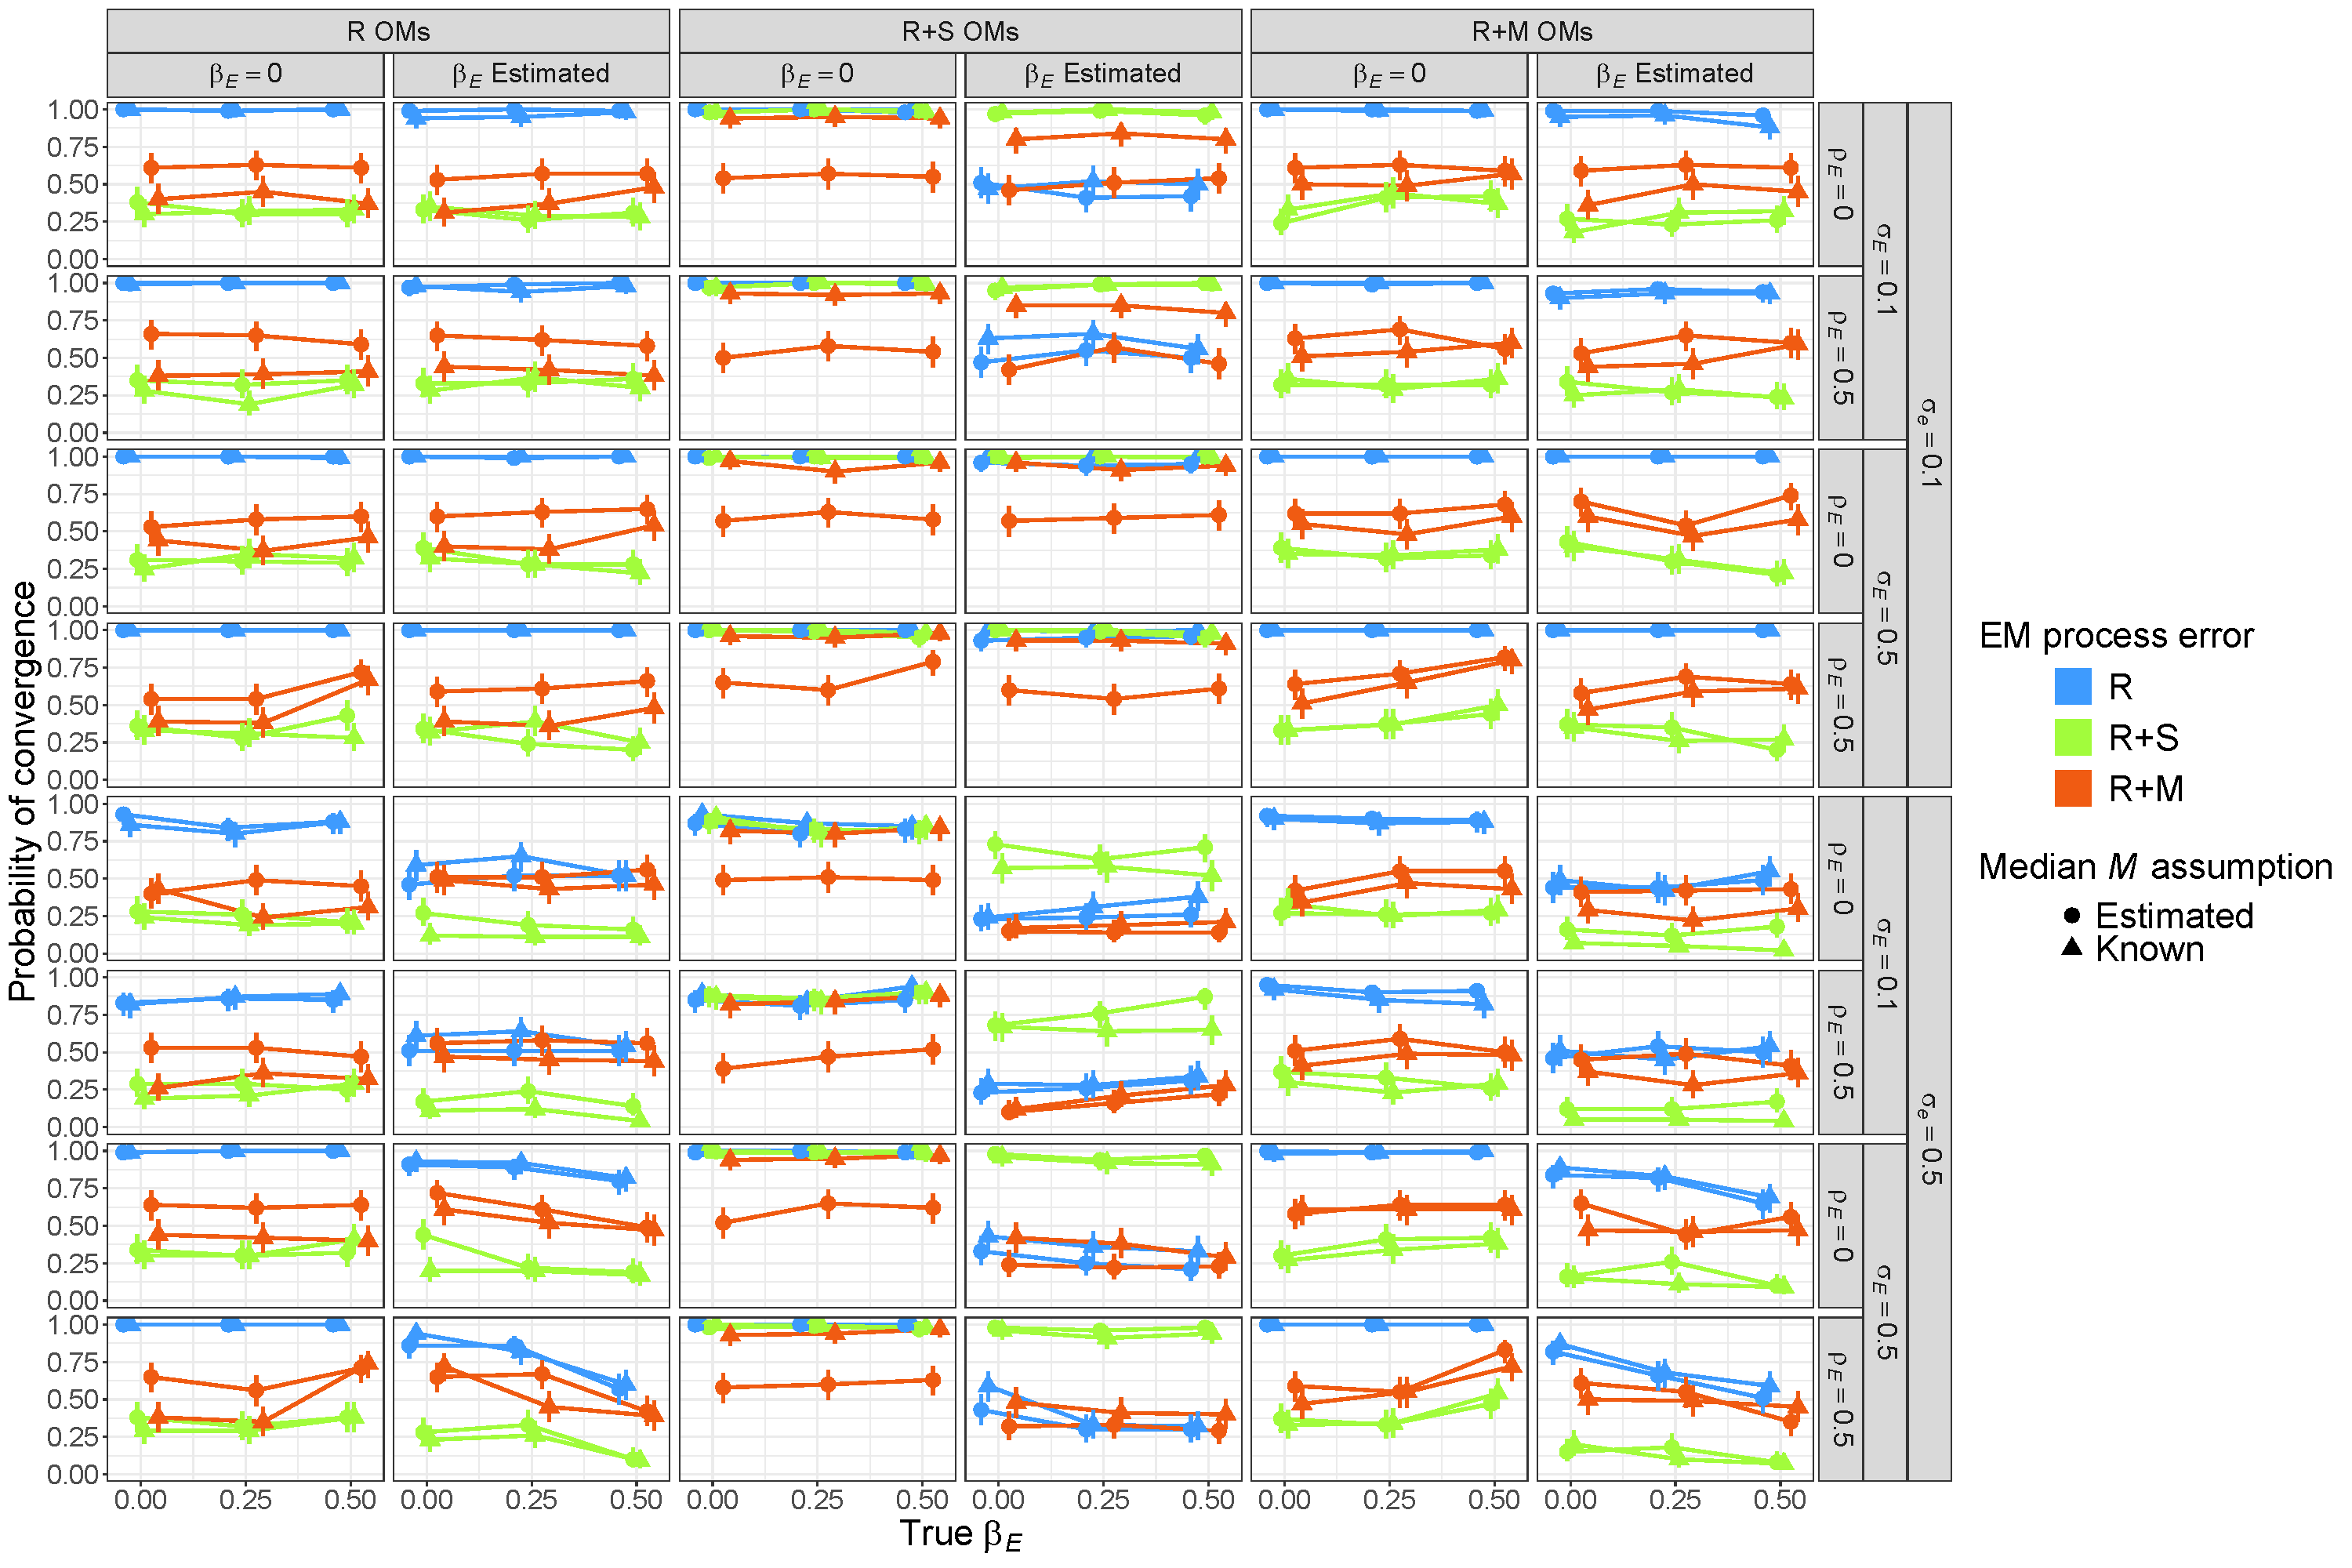
\includegraphics{convergence_main}
\end{center}
\caption{Estimated probability of fits providing Hessian-based standard errors for EMs with alternative process error assumptions, treatment of median natural mortality ($e^\beta_M$ known or estimated), and treatment of covariate effect ($\beta_E = 0$ or estimated). The OMs have R (left) and R+S (middle), or R+M (right) process error structures, alternative configurations of covariate time series structure and levels of observation uncertainty (rows), and three levels of true covariate effect on median natural mortality (x axis). All OMs had low observation error for fish population observations and temporal contrast in fishing pressure. Vertical lines represent 95\% confidence intervals.}\label{convergence}
\end{figure}
\end{landscape}

\begin{landscape}
\begin{figure}
\begin{center}
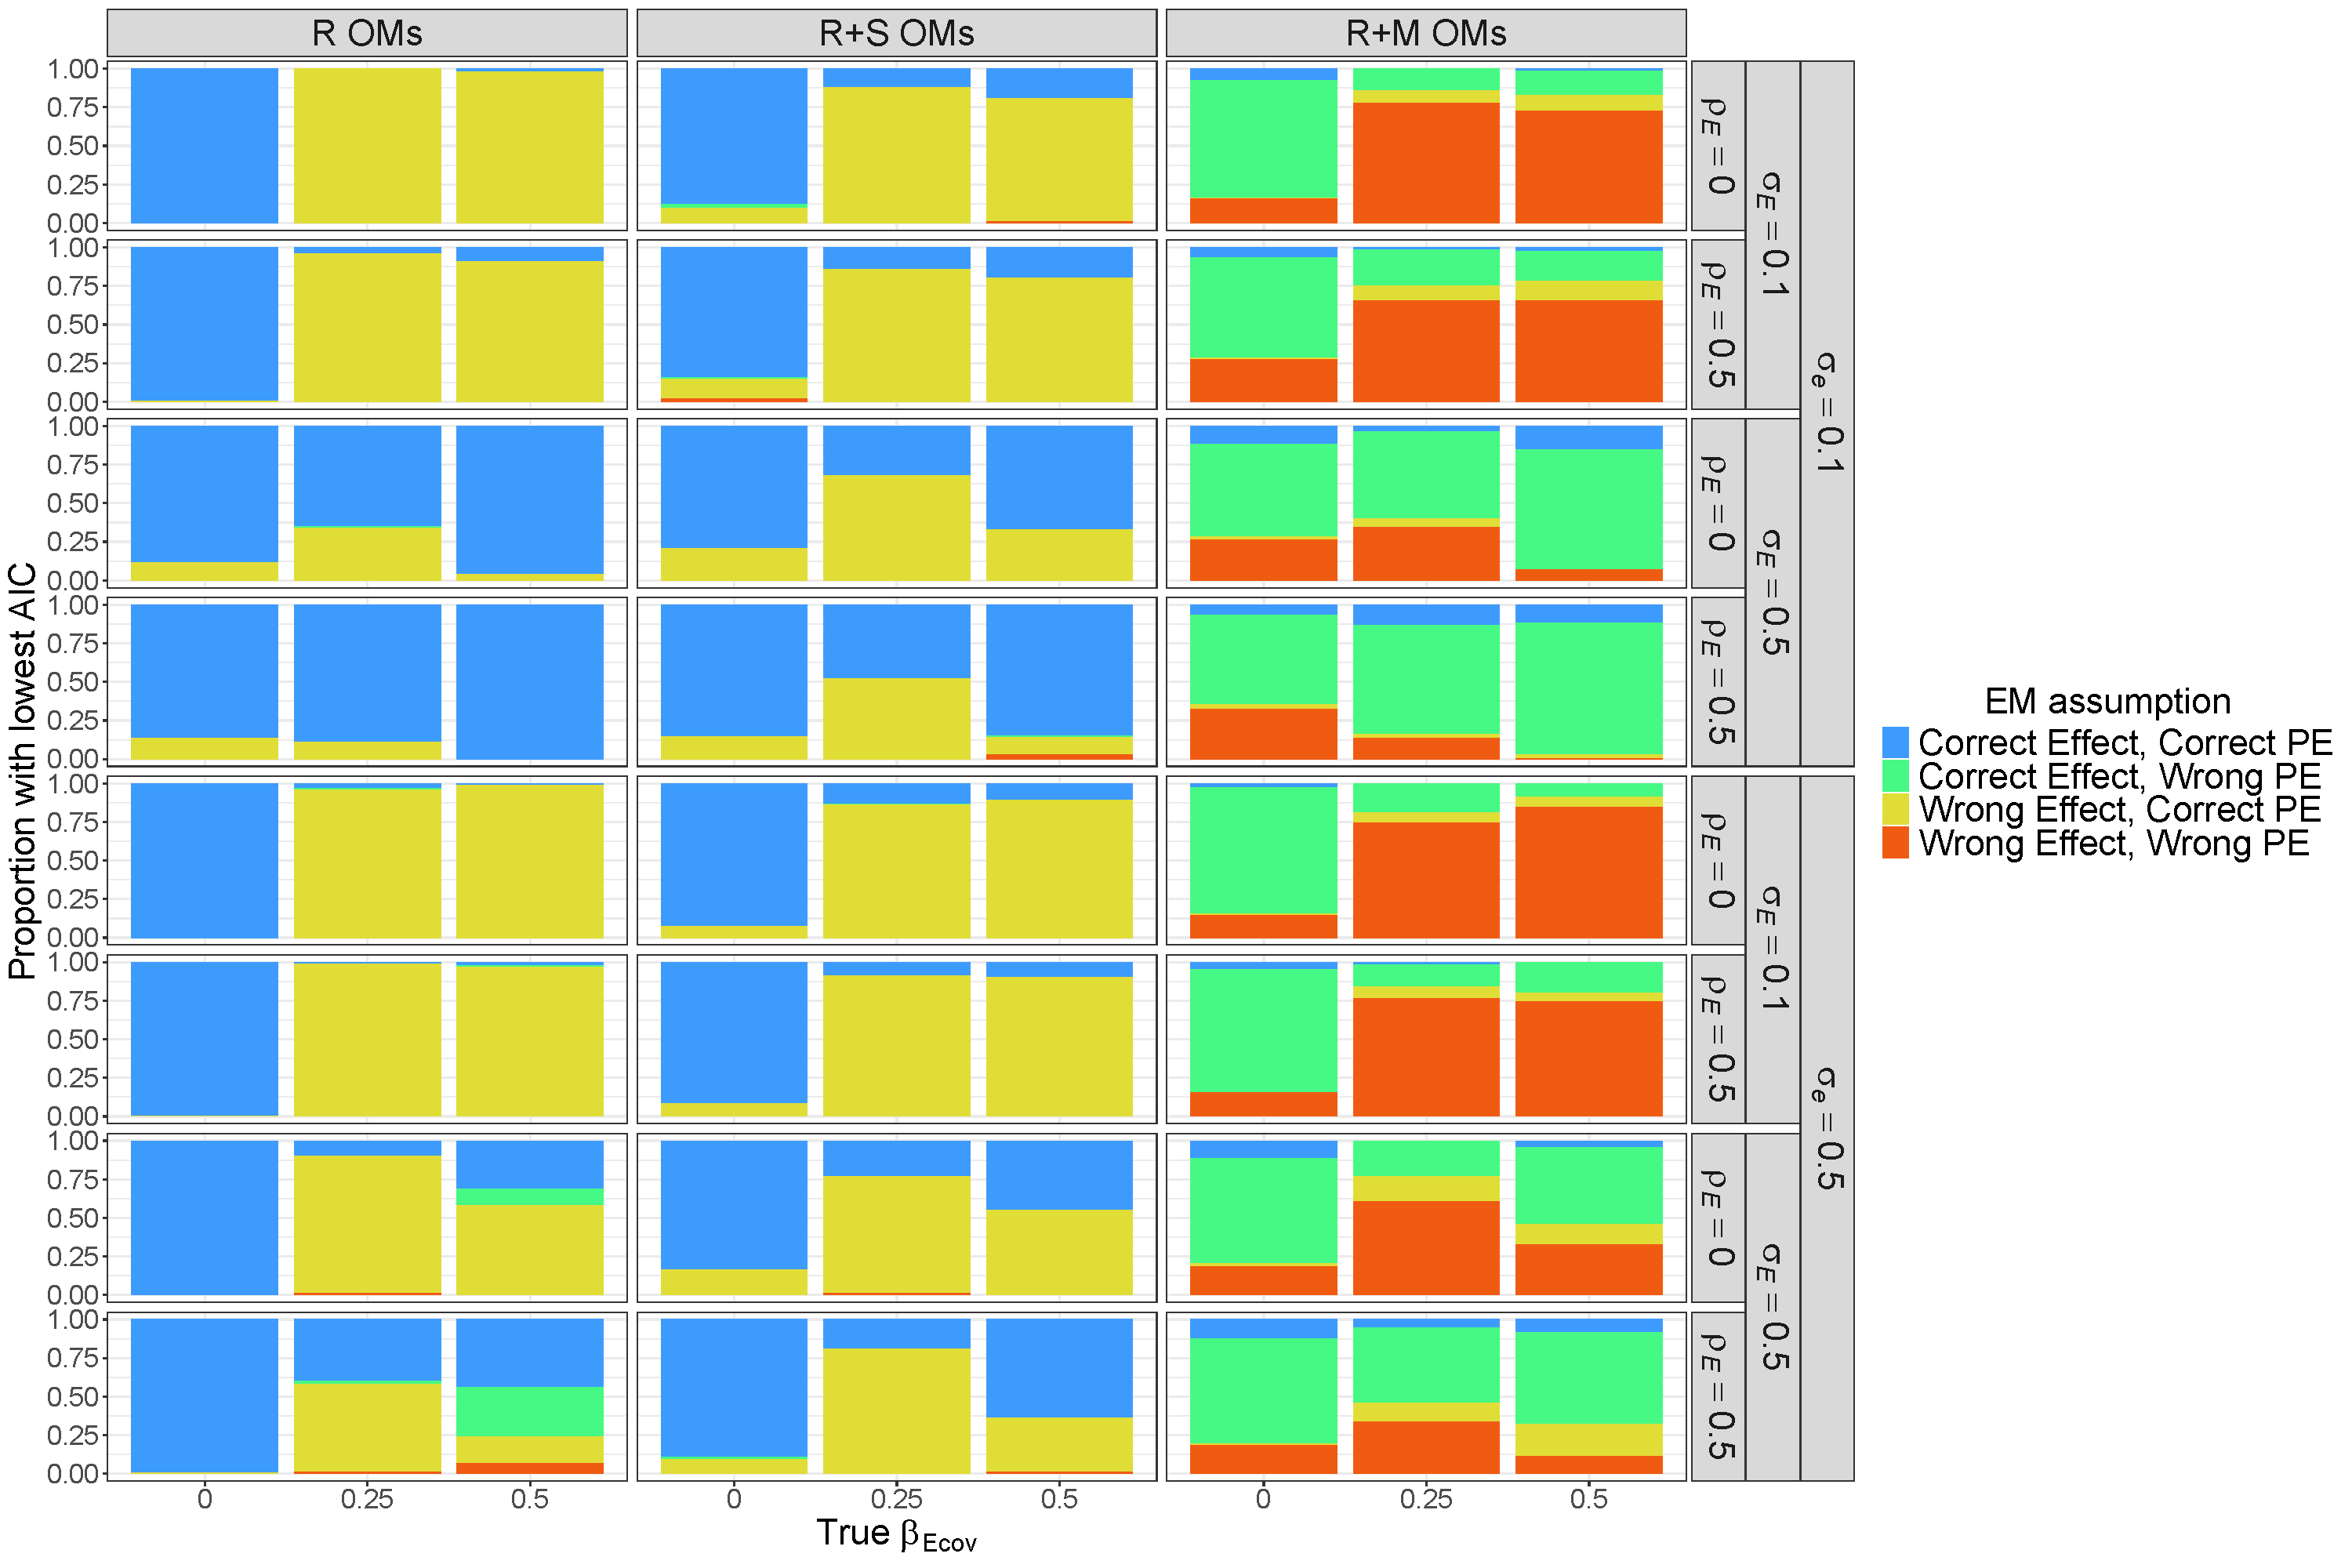
\includegraphics[height = \textheight]{aic_main}
\end{center}
\caption{For each OM, the proportion of simulated data sets where the EM type (treatment of environmental covariate effect and  assumed process error type) had the lowest AIC. All OMs had low observation error for fish population observations and temporal contrast in fishing pressure. All EMs estimated median natural mortality rate.}\label{aic}
\end{figure}
\end{landscape}

\begin{landscape}
\begin{figure}
\begin{center}
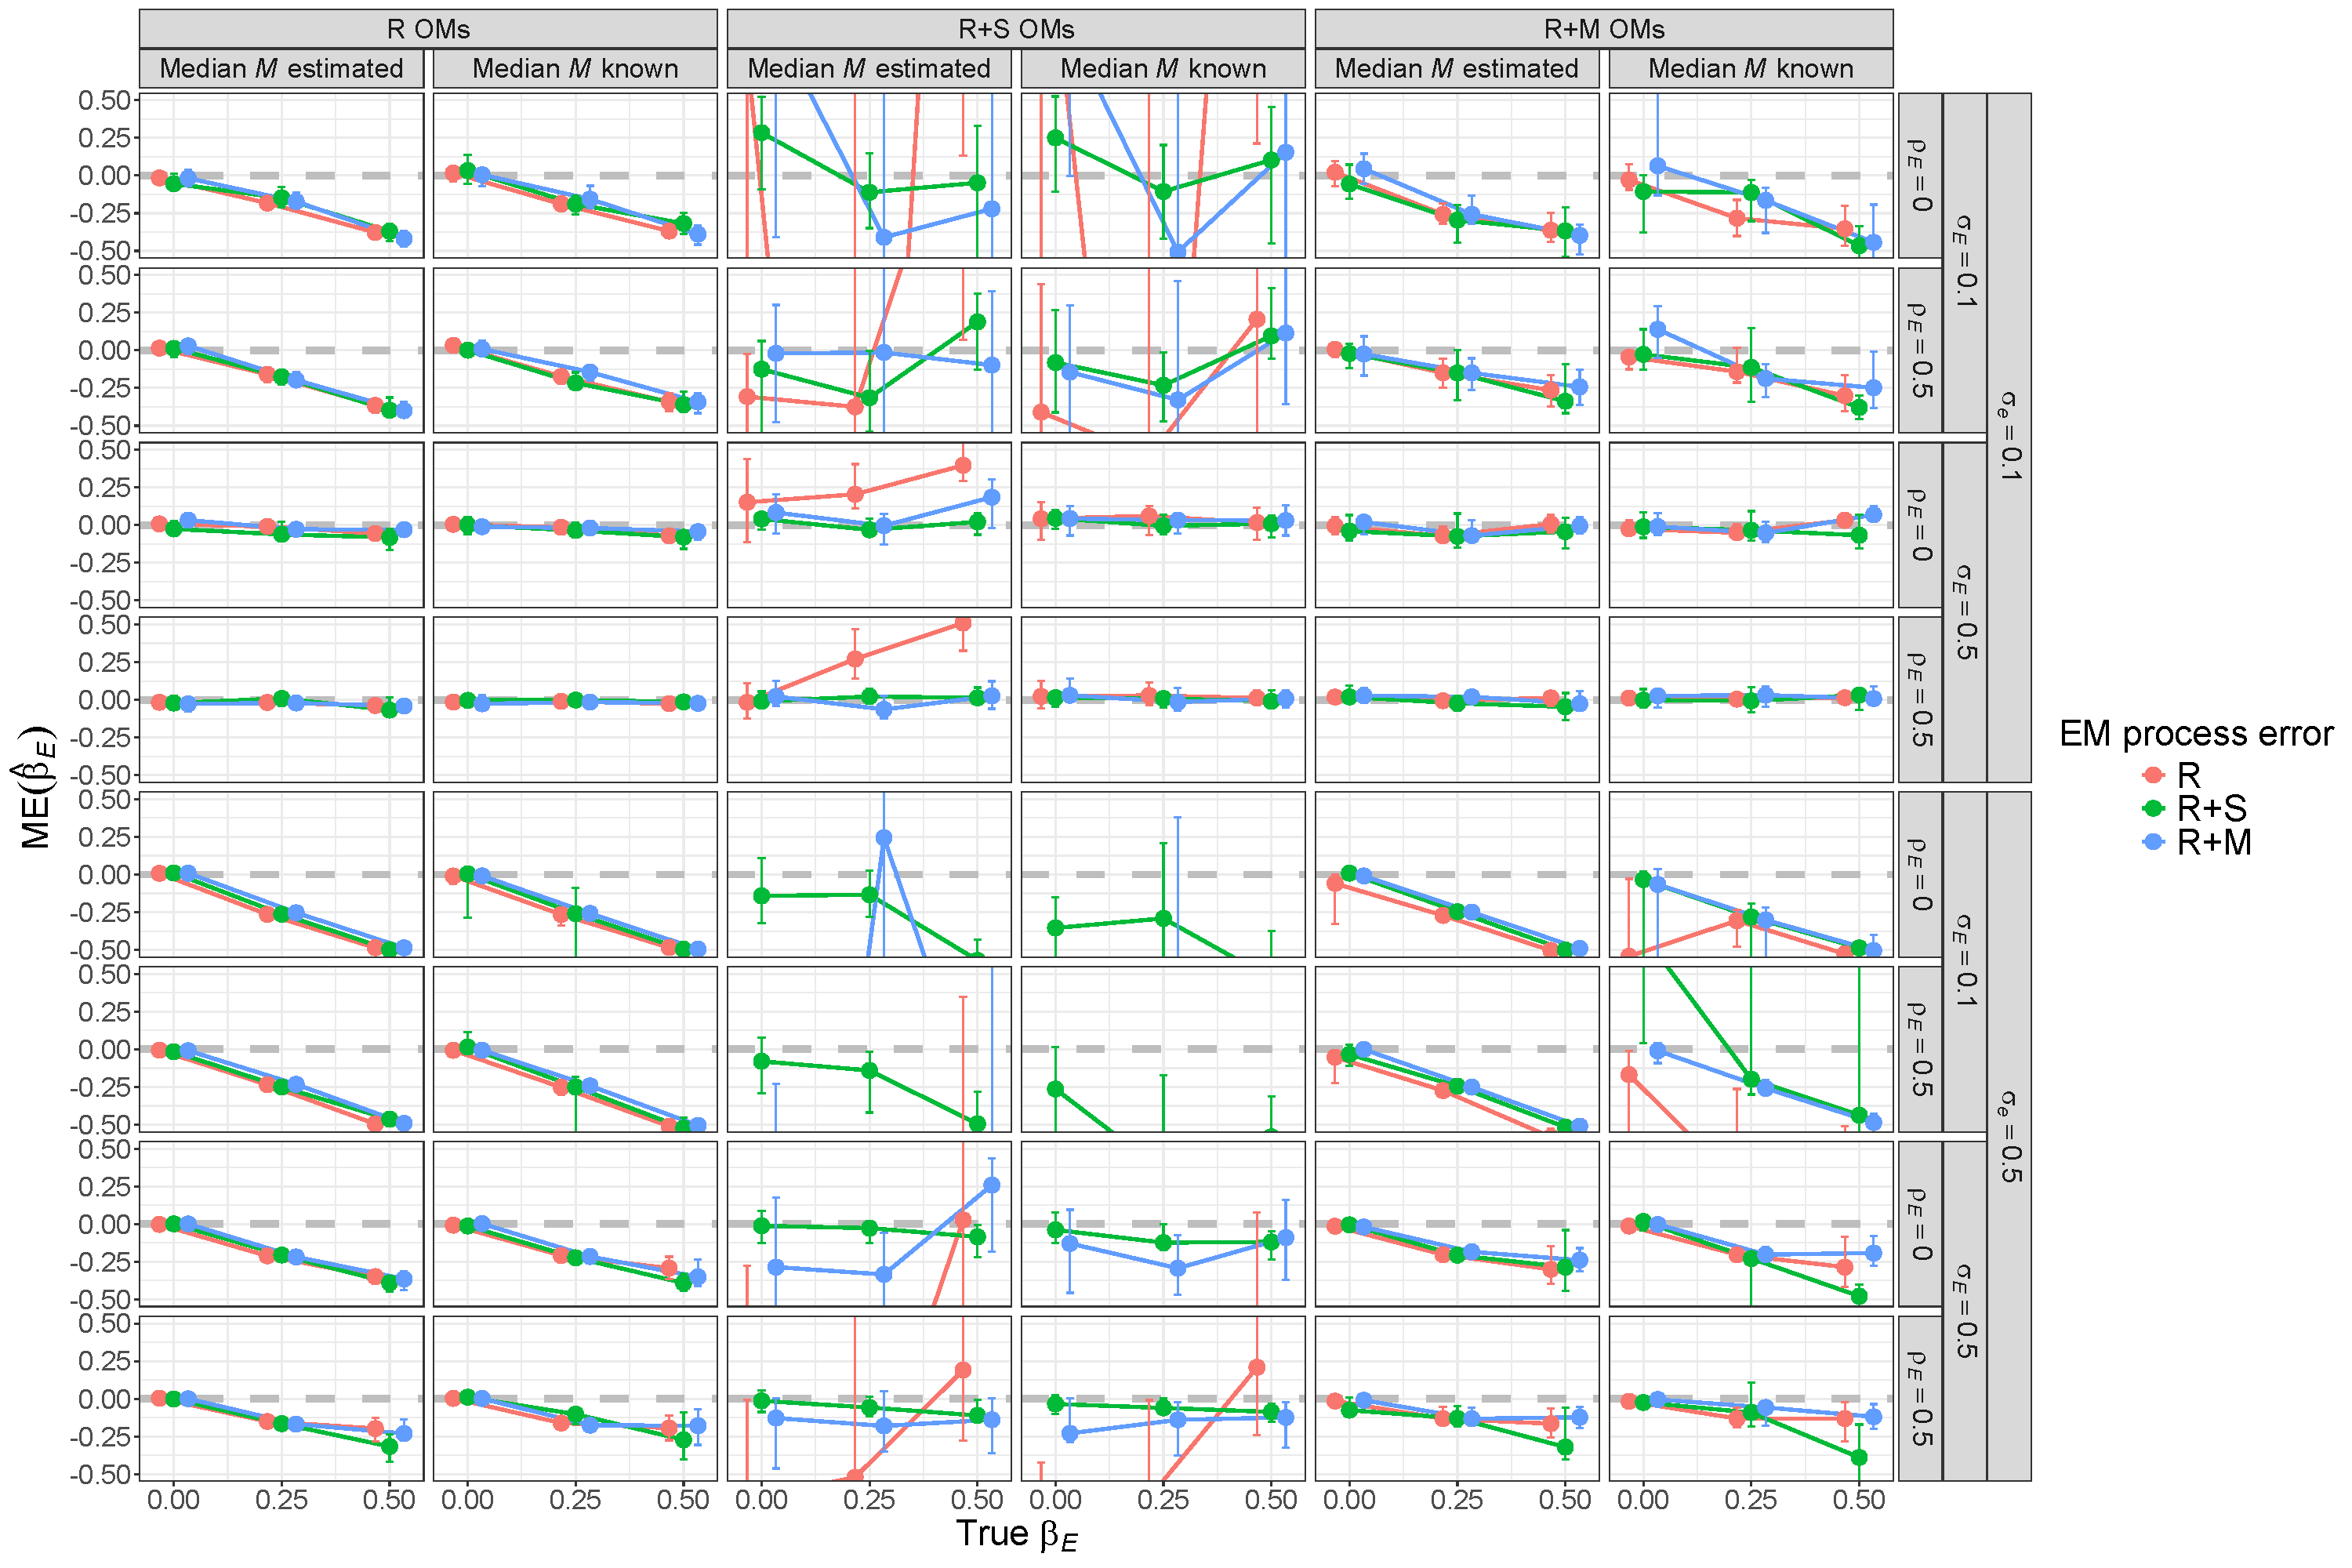
\includegraphics[height = \textheight]{beta_E_bias_main}
\end{center}
\caption{Median error (ME) of estimates of environmental effect on natural mortality $\beta_E$ from fitting EMs with alternative process error assumptions and treatment of median natural mortality ($e^\beta_M$ known or estimated). All OMs had low observation error and contrast in fishing mortality. Vertical lines represent 95\% confidence intervals.}\label{beta_E_bias}
\end{figure}
\end{landscape}

\begin{landscape}
\begin{figure}
\begin{center}
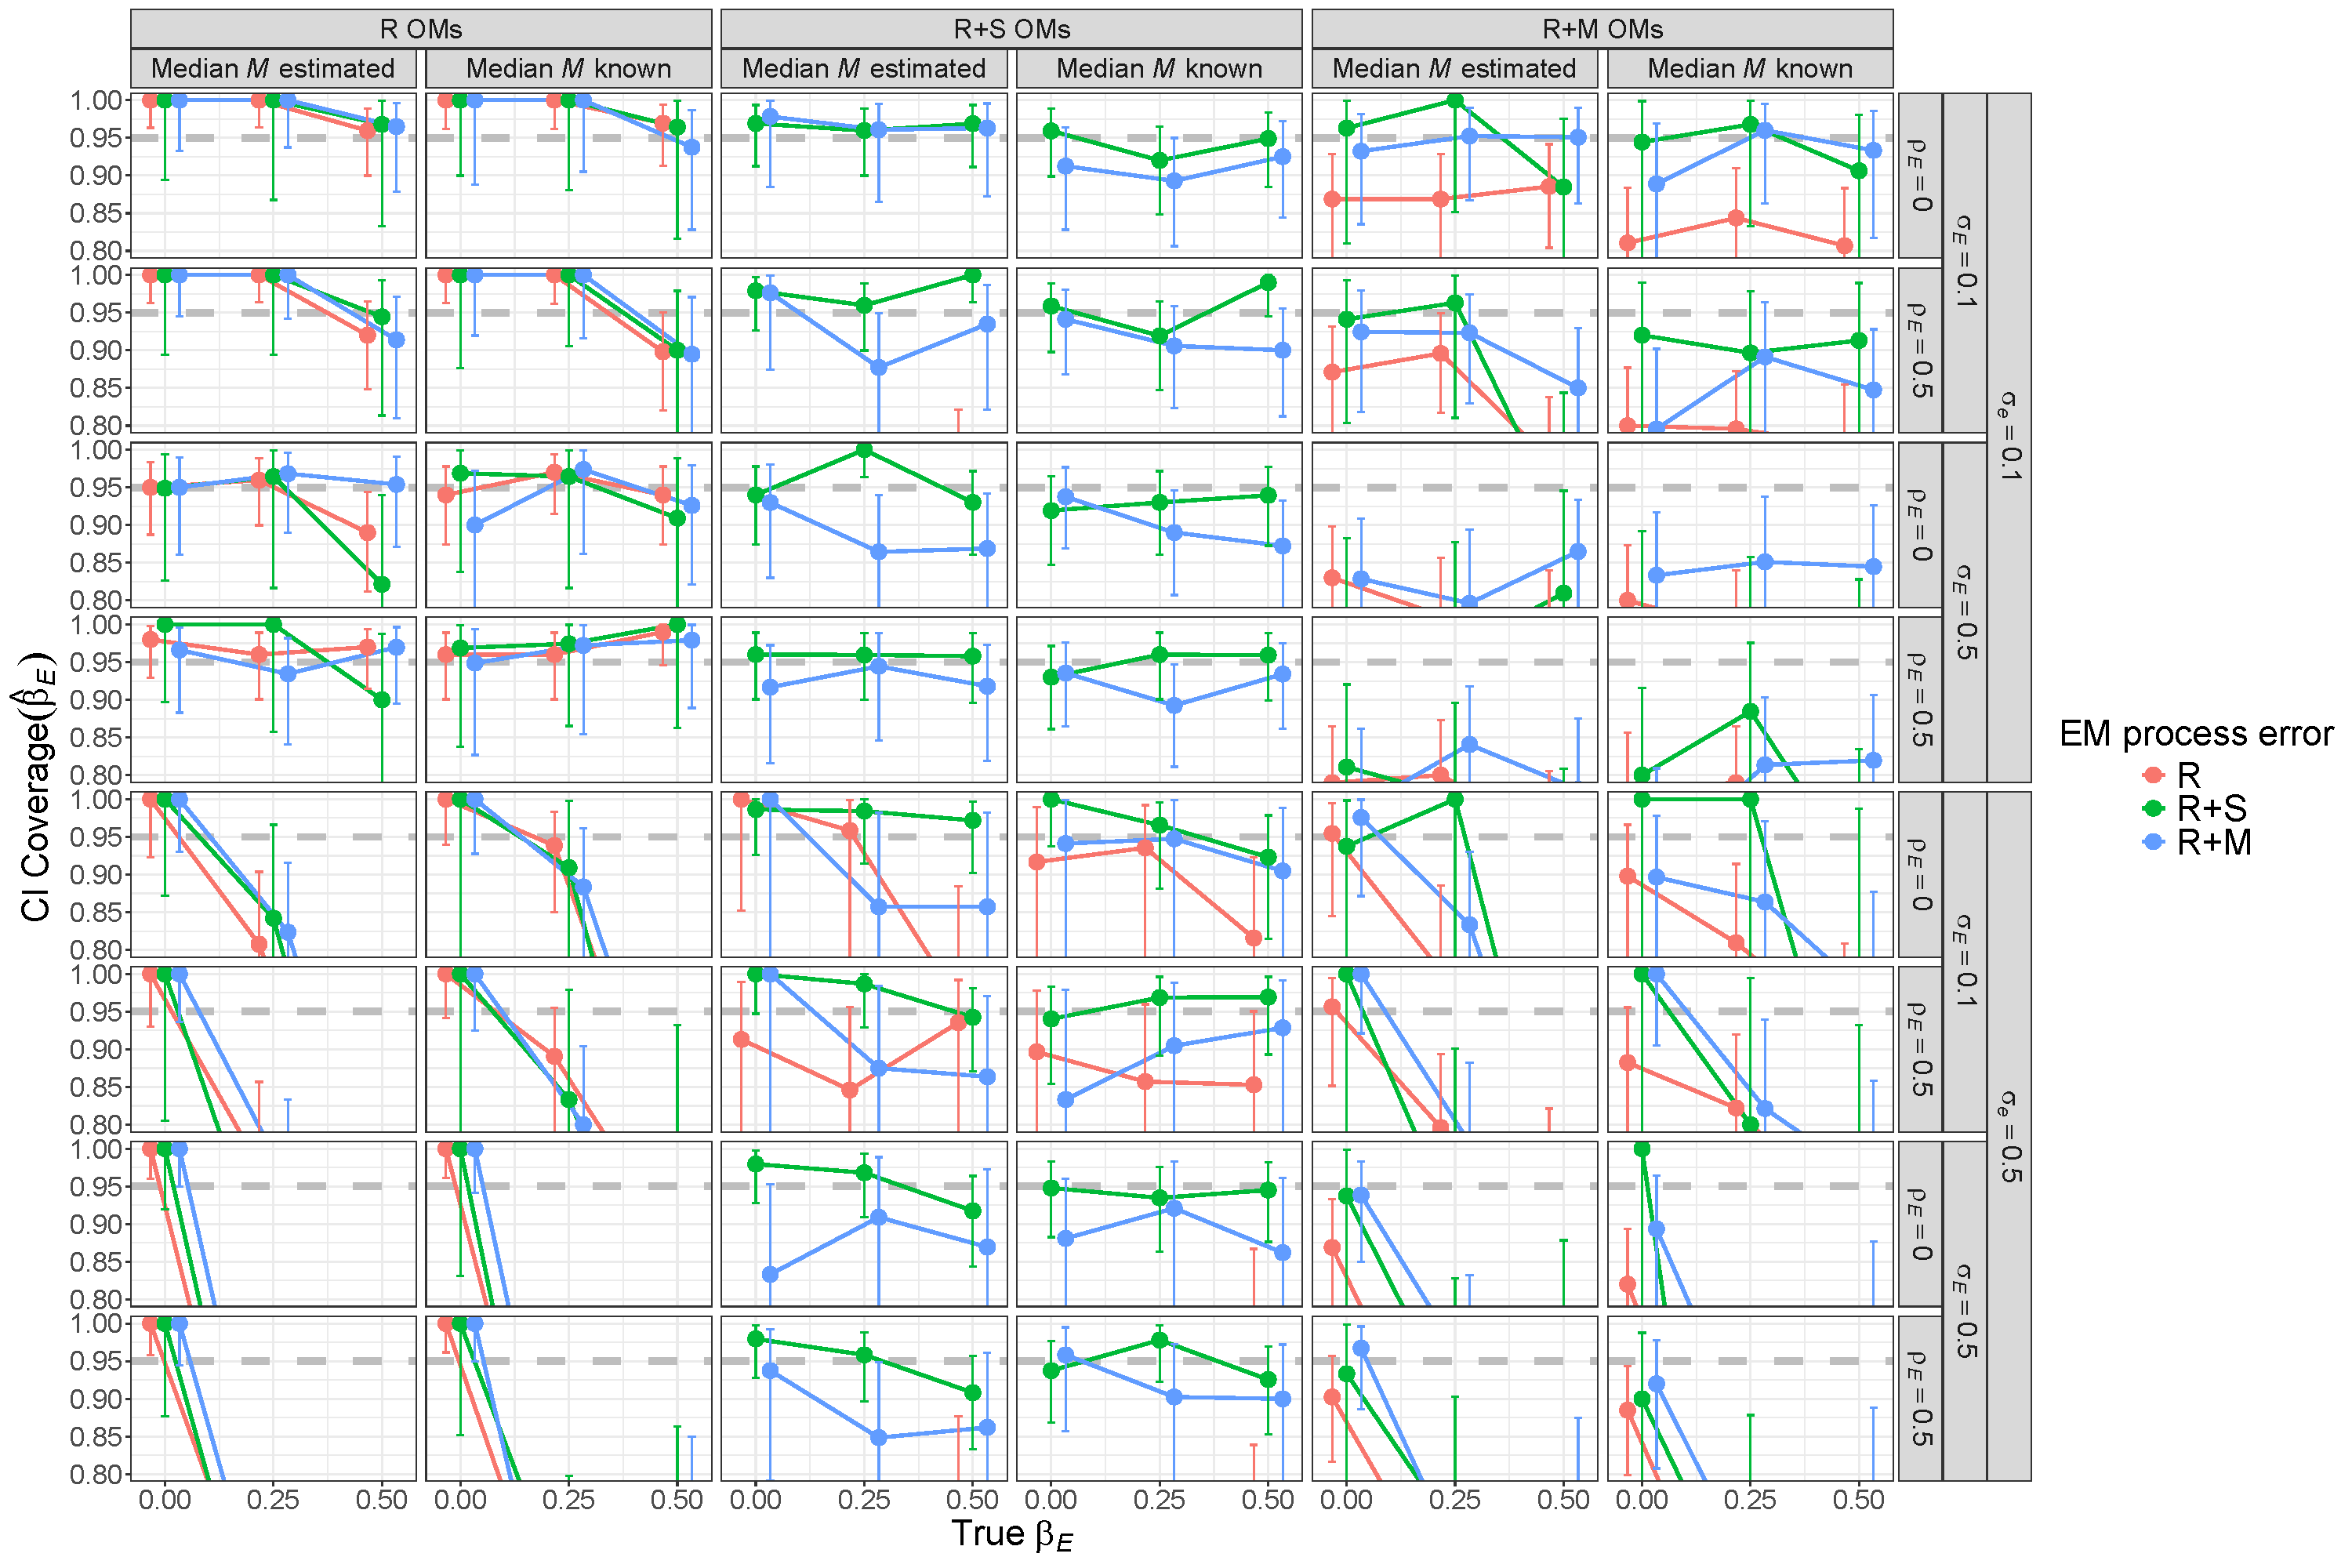
\includegraphics[height = \textheight]{beta_E_CI_coverage_main}
\end{center}
\caption{Probability of 95\% confidence interval for $\beta_E$ containing the true value for EMs with alternative process error assumptions and treatment of median natural mortality ($e^\beta_M$ known or estimated). All OMs had low observation error and contrast in fishing mortality. Vertical lines represent 95\% confidence intervals.}\label{beta_E_CI_coverage}
\end{figure}
\end{landscape}

\begin{landscape}
\begin{figure}
\begin{center}
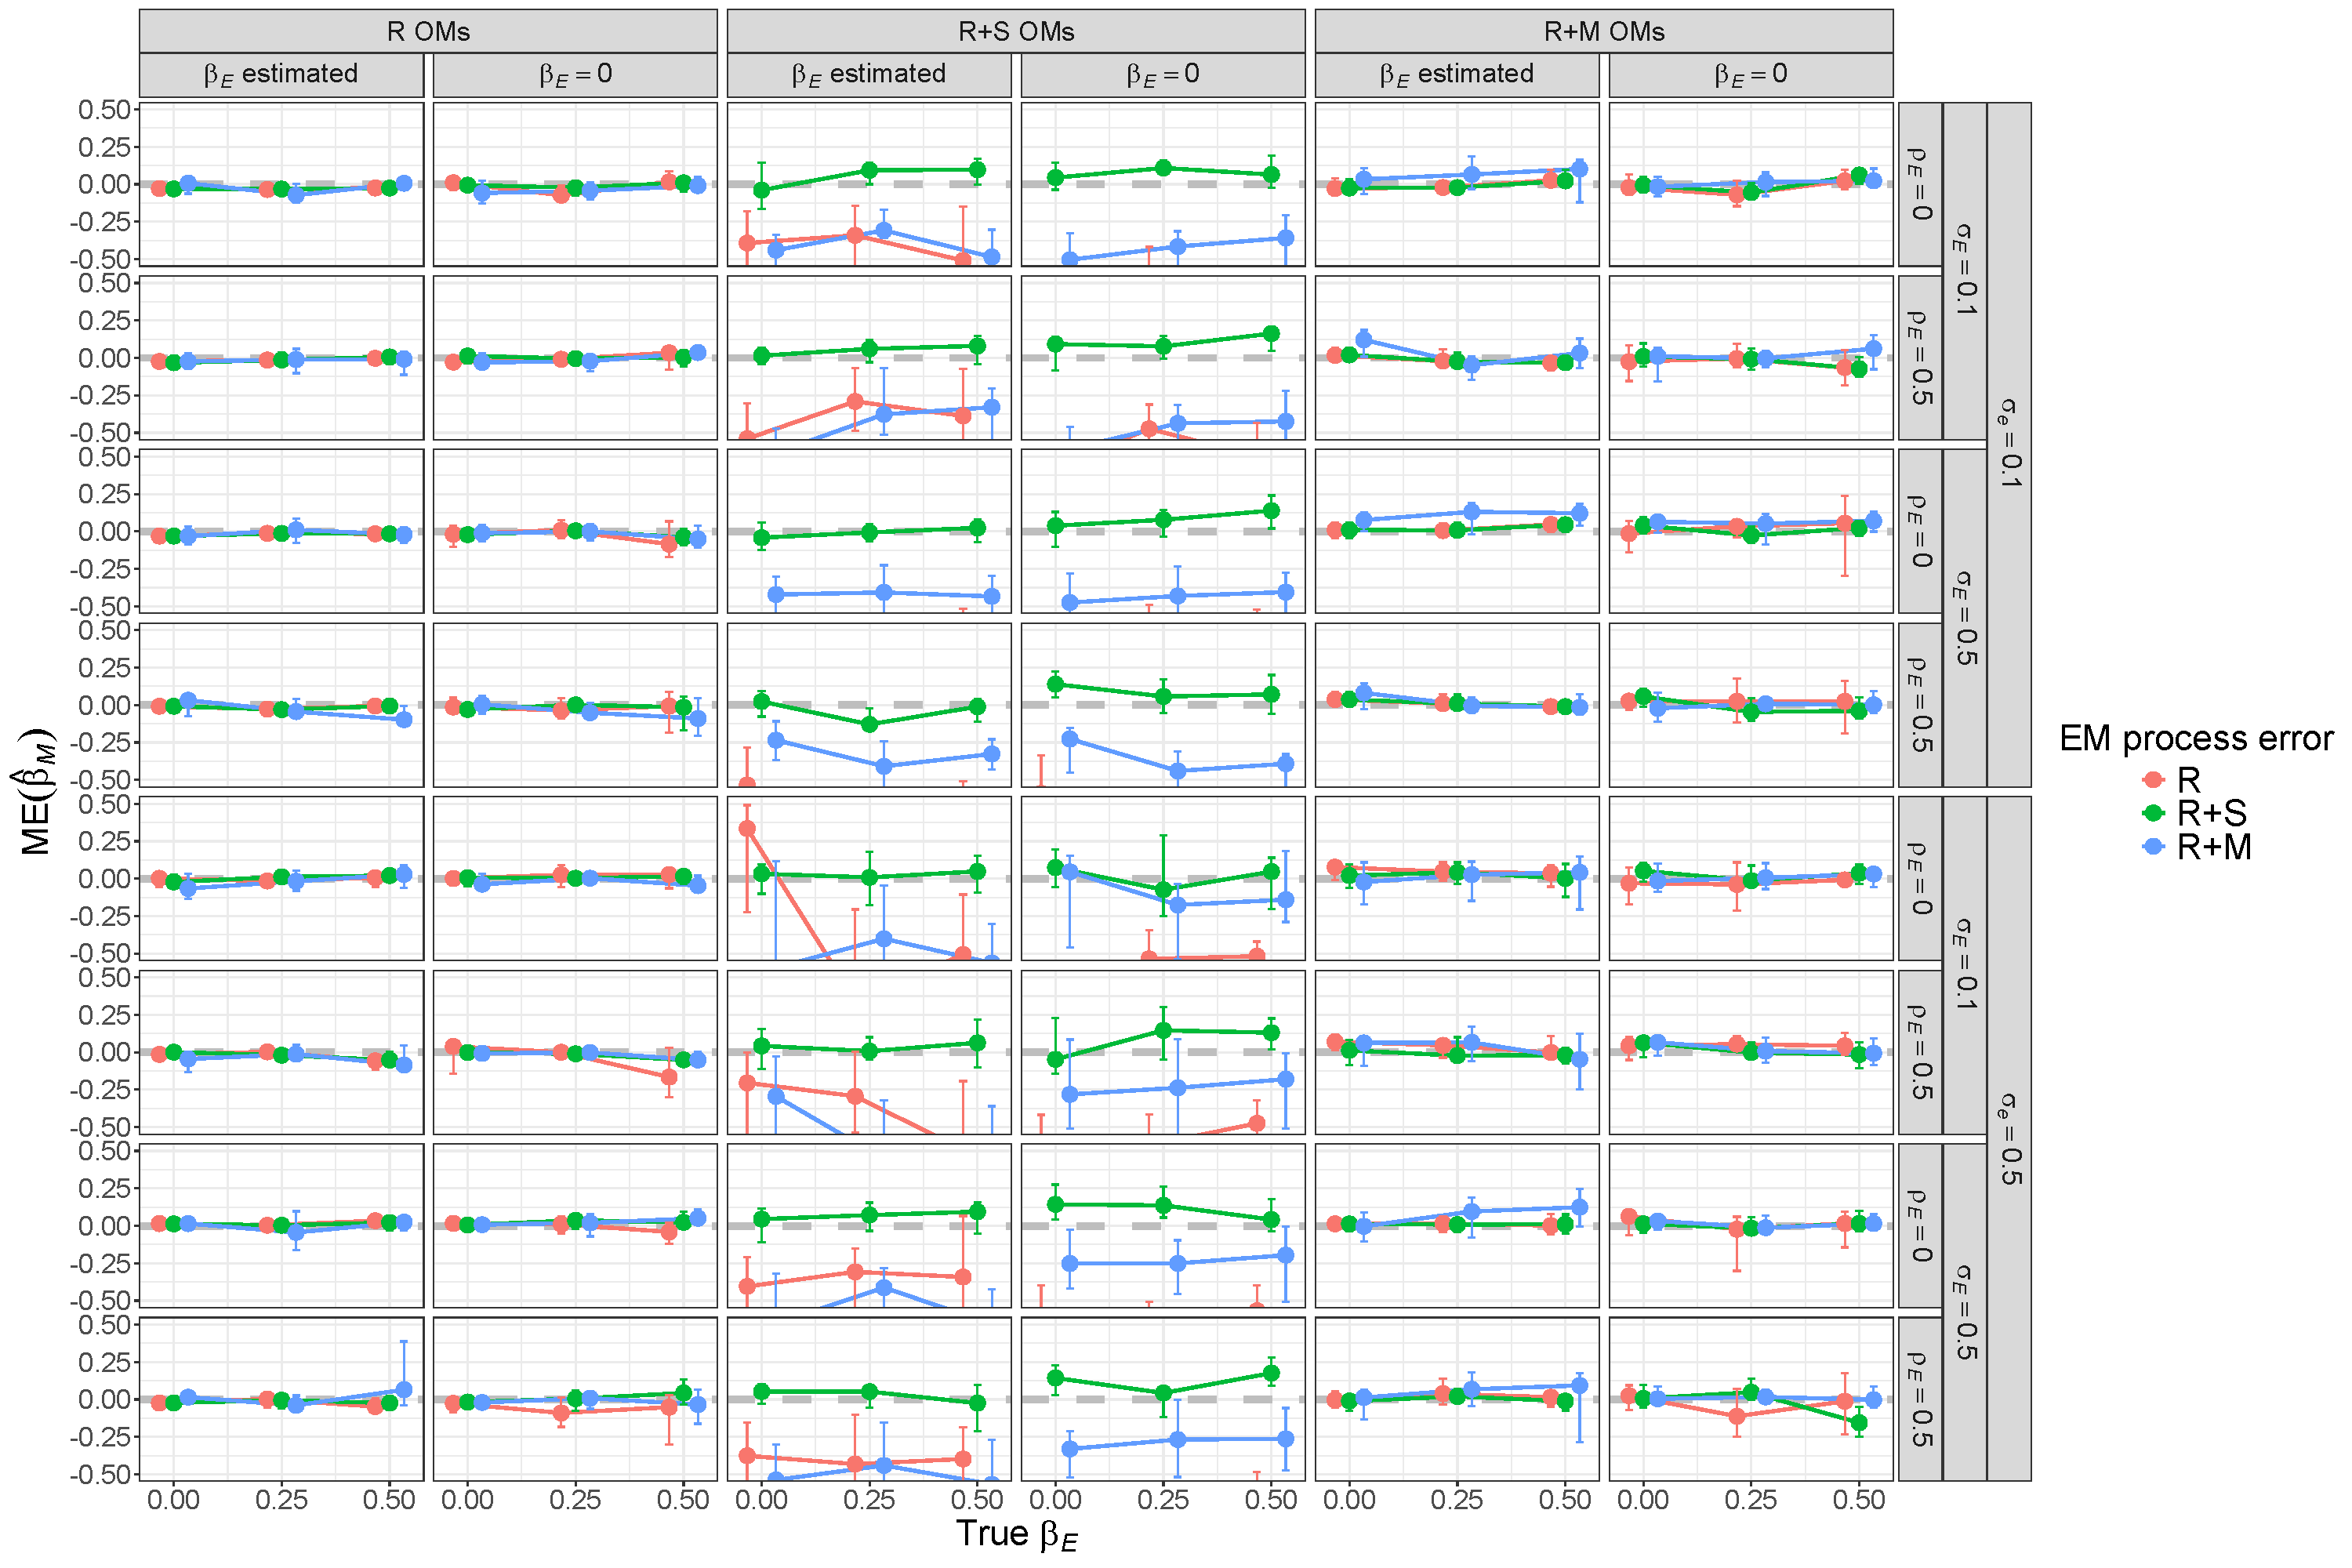
\includegraphics[height = \textheight]{beta_M_bias_main}
\end{center}
\caption{Median error (ME) of estimates of $\beta_M$ from fitting EMs with alternative process error assumptions and treatment of covariate effect ($\beta_E = 0$ or estimated). All OMs had low observation error and contrast in fishing mortality. Vertical lines represent 95\% confidence intervals.}\label{beta_M_bias}
\end{figure}
\end{landscape}

\begin{landscape}
\begin{figure}
\begin{center}
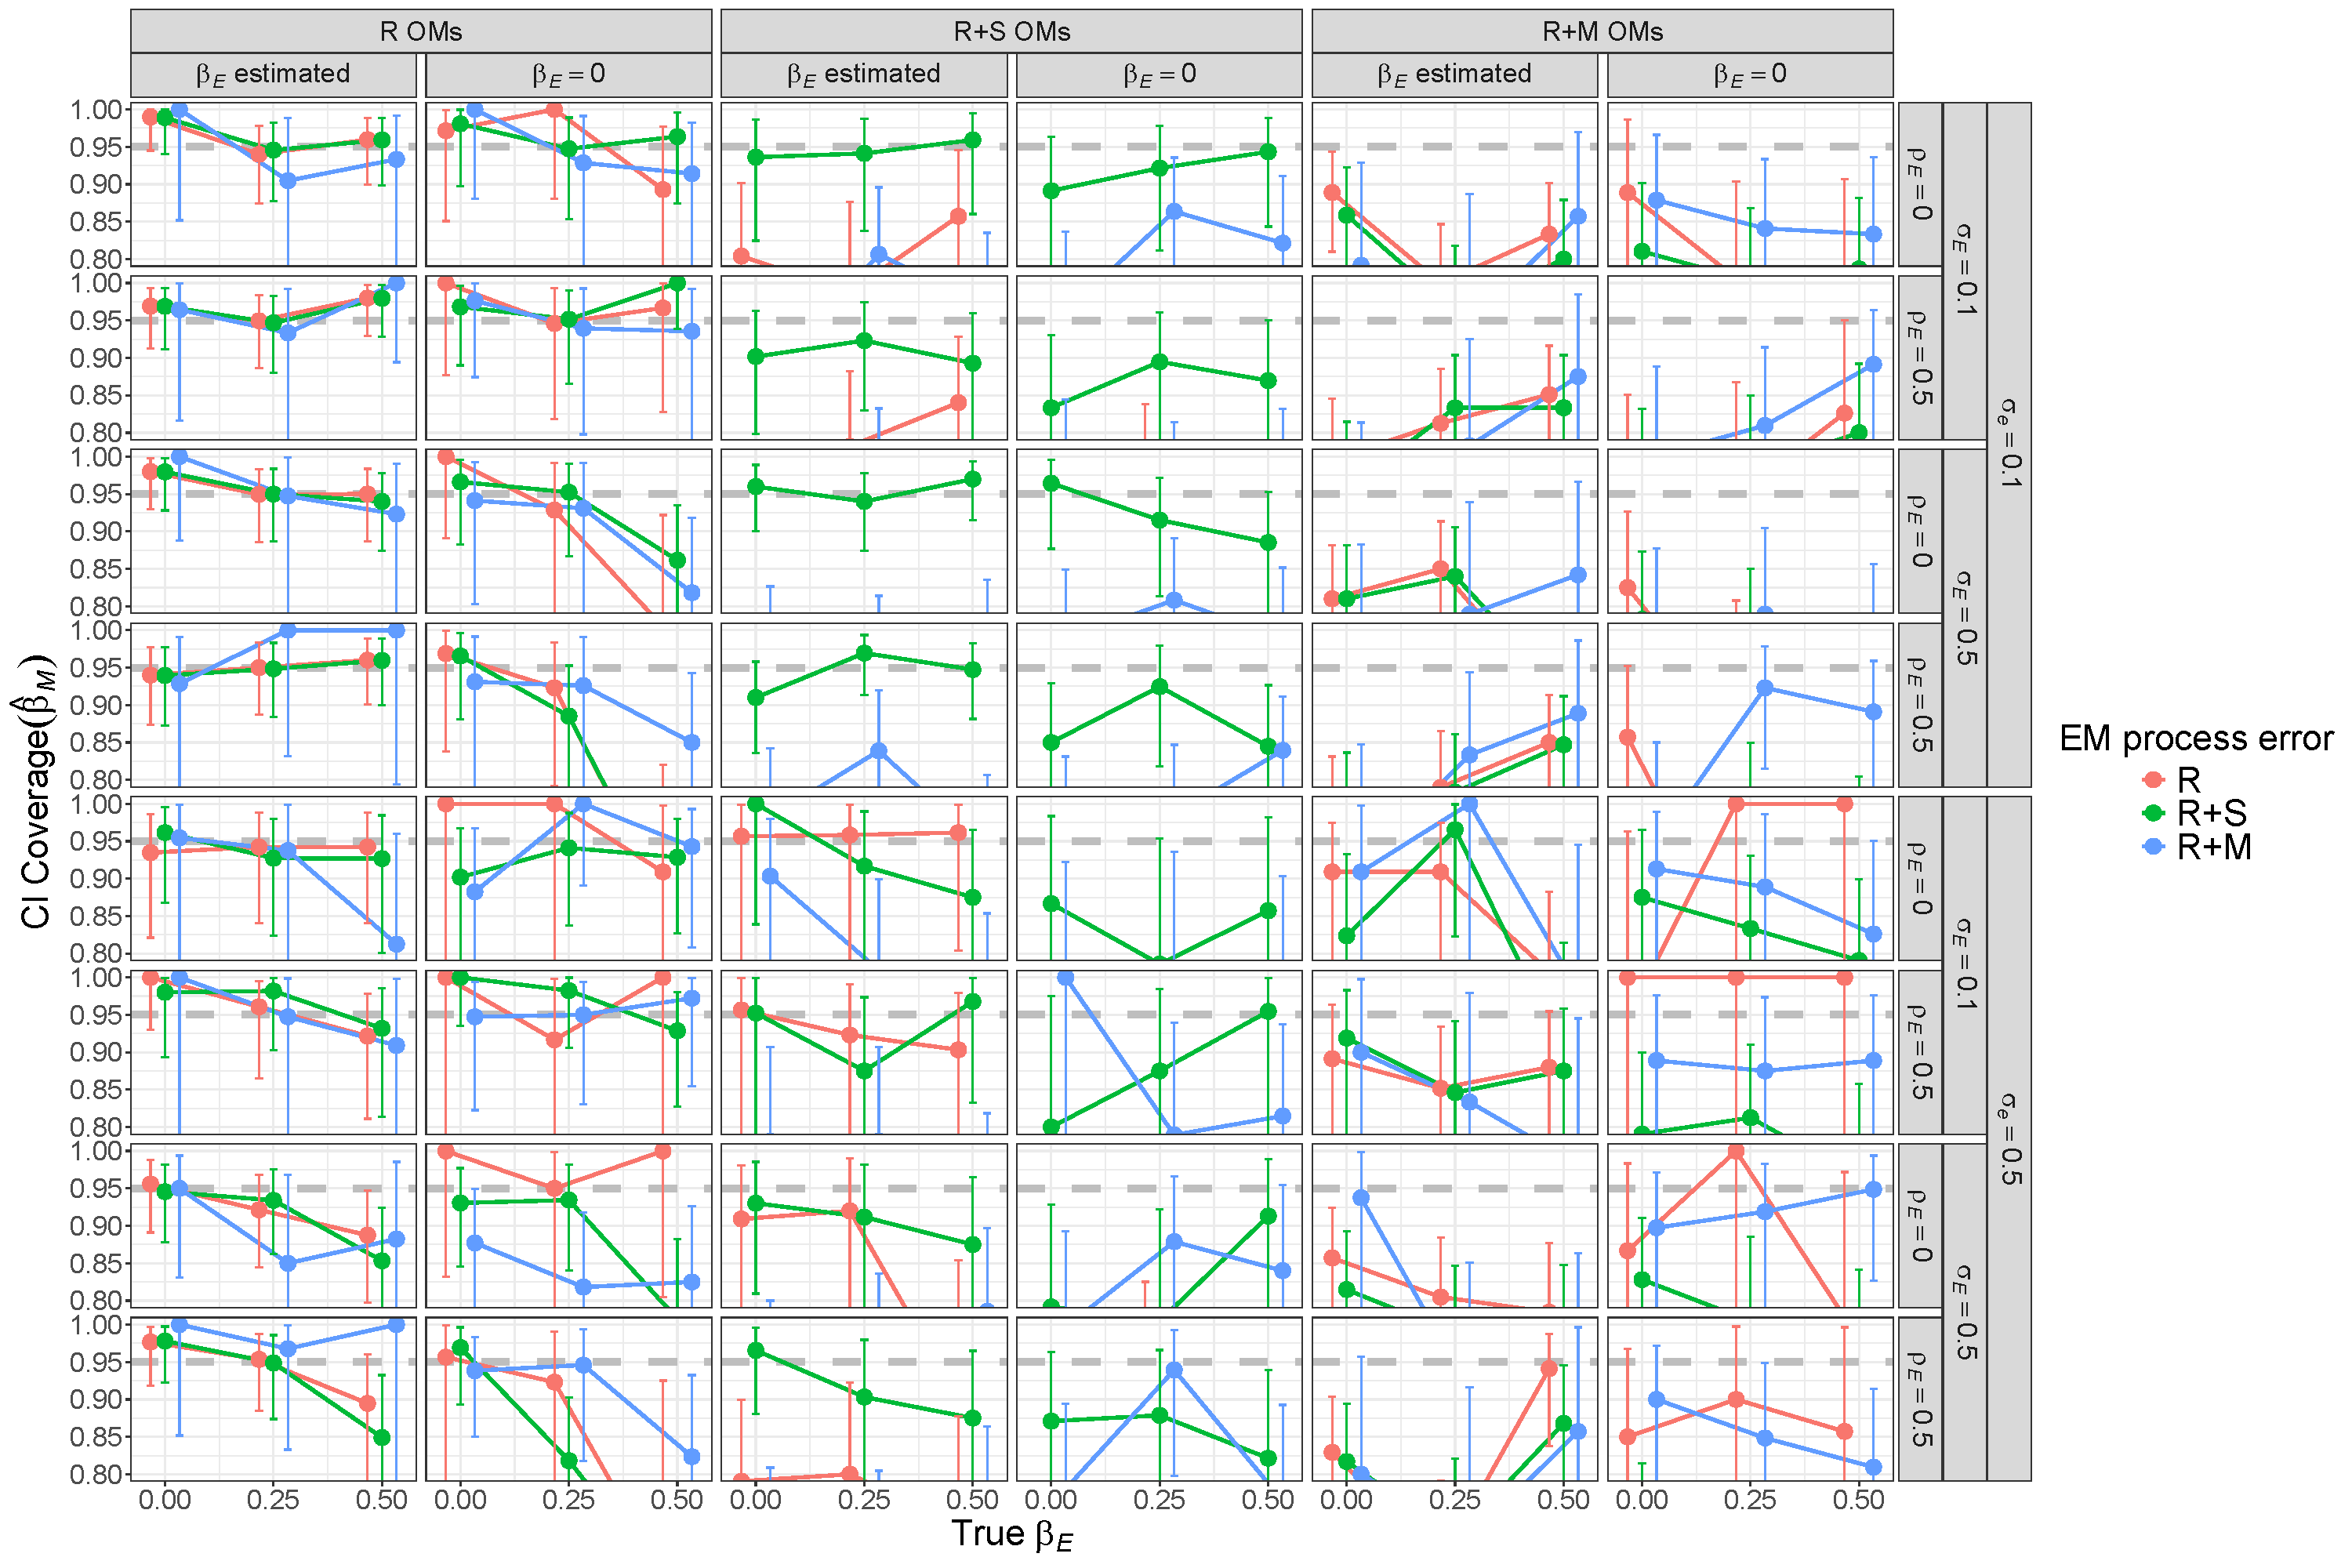
\includegraphics[height = \textheight]{beta_M_CI_coverage_main}
\end{center}
\caption{Probability of 95\% confidence interval for $\beta_M$ containing the true value for EMs with alternative process error assumptions and treatment of covariate effect ($\beta_E = 0$ or estimated). All OMs had low observation error and contrast in fishing mortality. Vertical lines represent 95\% confidence intervals.}\label{beta_M_CI_coverage}
\end{figure}
\end{landscape}

\begin{landscape}
\begin{figure}
\begin{center}
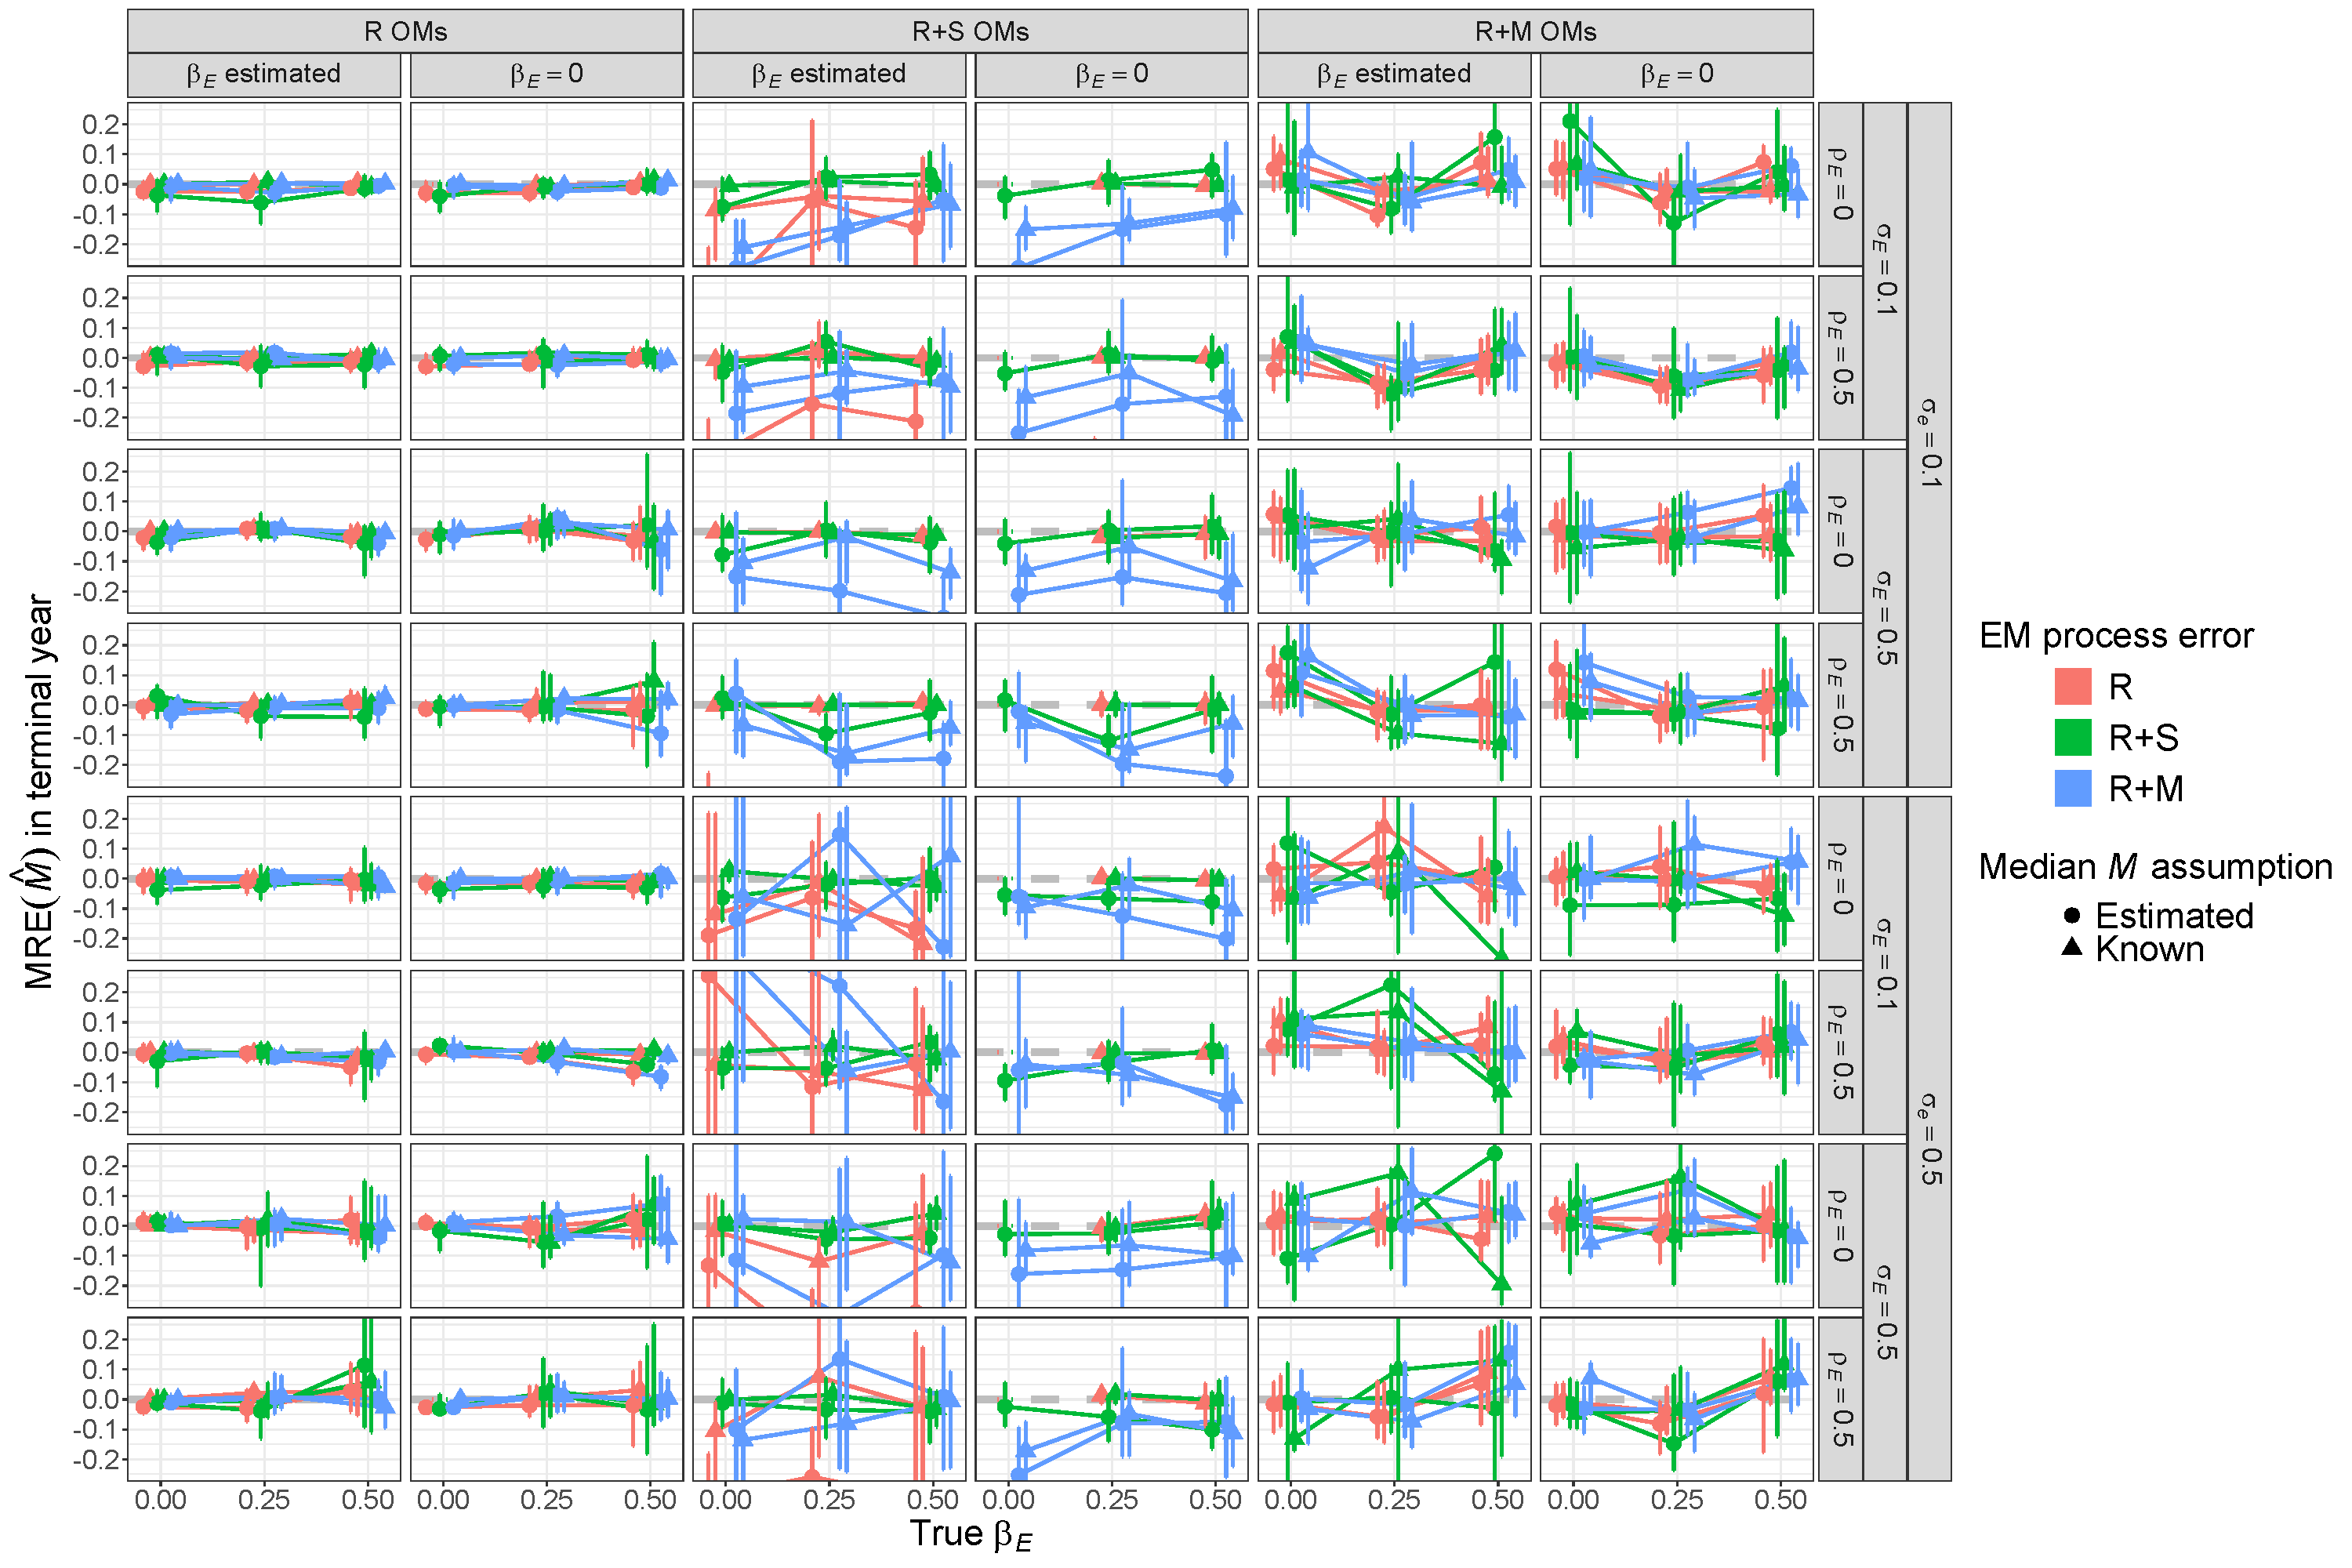
\includegraphics[height = \textheight]{terminal_year_M_bias_main}
\end{center}
\caption{Median relative error (MRE) of estimates of natural mortality rate in the terminal year for EMs with alternative process error assumptions, treatment of covariate effect ($\beta_E = 0$ or estimated), and treatment of median natural mortality parameter ($\beta_M$ estimated or known).  All OMs had low observation error and contrast in fishing mortality.}\label{terminal_M_bias}
\end{figure}
\end{landscape}

\begin{landscape}
\begin{figure}
\begin{center}
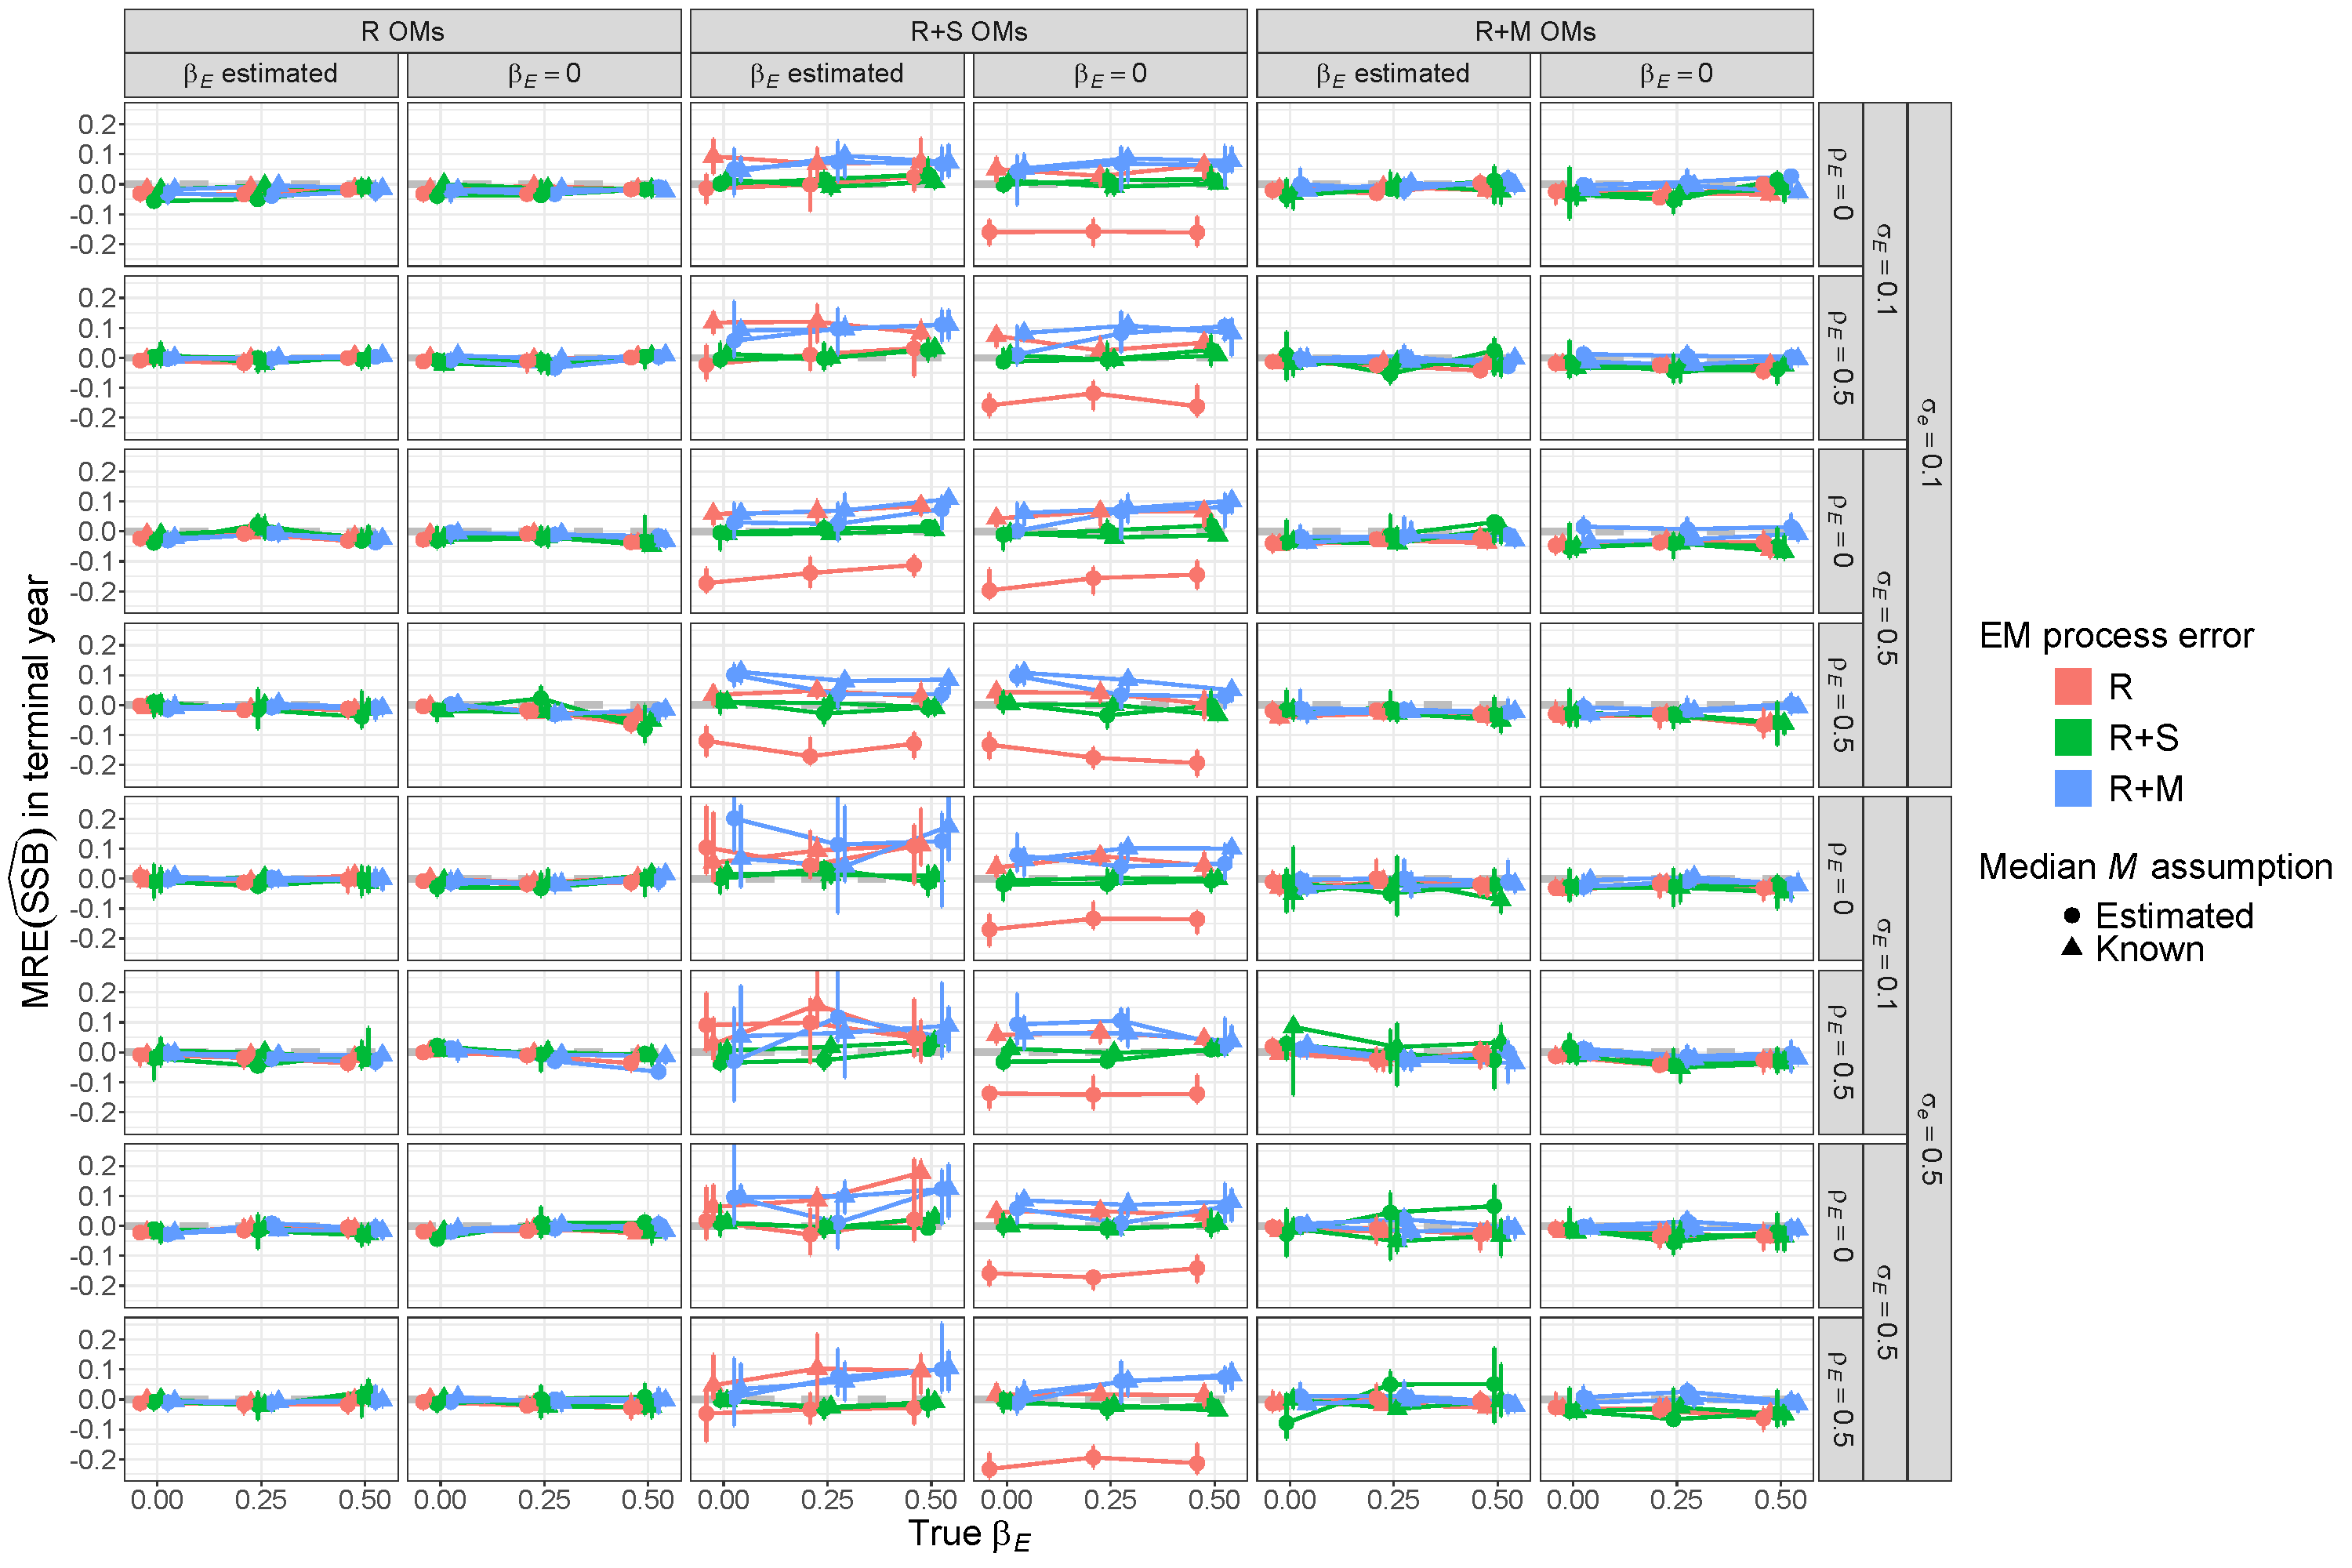
\includegraphics[height = \textheight]{terminal_year_ssb_bias_main}
\end{center}
\caption{Median relative error (MRE) of estimates of spawning stock biomass (SSB) in the terminal year for EMs with alternative process error assumptions, treatment of covariate effect ($\beta_E = 0$ or estimated), and treatment of median natural mortality parameter ($\beta_M$ estimated or known). All OMs had low observation error and contrast in fishing mortality.}\label{terminal_ssb_bias}
\end{figure}
\end{landscape}

\hypertarget{supplemental-materials}{%
\section*{Supplemental Materials}\label{supplemental-materials}}
\addcontentsline{toc}{section}{Supplemental Materials}

\setcounter{figure}{0}
\renewcommand\thefigure{S\arabic{figure}}

\begin{figure}
\begin{center}
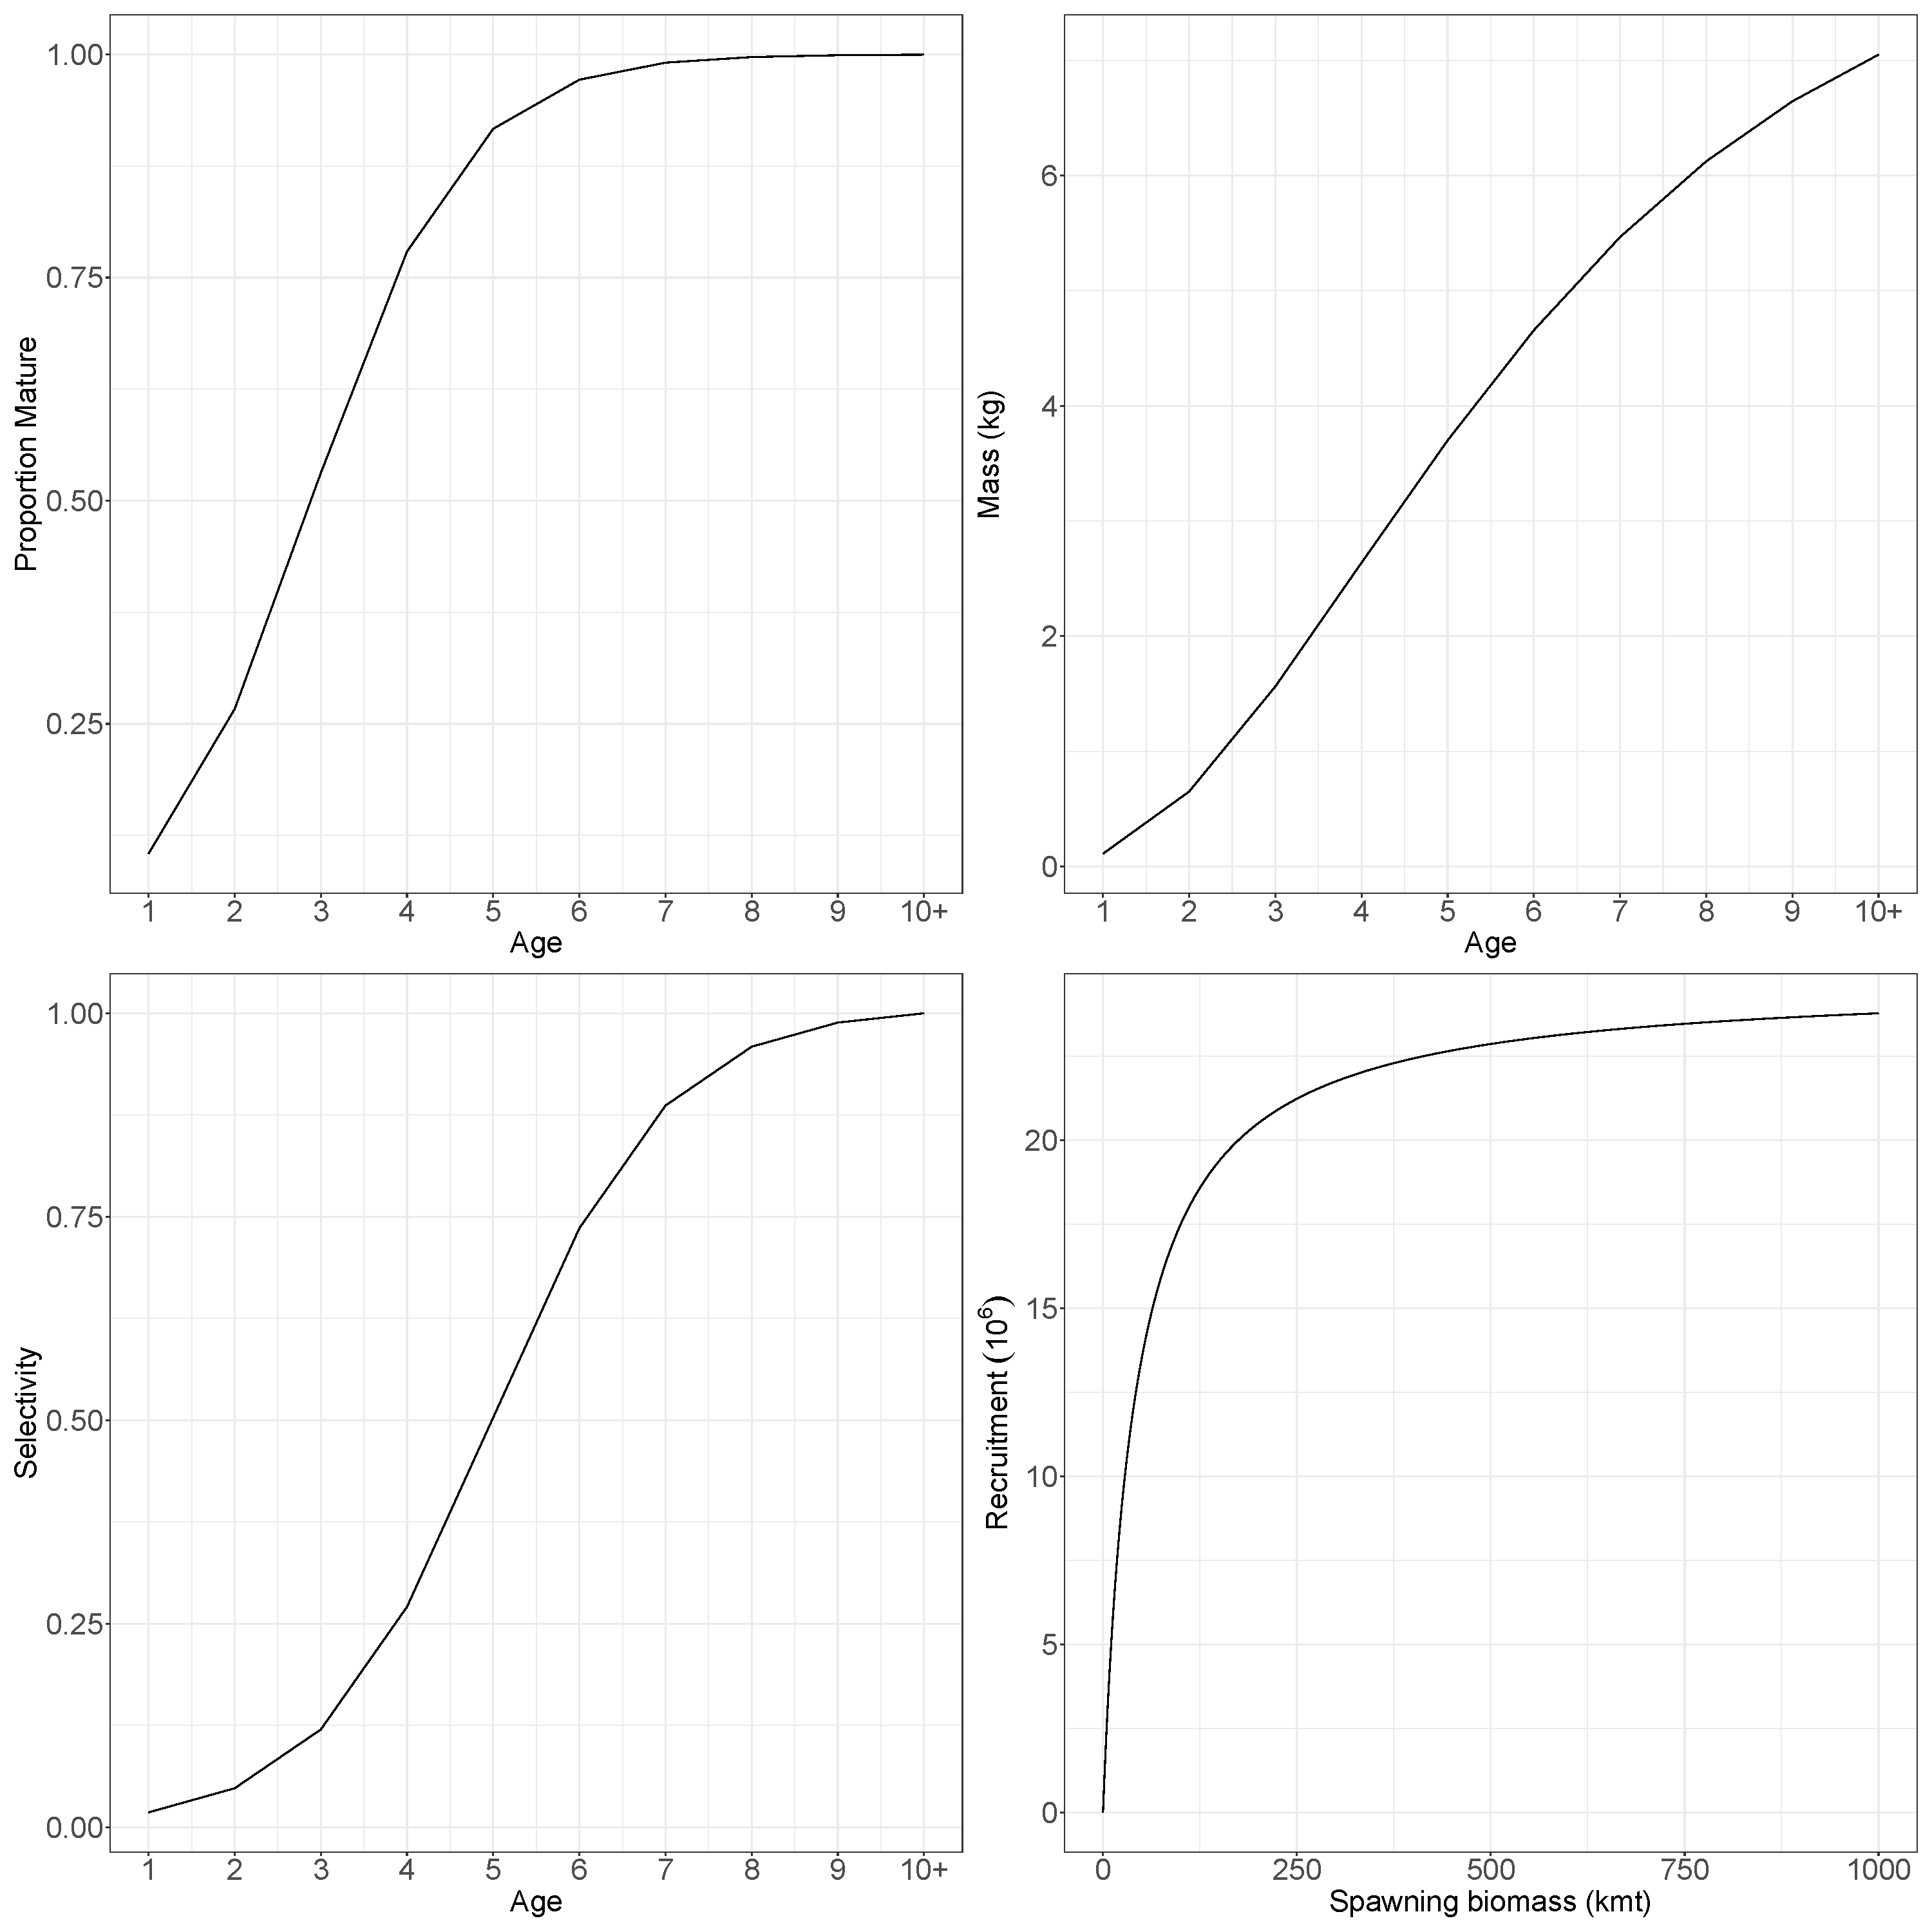
\includegraphics[width = \textwidth]{om_input_plots_figure}
\end{center}
\caption{The proportion mature at age, weight at age, fleet and index selectivity at age, and Beverton-Holt stock-recruit relationship assumed for the population in all operating models. For operating models with random effects on fleet selectivity, this represents the selectivity at the mean of the random effects.}\label{om_inputs_fig}
\end{figure}

\begin{landscape}
\begin{figure}
\caption{Example simulations of environmental covariate latent processes and observations with different levels of observation error, and different assumptions about variability of the latent process.}\label{om_ecov_example}
\begin{center}
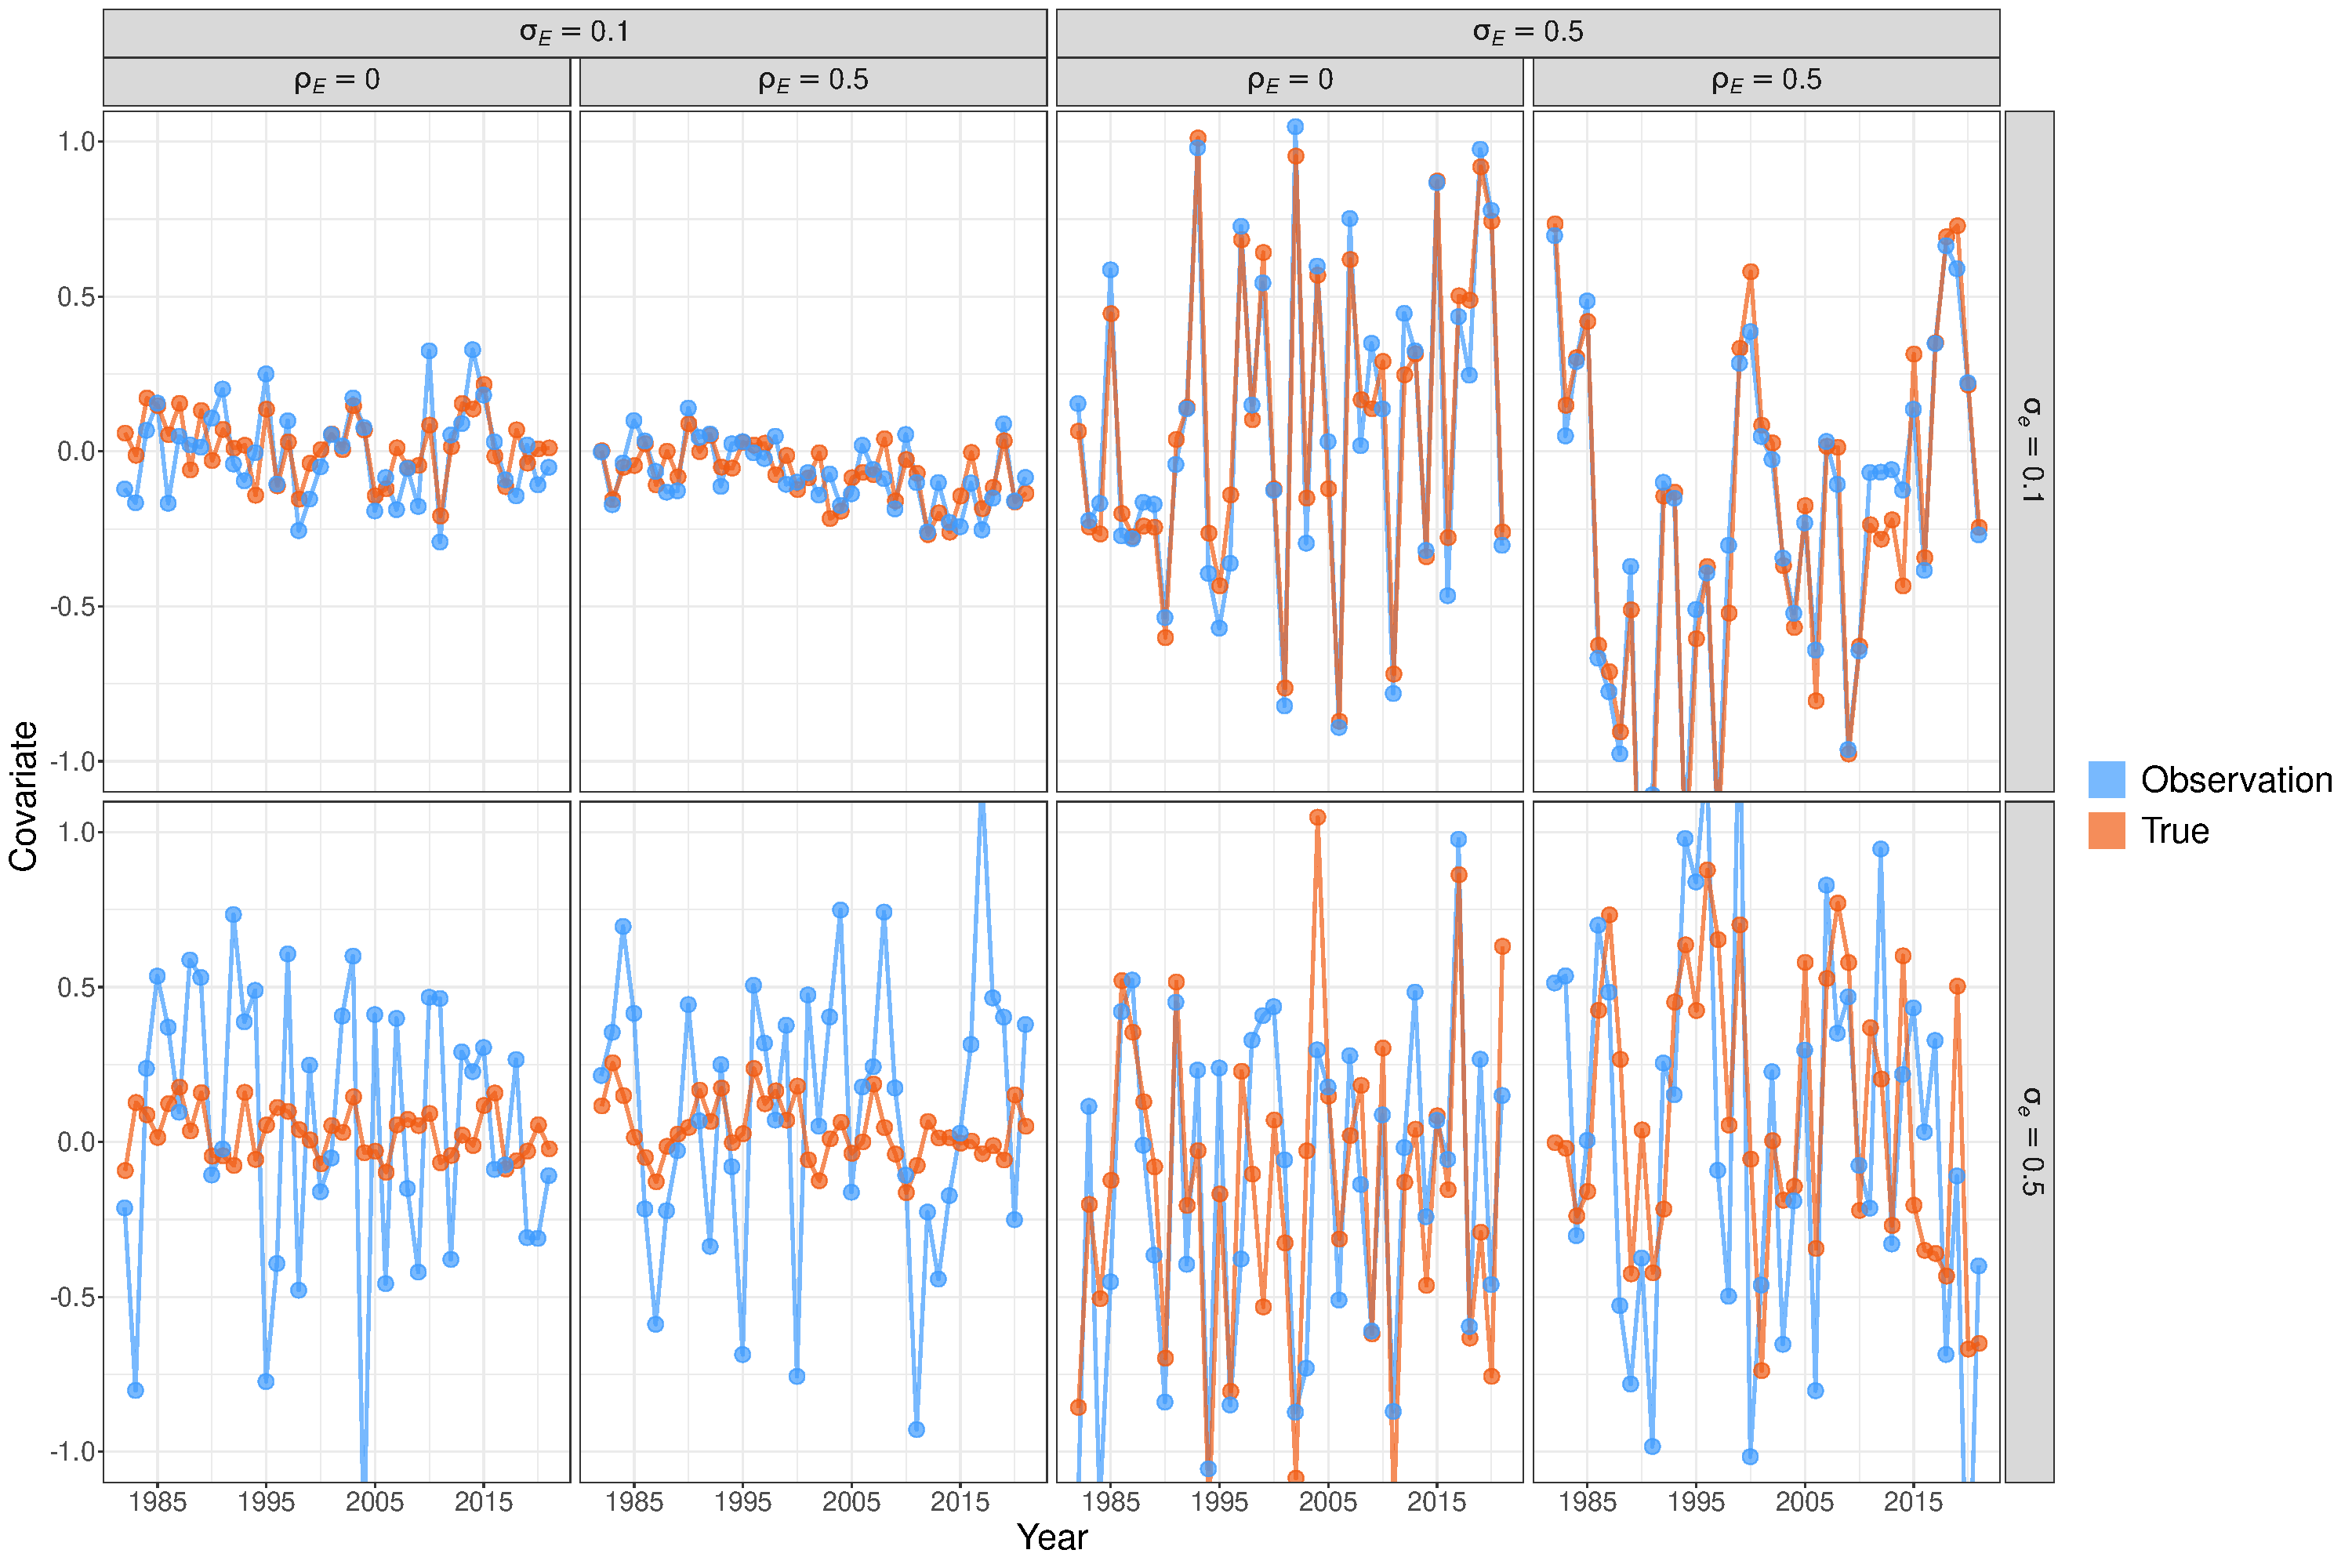
\includegraphics[height = \textheight]{Ecov_true_obs_example}
\end{center}
\end{figure}
\end{landscape}

\begin{landscape}
\begin{figure}
\caption{Example simulations of annual natural mortality rates that may be a function of a temporally varying environmental covariate and autoregressive random effects.}\label{M_example}
\begin{center}
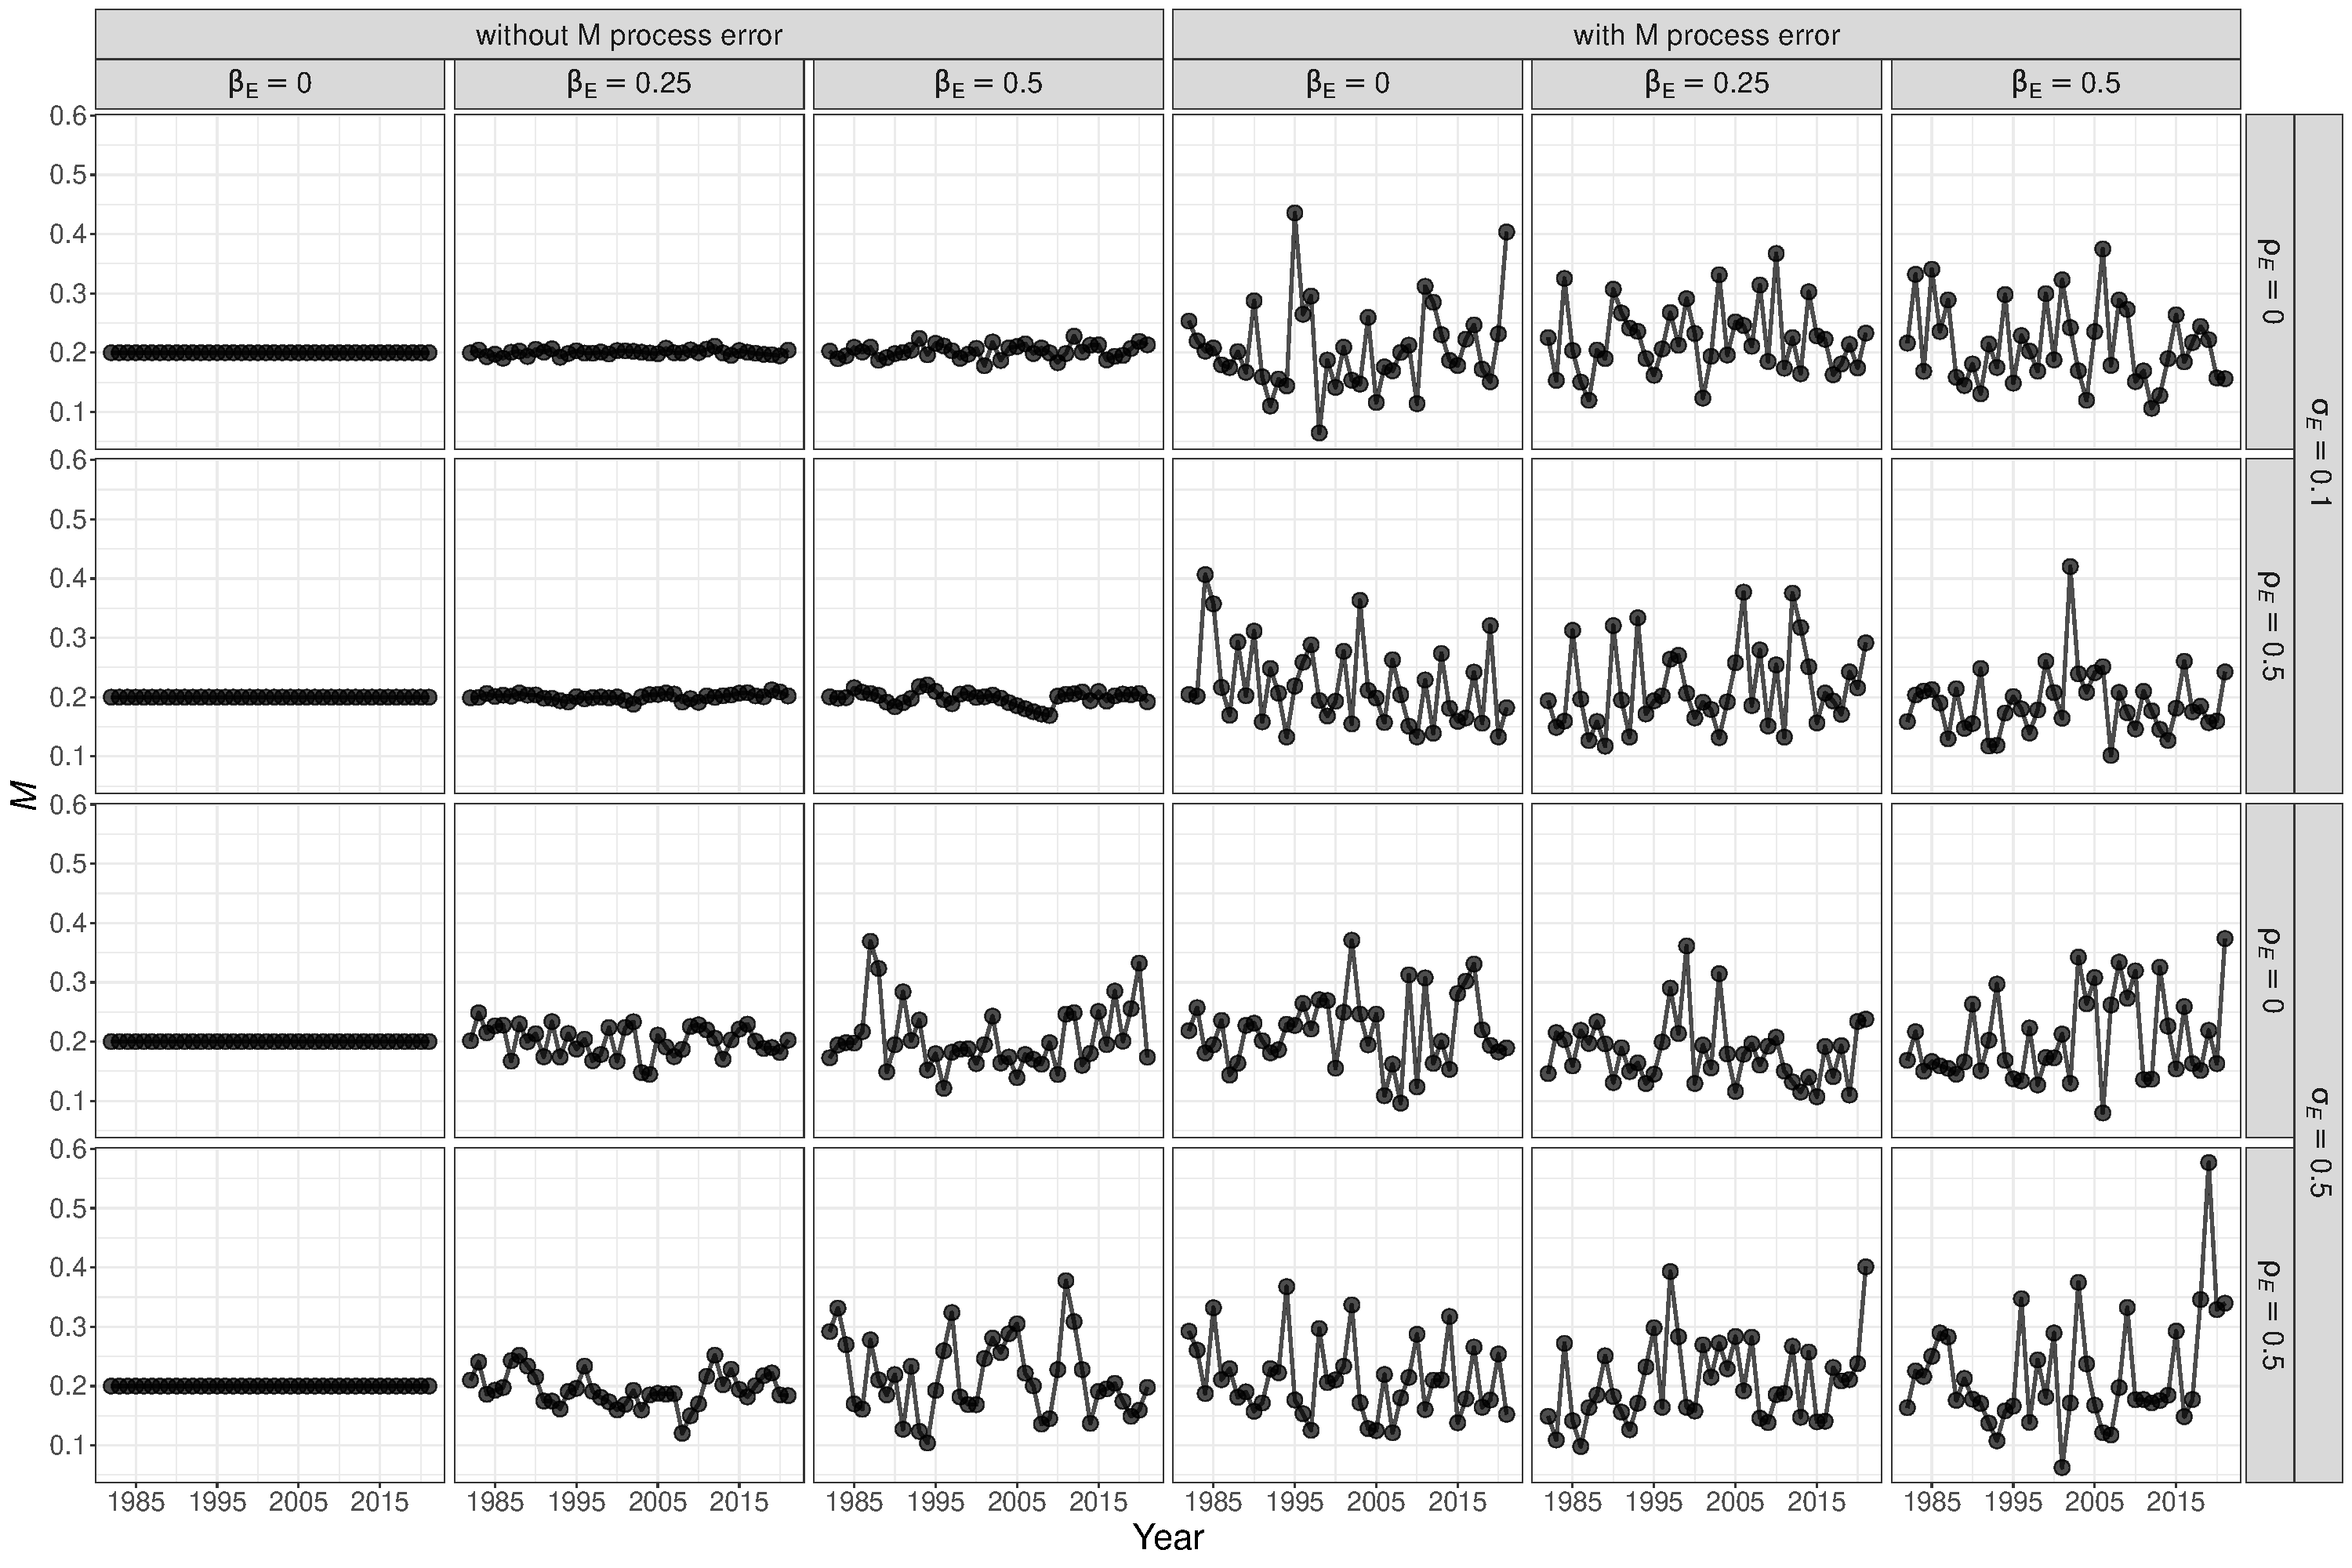
\includegraphics[height = \textheight]{M_example}
\end{center}
\end{figure}
\end{landscape}

\hypertarget{convergence-results}{%
\subsection*{Convergence results}\label{convergence-results}}
\addcontentsline{toc}{subsection}{Convergence results}

For R OMs, R EMs converged frequently except when there was contrast in fishing and covariate effects (\(\beta_E\)) were estimated and covariate observation uncertainty (\(\sigma_e\)) was high (Figure \ref{convergence_Rom}). There was little difference in convergence for R EMs whether median M was estimated or not. When R OMs had contrast in fishing, convergence of R+M EMs was generally better when the EM estimated median M, whereas in OMs with constant fishing, convergence was better when treating median M as known. Convergence of R+S EMs was generally worse than other process error configurations for R OMs, and there was no difference between EMs that estimated median M or not except when fishing pressure was constant where better convergence occurred when M was treated as known. Effects of true covariate effect size on convergence were apparent in some R OMs, but there did not appear to be any consistent patterns.

For R+S OMs, R+M EMs generally showed the worse probability of convergence that EMs with R and R+S configurations (Figure \ref{convergence_RSom}). Convergence probability was high for all R and R+S EMs when covariate observation uncertainty was low. Although probability of convergence was generally greater when covariate effects were not estimated, there were no strong trends in convergence for any of the EMS with increased true effect size.

For R+M OMs, R+S EMs generally converged less frequently than those with R and R+M configurations (Figure \ref{convergence_RMom}). Convergence probability for R OMs was generally the greatest of the three process error configurations. As with R+S OMs, there were no strong trends in convergence for any of the EMS with increased true covariate effect size. However, there was also not strong effects of estimating the covariate effect on convergence except for some OMs with higher covariate observation uncertainty. Like R OMs, when R+M OMs had contrast in fishing, convergence of R+M EMs was generally better when the EM estimated median M and the convergence was better when treating median M as known when the OM had constant fishing.

\begin{landscape}
\begin{figure}
\begin{center}
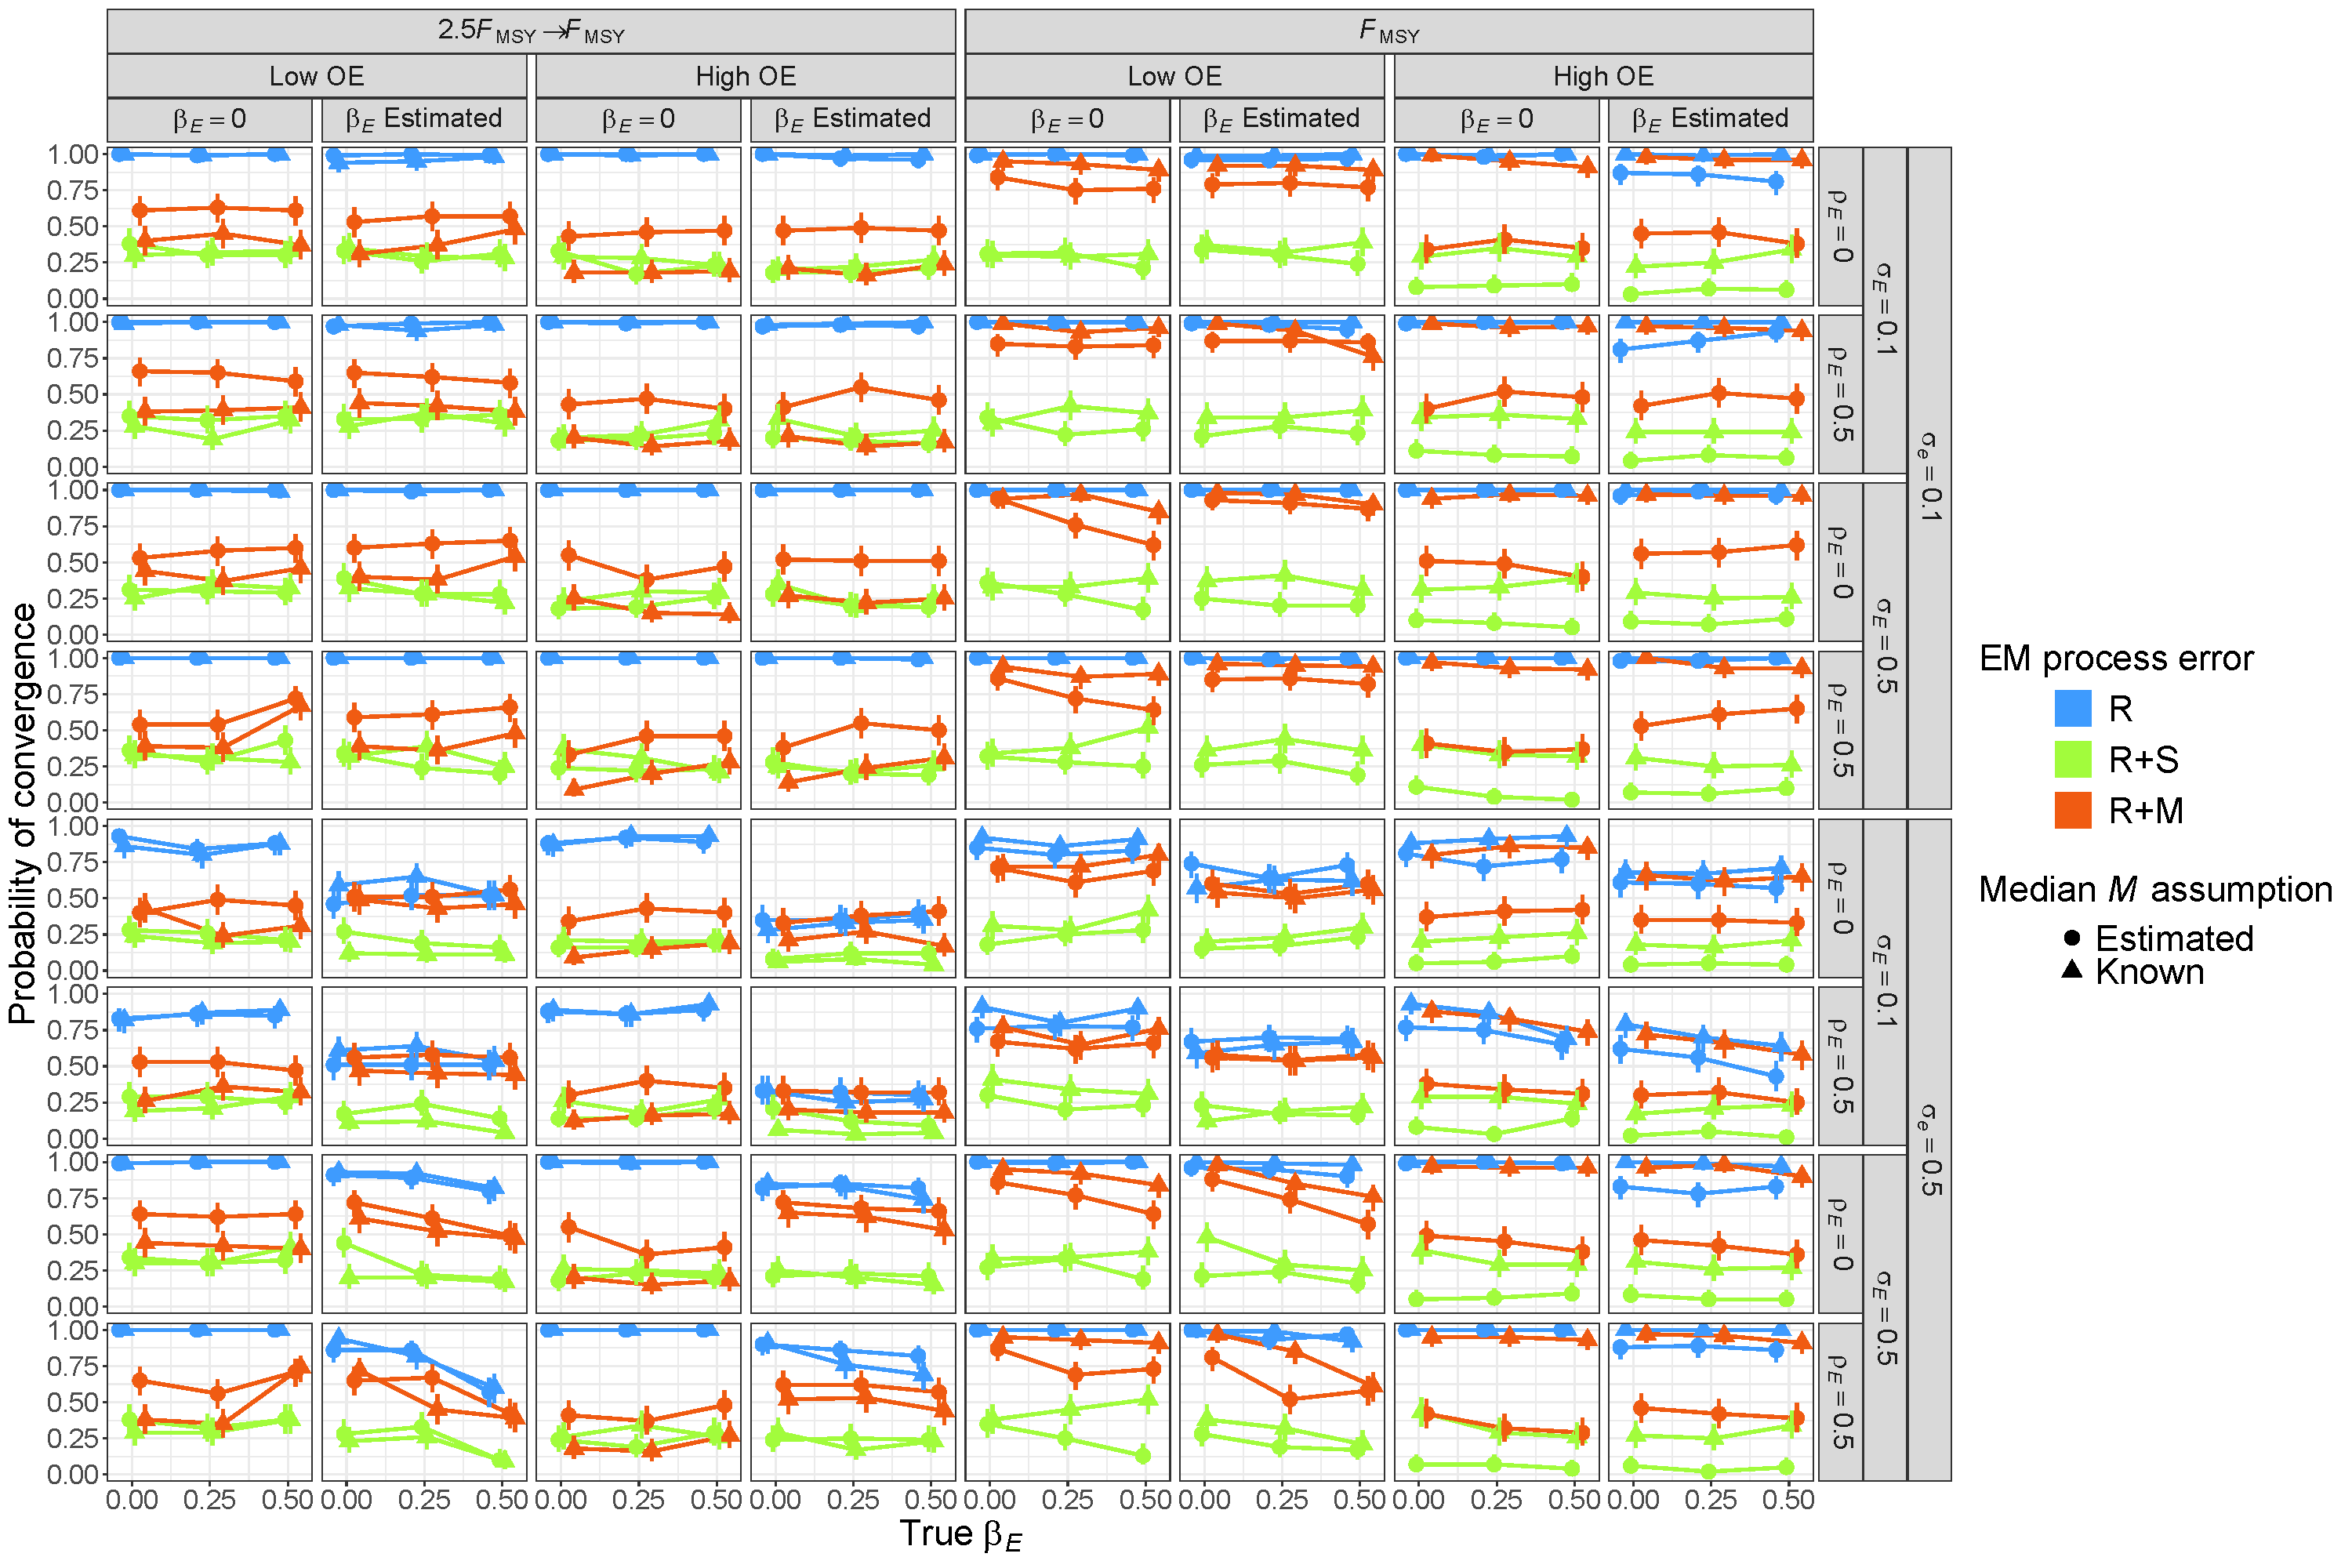
\includegraphics{convergence_Rom}
\end{center}
\caption{Estimated probability of fits providing Hessian-based standard errors for EMs assuming alternative process error, that estimate or assume known median natural mortality, and that estimate or assume no covariate effect on median natural mortality when fitted to R OMs and three levels of true covariate effect on median natural mortality (x axis). Vertical lines represent 95\% confidence intervals.}\label{convergence_Rom}
\end{figure}
\end{landscape}

\begin{landscape}
\begin{figure}
\begin{center}
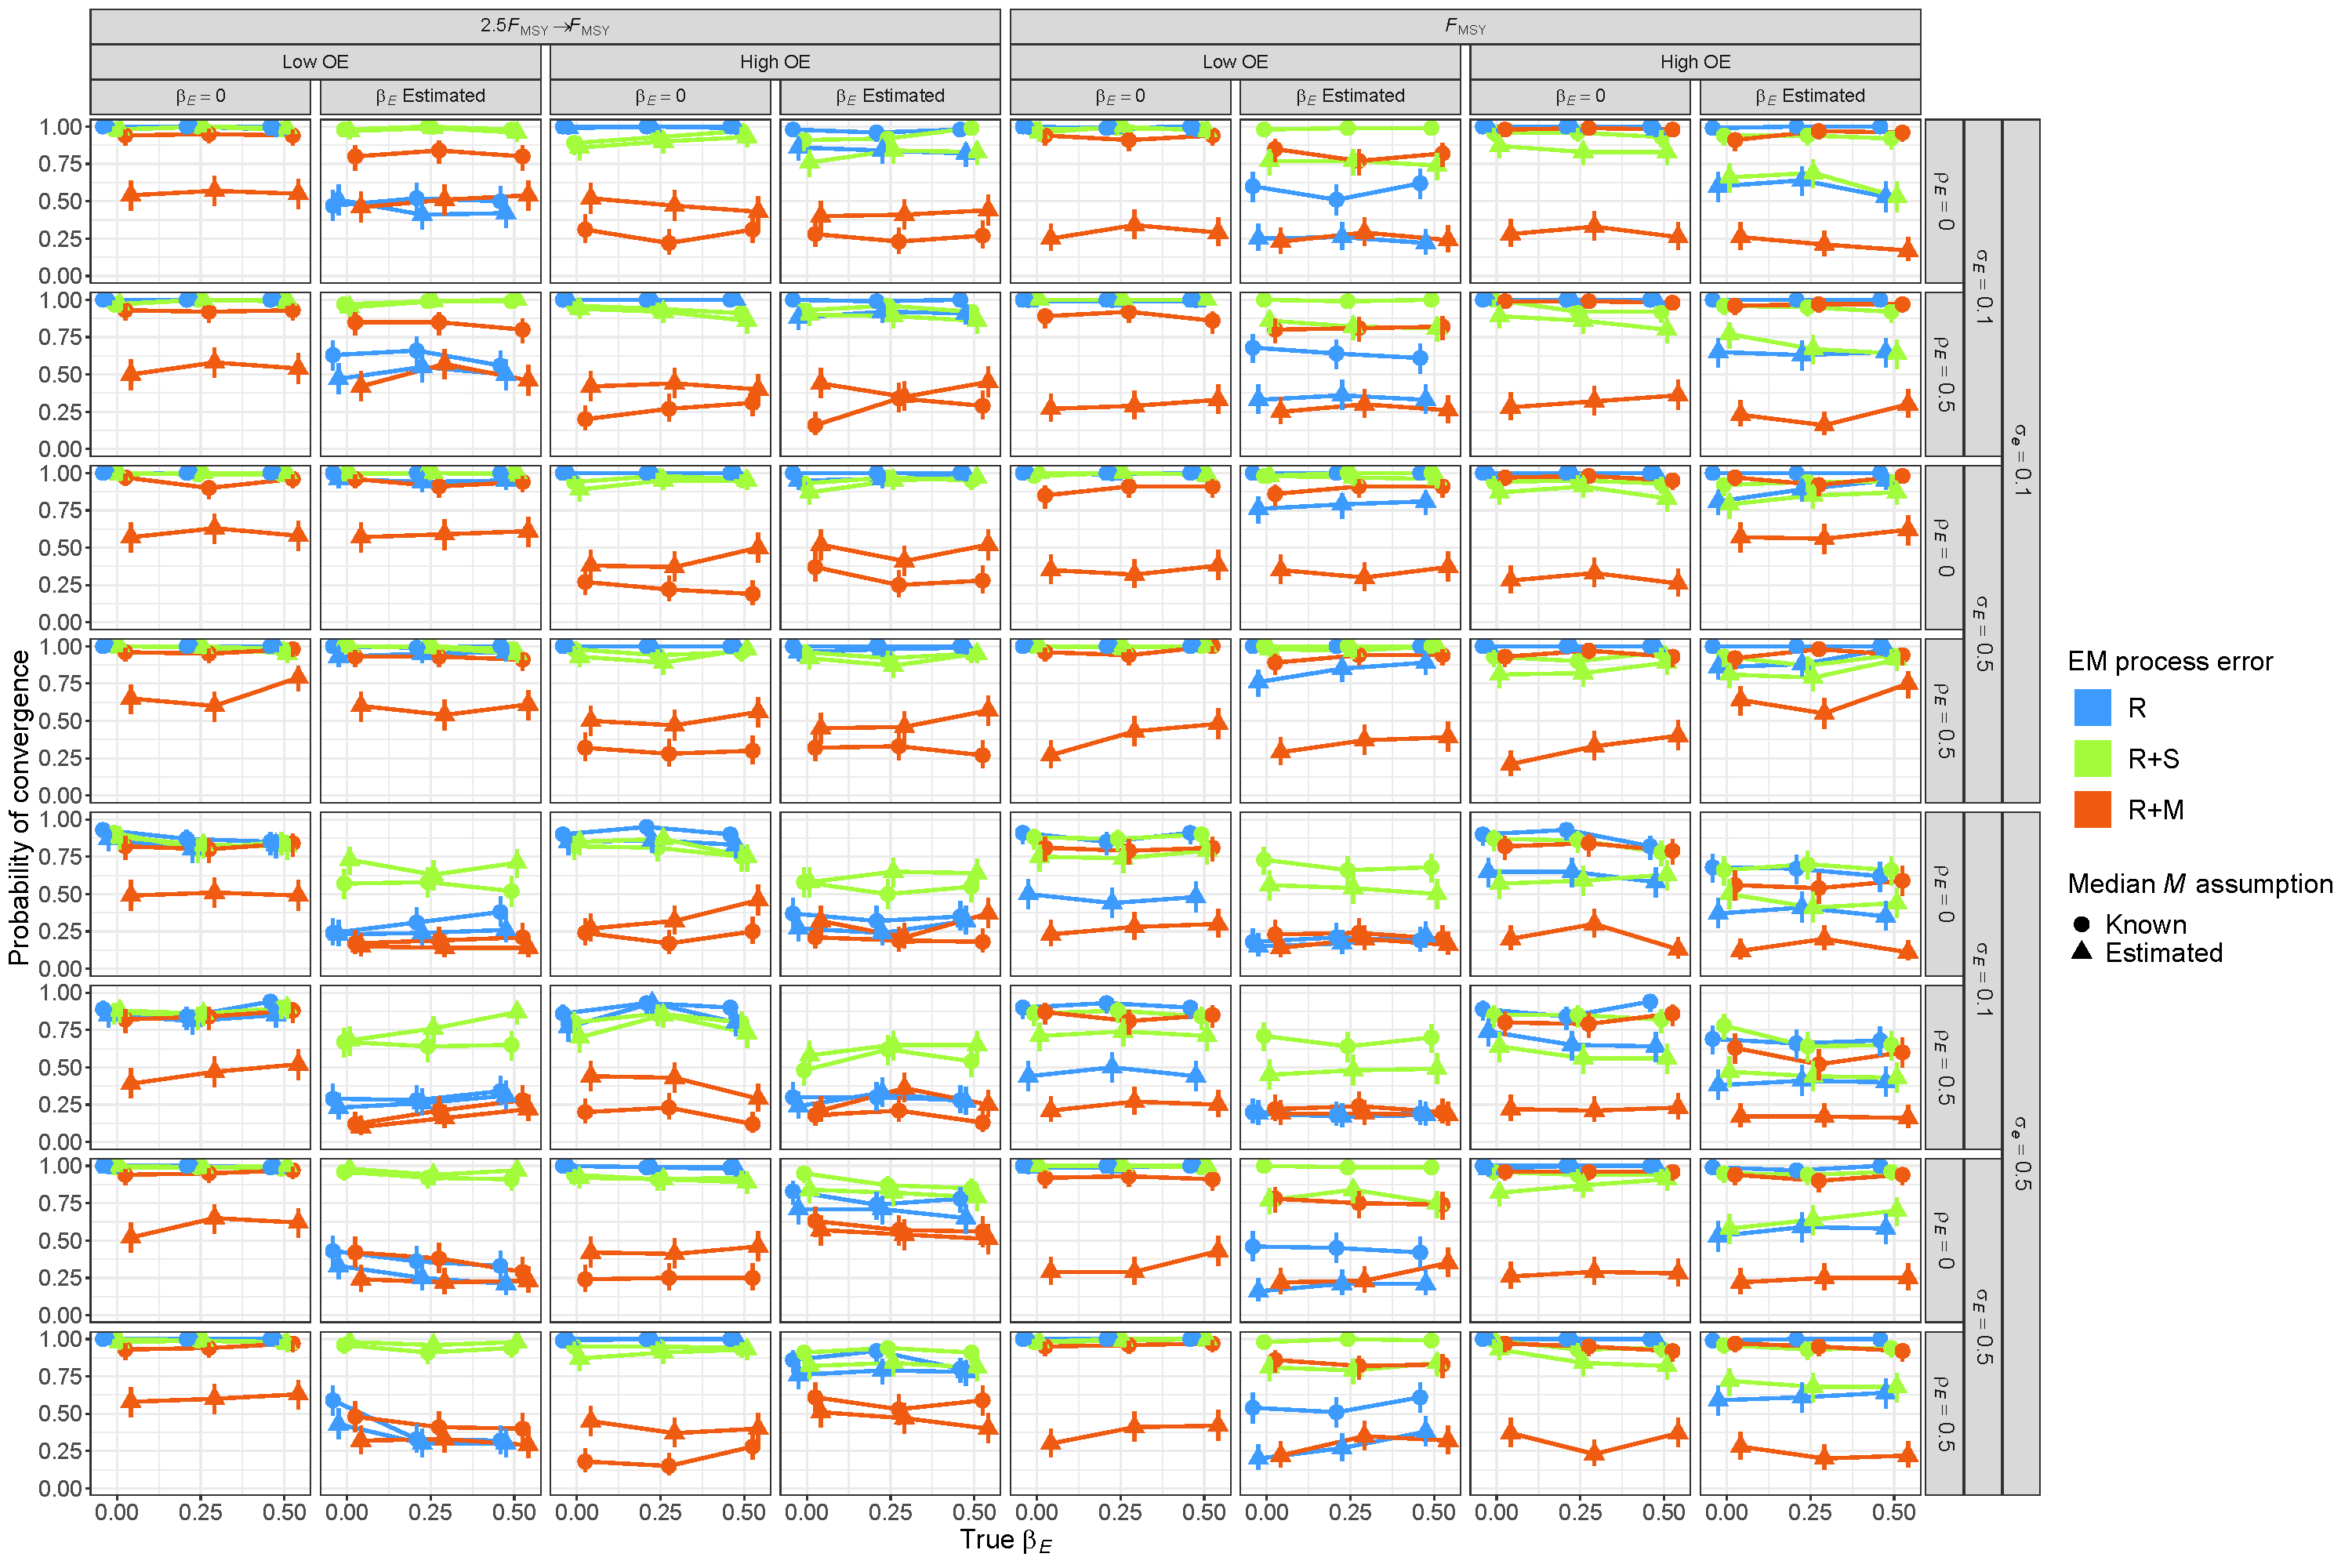
\includegraphics{convergence_RSom}
\end{center}
\caption{Estimated probability of fits providing Hessian-based standard errors for EMs assuming alternative process error, that estimate or assume known median natural mortality, and that estimate or assume no covariate effect on median natural mortality when fitted to R+S OMs and three levels of true covariate effect on median natural mortality (x axis). Vertical lines represent 95\% confidence intervals.}\label{convergence_RSom}
\end{figure}
\end{landscape}

\begin{landscape}
\begin{figure}
\begin{center}
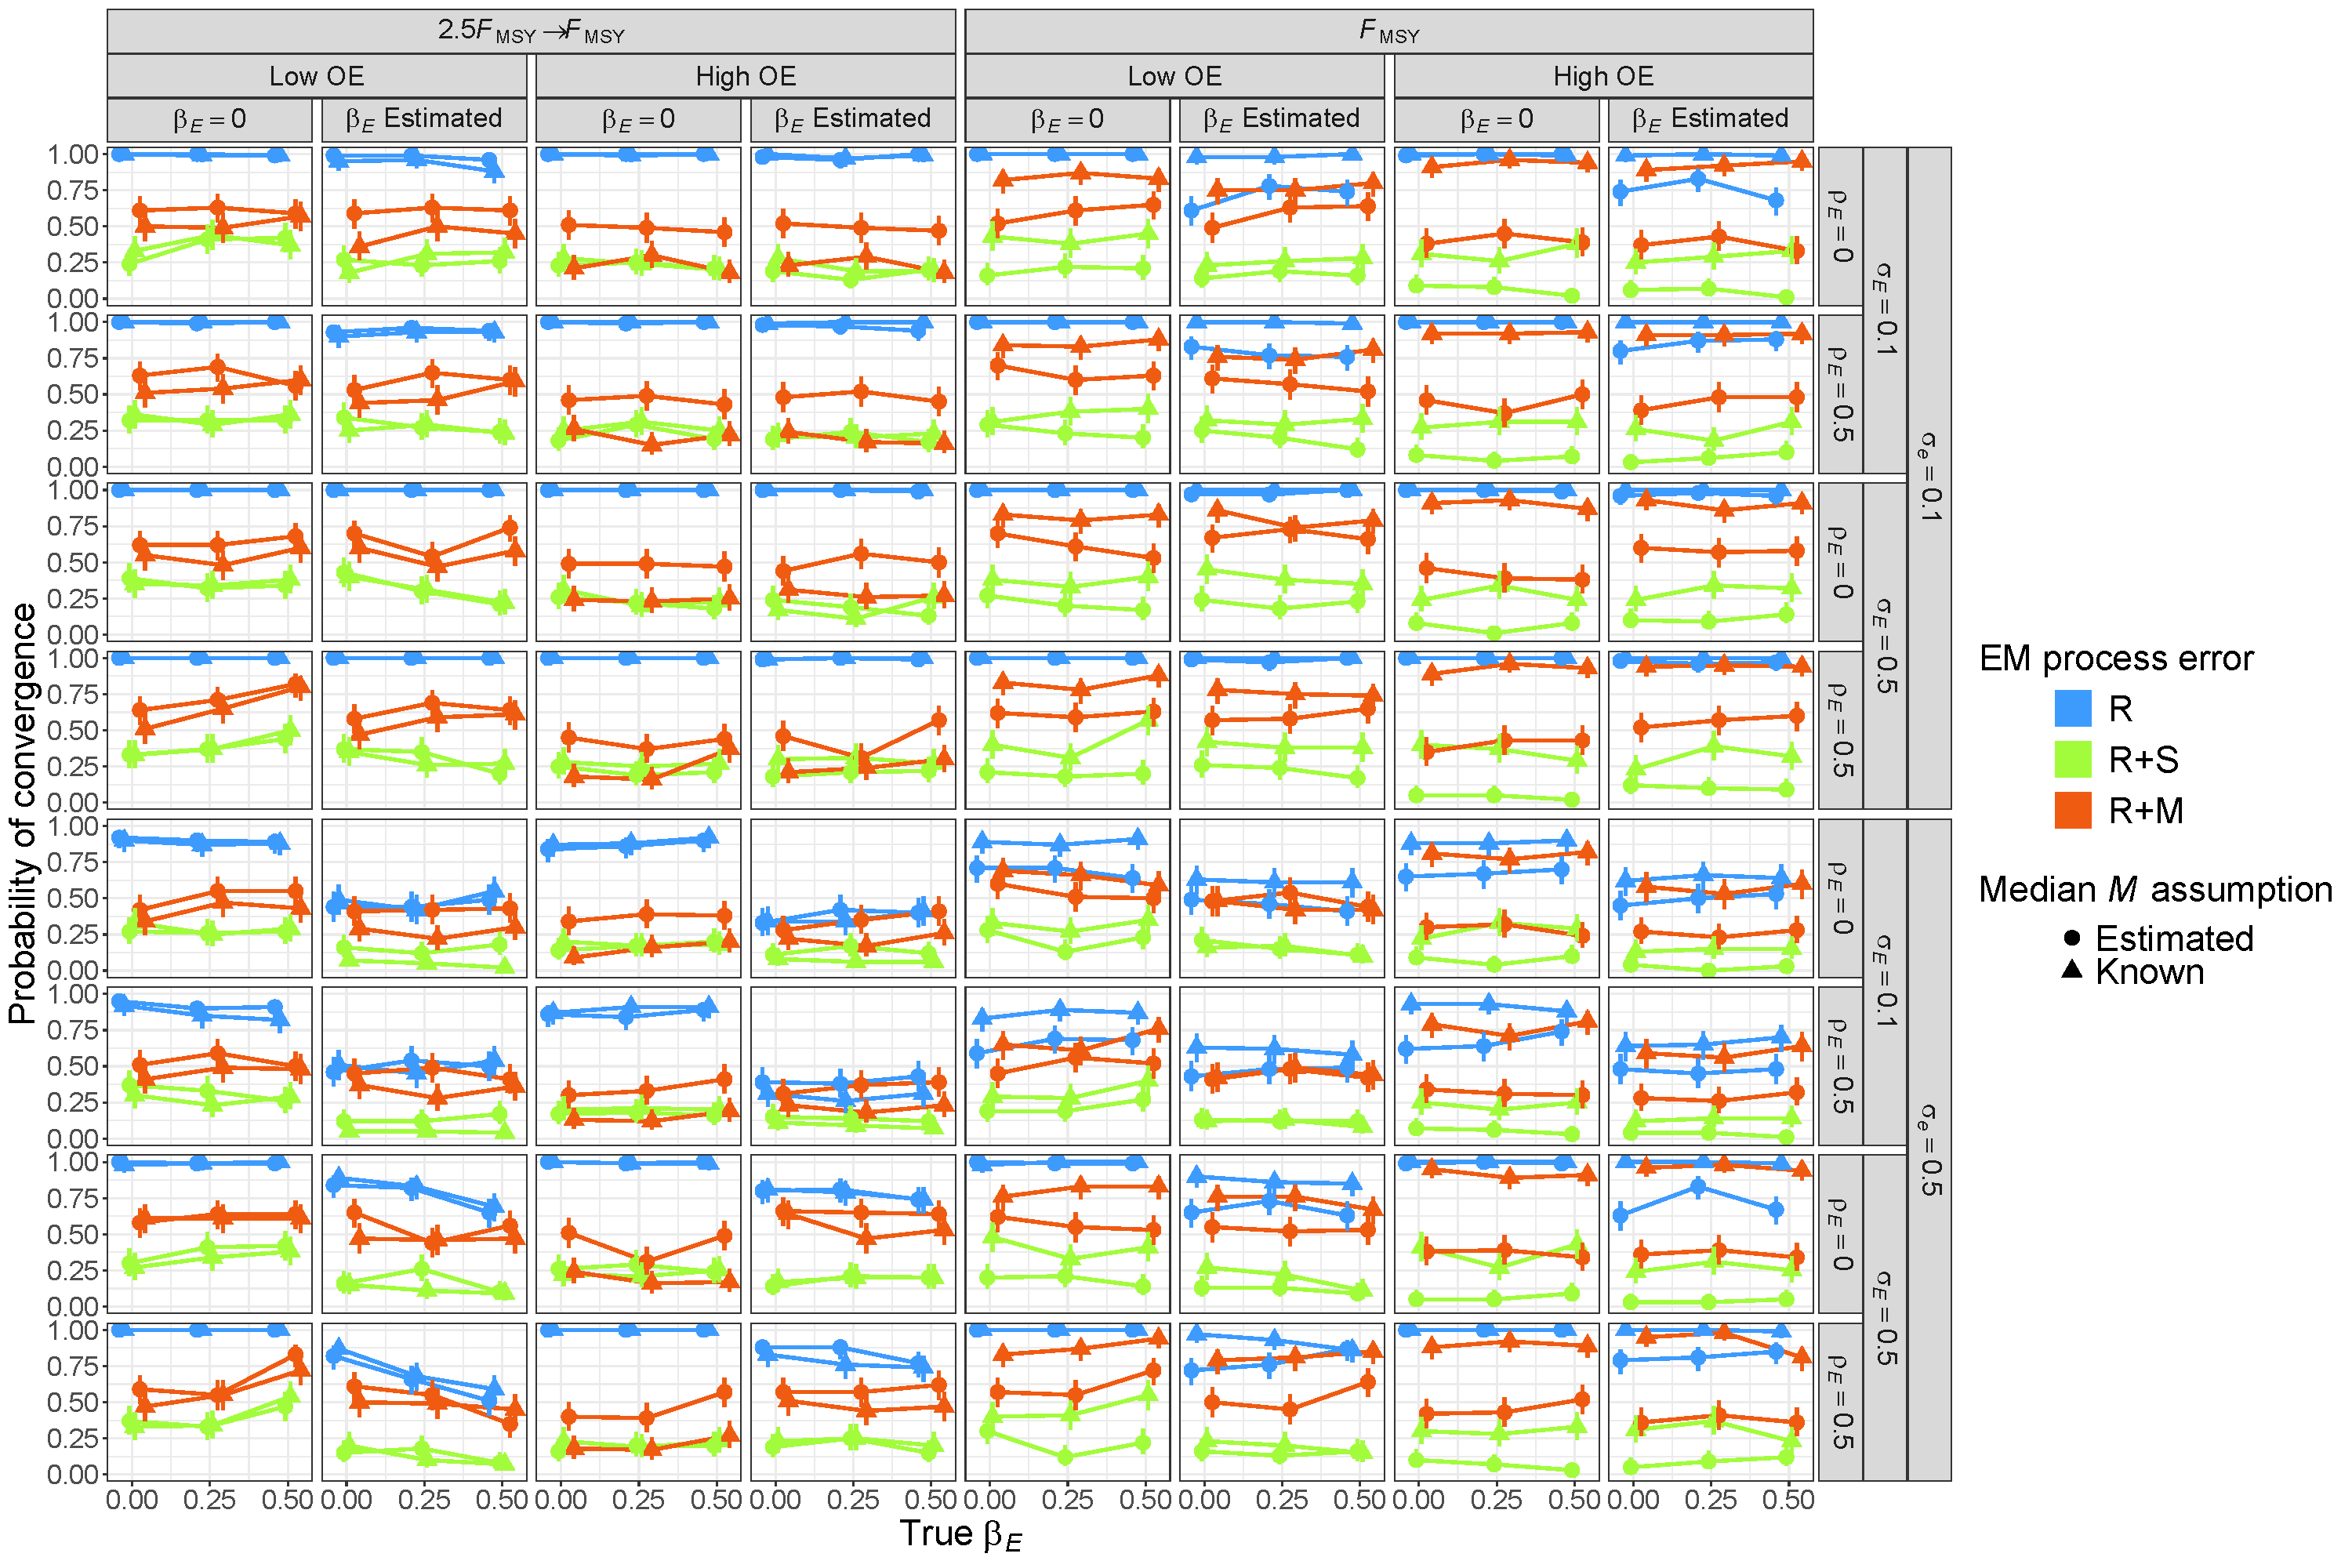
\includegraphics{convergence_RMom}
\end{center}
\caption{Estimated probability of fits providing Hessian-based standard errors for EMs assuming alternative process error, that estimate or assume known median natural mortality, and that estimate or assume no covariate effect on median natural mortality when fitted to R+M OMs and three levels of true covariate effect on median natural mortality (x axis). Vertical lines represent 95\% confidence intervals.}\label{convergence_RMom}
\end{figure}
\end{landscape}

\hypertarget{aic-results}{%
\subsection*{AIC results}\label{aic-results}}
\addcontentsline{toc}{subsection}{AIC results}

\begin{landscape}
\begin{figure}
\begin{center}
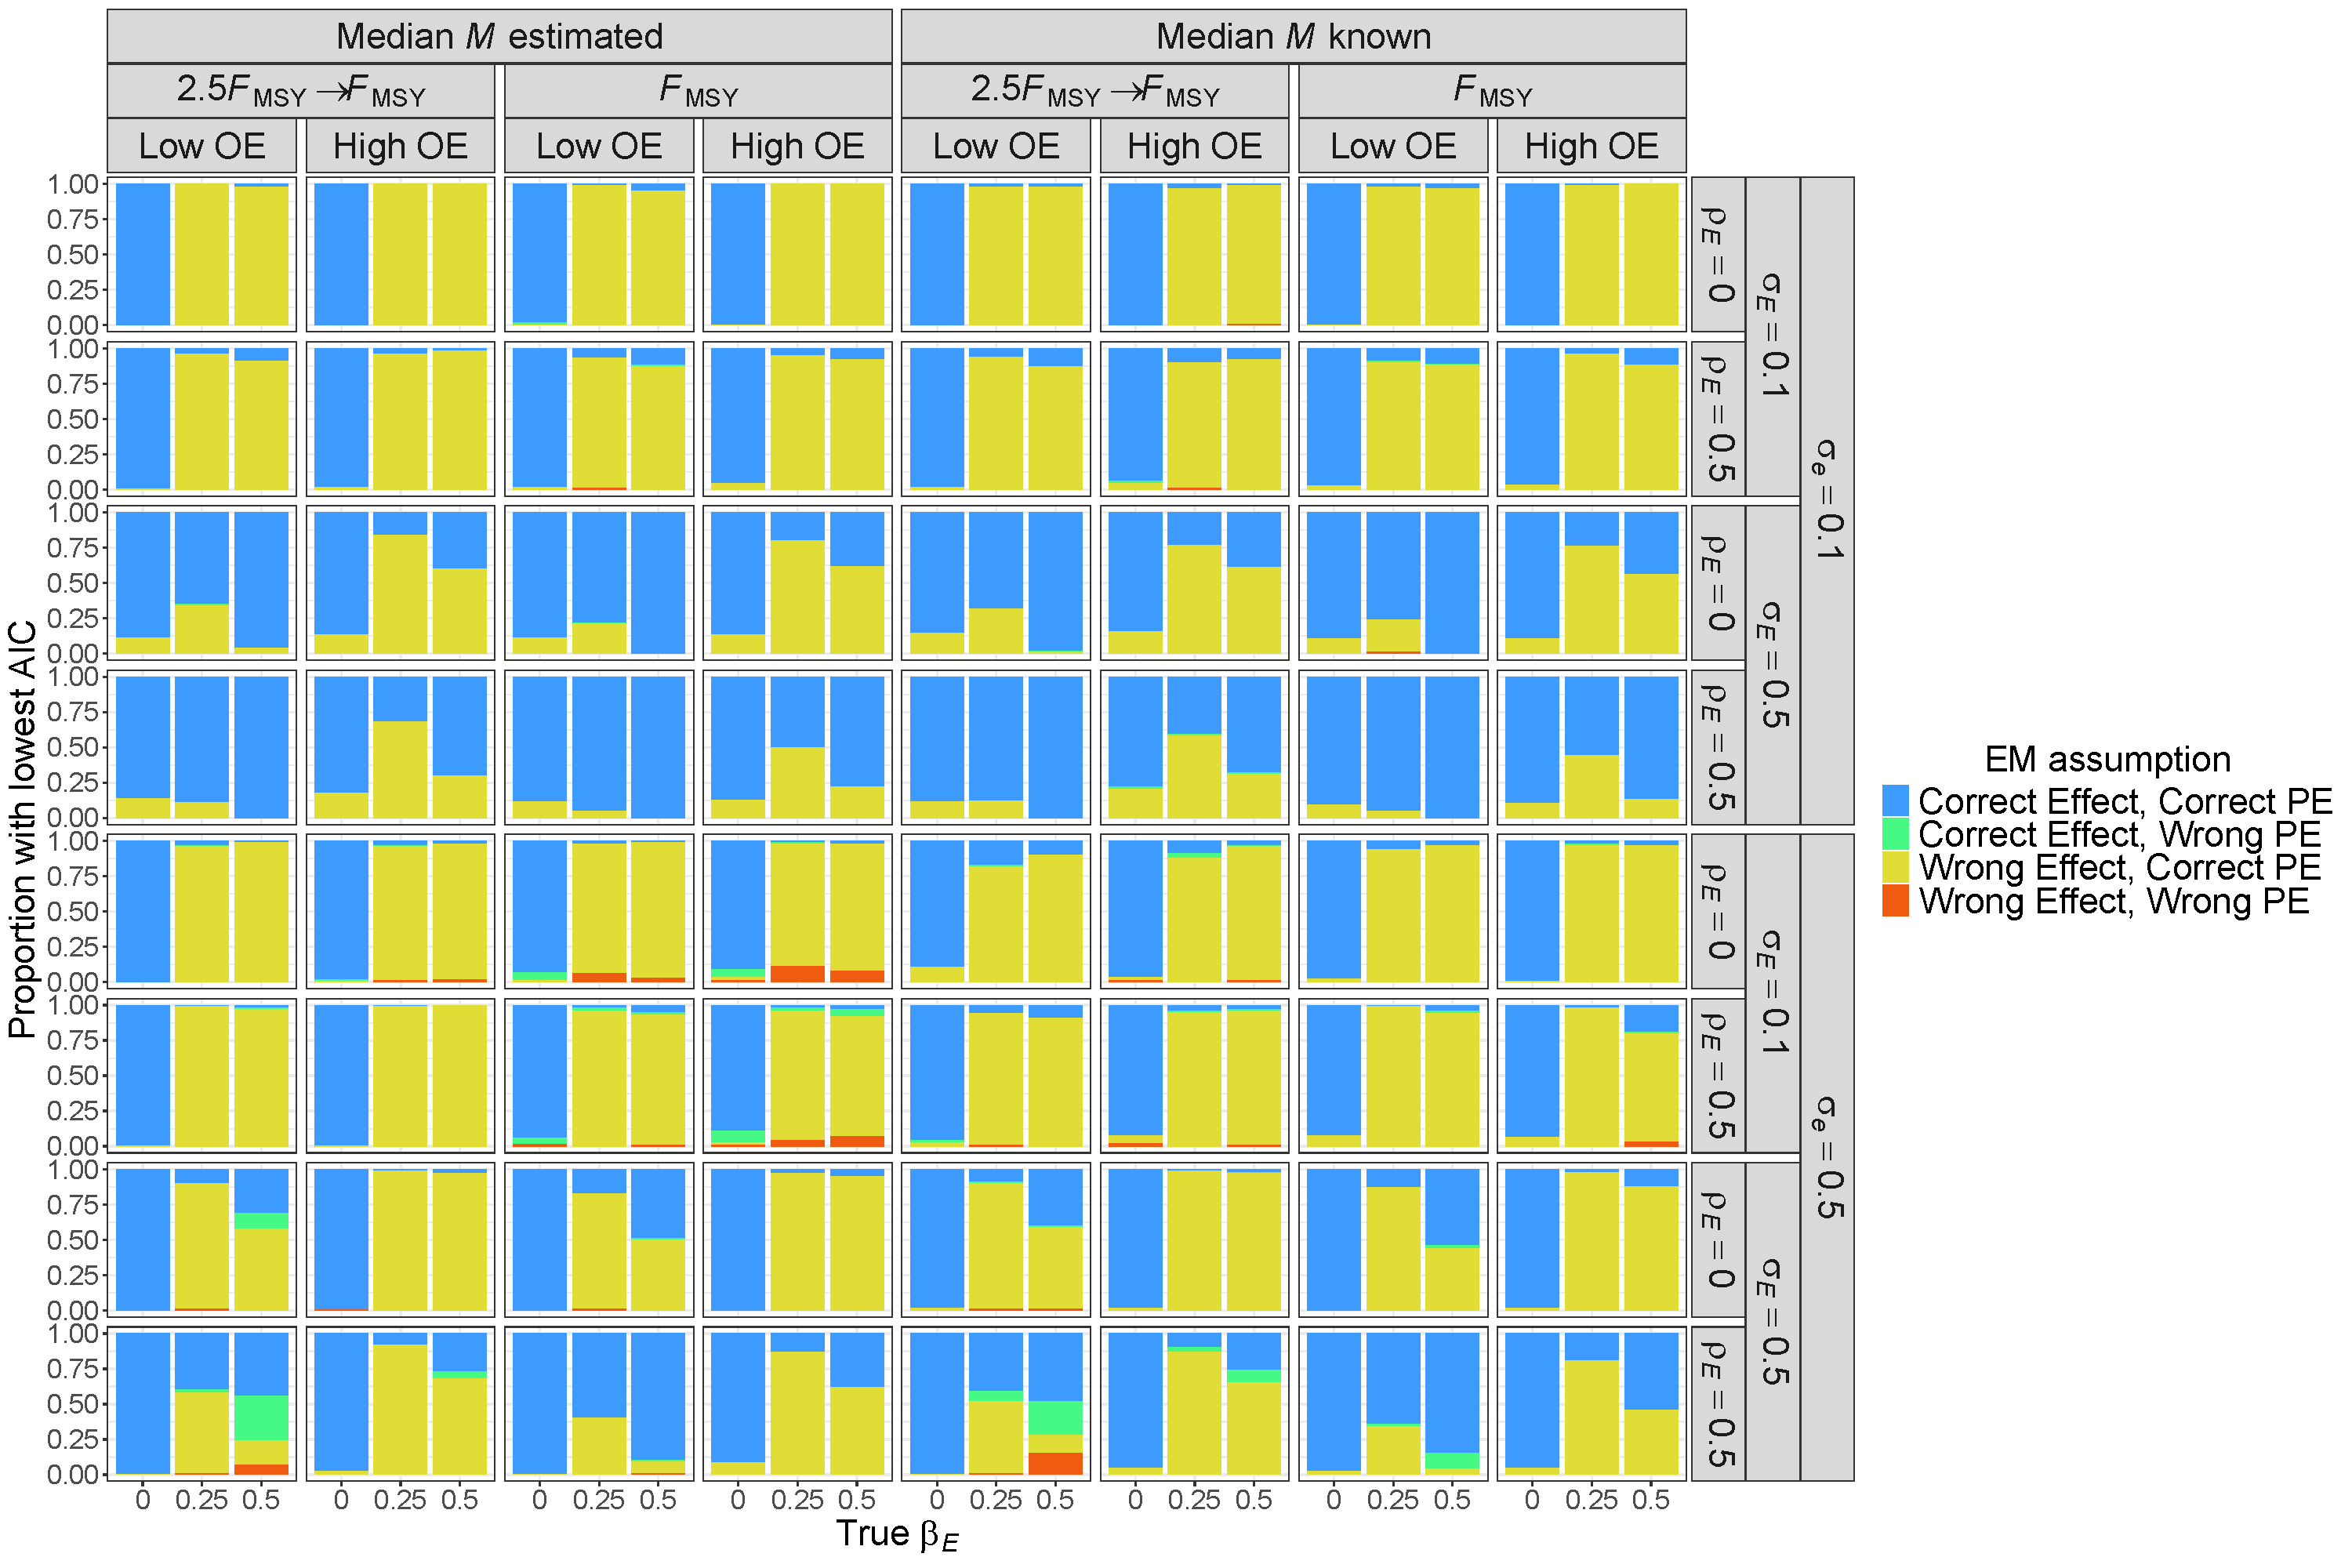
\includegraphics[height = \textheight]{aic_Rom}
\end{center}
\caption{Proportion of simulated data sets for R OMs where the EM type (treatment of environmental covariate and assumed process error type) had the lowest AIC.}\label{aic_Rom}
\end{figure}
\end{landscape}

\begin{landscape}
\begin{figure}
\begin{center}
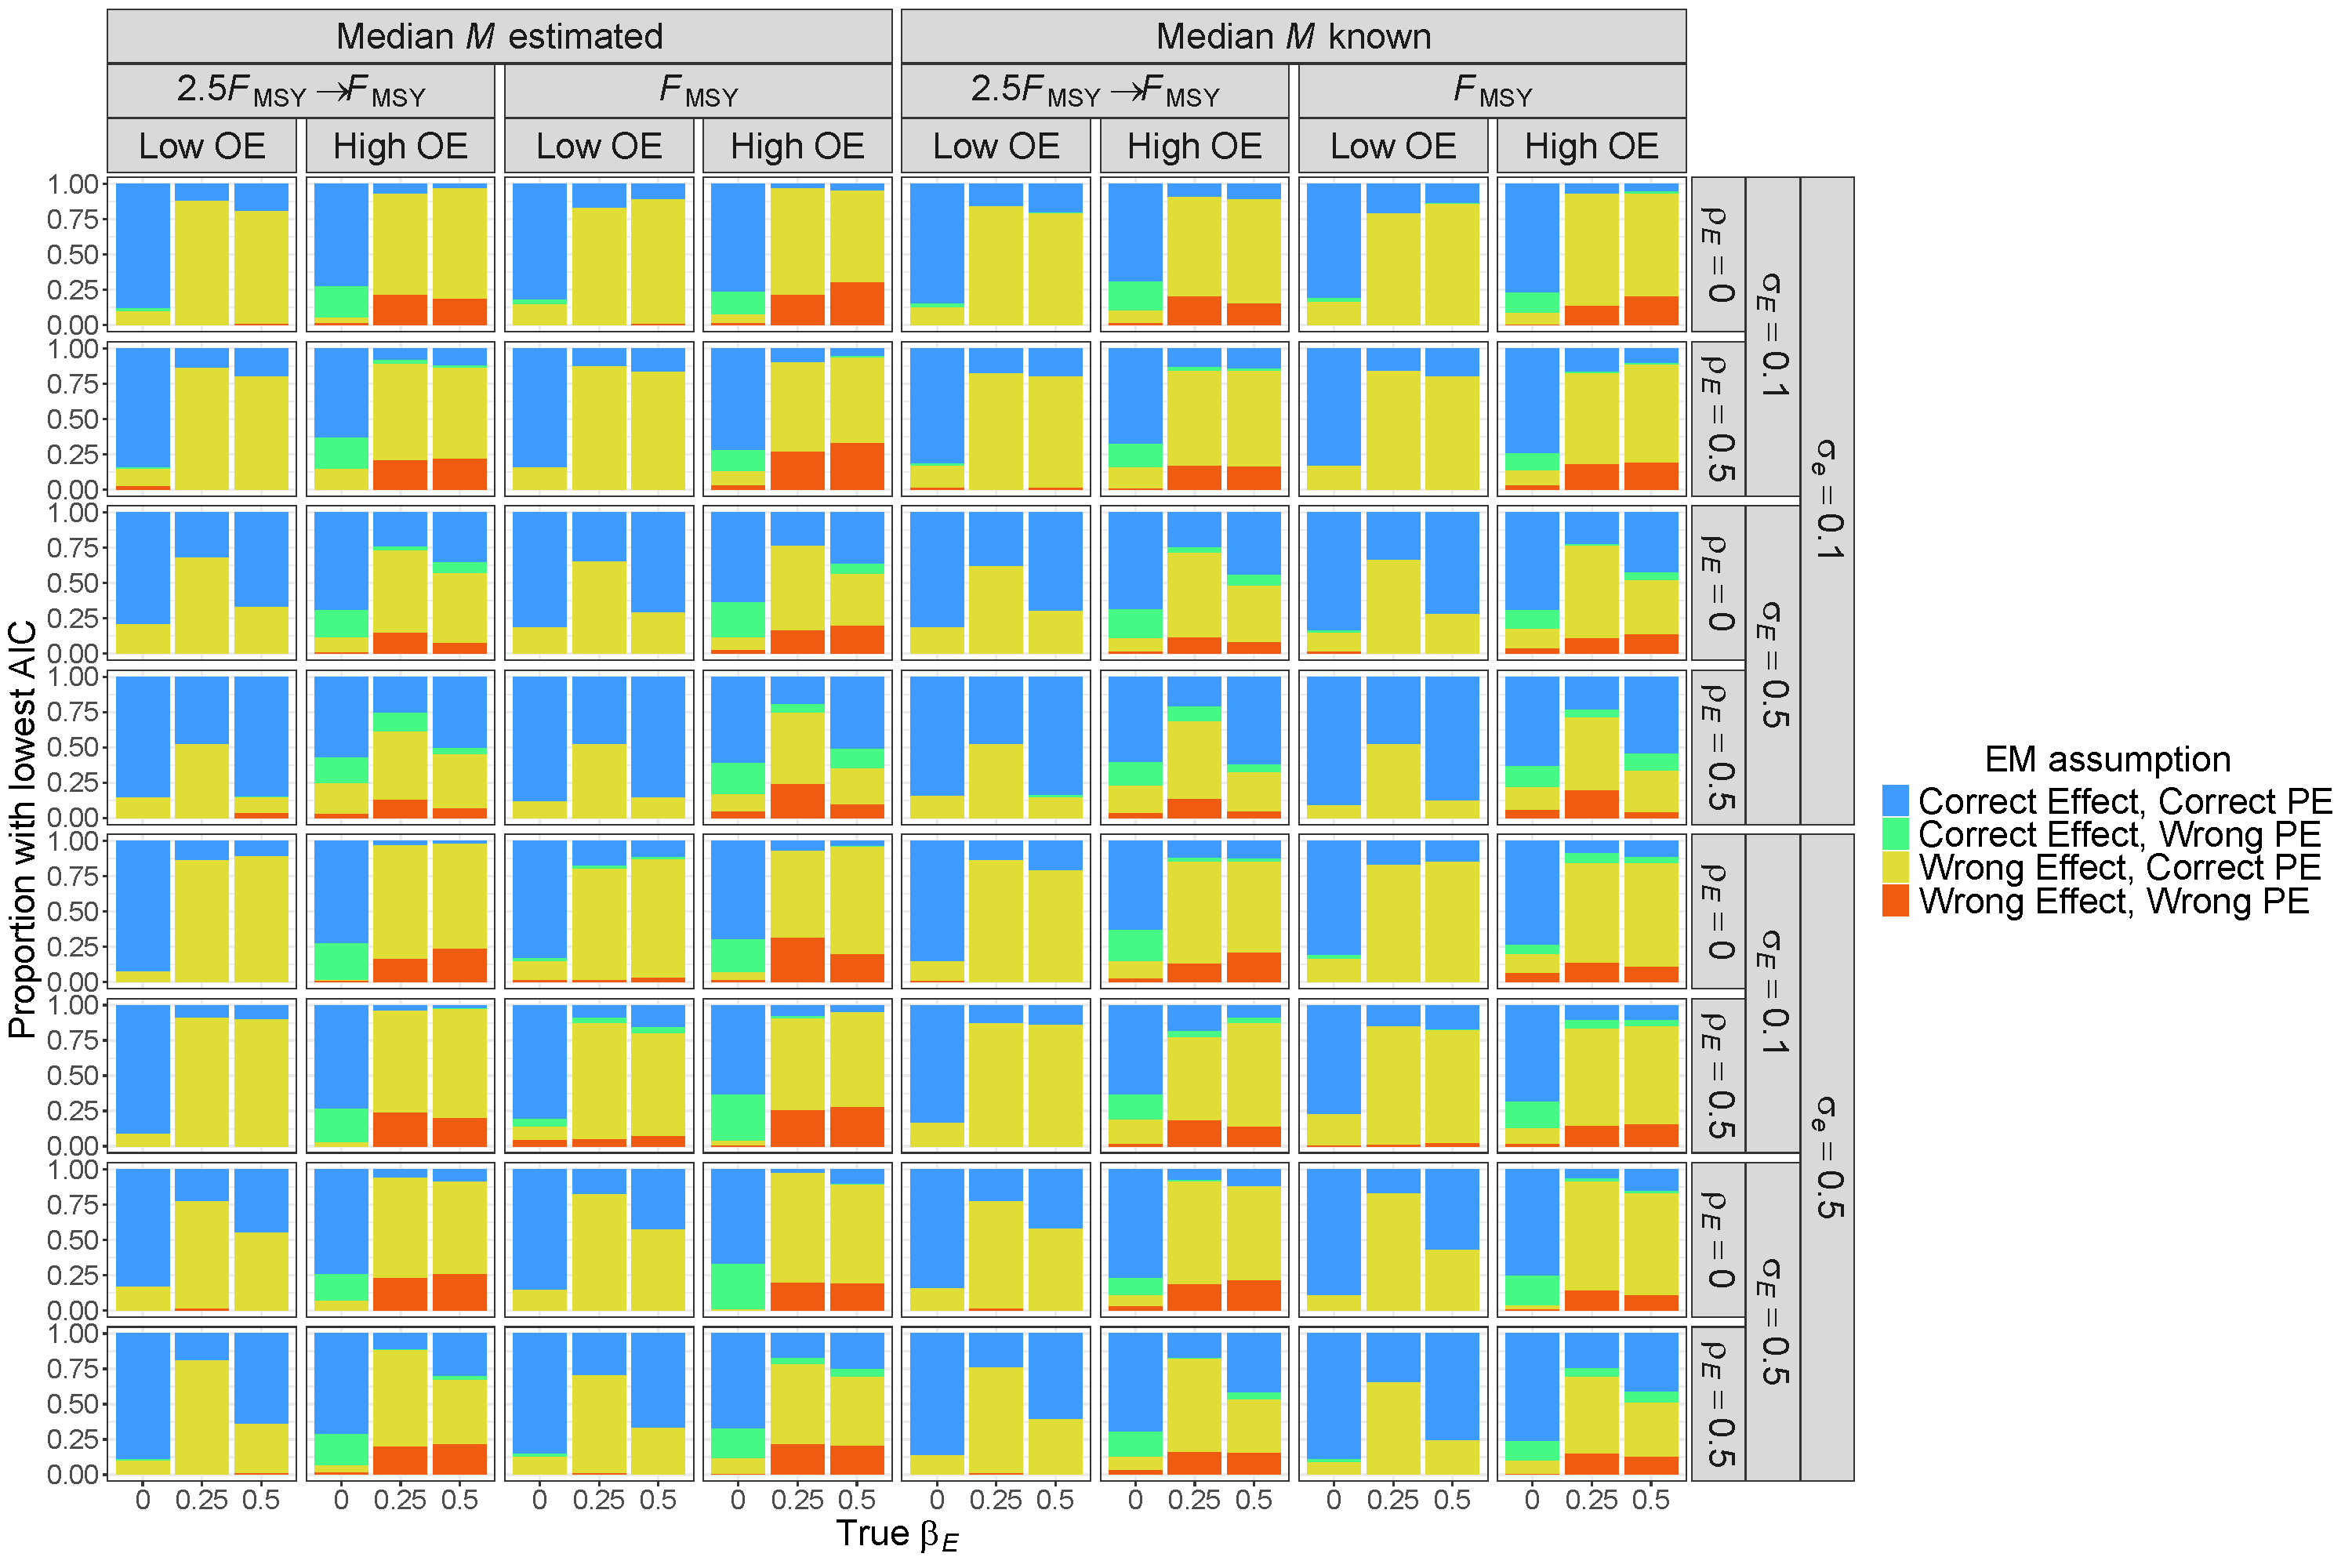
\includegraphics[height = \textheight]{aic_RSom}
\end{center}
\caption{Proportion of simulated data sets for R+S OMs where the EM type (treatment of environmental covariate and assumed process error type) had the lowest AIC.}\label{aic_RSom}
\end{figure}
\end{landscape}

\begin{landscape}
\begin{figure}
\begin{center}
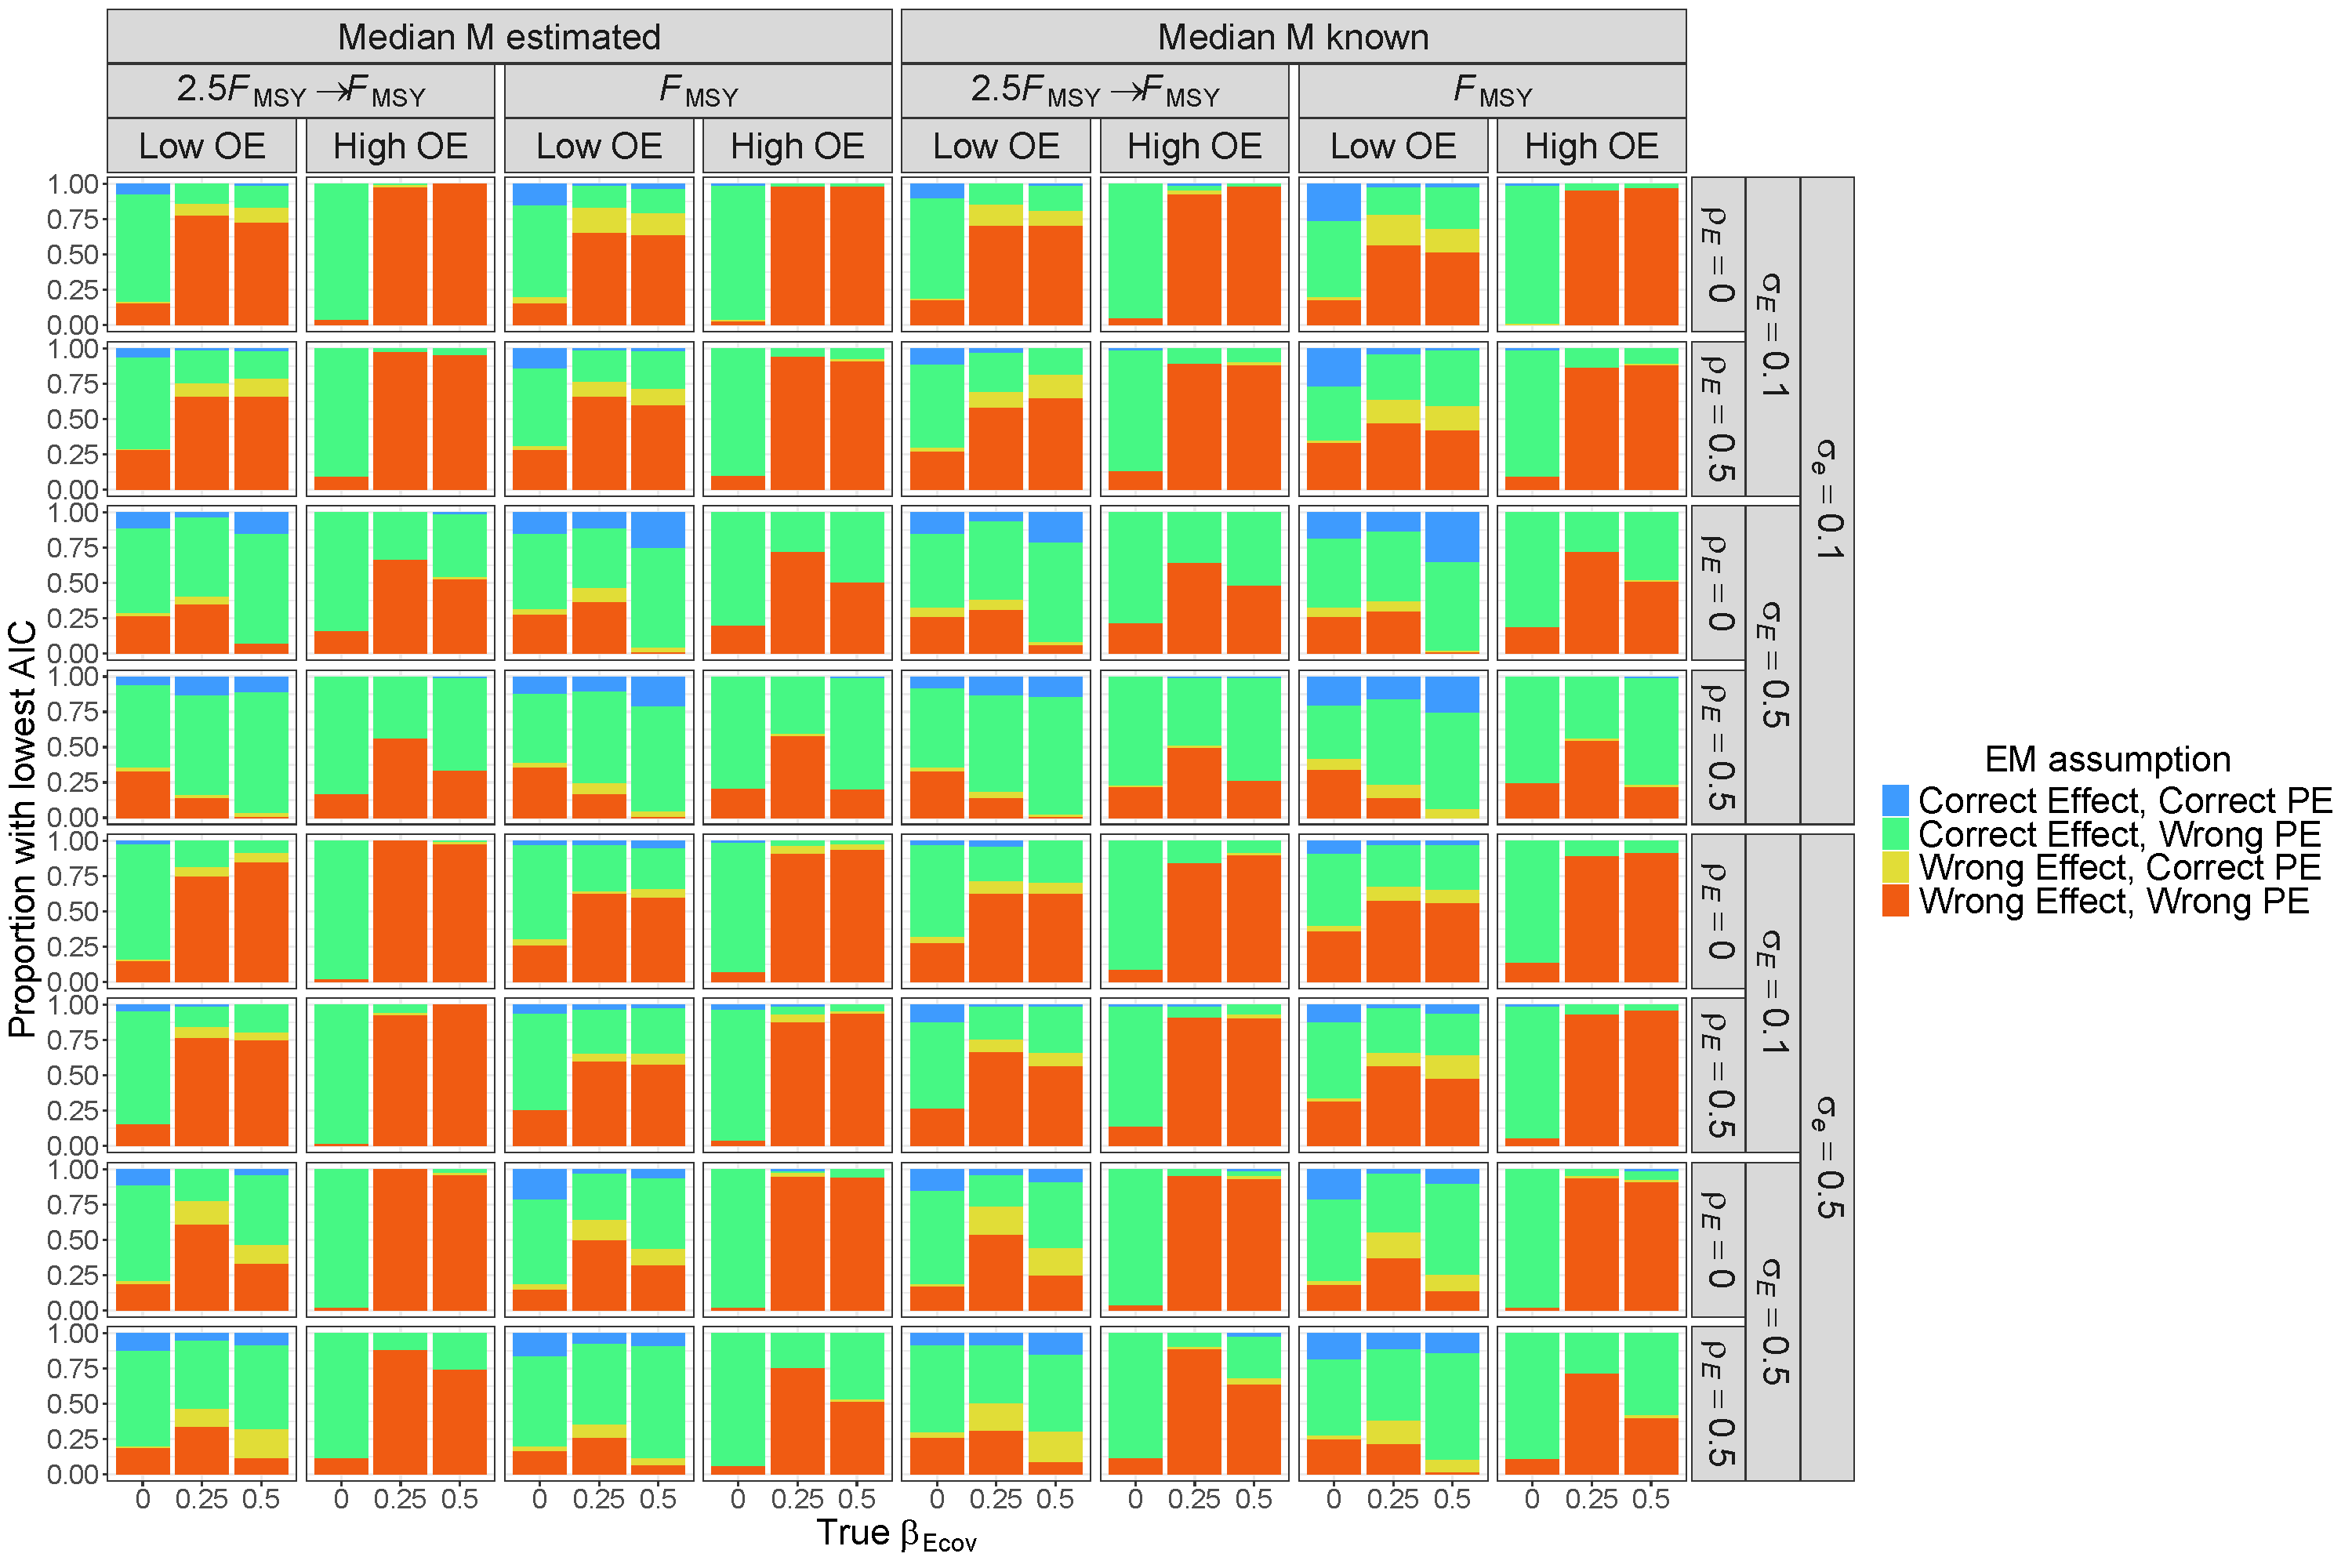
\includegraphics[height = \textheight]{aic_RMom}
\end{center}
\caption{Proportion of simulated data sets for R+M OMs where the EM type (treatment of environmental covariate and assumed process error type) had the lowest AIC.}\label{aic_RMom}
\end{figure}
\end{landscape}

\hypertarget{covariate-effect-bias}{%
\subsection*{Covariate effect bias}\label{covariate-effect-bias}}
\addcontentsline{toc}{subsection}{Covariate effect bias}

\begin{landscape}
\begin{figure}
\begin{center}
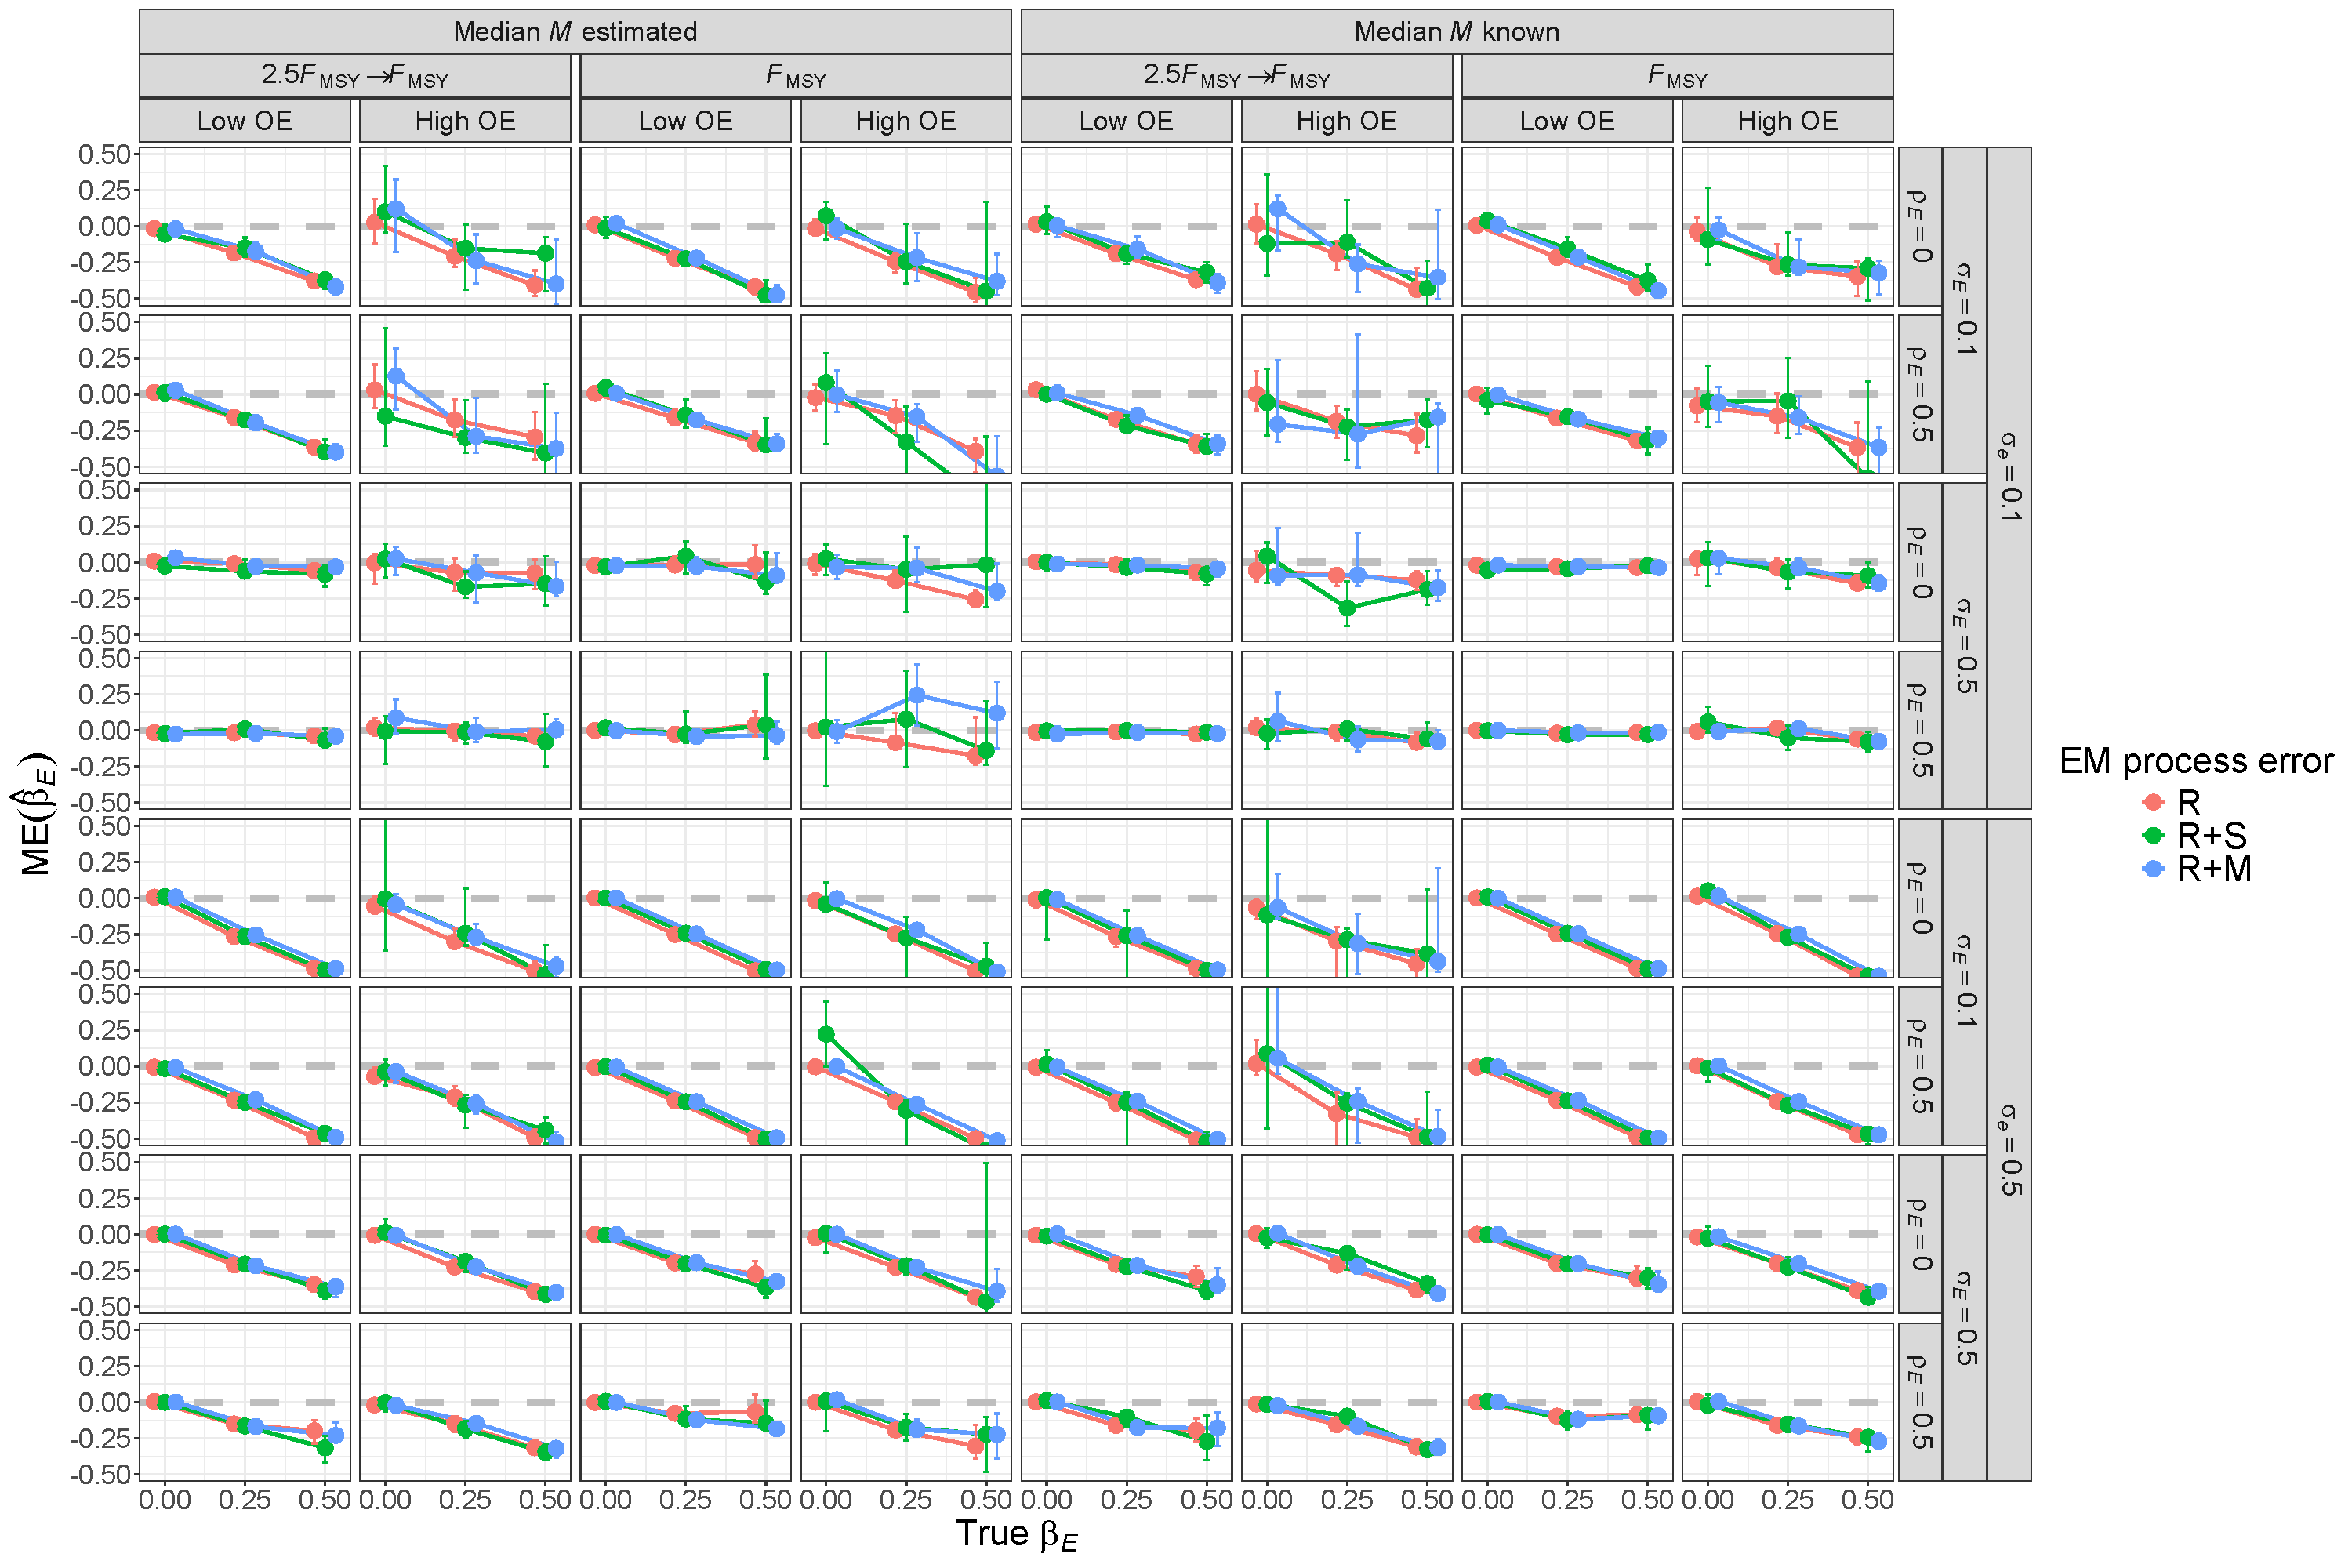
\includegraphics[height = \textheight]{beta_E_bias_Rom}
\end{center}
\caption{For R OMs, median error (ME) of estimates of environmental effect on natural mortality $\beta_E$ from fitting EMs with alternative process error assumptions and treatment of median natural mortality ($e^\beta_M$ known or estimated). Vertical lines represent 95\% confidence intervals.}\label{beta_E_bias_Rom}
\end{figure}
\end{landscape}

\begin{landscape}
\begin{figure}
\begin{center}
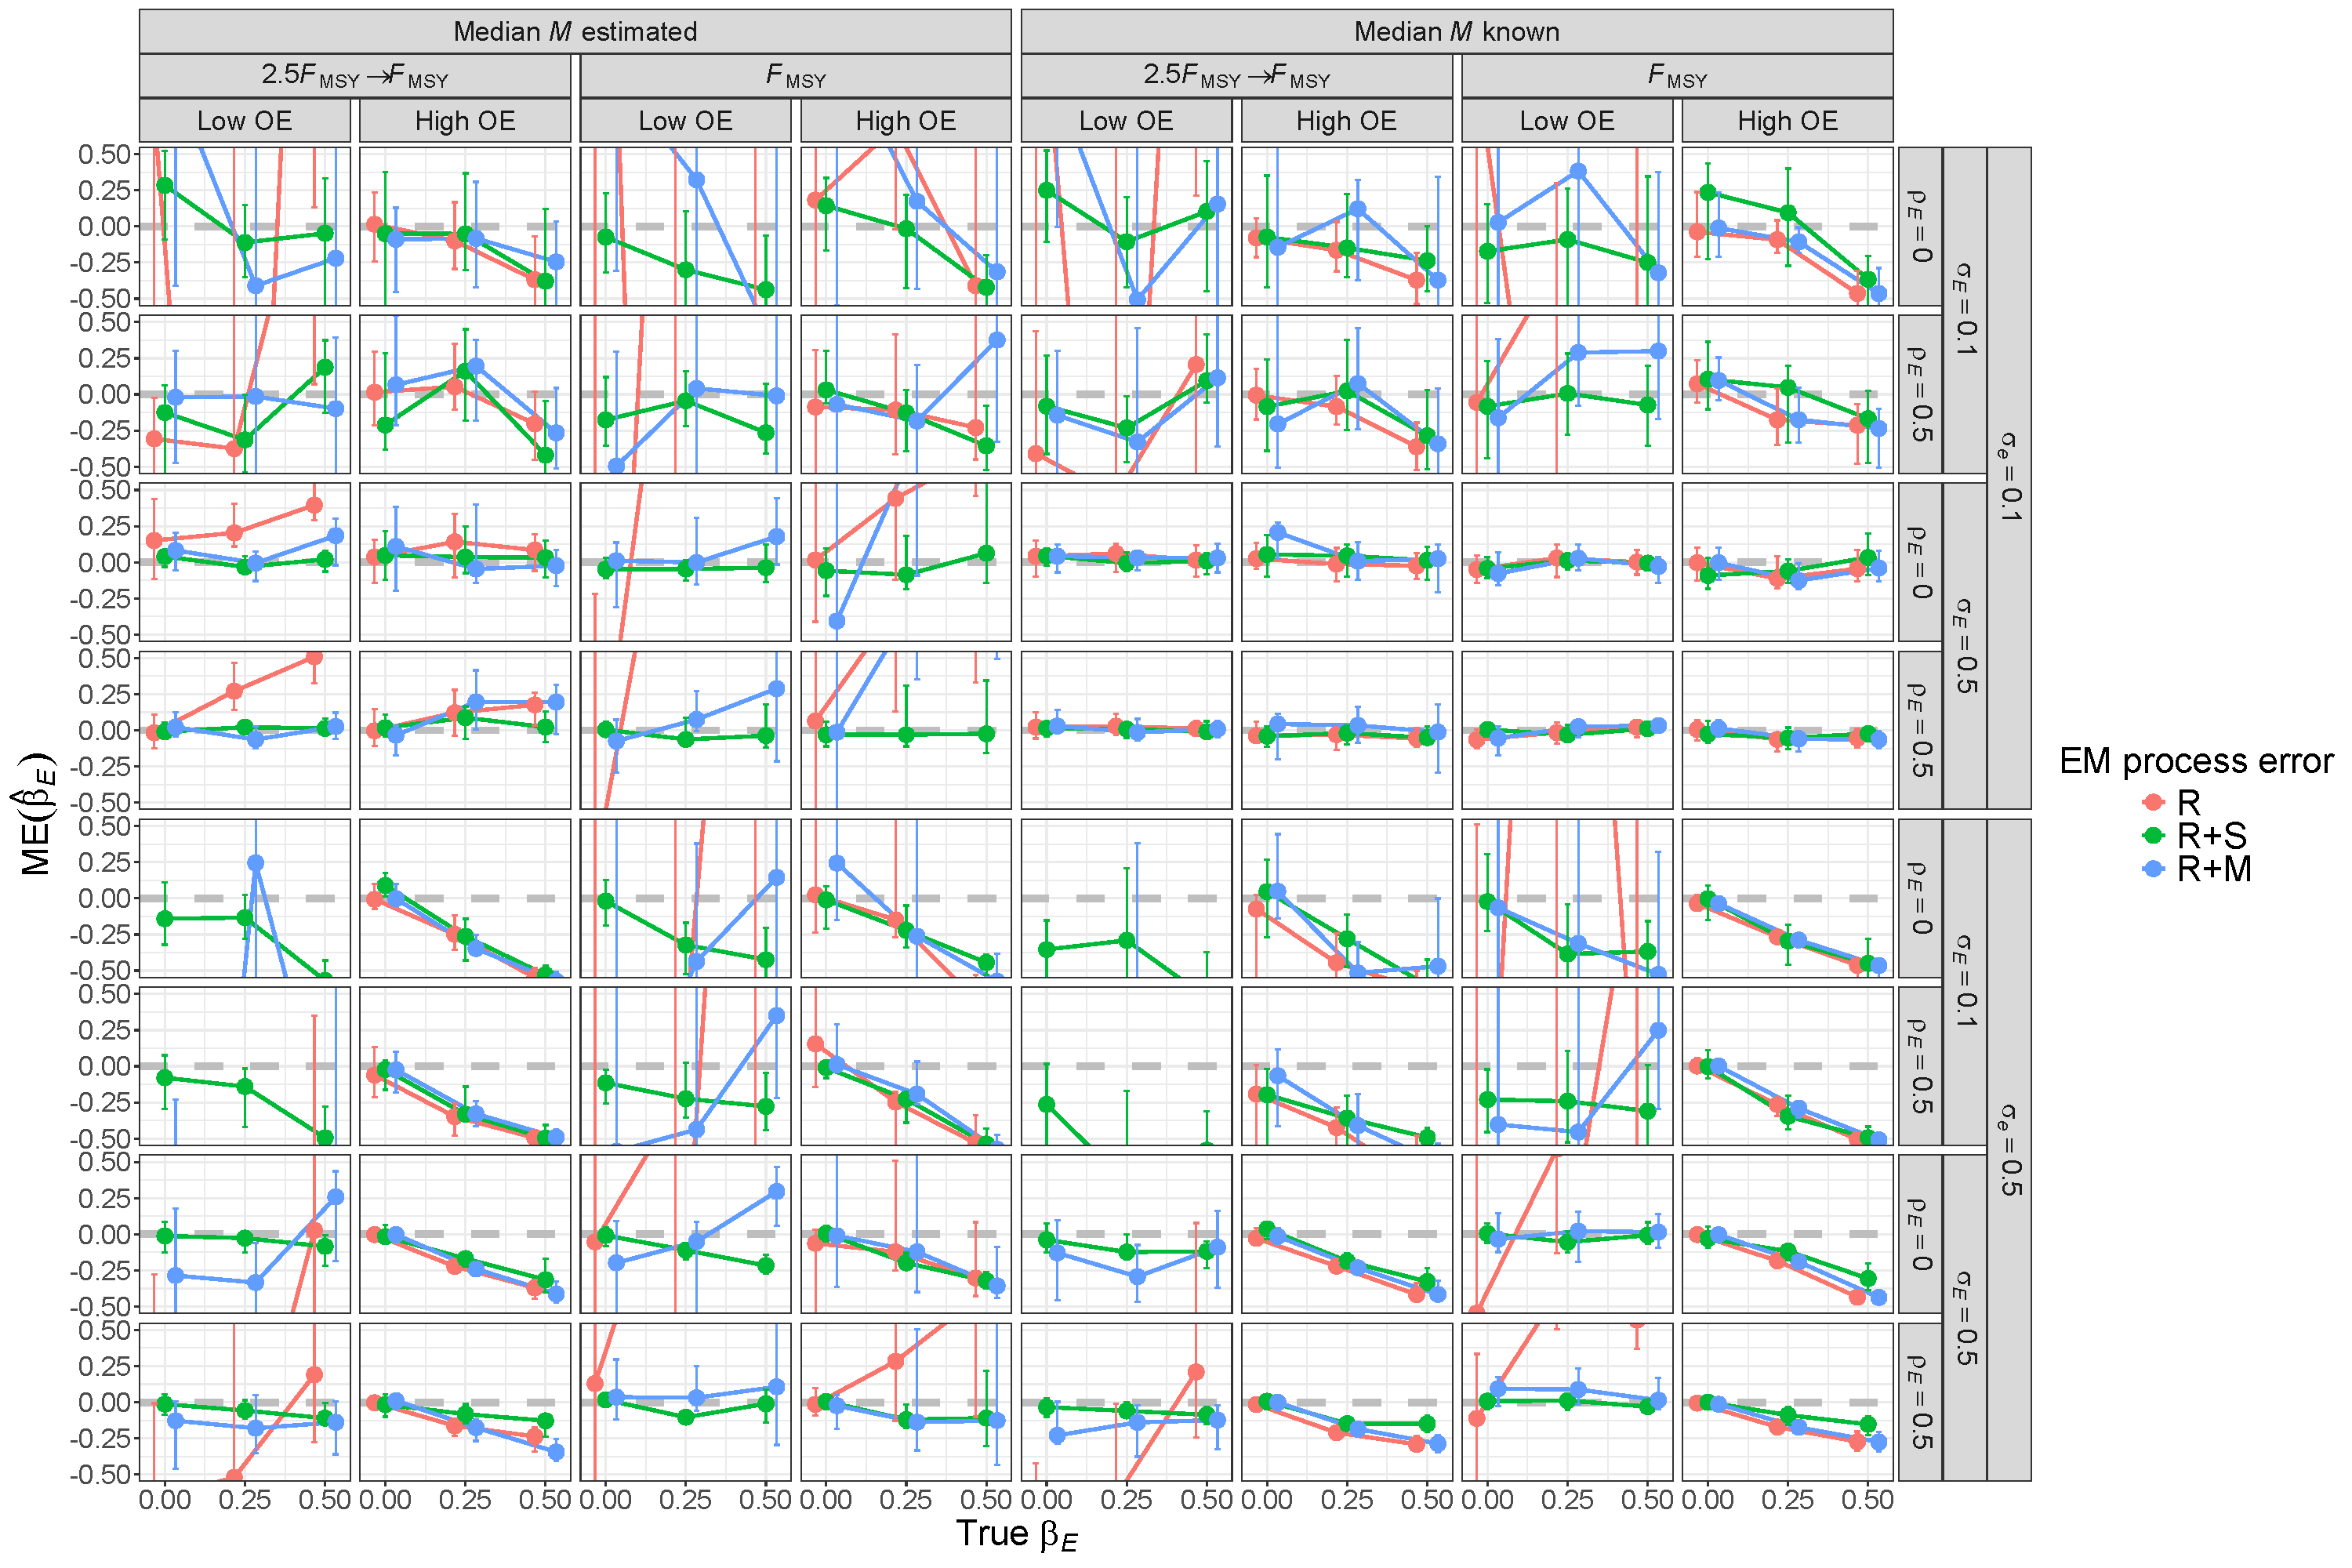
\includegraphics[height = \textheight]{beta_E_bias_RSom}
\end{center}
\caption{For R+S OMs, median error (ME) of estimates of environmental effect on natural mortality $\beta_E$ from fitting EMs with alternative process error assumptions and treatment of median natural mortality ($e^\beta_M$ known or estimated). Vertical lines represent 95\% confidence intervals.}\label{beta_E_bias_RSom}
\end{figure}
\end{landscape}

\begin{landscape}
\begin{figure}
\begin{center}
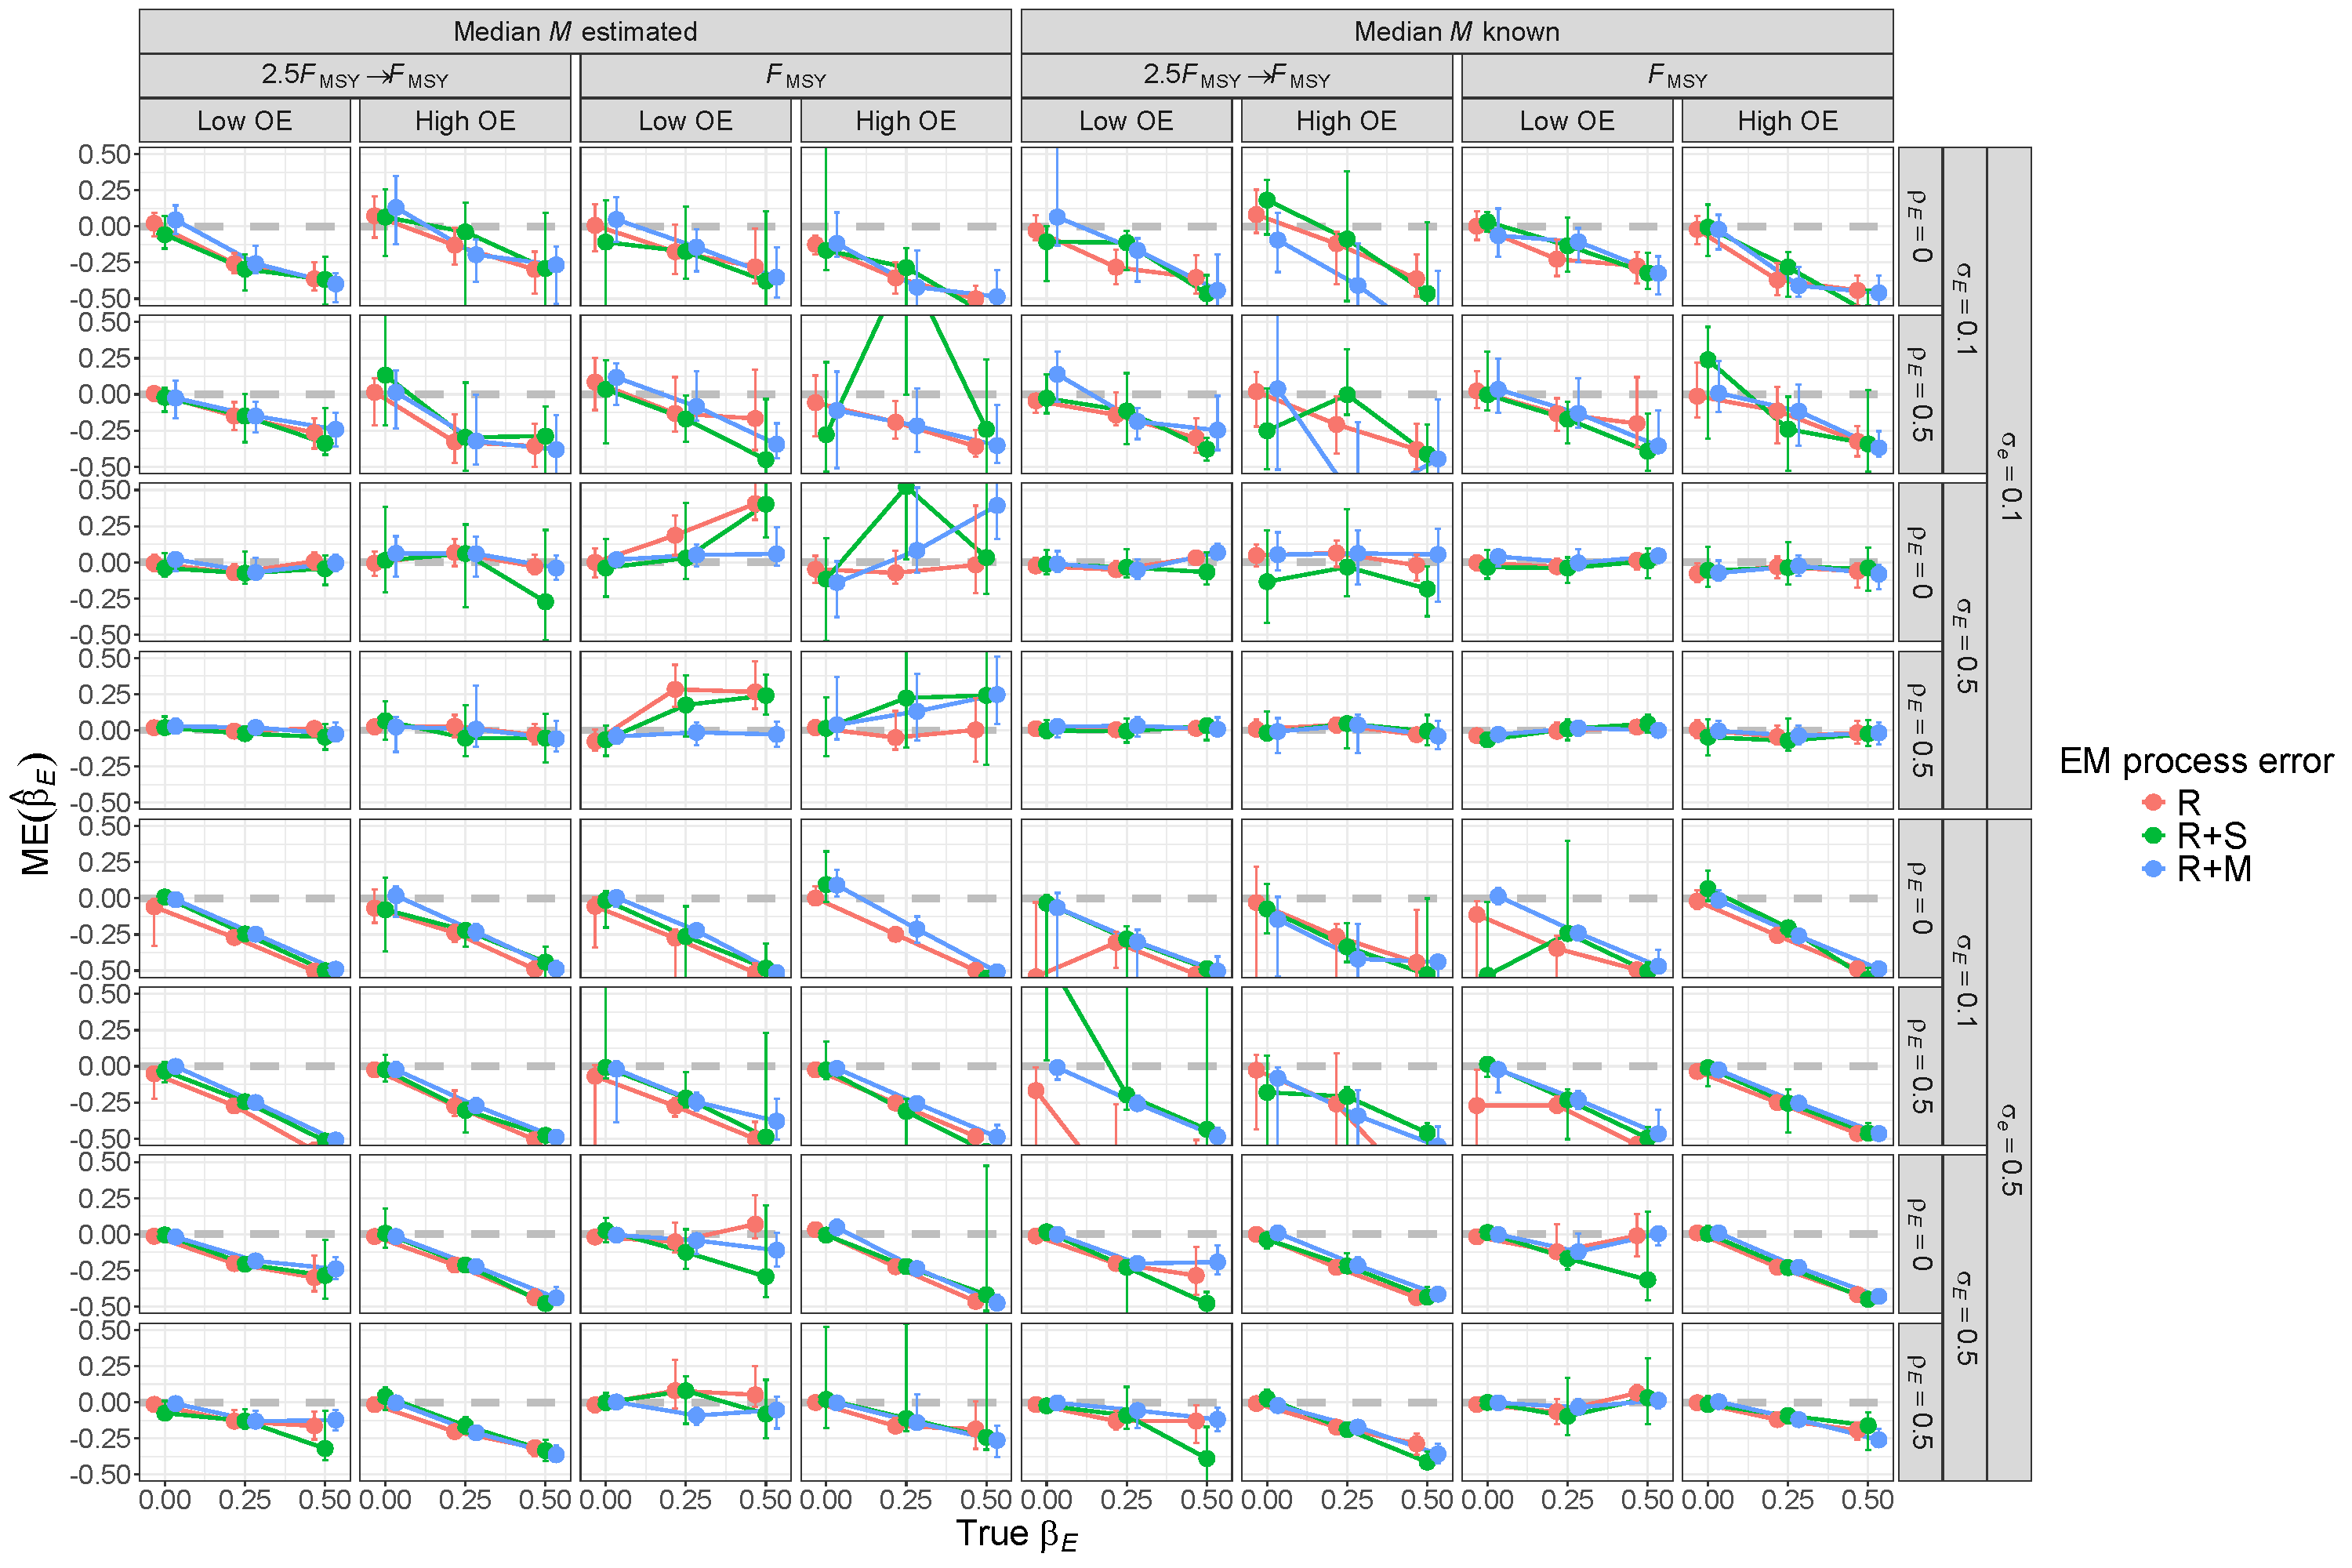
\includegraphics[height = \textheight]{beta_E_bias_RMom}
\end{center}
\caption{For R+M OMs, median error (ME) of estimates of environmental effect on natural mortality $\beta_E$ from fitting EMs with alternative process error assumptions and treatment of median natural mortality ($e^\beta_M$ known or estimated). Vertical lines represent 95\% confidence intervals.}\label{beta_E_bias_RMom}
\end{figure}
\end{landscape}

\hypertarget{covariate-effect-standard-error-estimation-bias}{%
\subsection*{Covariate effect standard error estimation bias}\label{covariate-effect-standard-error-estimation-bias}}
\addcontentsline{toc}{subsection}{Covariate effect standard error estimation bias}

\begin{landscape}
\begin{figure}
\begin{center}
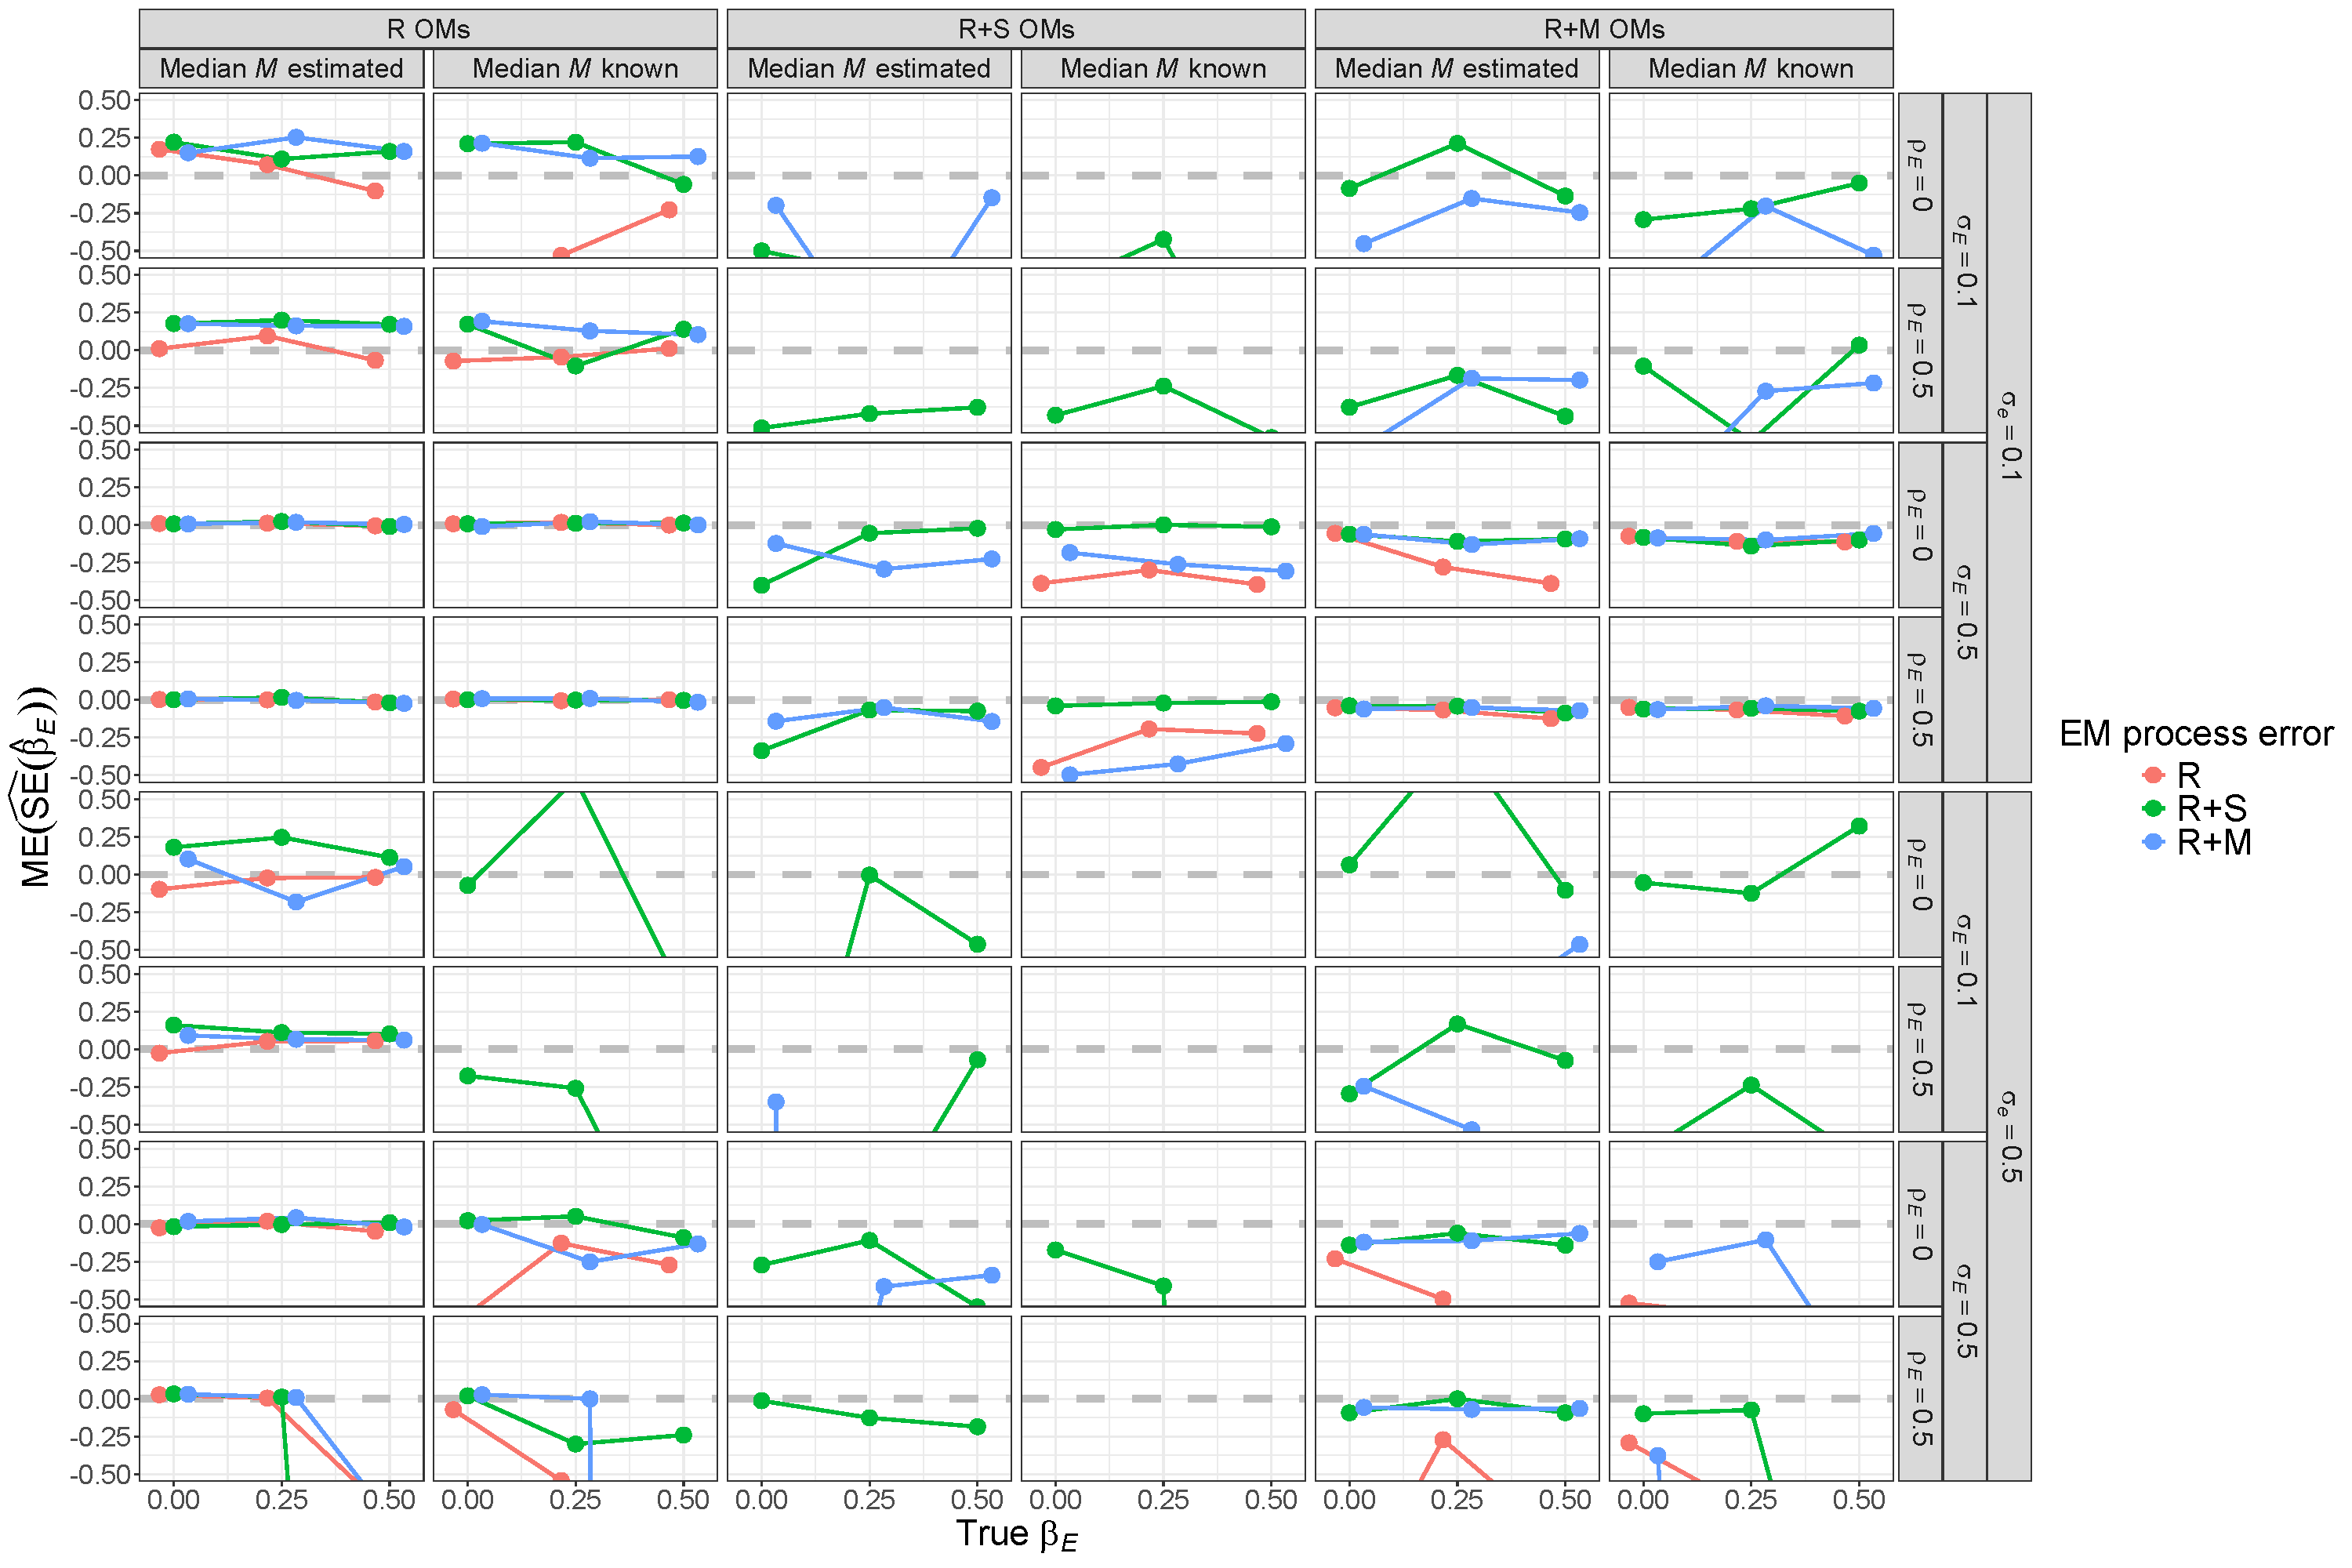
\includegraphics[height = \textheight]{se_beta_E_bias_main}
\end{center}
\caption{Median error (ME) of Hessian-based estimates of standard error for covariate effect on natural mortality $\beta_E$ from fitting EMs with alternative process error assumptions and treatment of median natural mortality ($e^\beta_M$ known or estimated). All OMs had low observation error and contrast in fishing mortality. True standard error is defined as the mean of the standard error estimates accross converged fits to simulated data sets for a given OM scenario.}\label{se_beta_E_bias}
\end{figure}
\end{landscape}

\begin{landscape}
\begin{figure}
\begin{center}
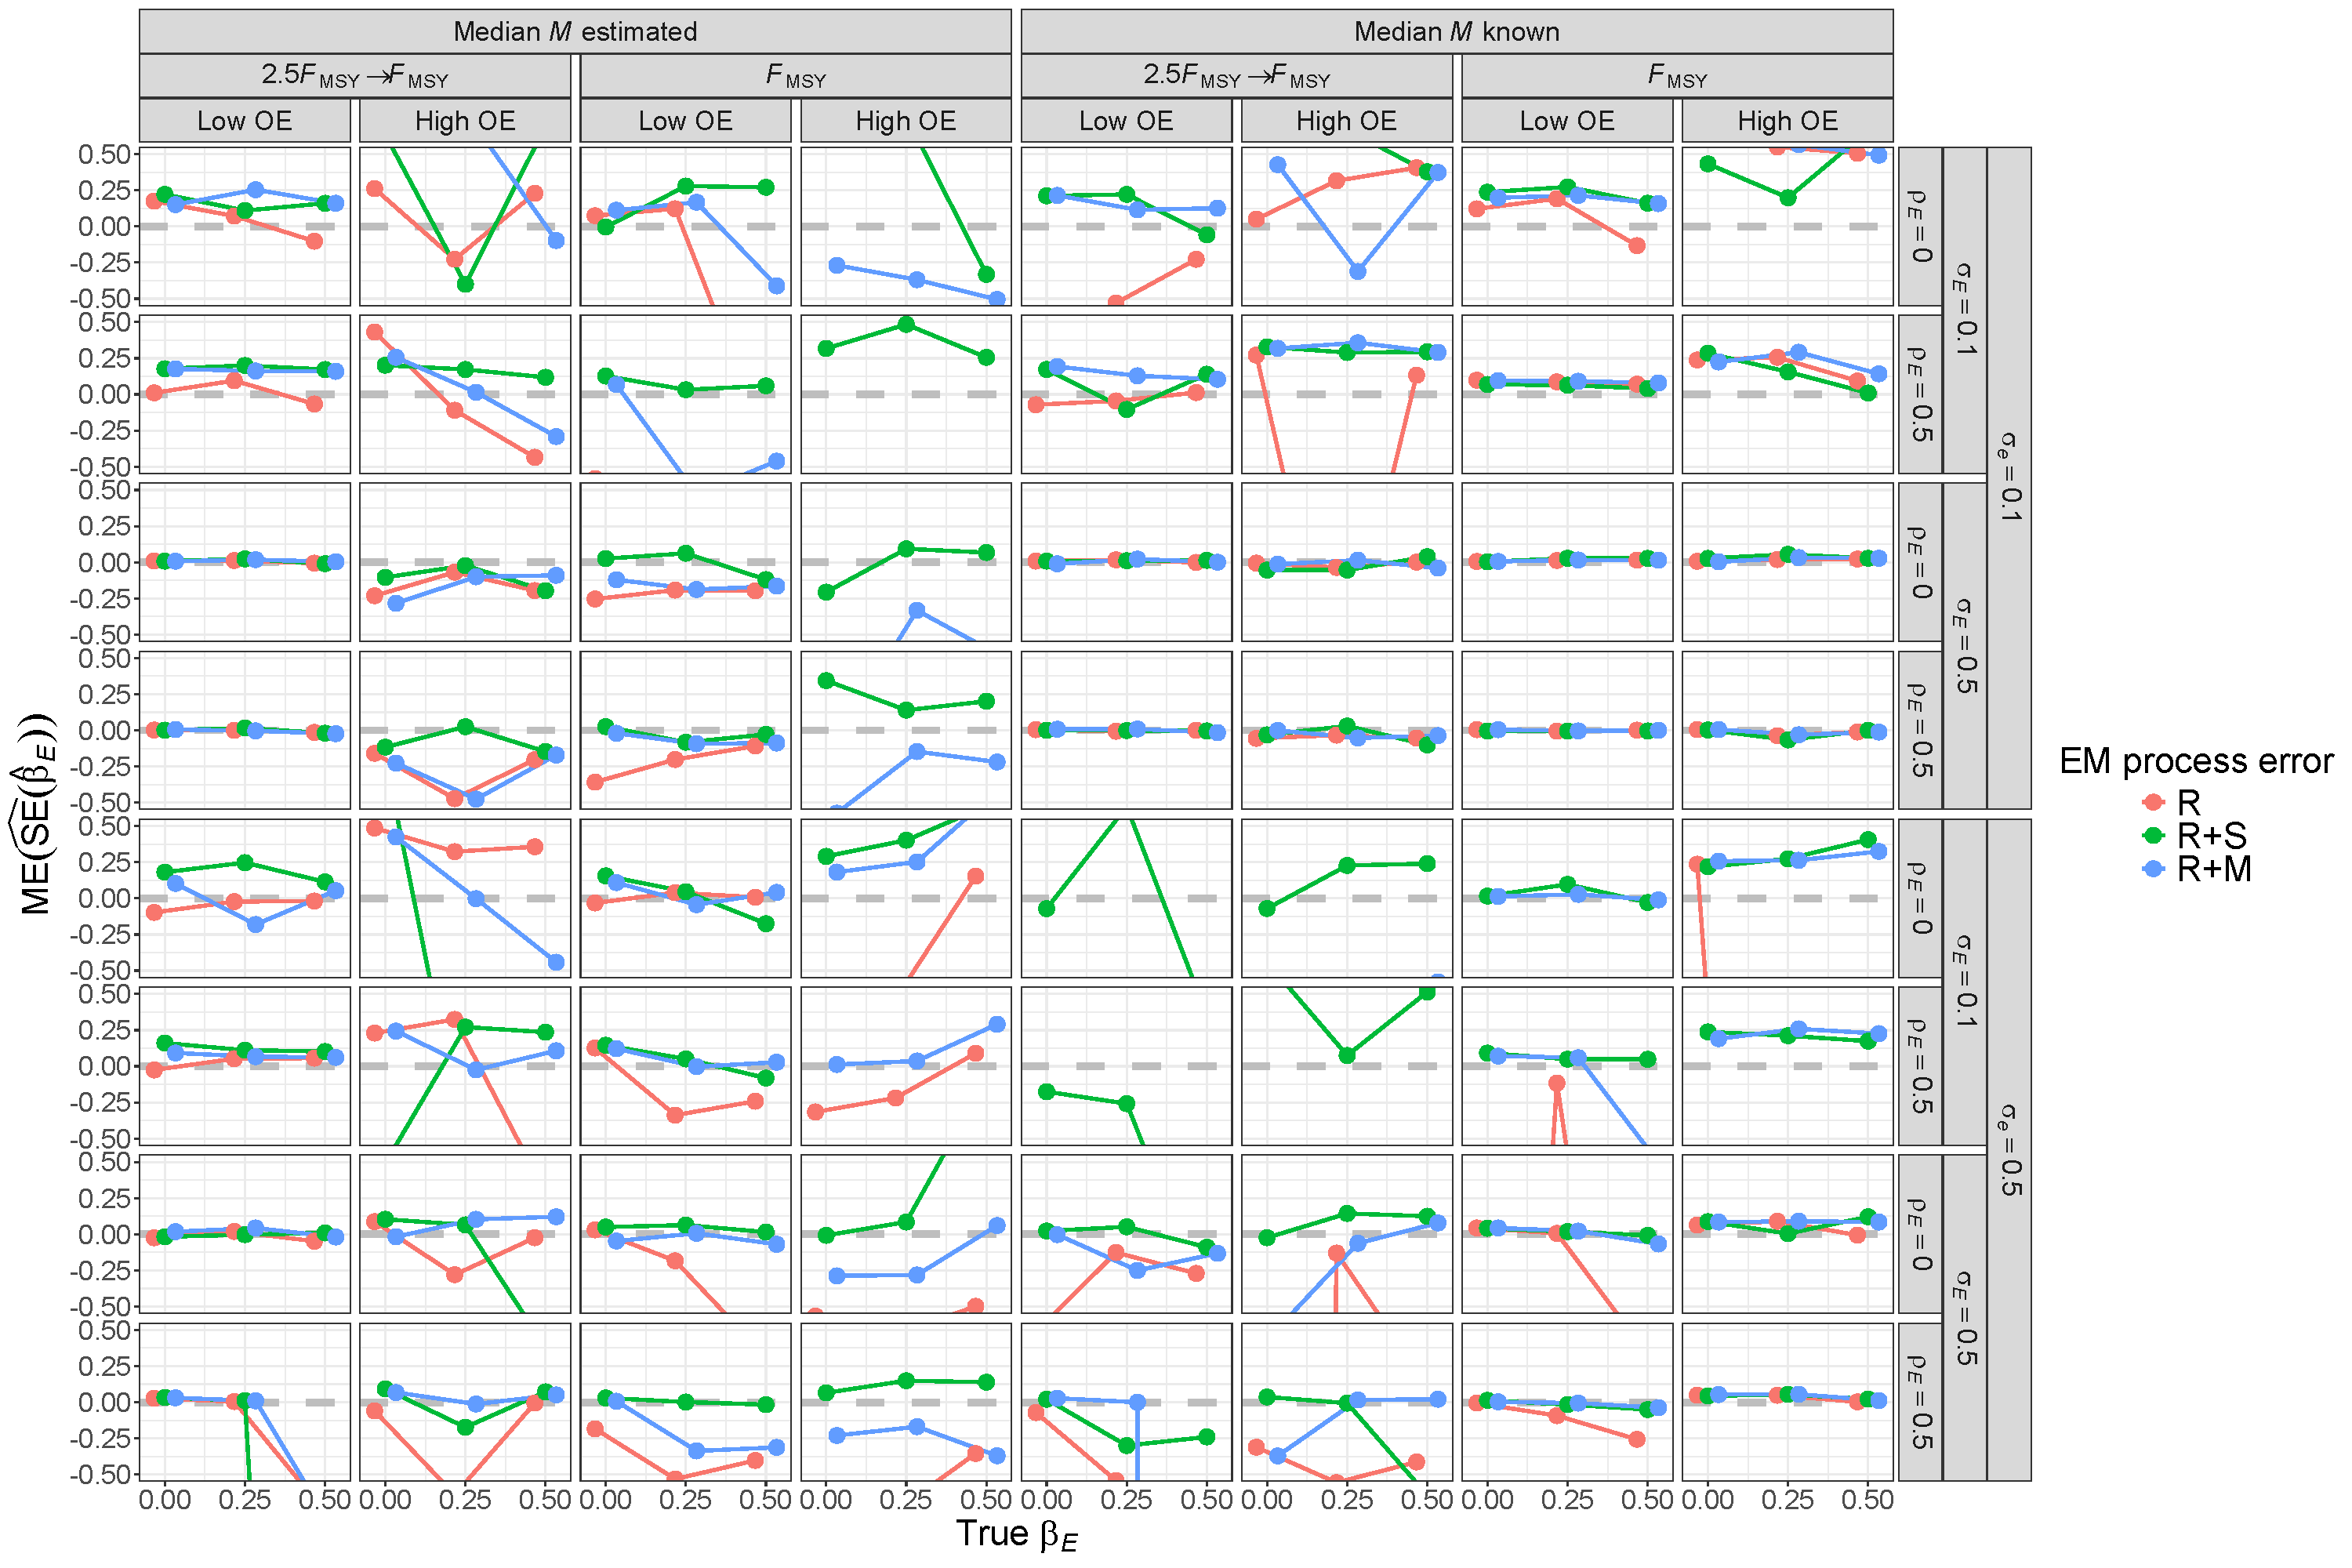
\includegraphics[height = \textheight]{se_beta_E_bias_Rom}
\end{center}
\caption{For R OMs, median error (ME) of Hessian-based estimates of standard error for covariate effect on natural mortality $\beta_E$ from fitting EMs with alternative process error assumptions and treatment of median natural mortality ($e^\beta_M$ known or estimated). True standard error is defined as the mean of the standard error estimates accross converged fits to simulated data sets for a given OM scenario.}\label{se_beta_E_bias_Rom}
\end{figure}
\end{landscape}

\begin{landscape}
\begin{figure}
\begin{center}
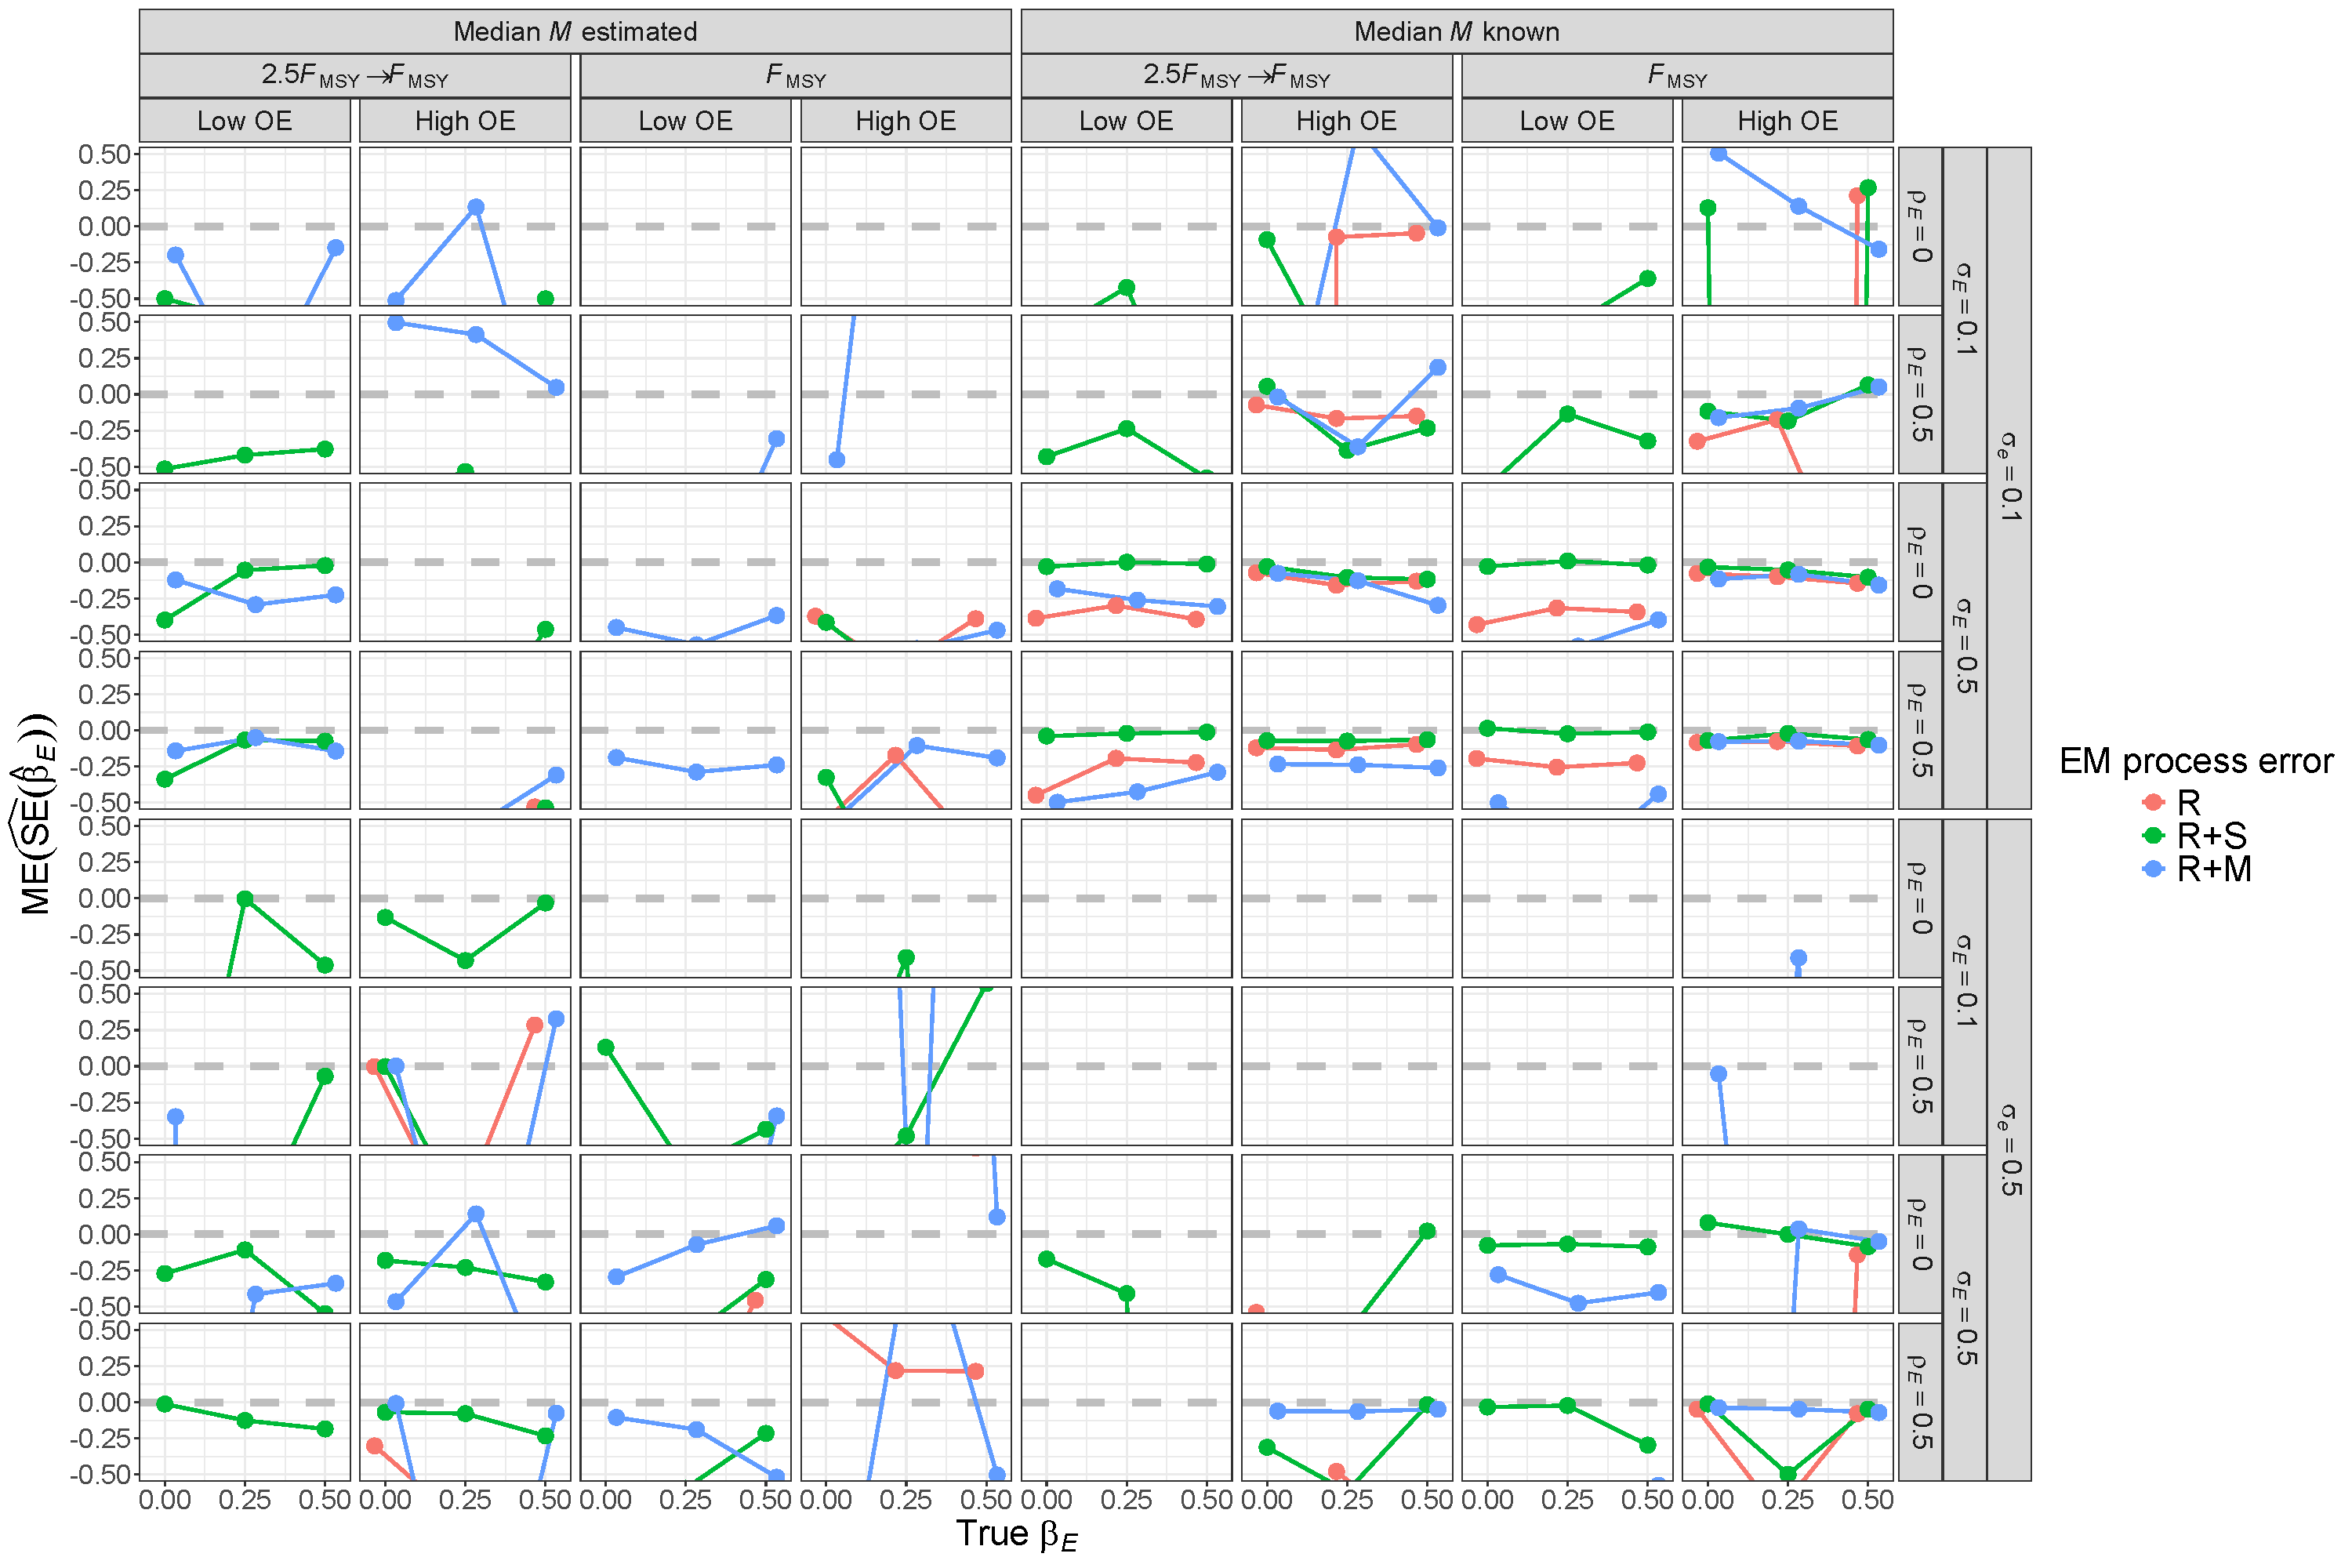
\includegraphics[height = \textheight]{se_beta_E_bias_RSom}
\end{center}
\caption{For R+S OMs, median error (ME) of Hessian-based estimates of standard error for covariate effect on natural mortality $\beta_E$ from fitting EMs with alternative process error assumptions and treatment of median natural mortality ($e^\beta_M$ known or estimated). True standard error is defined as the mean of the standard error estimates accross converged fits to simulated data sets for a given OM scenario.}\label{se_beta_E_bias_RSom}
\end{figure}
\end{landscape}

\begin{landscape}
\begin{figure}
\begin{center}
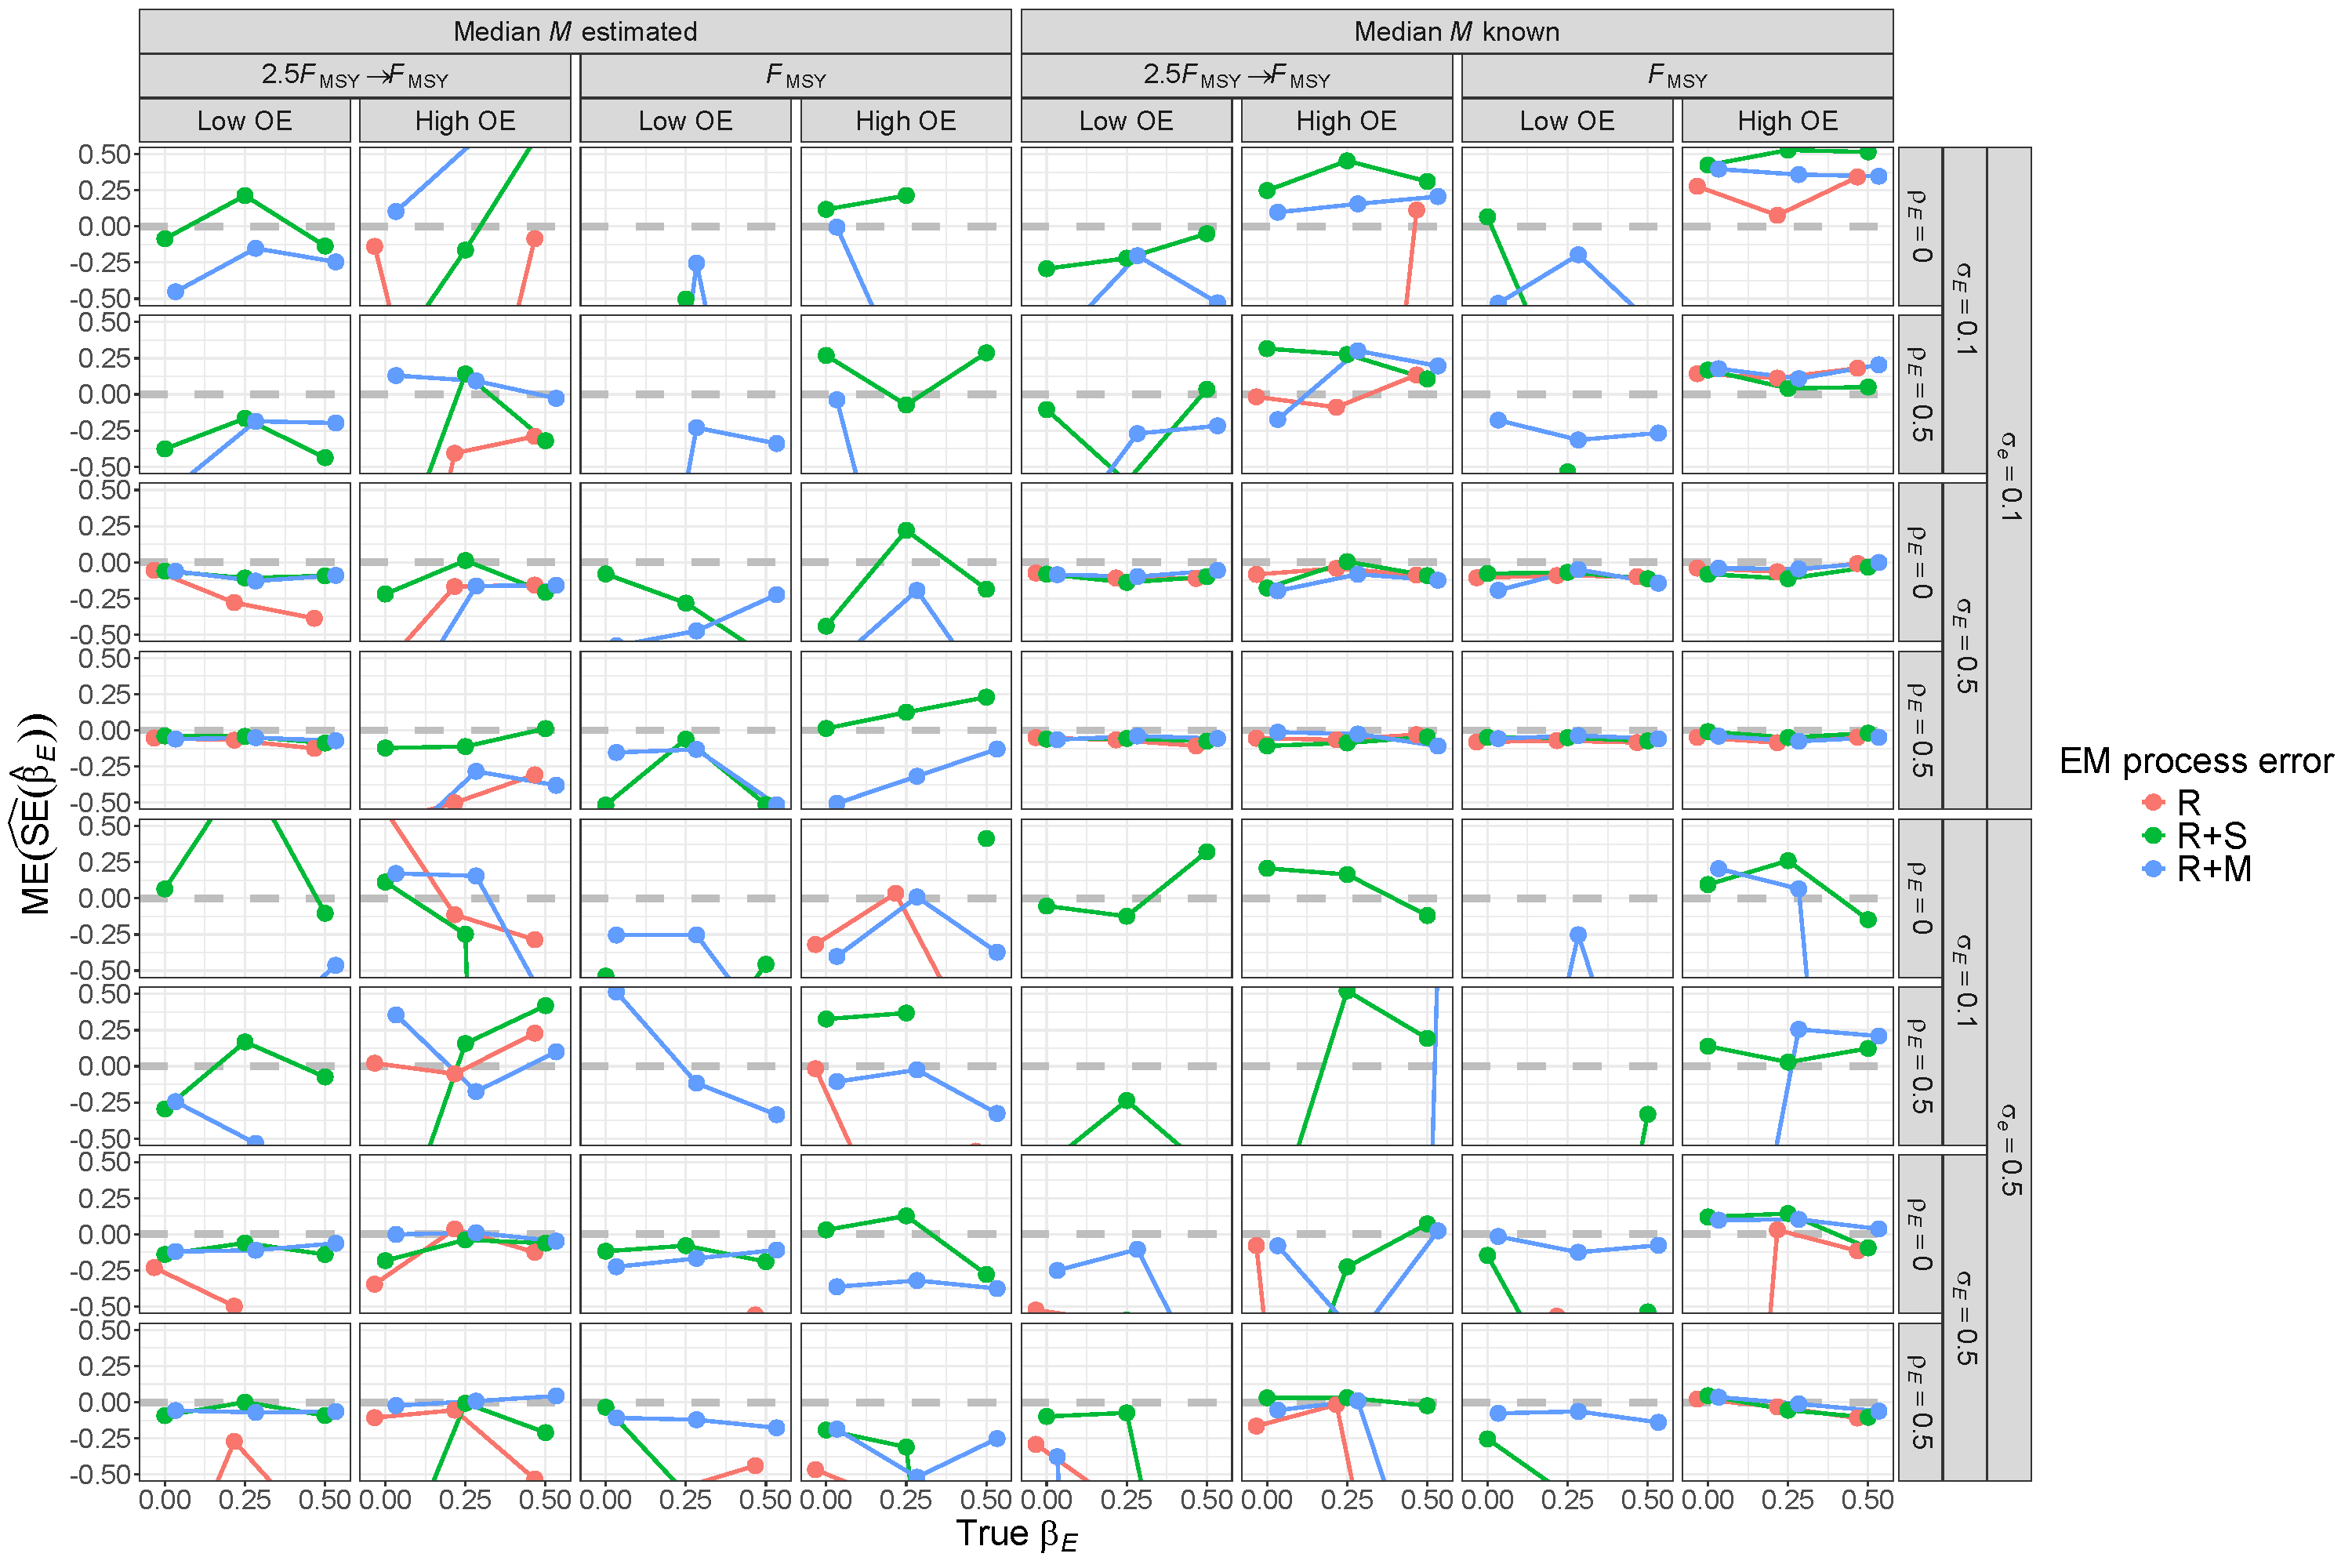
\includegraphics[height = \textheight]{se_beta_E_bias_RMom}
\end{center}
\caption{For R+M OMs, median error (ME) of Hessian-based estimates of standard error for covariate effect on natural mortality $\beta_E$ from fitting EMs with alternative process error assumptions and treatment of median natural mortality ($e^\beta_M$ known or estimated). True standard error is defined as the mean of the standard error estimates accross converged fits to simulated data sets for a given OM scenario.}\label{se_beta_E_bias_RMom}
\end{figure}
\end{landscape}

\hypertarget{covariate-effect-confidence-interval-coverage}{%
\subsection*{Covariate effect confidence interval coverage}\label{covariate-effect-confidence-interval-coverage}}
\addcontentsline{toc}{subsection}{Covariate effect confidence interval coverage}

\begin{landscape}
\begin{figure}
\begin{center}
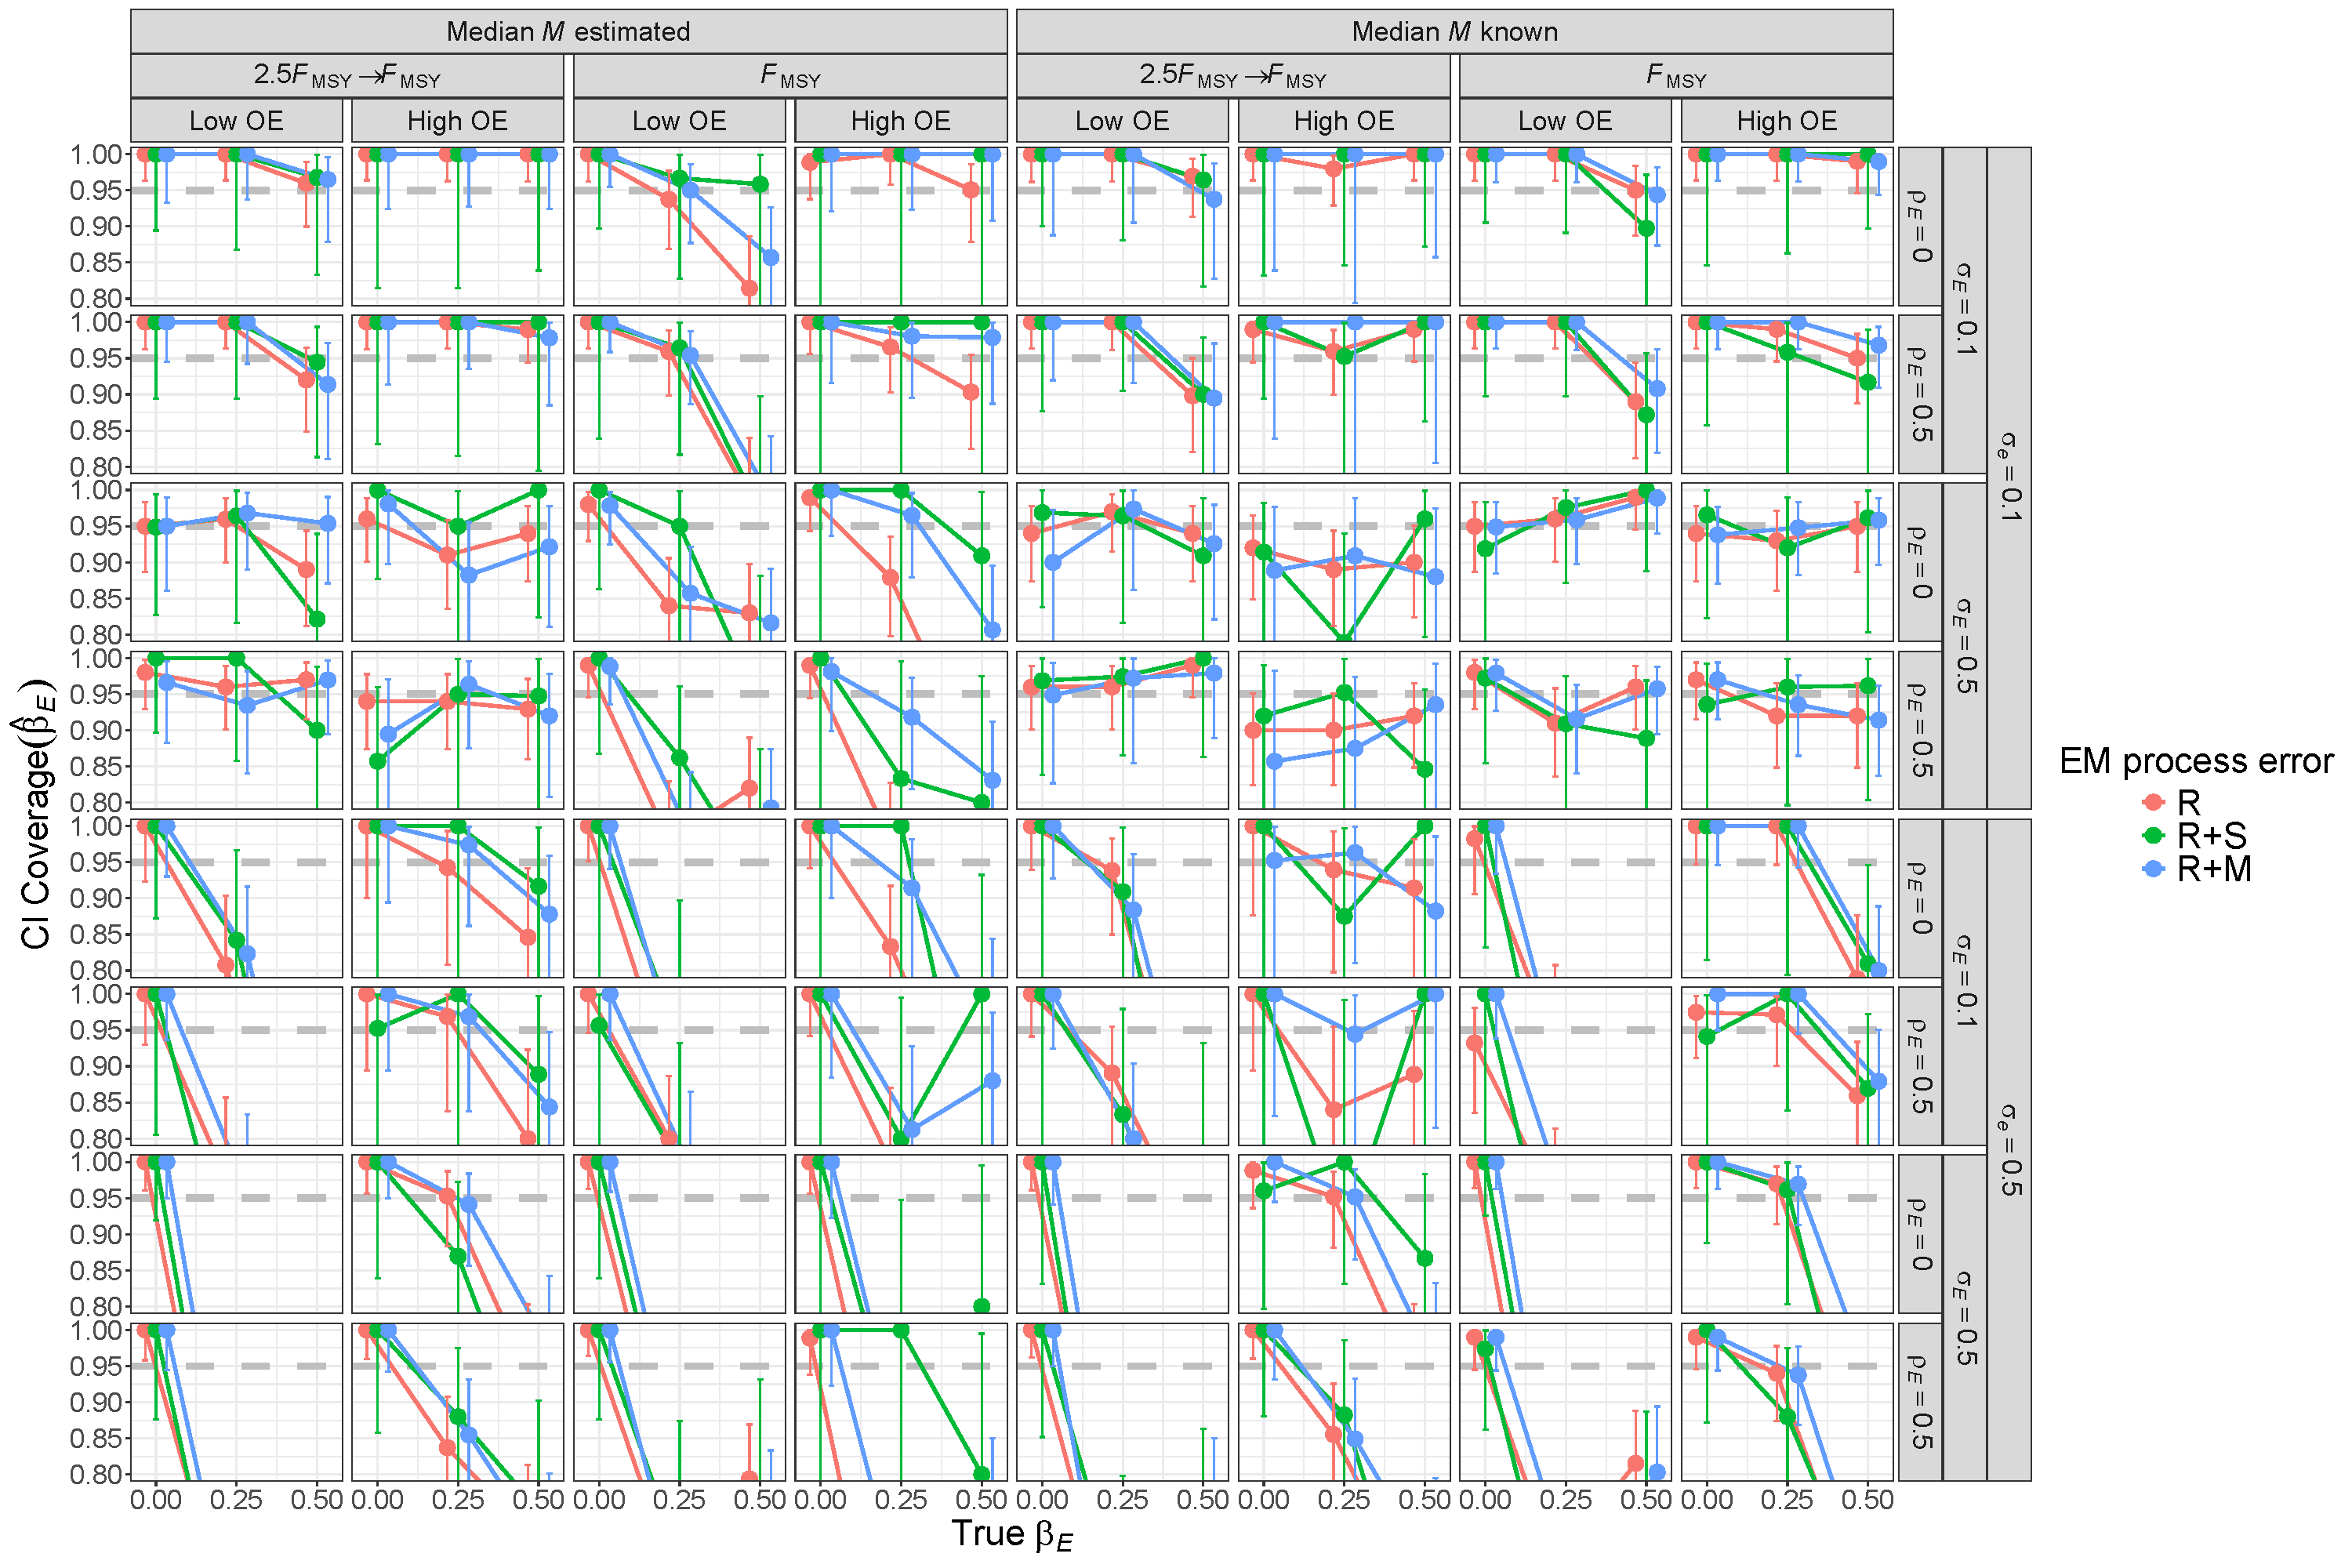
\includegraphics[height = \textheight]{beta_E_CI_coverage_Rom}
\end{center}
\caption{For R OMs, probability of 95\% confidence interval for $\beta_E$ containing the true value for EMs with alternative process error assumptions and treatment of median natural mortality ($e^\beta_M$ known or estimated). Vertical lines represent 95\% confidence intervals.}\label{beta_E_CI_coverage_Rom}
\end{figure}
\end{landscape}

\begin{landscape}
\begin{figure}
\begin{center}
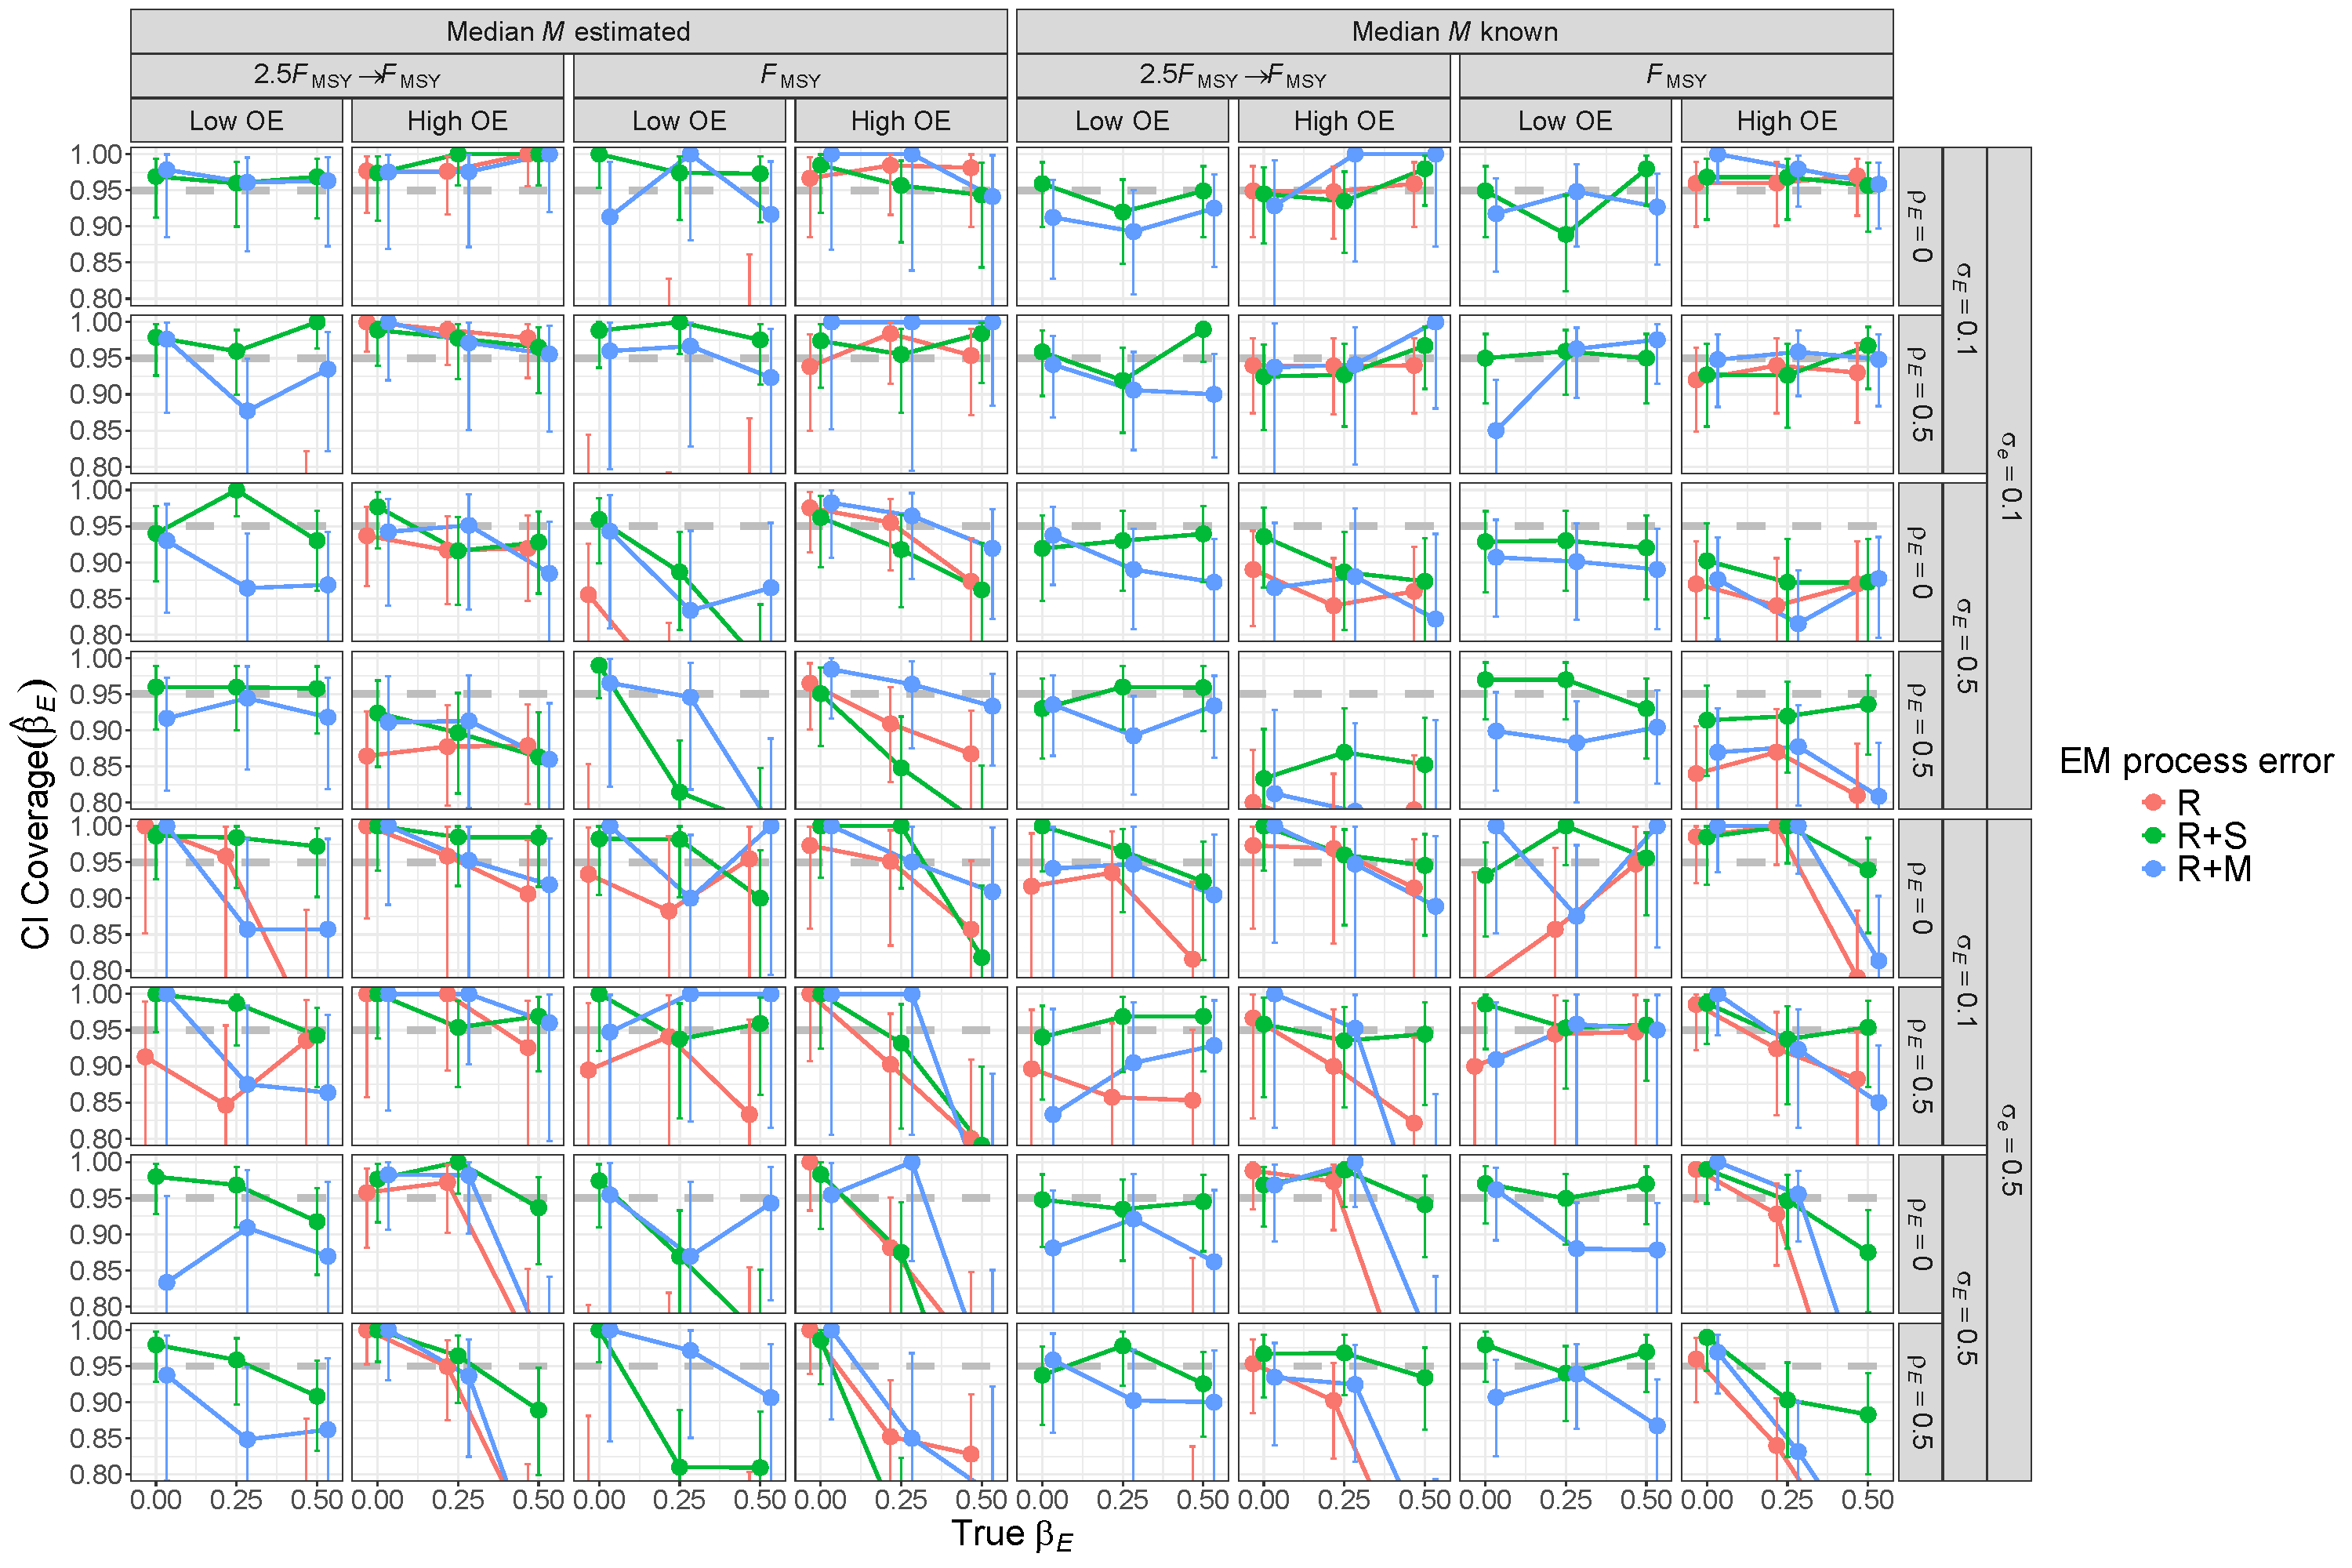
\includegraphics[height = \textheight]{beta_E_CI_coverage_RSom}
\end{center}
\caption{For R+S OMs, probability of 95\% confidence interval for $\beta_E$ containing the true value for EMs with alternative process error assumptions and treatment of median natural mortality ($e^\beta_M$ known or estimated). Vertical lines represent 95\% confidence intervals.}\label{beta_E_CI_coverage_RSom}
\end{figure}
\end{landscape}

\begin{landscape}
\begin{figure}
\begin{center}
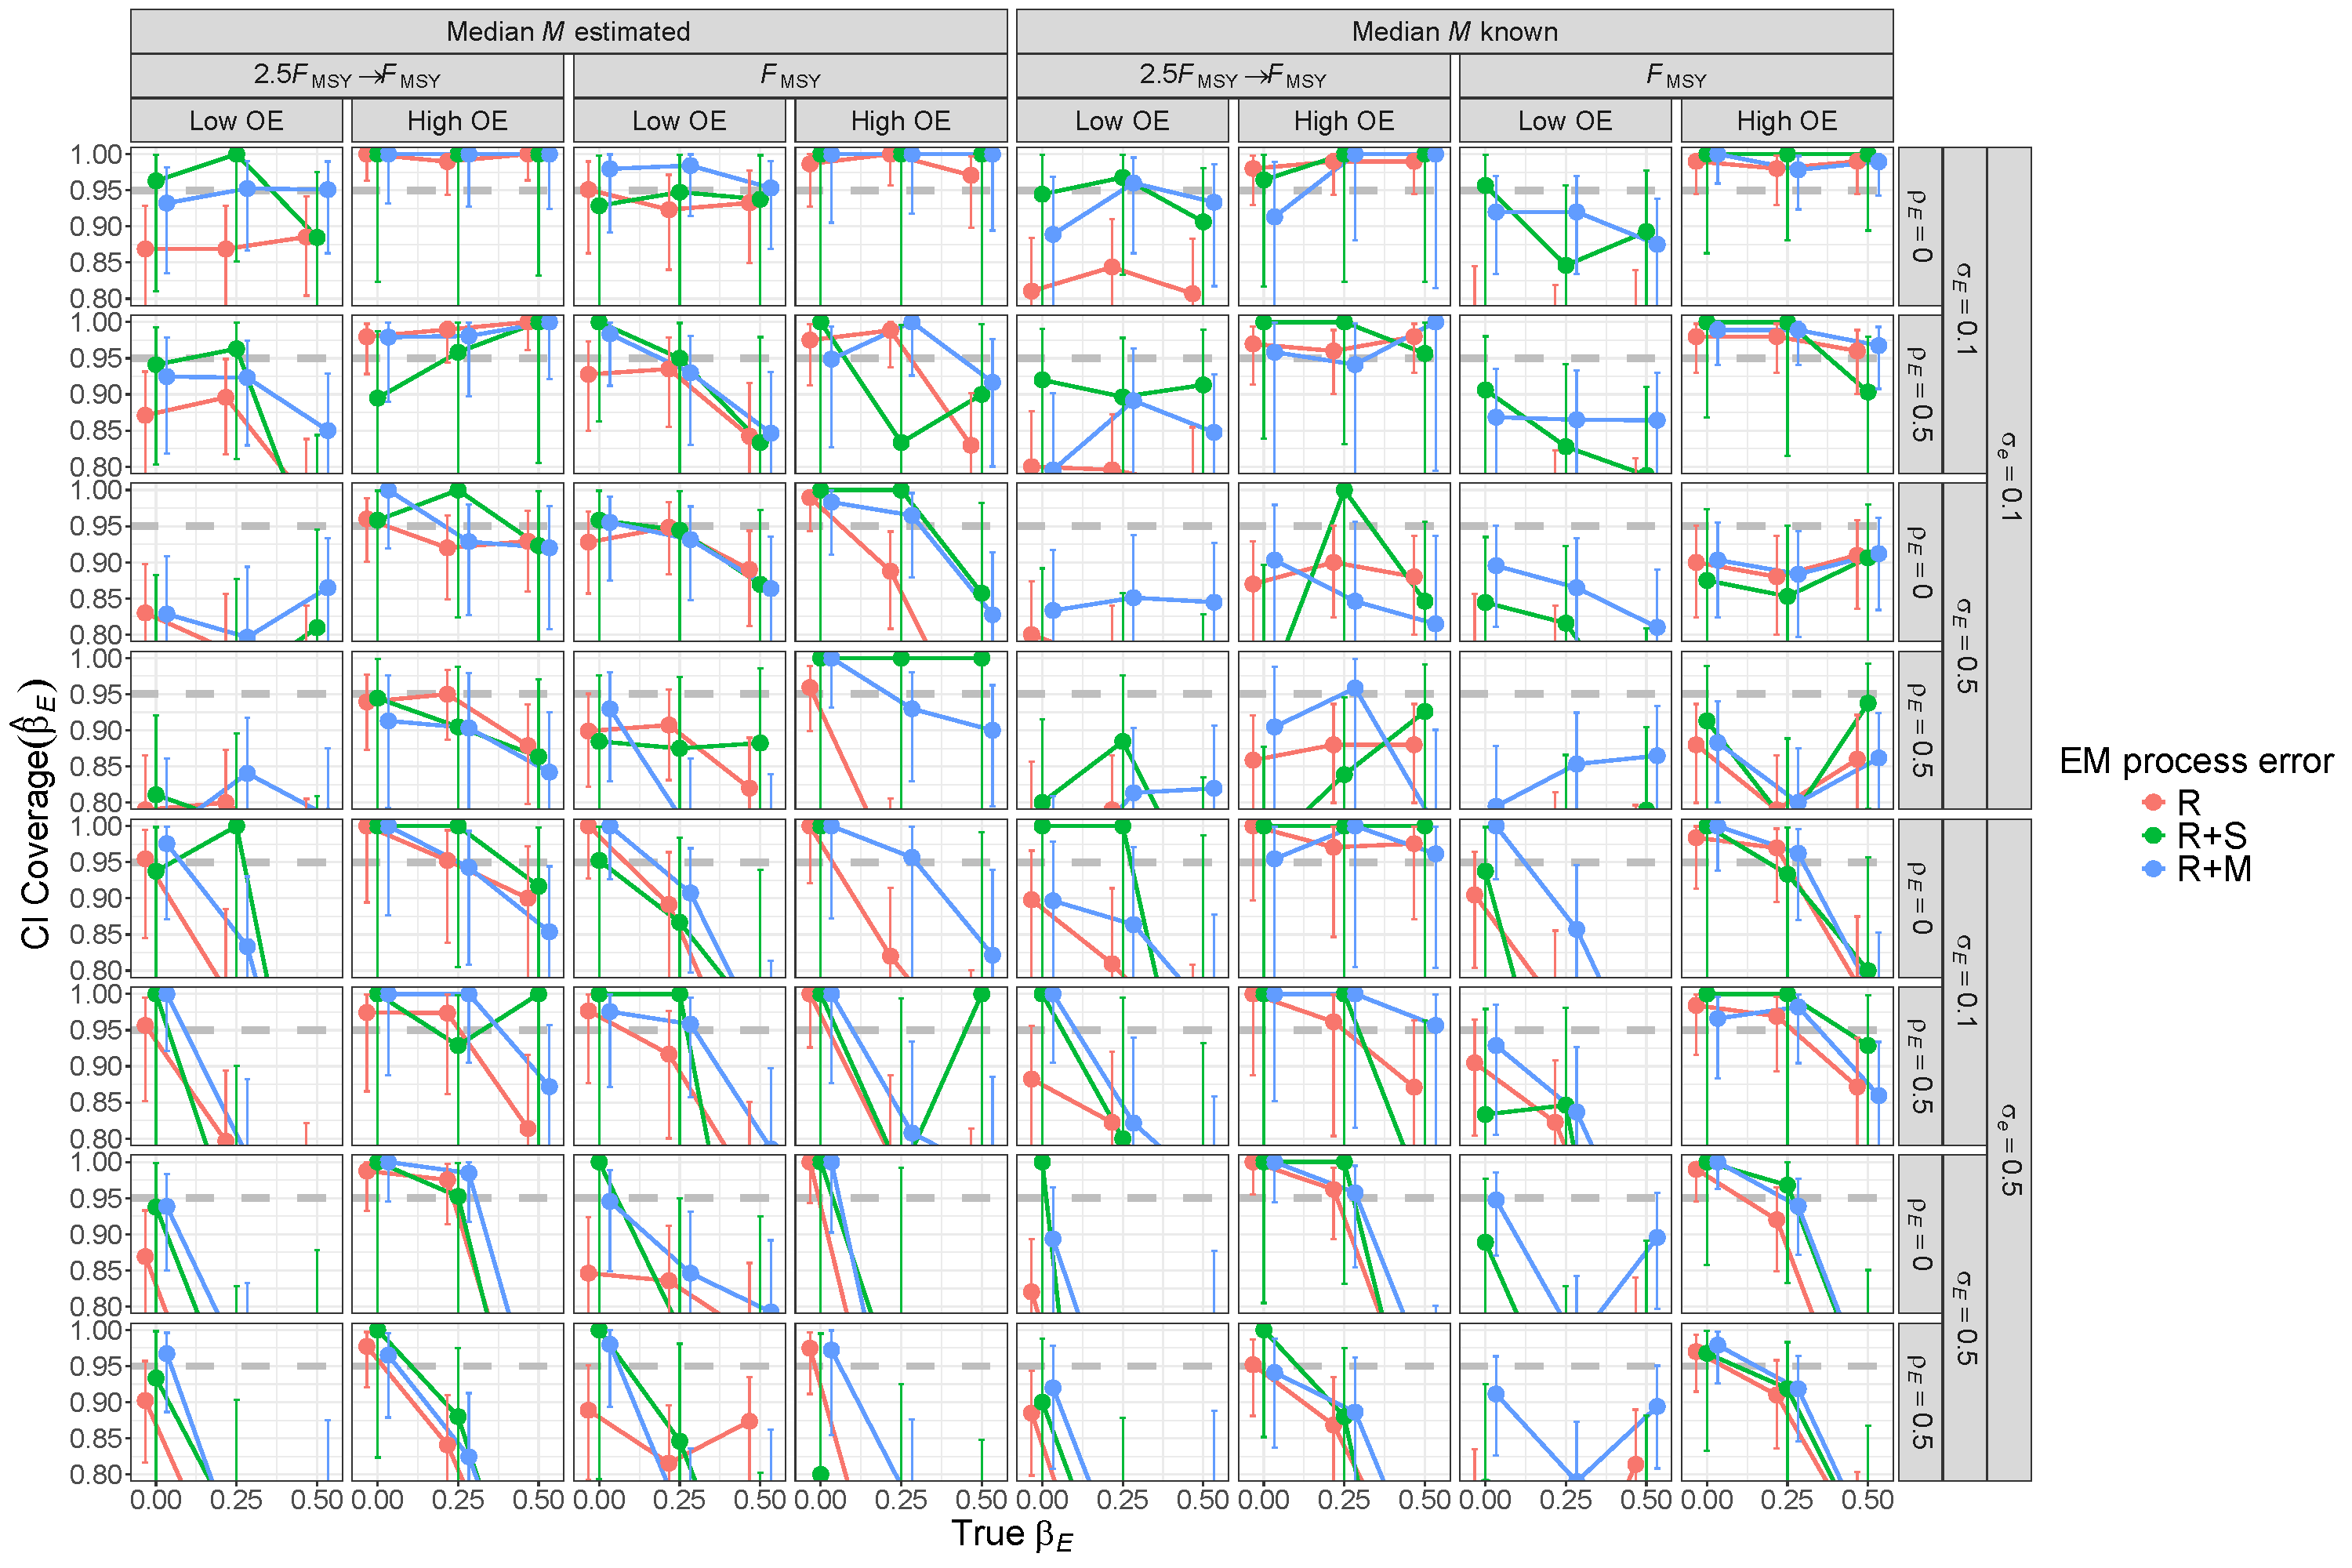
\includegraphics[height = \textheight]{beta_E_CI_coverage_RMom}
\end{center}
\caption{For R+M OMs, probability of 95\% confidence interval for $\beta_E$ containing the true value for EMs with alternative process error assumptions and treatment of median natural mortality ($e^\beta_M$ known or estimated). Vertical lines represent 95\% confidence intervals.}\label{beta_E_CI_coverage_RMom}
\end{figure}
\end{landscape}

\hypertarget{covariate-effect-rmse}{%
\subsection*{Covariate effect RMSE}\label{covariate-effect-rmse}}
\addcontentsline{toc}{subsection}{Covariate effect RMSE}

\begin{landscape}
\begin{figure}
\begin{center}
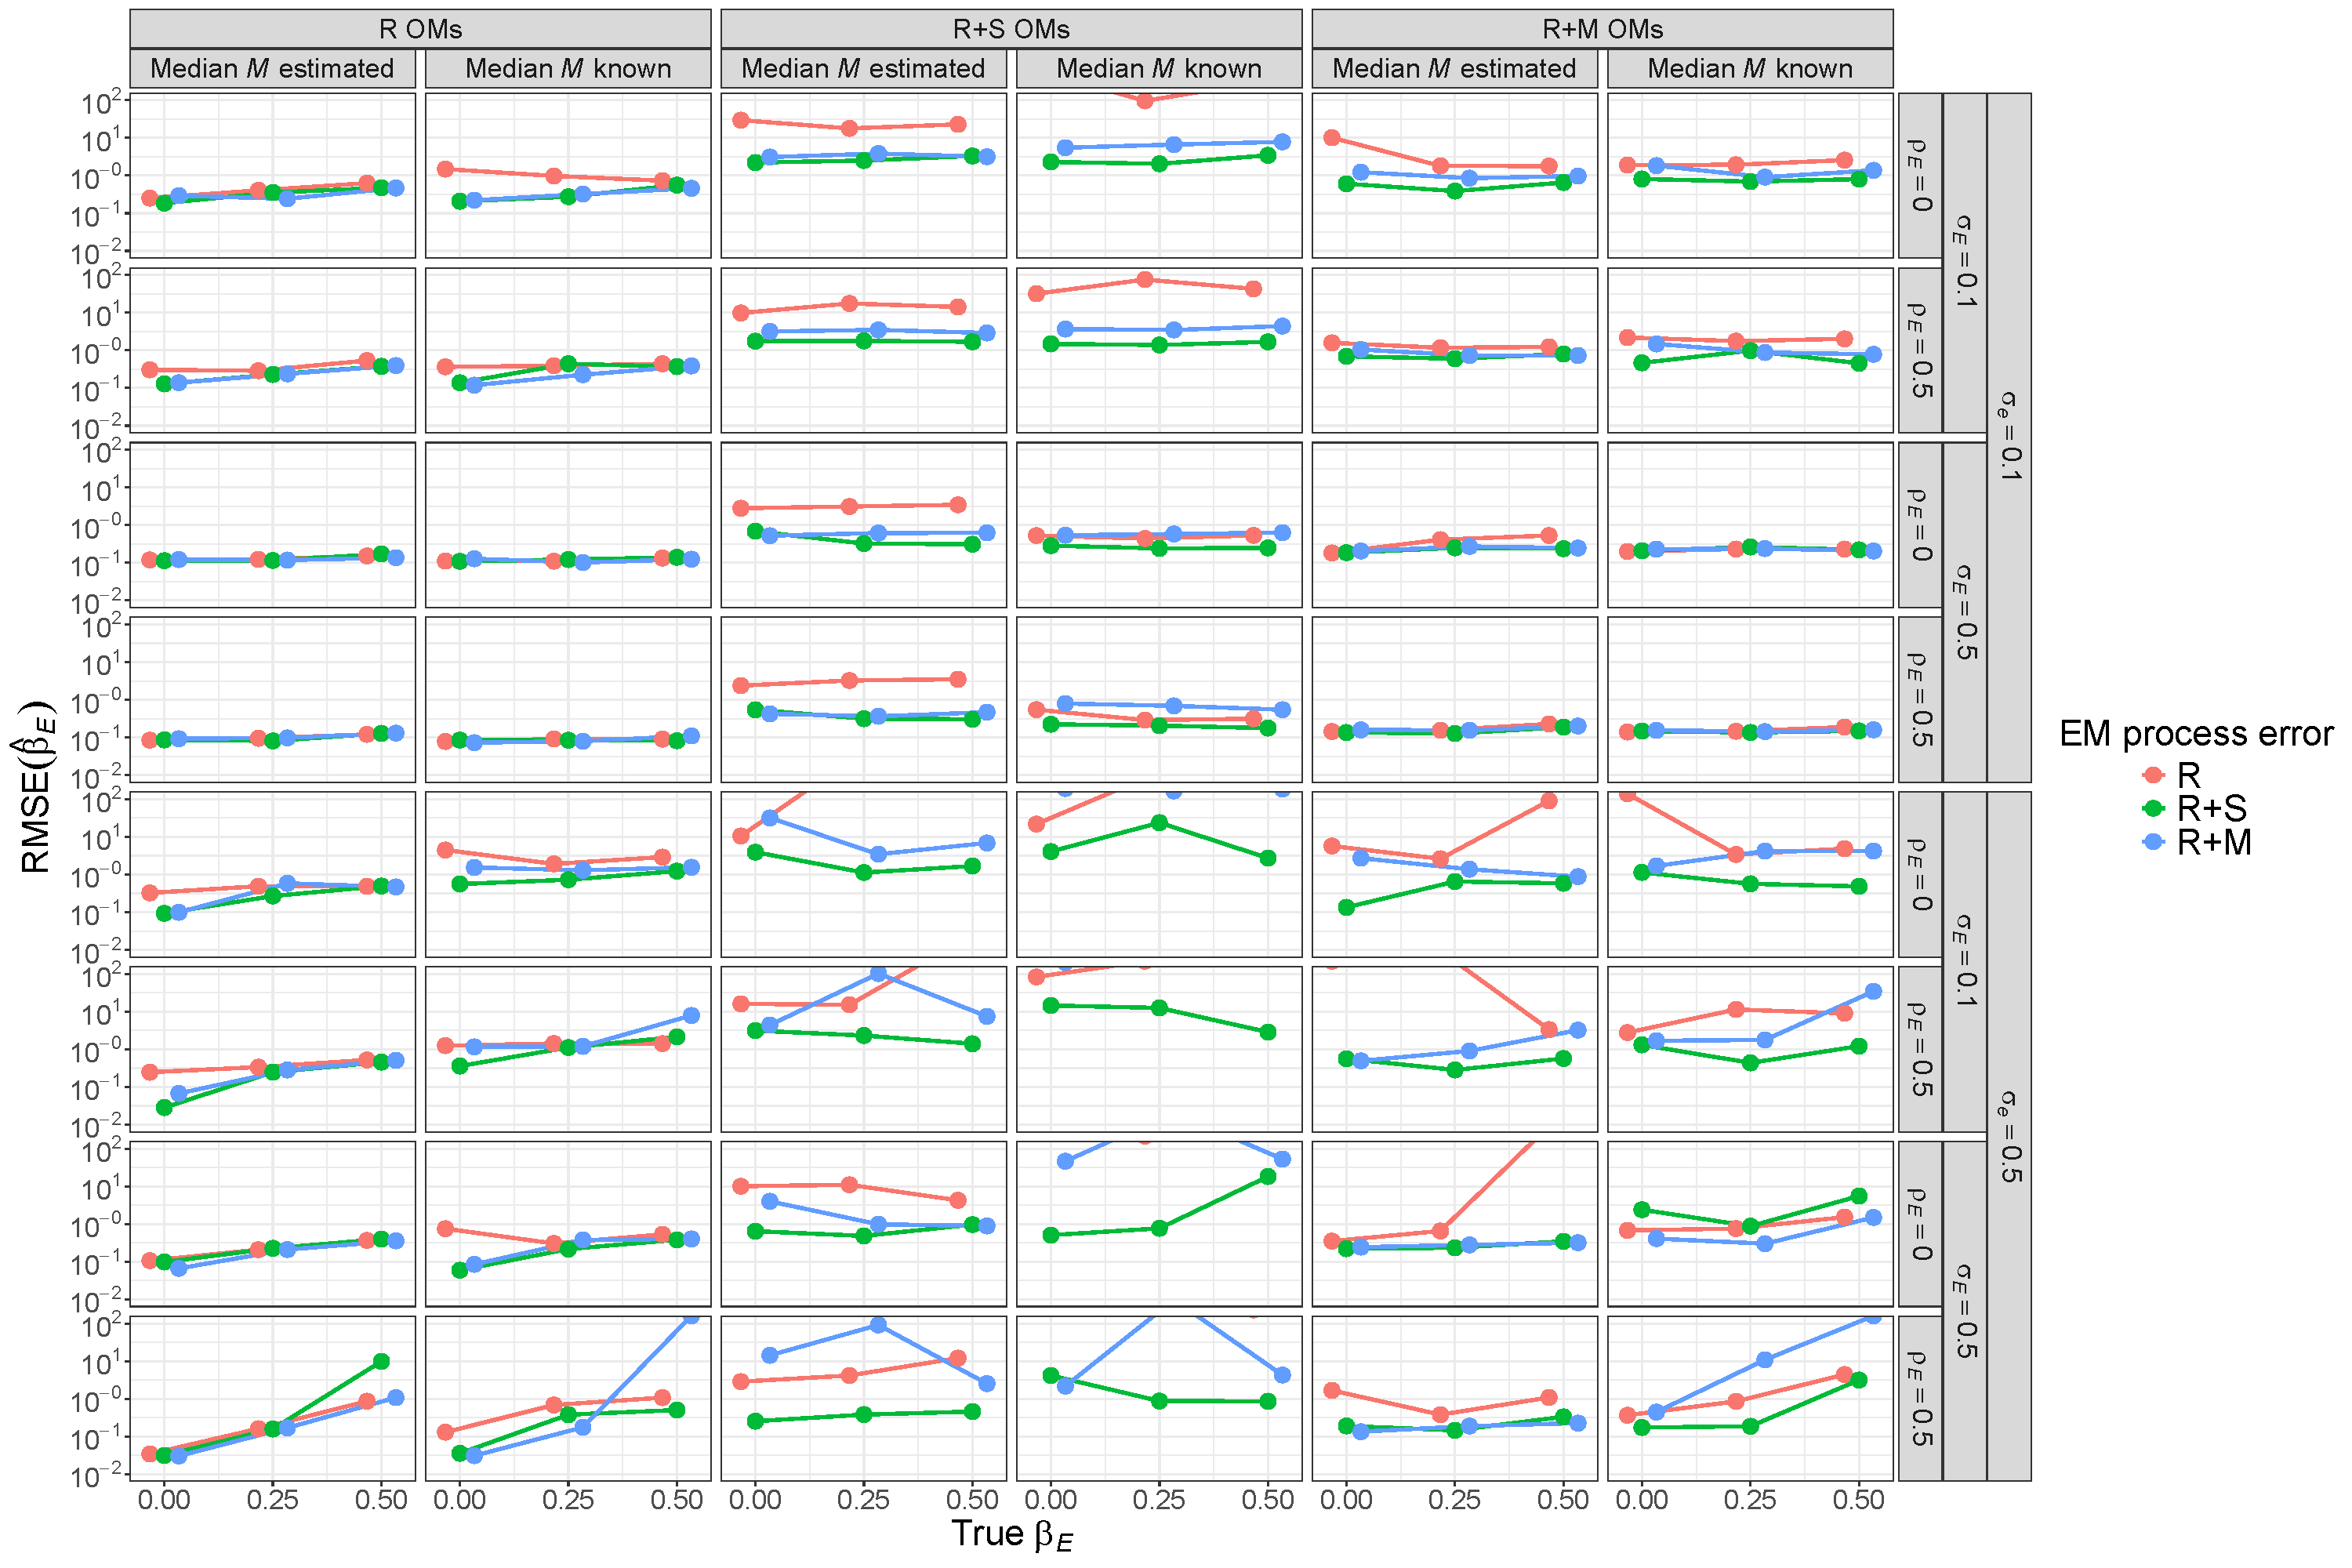
\includegraphics[height = \textheight]{beta_E_rmse_main}
\end{center}
\caption{Root mean square error (RMSE) of estimates of covariate effect on natural mortality $\beta_E$ from fitting EMs with alternative process error assumptions and treatment of median natural mortality ($e^\beta_M$ known or estimated). All OMs had low observation error and contrast in fishing mortality.}\label{beta_E_rmse}
\end{figure}
\end{landscape}

\begin{landscape}
\begin{figure}
\begin{center}
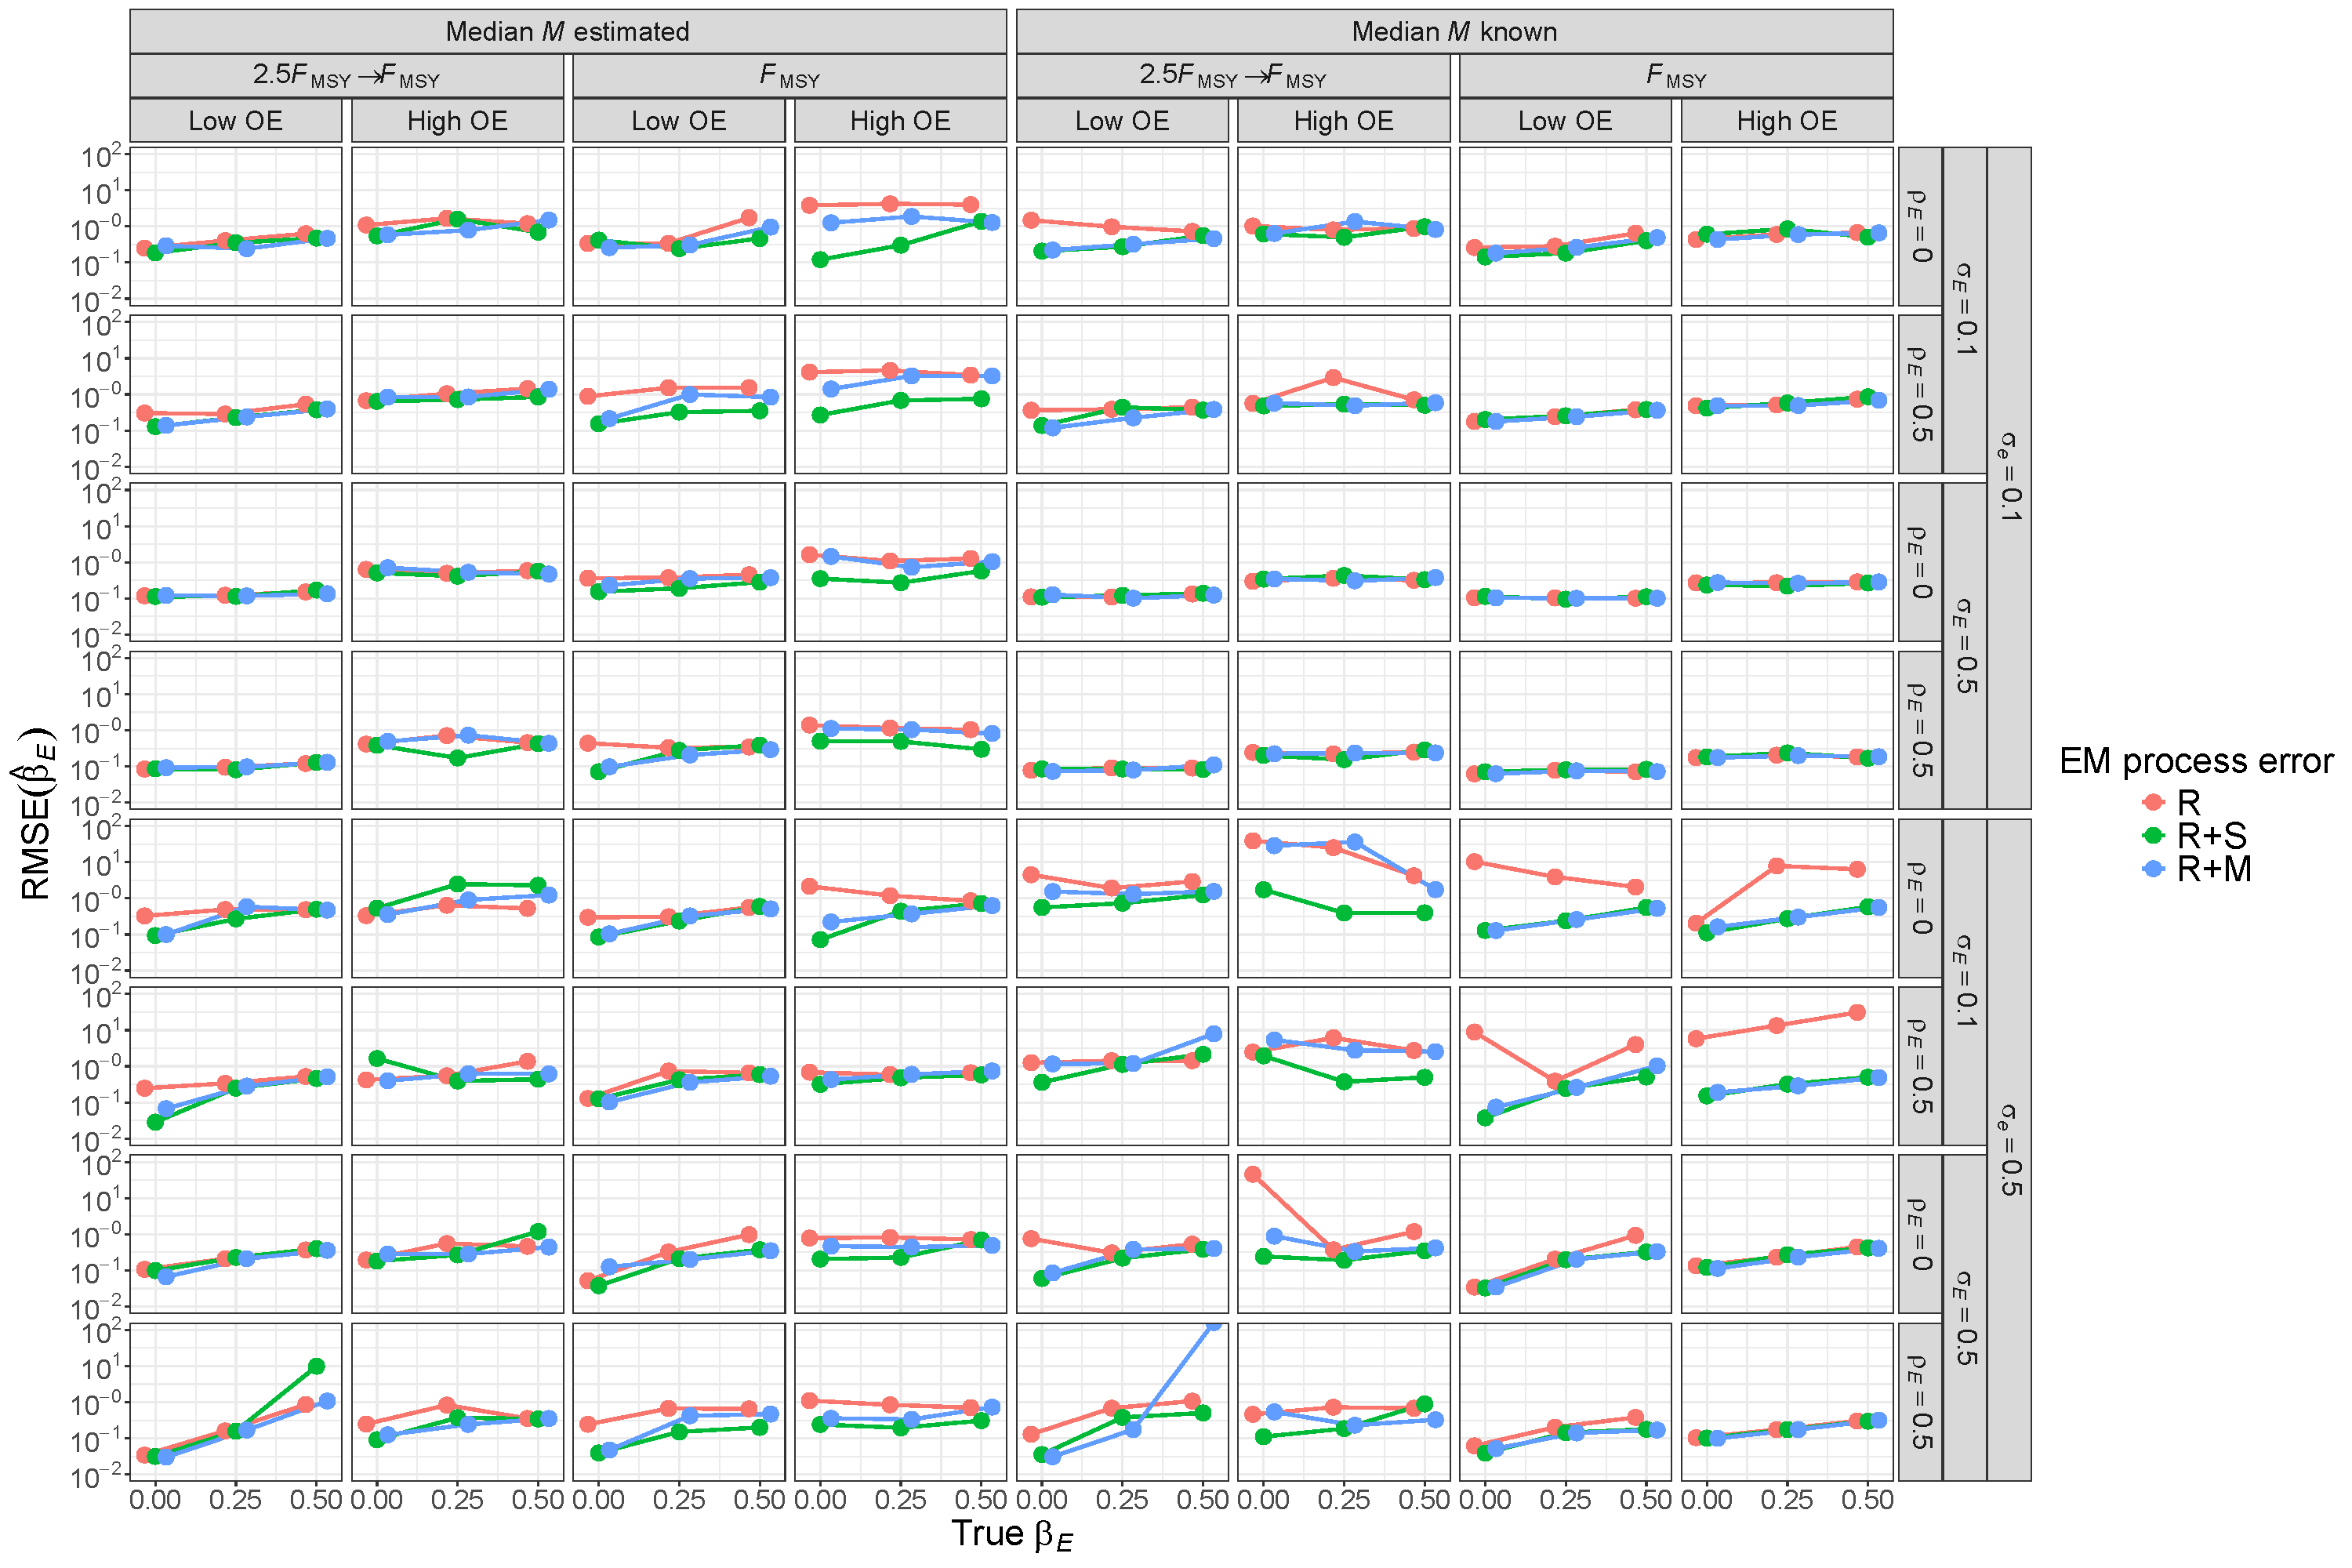
\includegraphics[height = \textheight]{beta_E_rmse_Rom}
\end{center}
\caption{For R OMs, root mean square error (RMSE) of estimates of covariate effect on natural mortality $\beta_E$ from fitting EMs with alternative process error assumptions and treatment of median natural mortality ($e^\beta_M$ known or estimated). }\label{beta_E_rmse_Rom}
\end{figure}
\end{landscape}

\begin{landscape}
\begin{figure}
\begin{center}
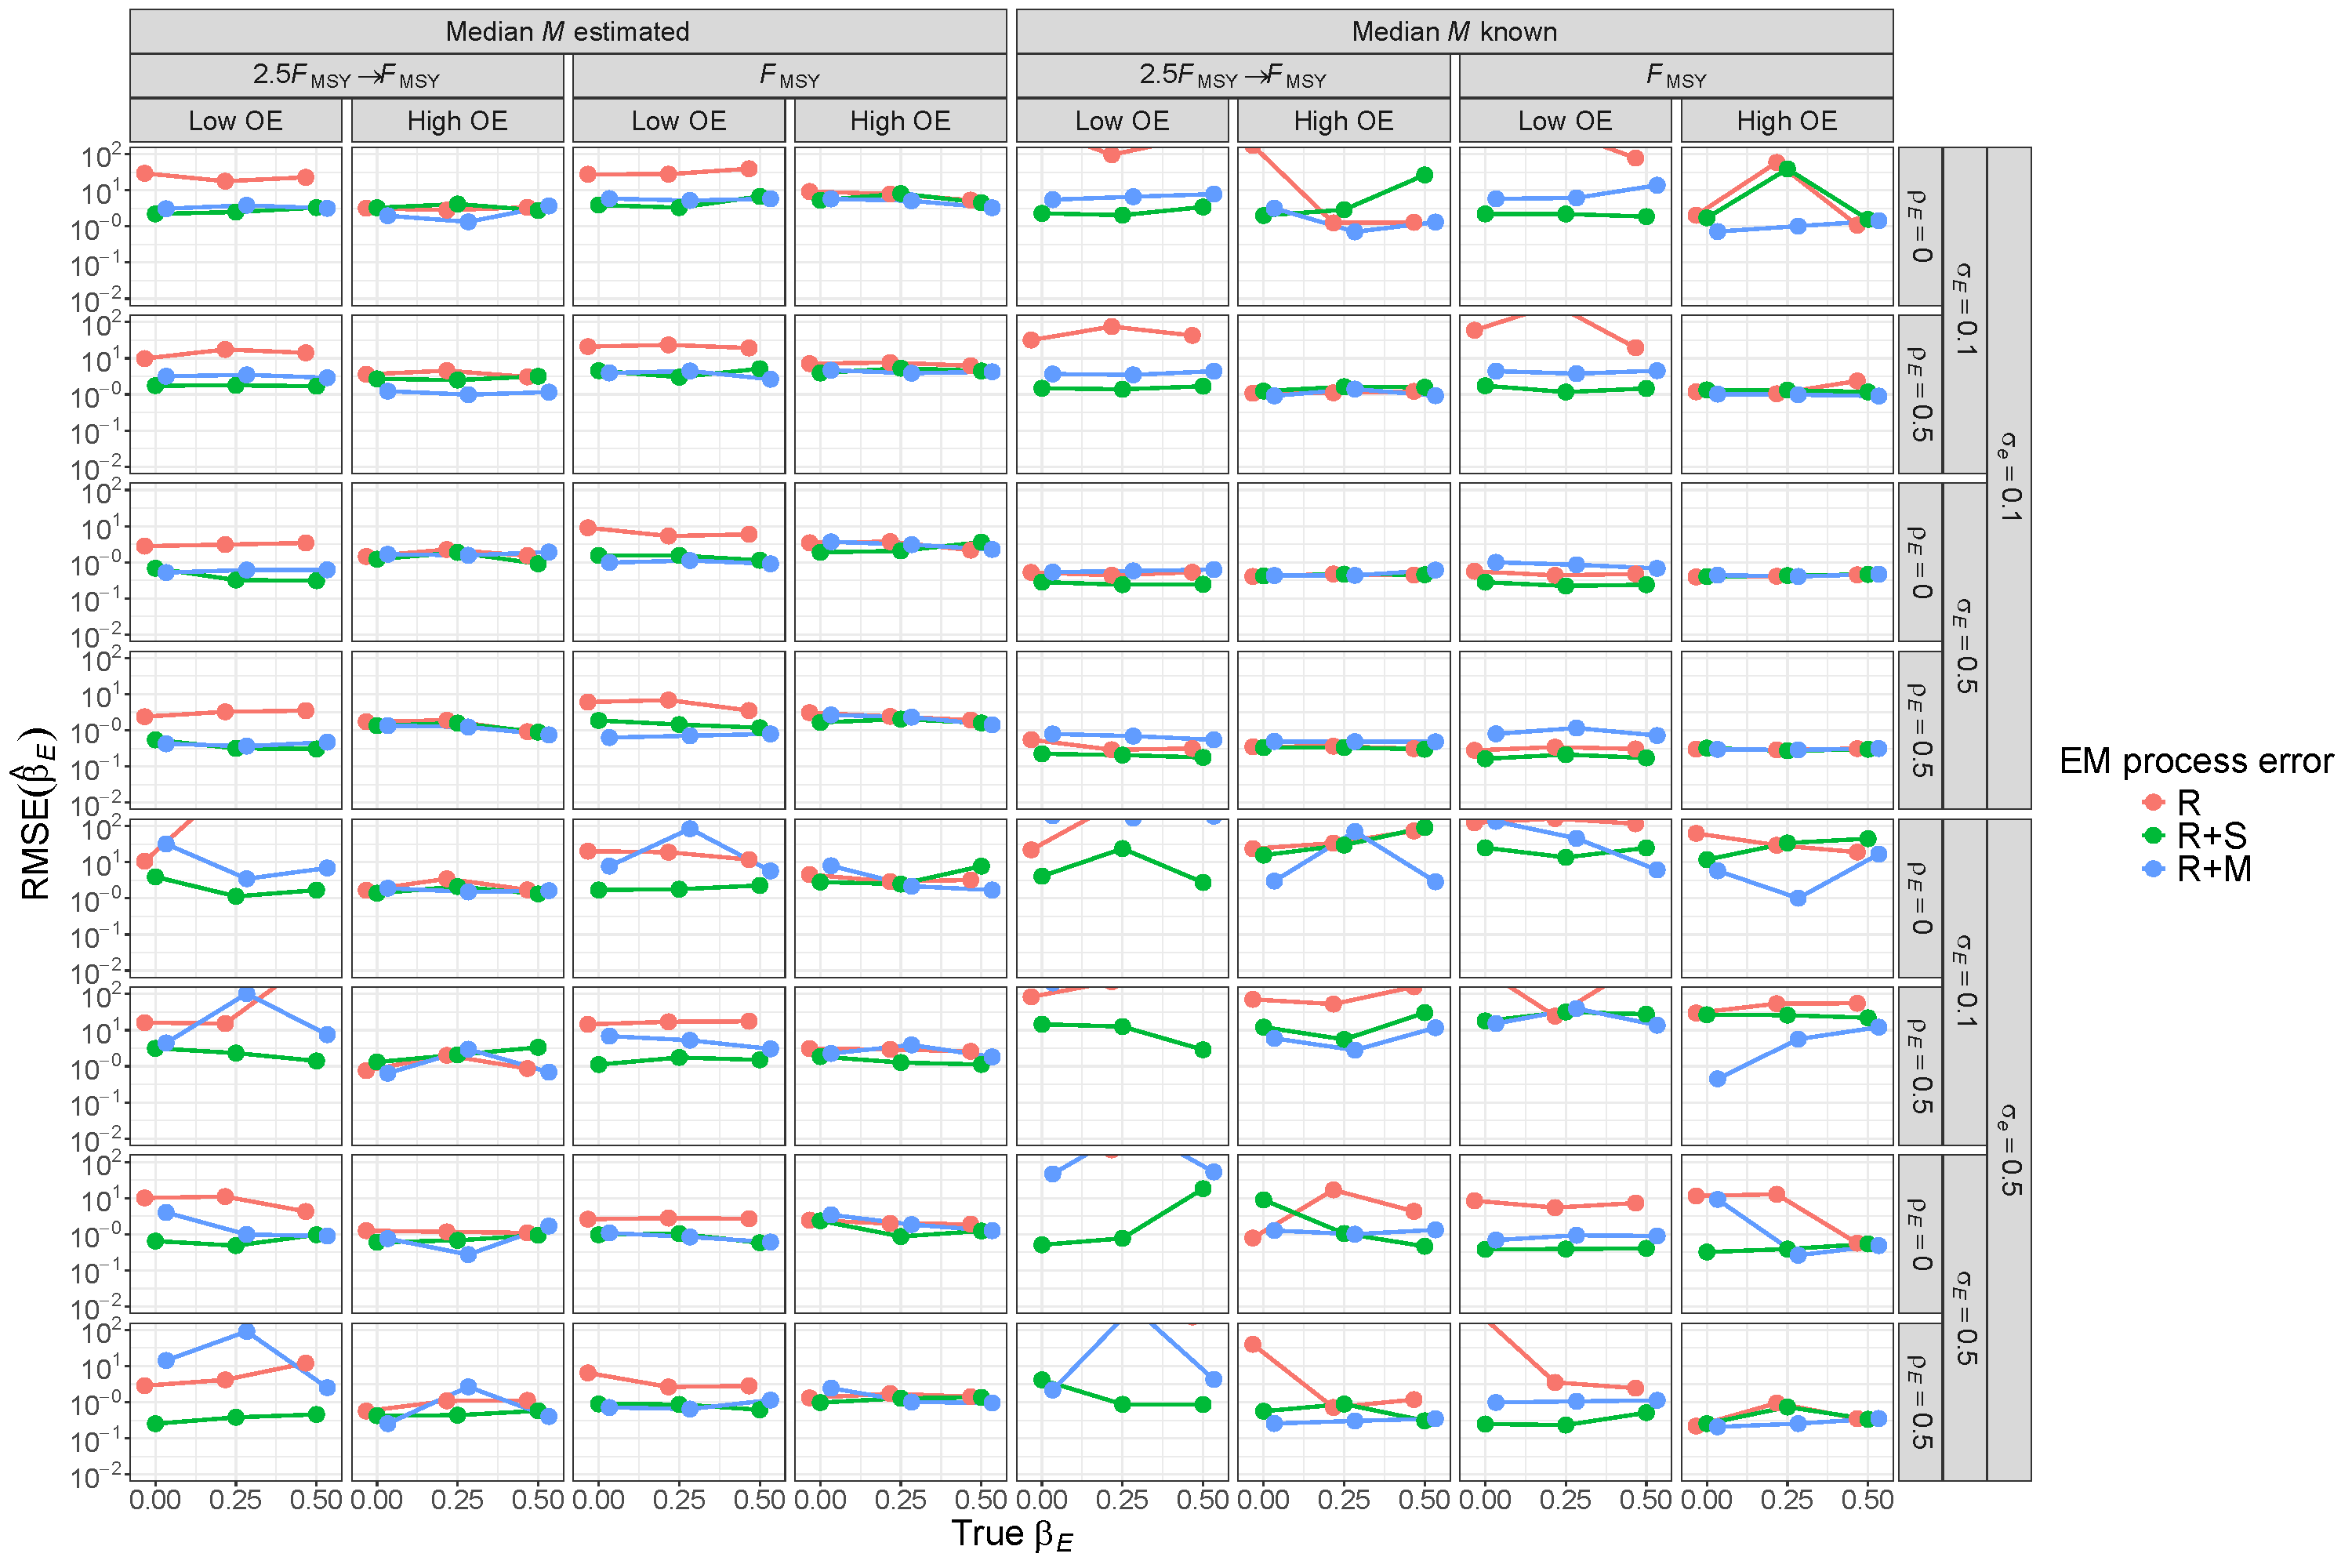
\includegraphics[height = \textheight]{beta_E_rmse_RSom}
\end{center}
\caption{For R+S OMs, root mean square error (RMSE) of estimates of covariate effect on natural mortality $\beta_E$ from fitting EMs with alternative process error assumptions and treatment of median natural mortality ($e^\beta_M$ known or estimated). }\label{beta_E_rmse_RSom}
\end{figure}
\end{landscape}

\begin{landscape}
\begin{figure}
\begin{center}
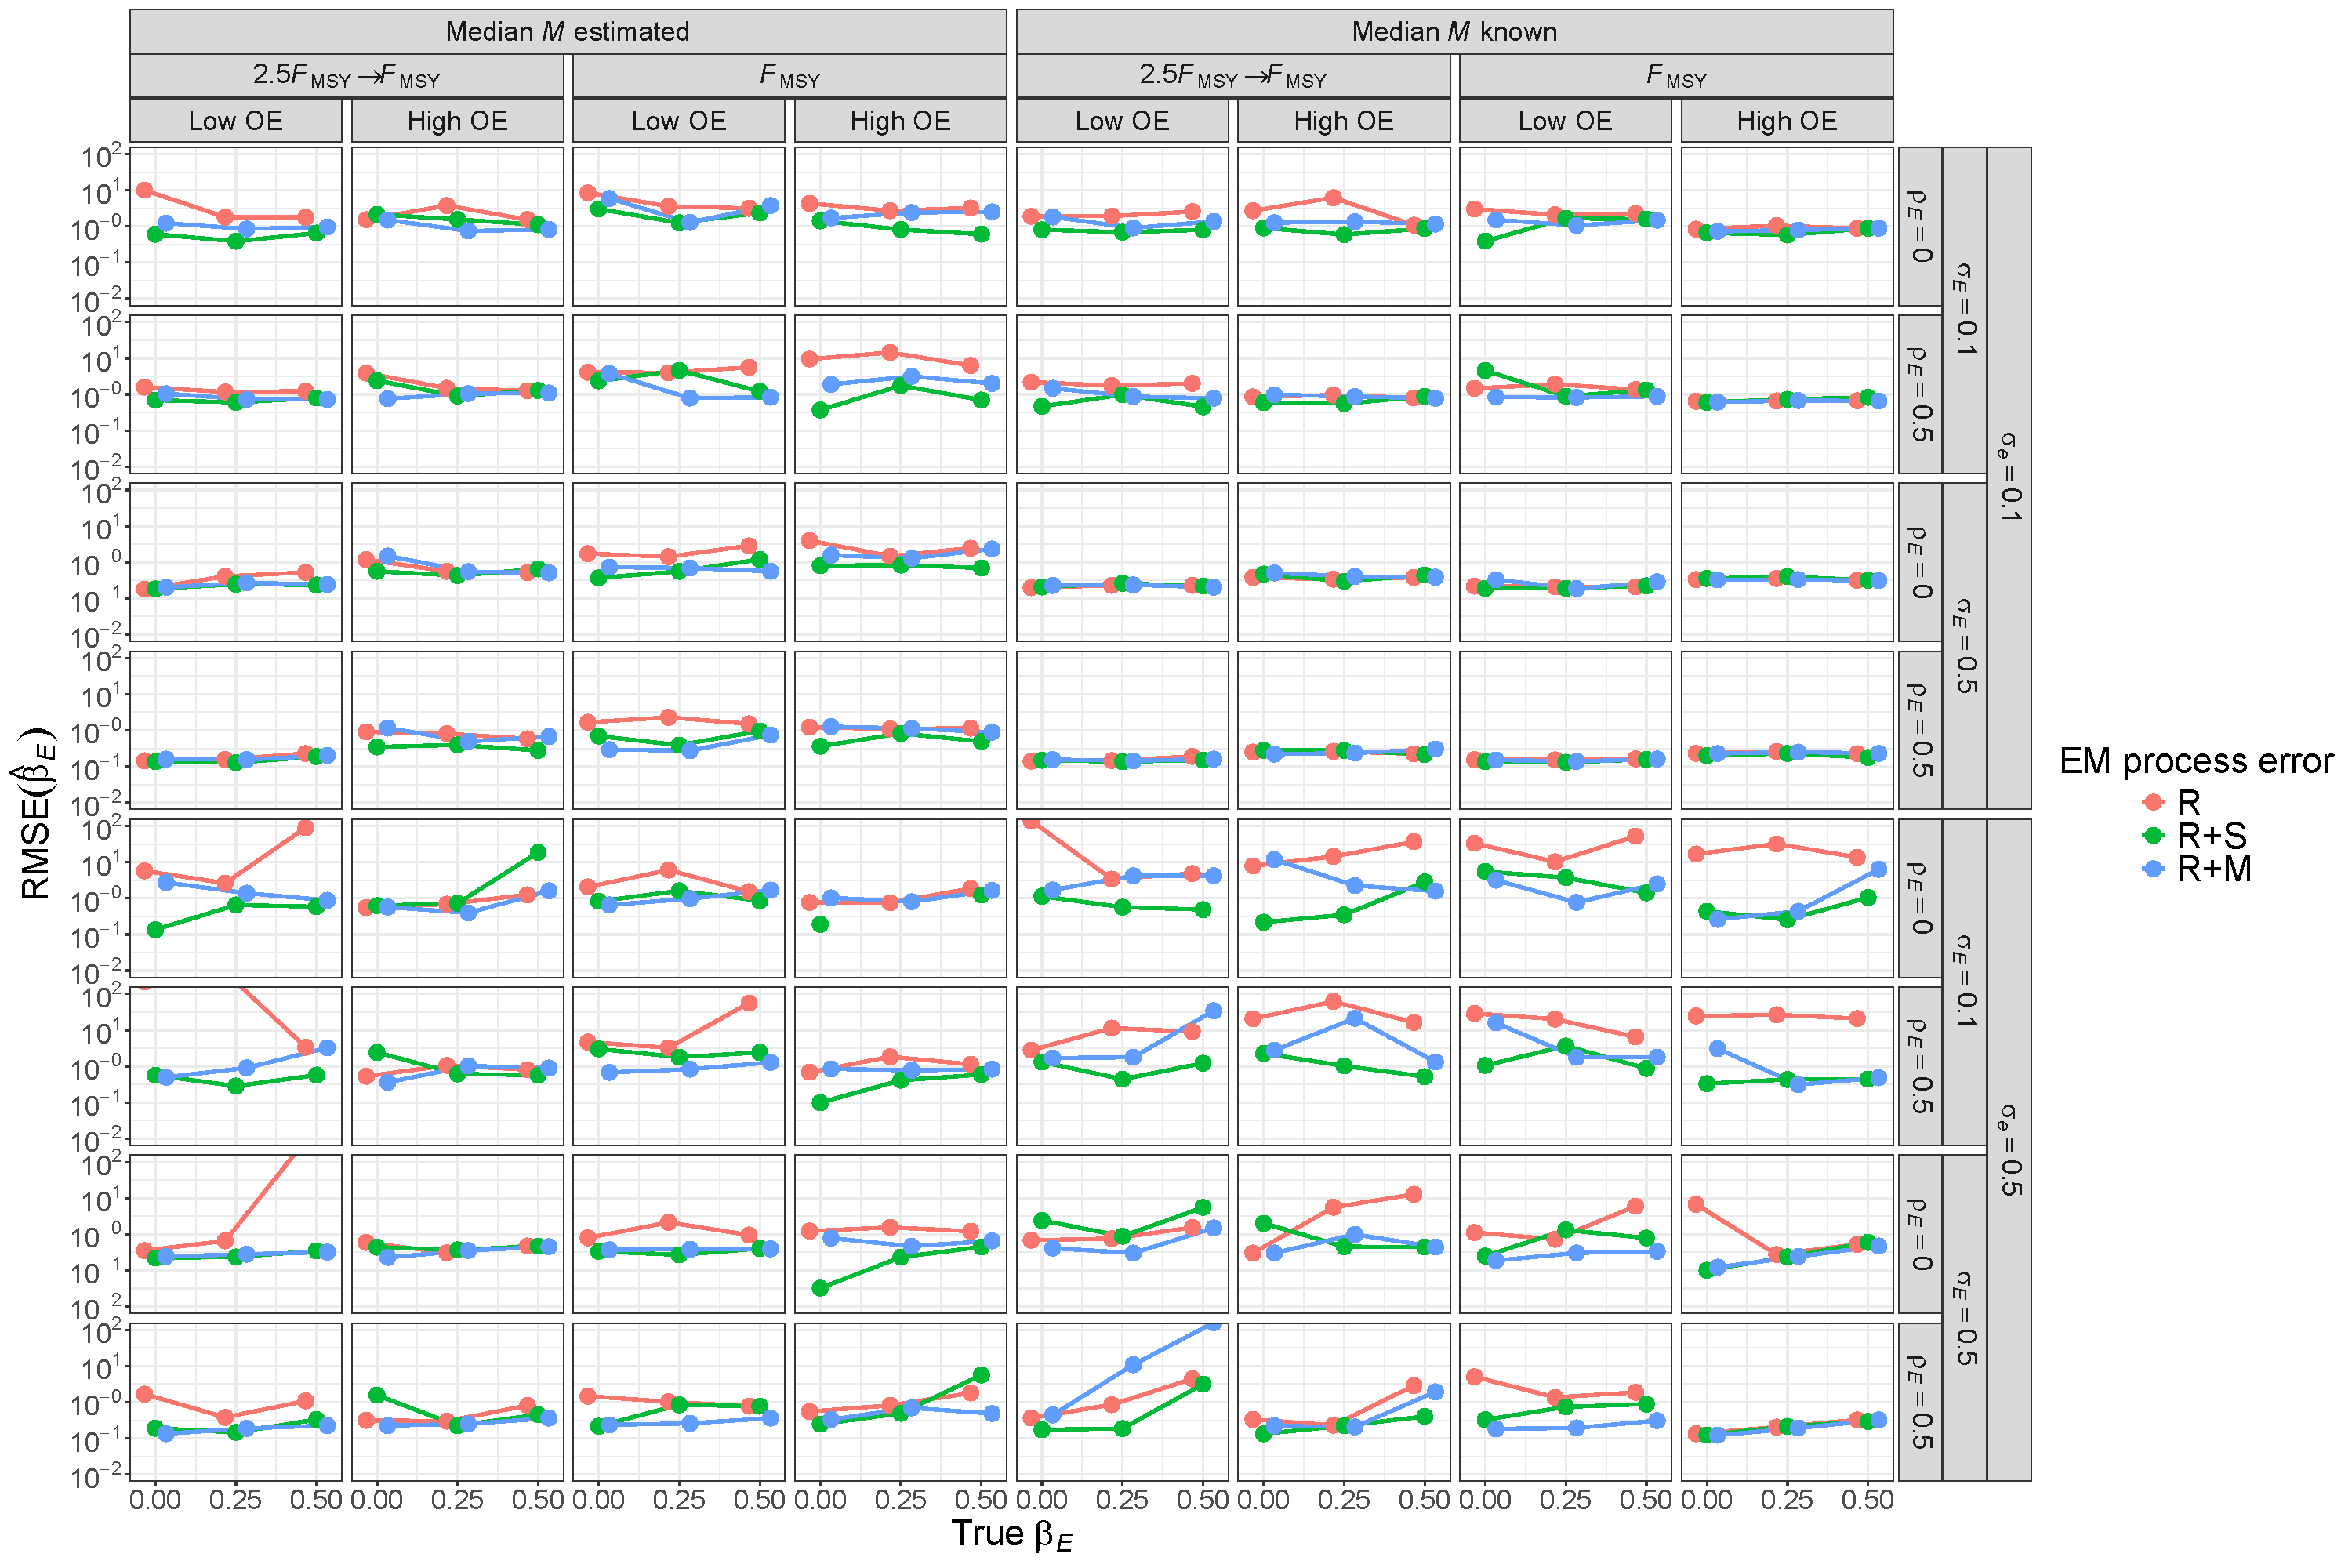
\includegraphics[height = \textheight]{beta_E_rmse_RMom}
\end{center}
\caption{For R+M OMs, root mean square error (RMSE) of estimates of covariate effect on natural mortality $\beta_E$ from fitting EMs with alternative process error assumptions and treatment of median natural mortality ($e^\beta_M$ known or estimated). }\label{beta_E_rmse_RMom}
\end{figure}
\end{landscape}

\hypertarget{covariate-effect-estimate-and-standard-error-example}{%
\subsection*{Covariate effect estimate and standard error example}\label{covariate-effect-estimate-and-standard-error-example}}
\addcontentsline{toc}{subsection}{Covariate effect estimate and standard error example}

\begin{landscape}
\begin{figure}
\begin{center}
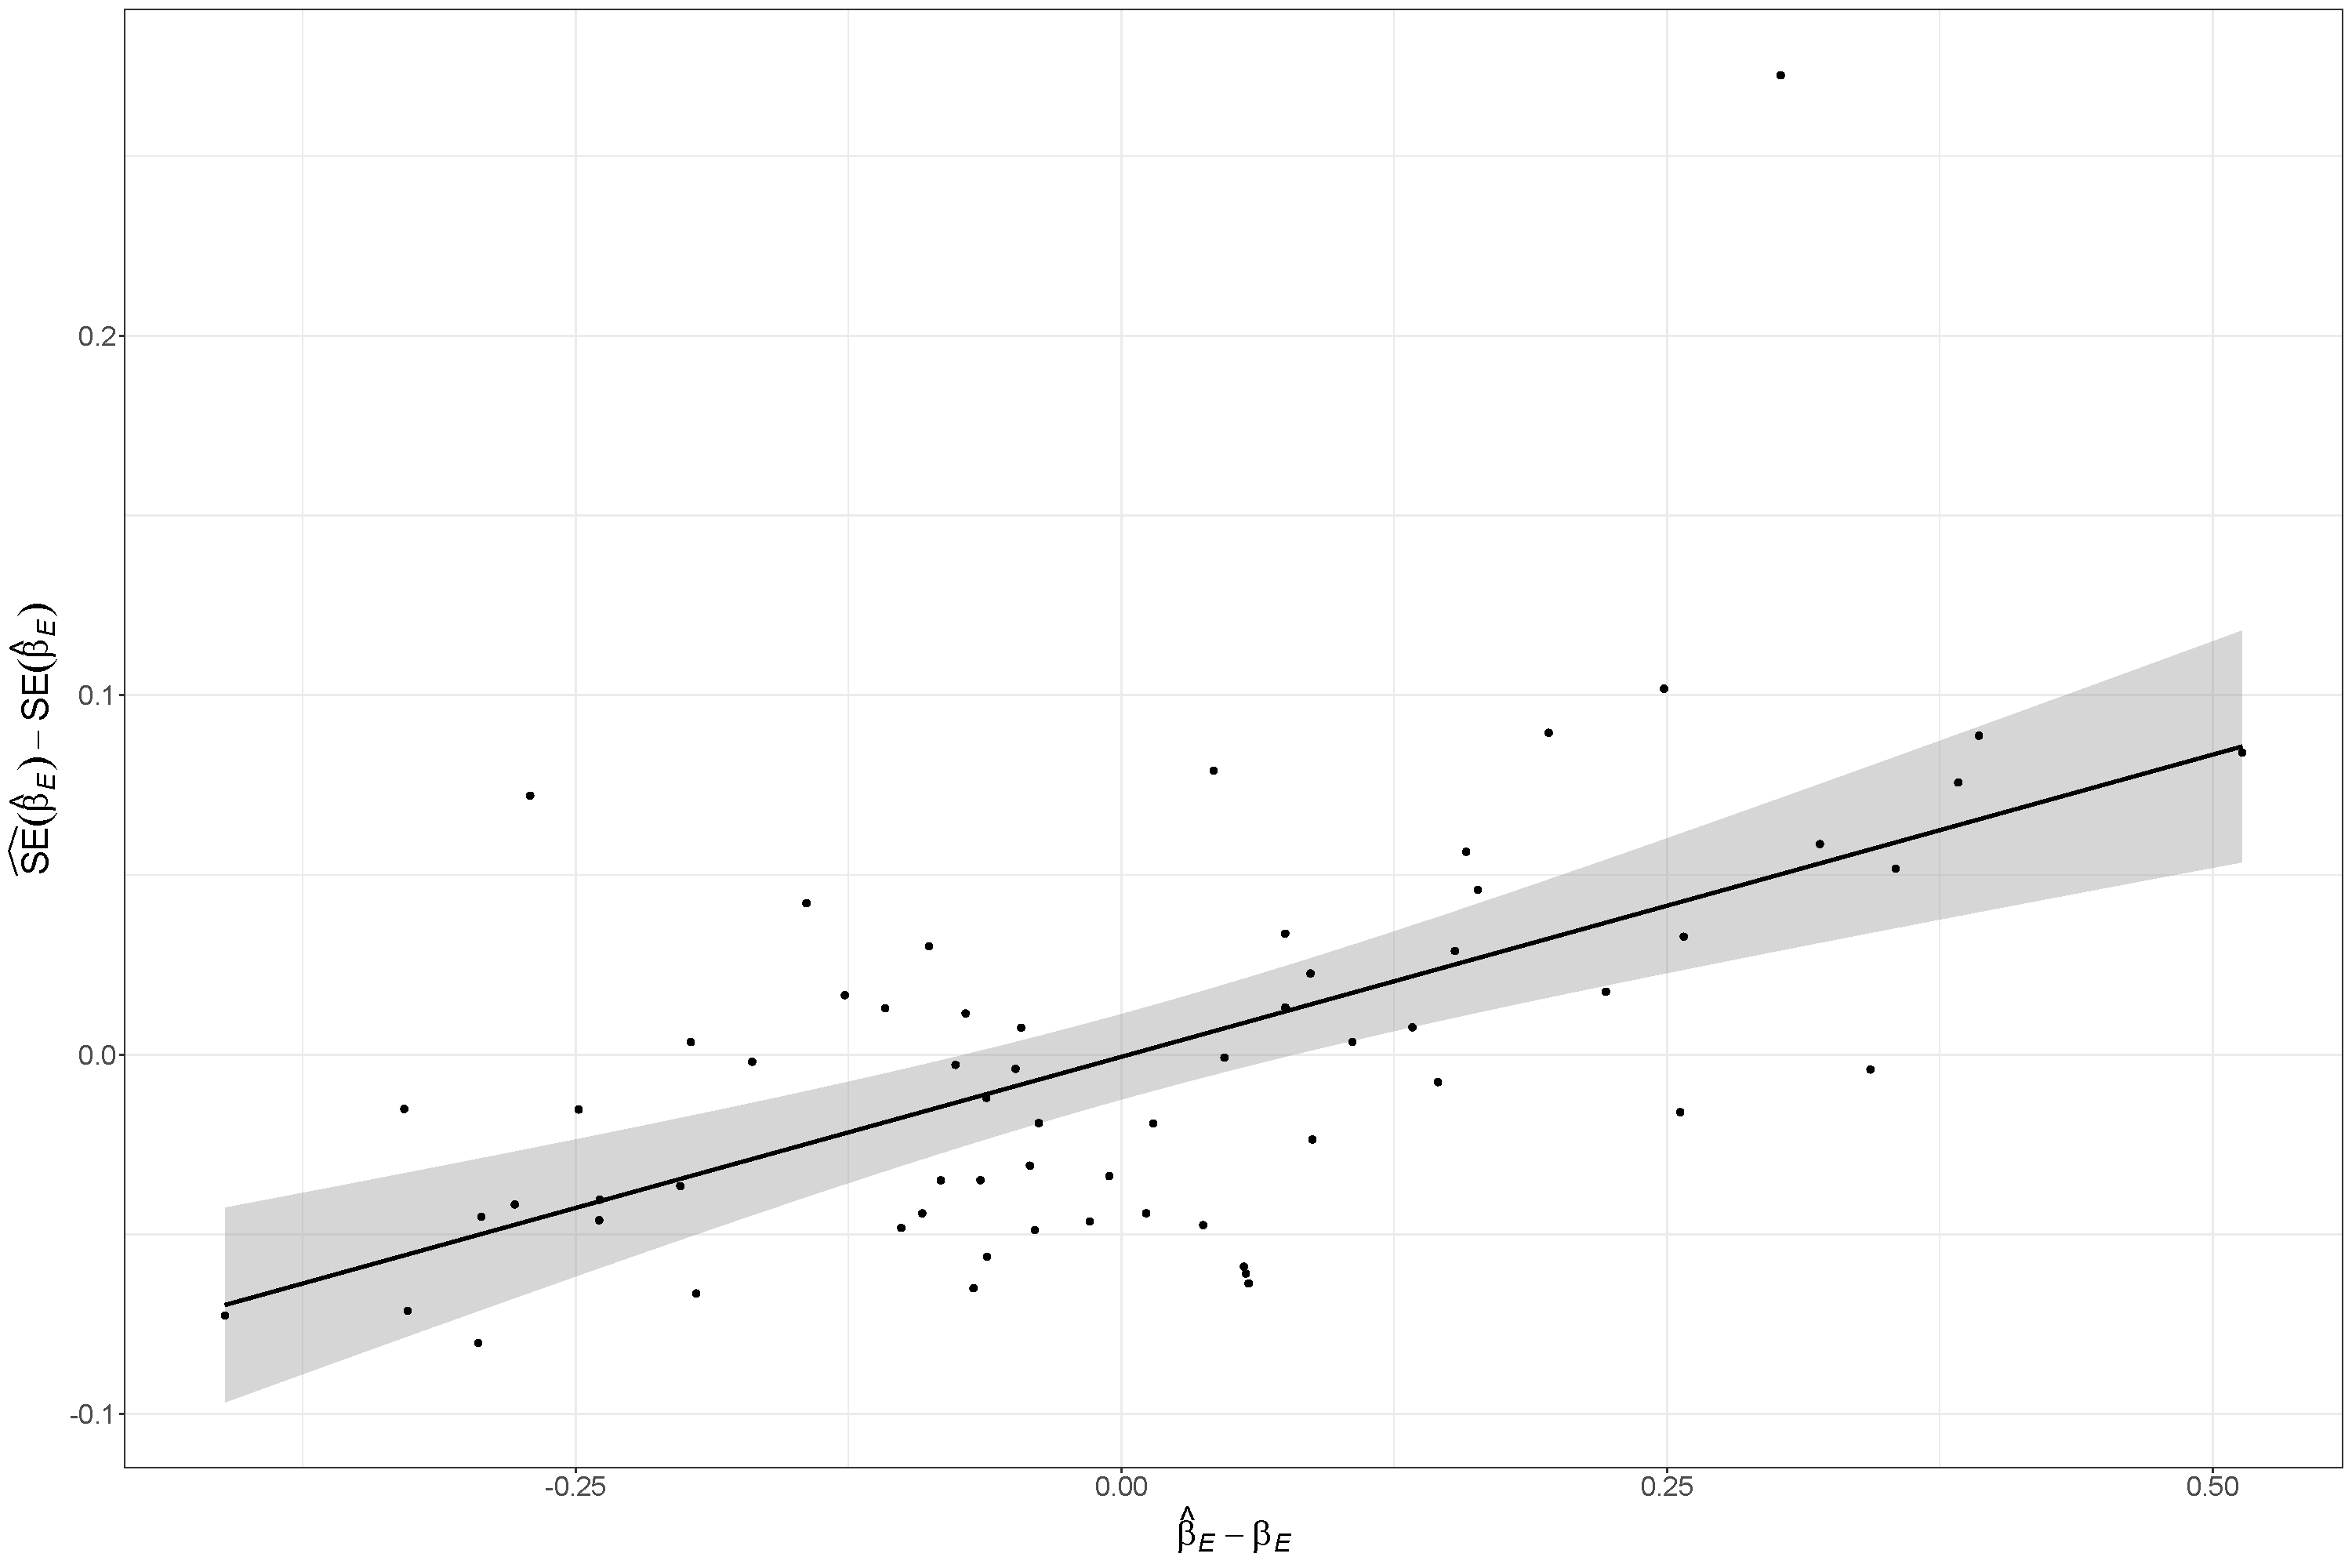
\includegraphics[height = \textheight]{om_69_em_5_beta_E_se_beta_E_lm_plot}
\end{center}
\caption{Positive correlation of covariate effect estimates and Hessian-based standard error estimates for EM that also estimates the median natural mortality parameter and has correct R+M process error assumption fitted to simulated data from the OM with R+M process errors, temporal contrast in fishing pressure, low observation uncertainty for both population ($Low OE$) and covariate observations ($\sigma_e = 0.1$), high and uncorrelated temporal variability in the true covariate ($\sigma_E = 0.5$ and $\rho_E = 0$), and the strongest covariate effect on natural mortality ($\beta_E = 0.5$).}\label{ex_lm_beta_E_SE_beta_E}
\end{figure}
\end{landscape}

\hypertarget{median-natural-mortality-parameter-bias}{%
\subsection*{Median Natural mortality parameter bias}\label{median-natural-mortality-parameter-bias}}
\addcontentsline{toc}{subsection}{Median Natural mortality parameter bias}

\begin{landscape}
\begin{figure}
\begin{center}
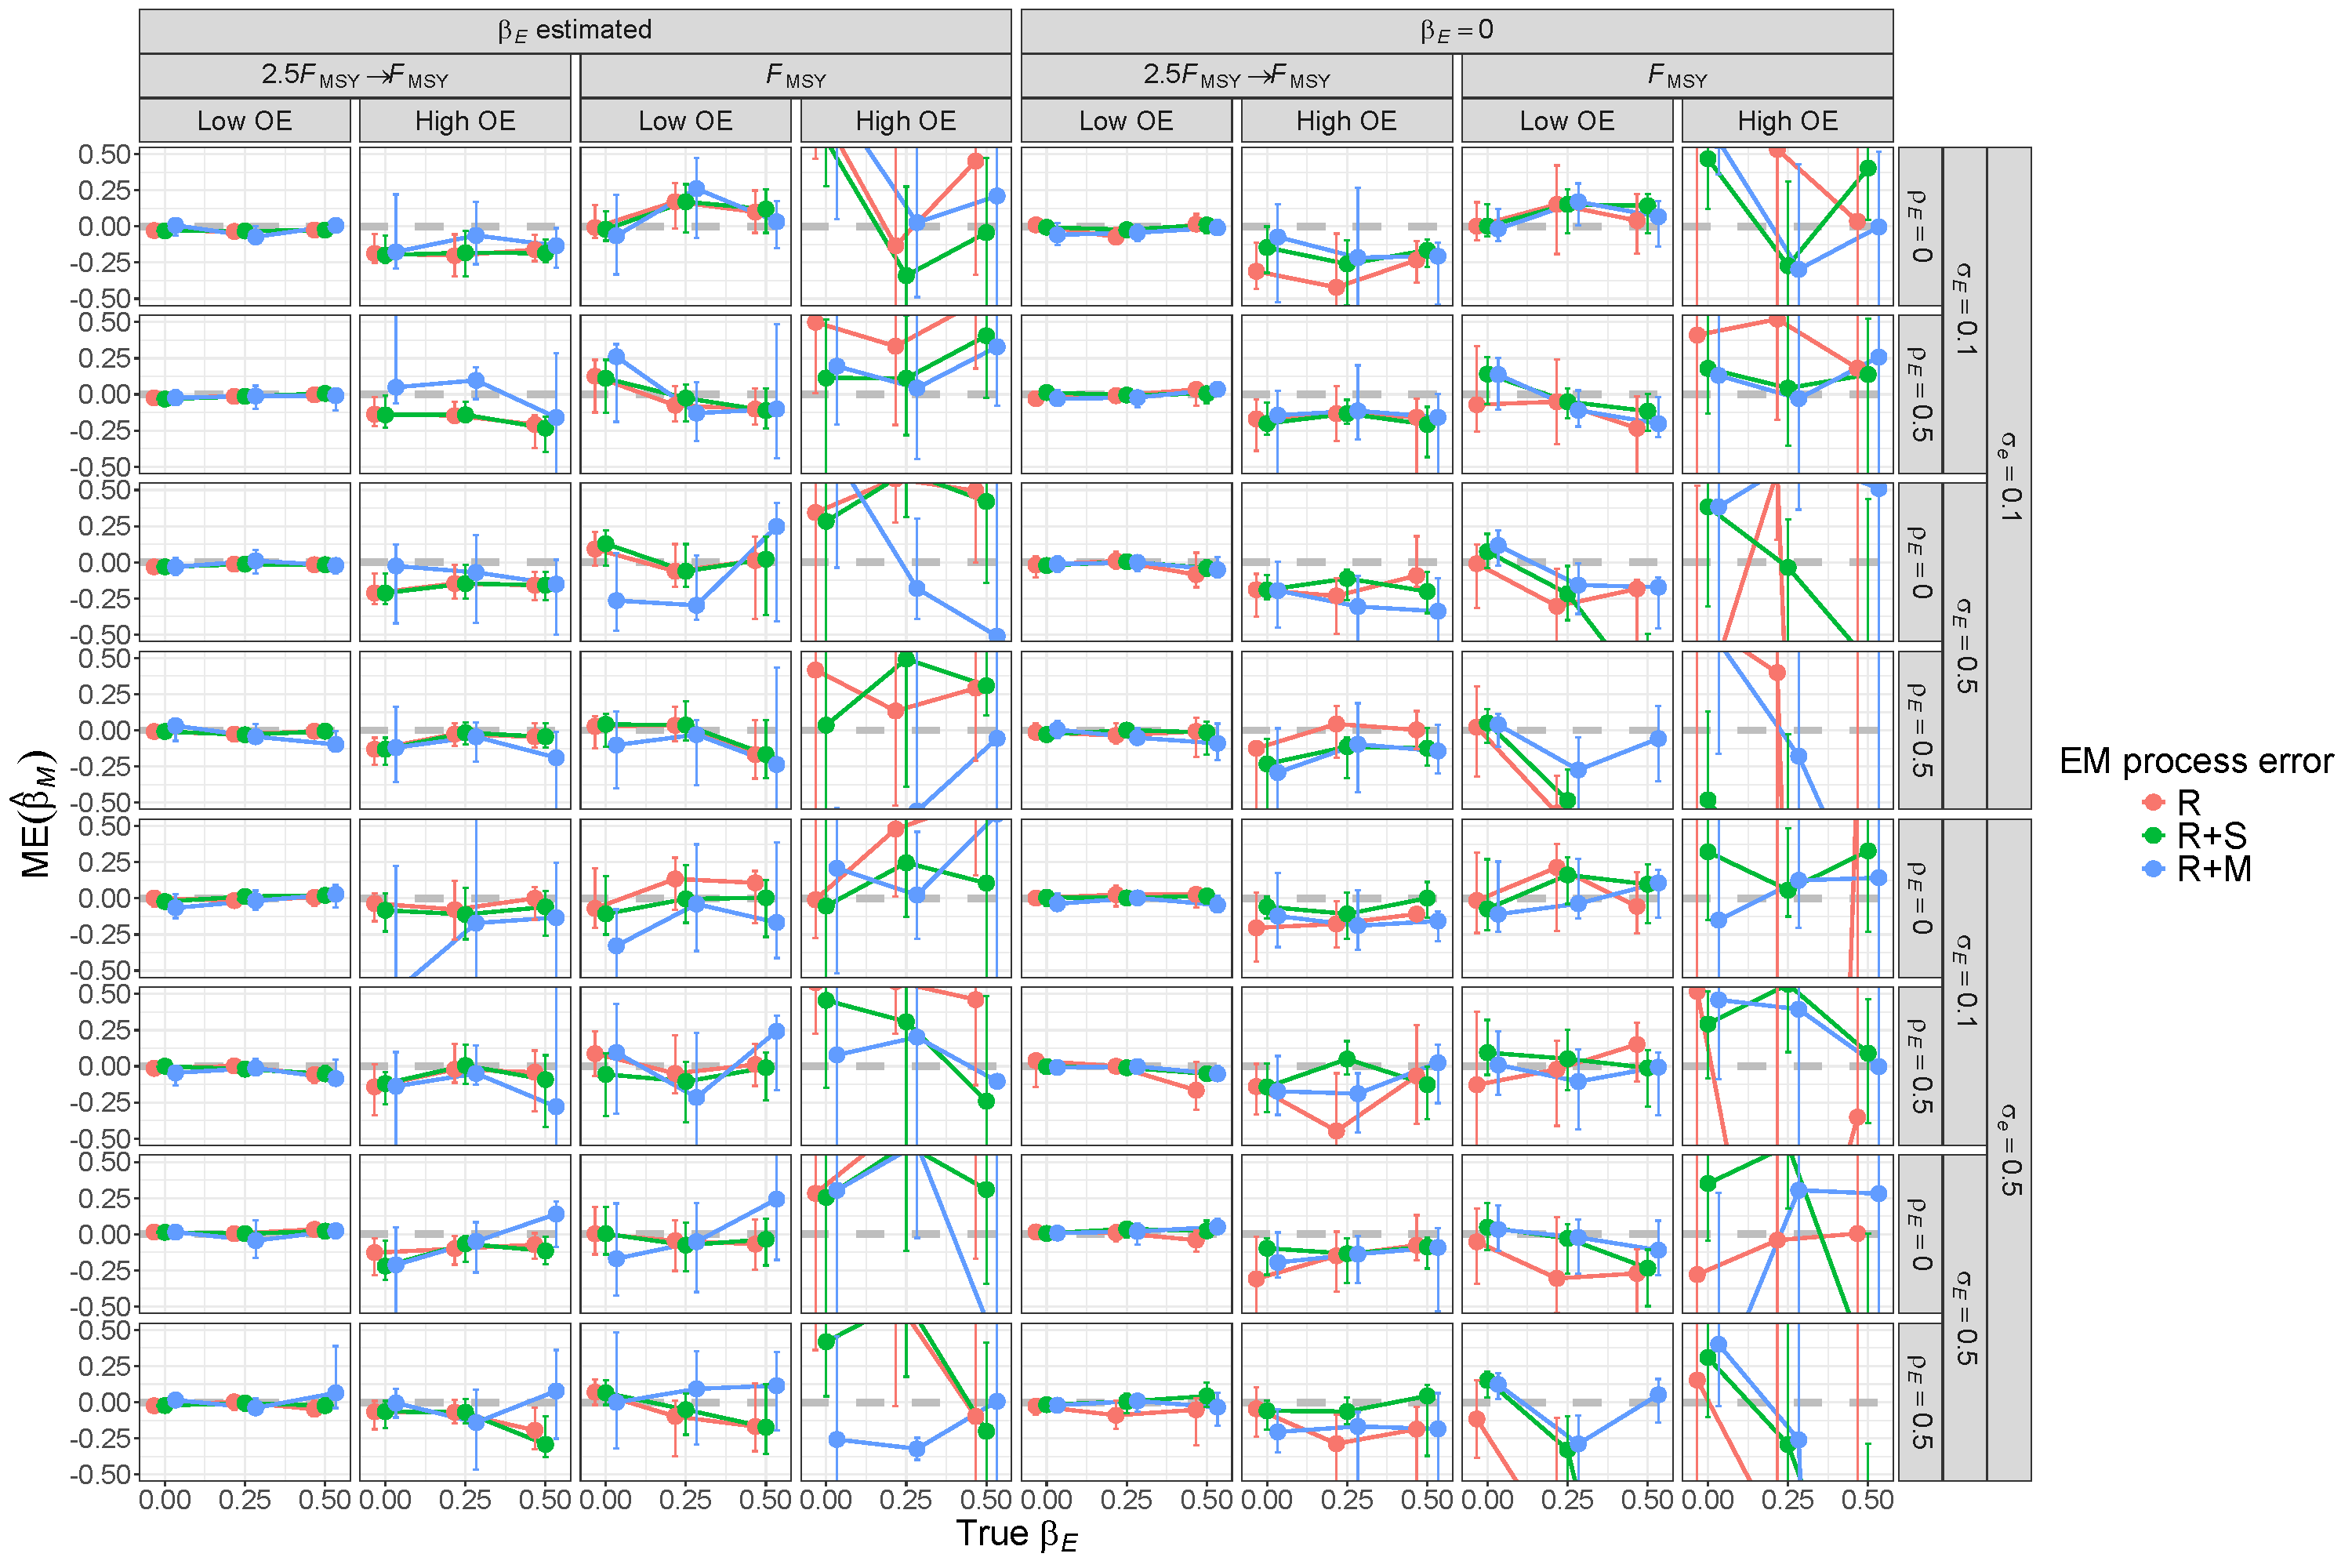
\includegraphics[height = \textheight]{beta_M_bias_Rom}
\end{center}
\caption{For R OMs, median error (ME) of estimates of $\beta_M$ from fitting EMs with alternative process error assumptions and treatment of covariate effect ($\beta_E = 0$ or estimated). Vertical lines represent 95\% confidence intervals.}\label{beta_M_bias_Rom}
\end{figure}
\end{landscape}

\begin{landscape}
\begin{figure}
\begin{center}
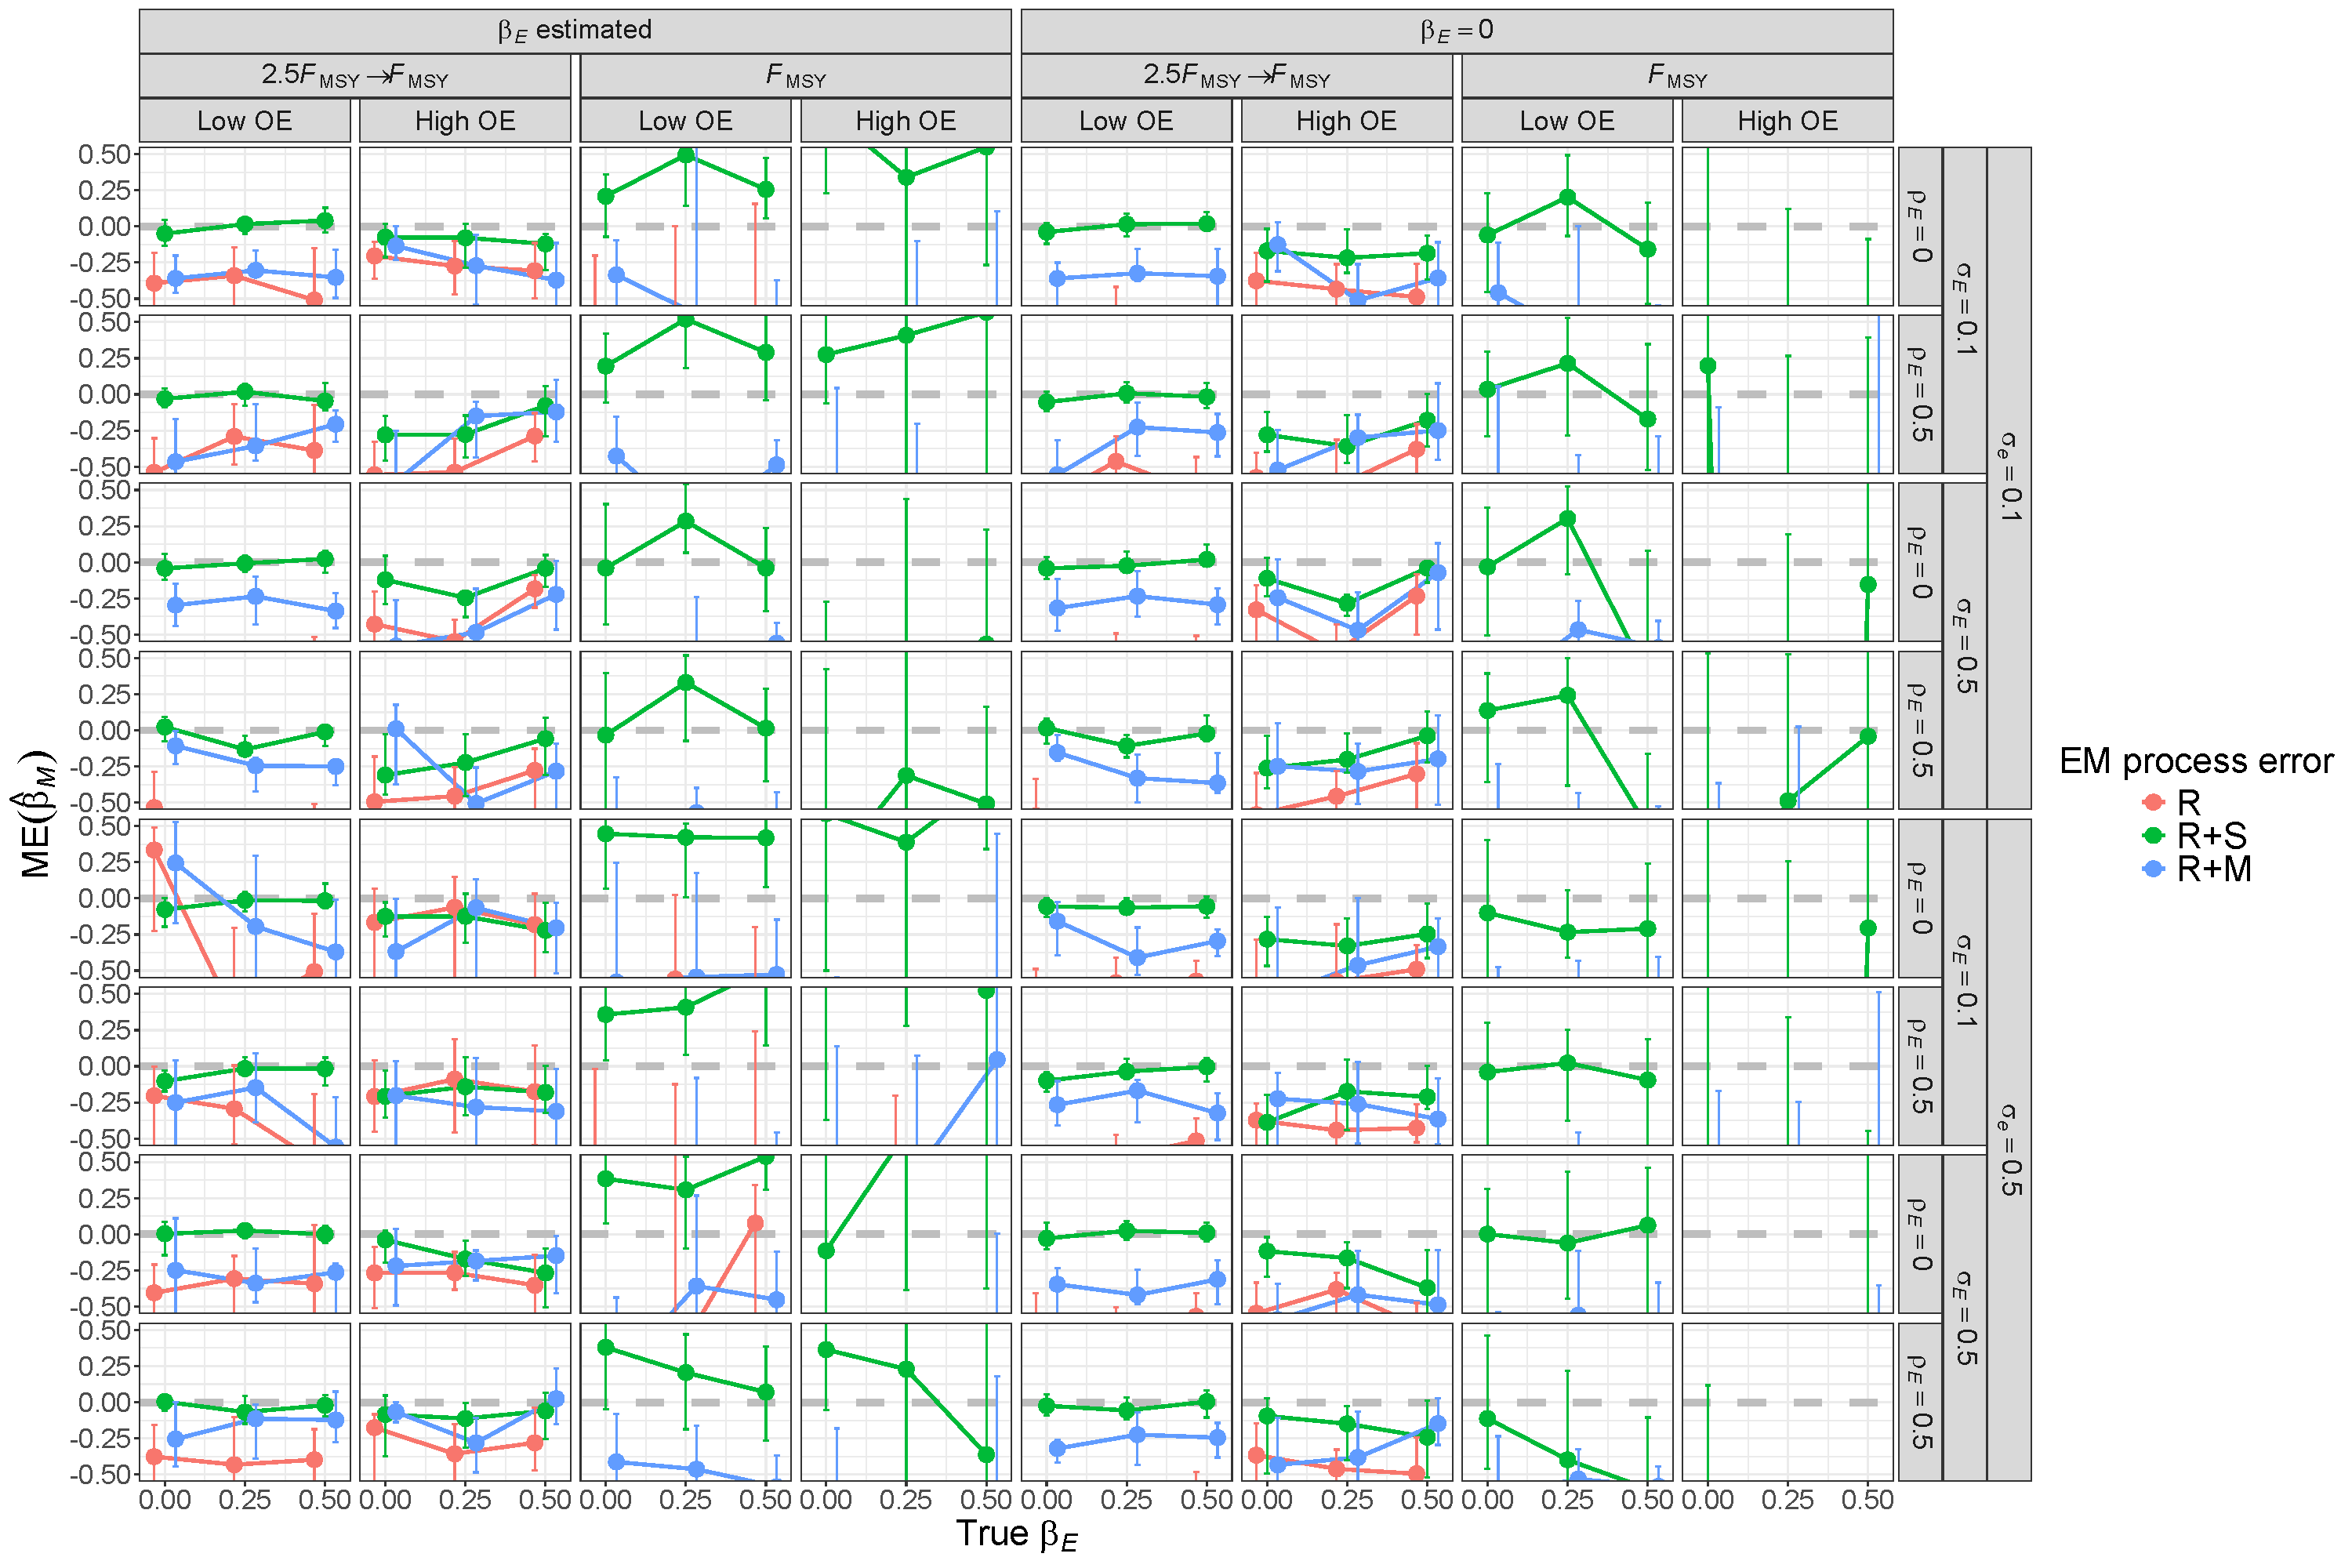
\includegraphics[height = \textheight]{beta_M_bias_RSom}
\end{center}
\caption{For R+S OMs, median error (ME) of estimates of $\beta_M$ from fitting EMs with alternative process error assumptions and treatment of covariate effect ($\beta_E = 0$ or estimated). Vertical lines represent 95\% confidence intervals.}\label{beta_M_bias_RSom}
\end{figure}
\end{landscape}

\begin{landscape}
\begin{figure}
\begin{center}
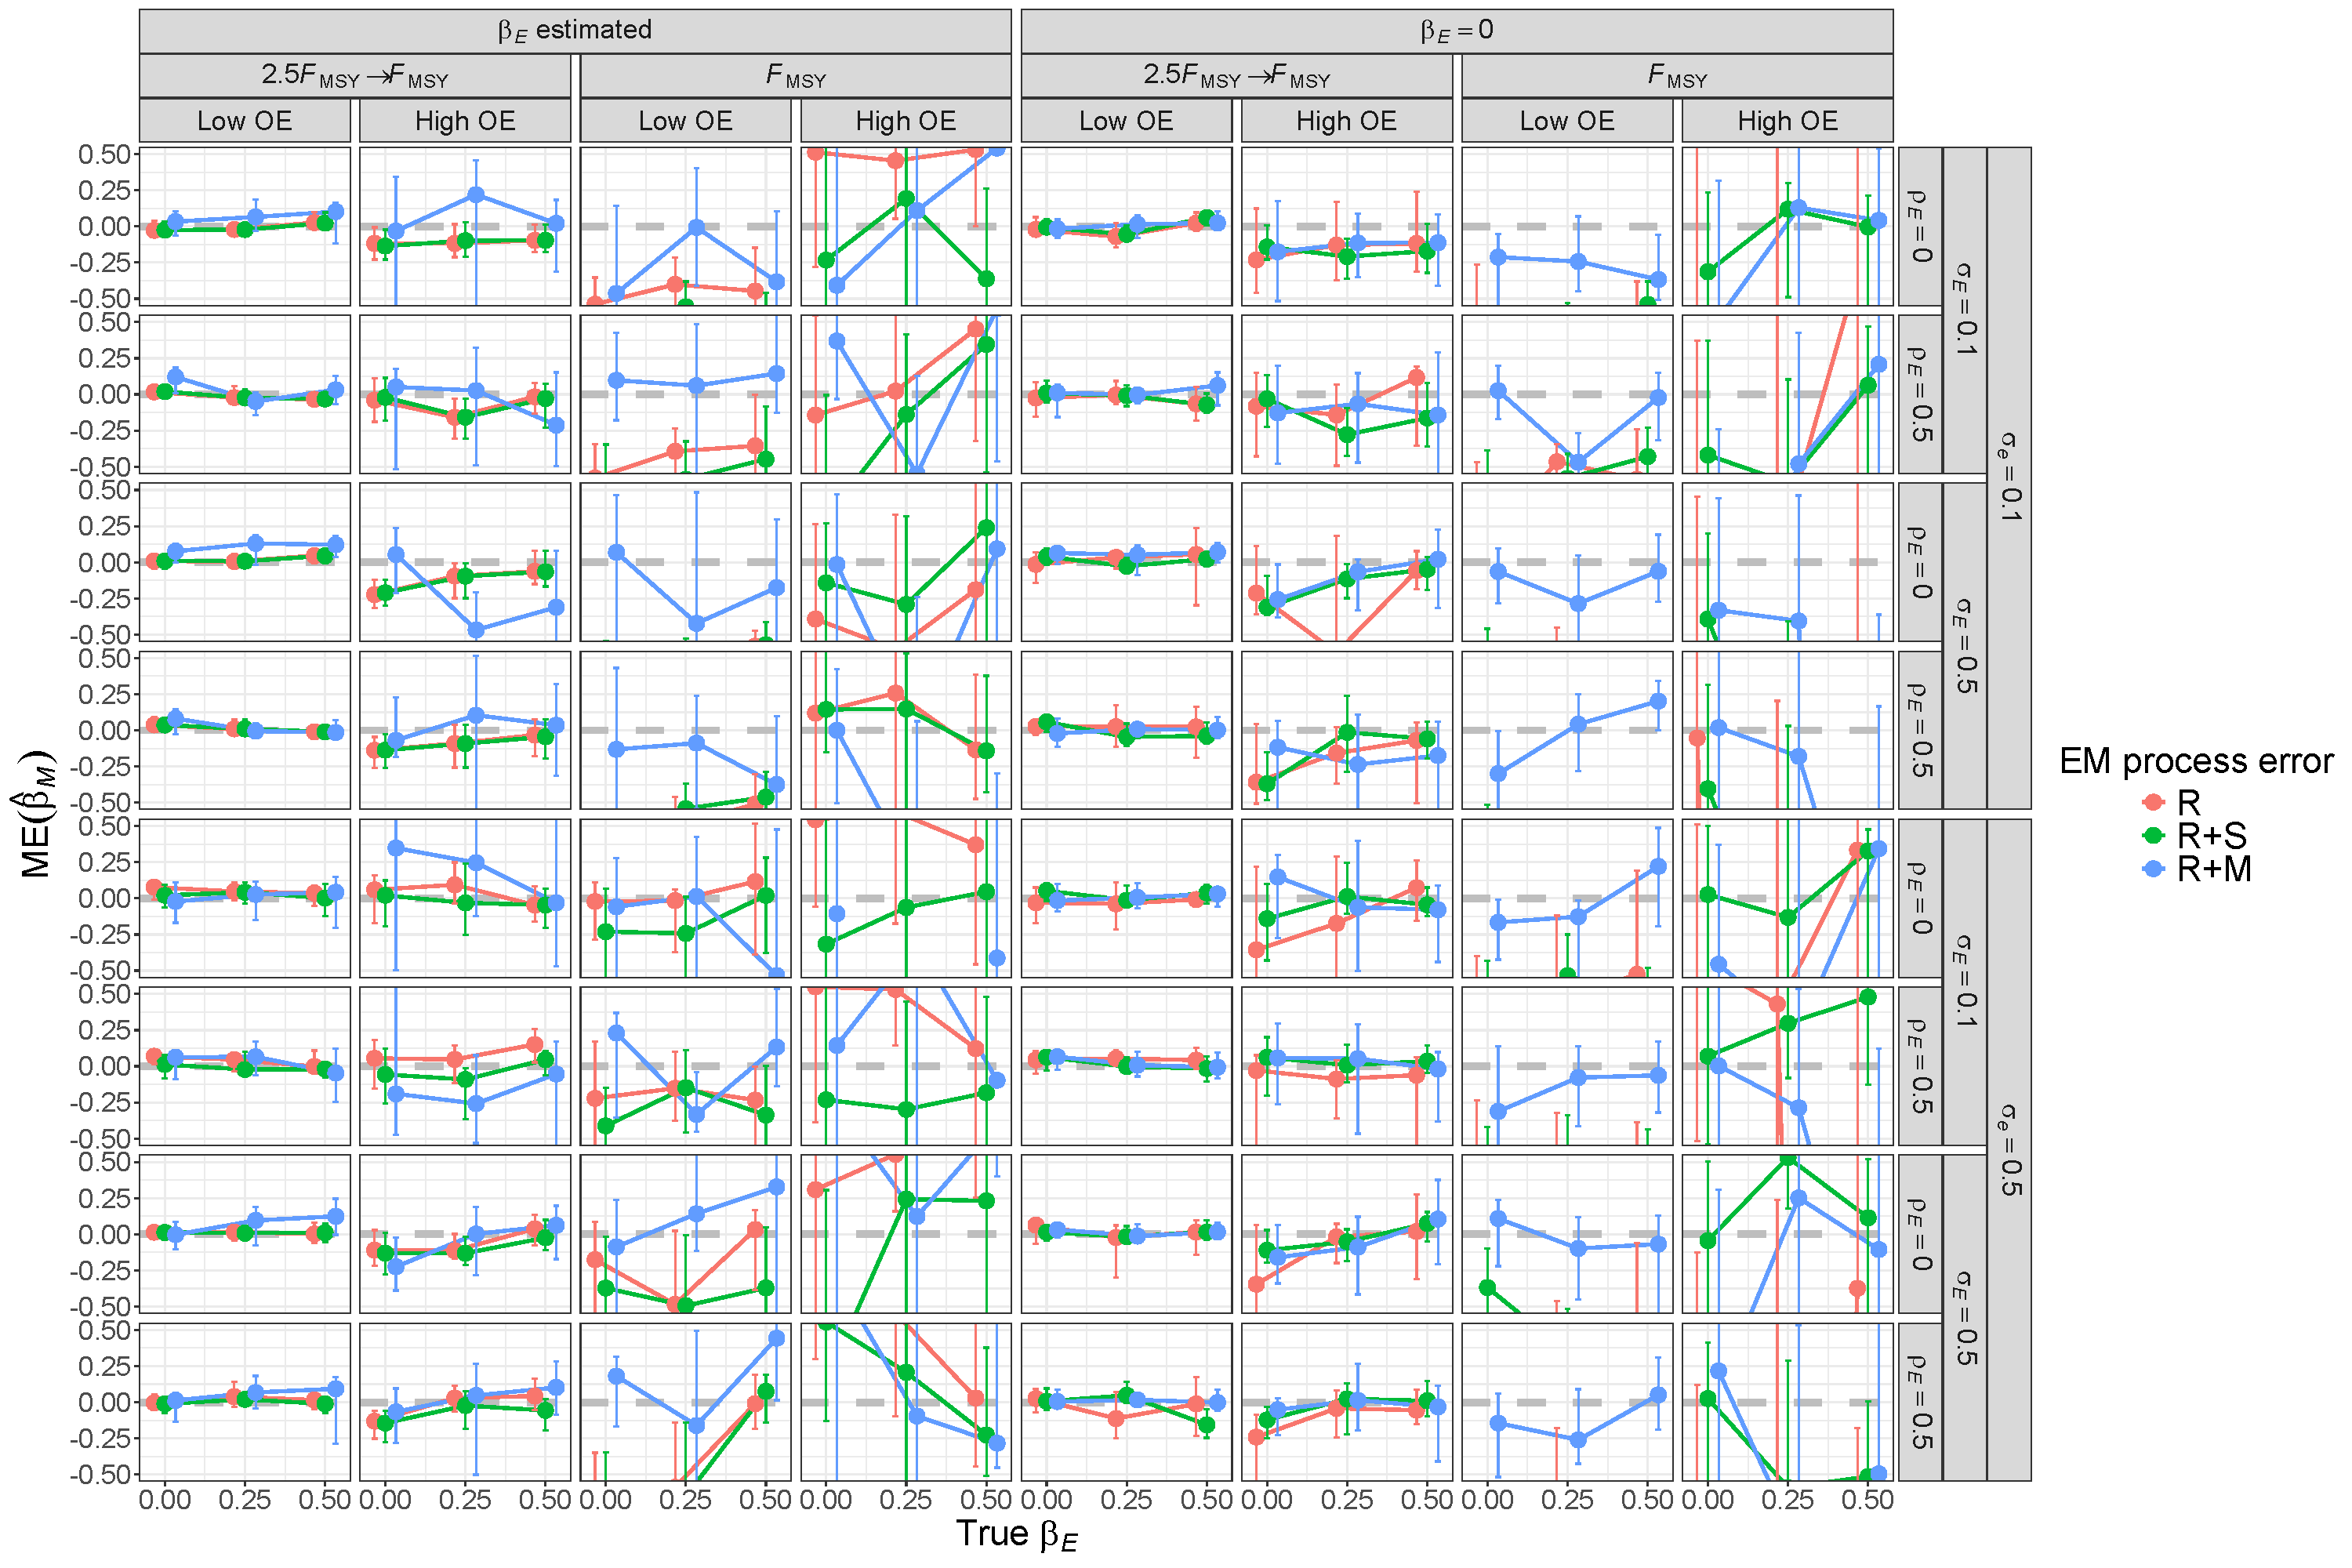
\includegraphics[height = \textheight]{beta_M_bias_RMom}
\end{center}
\caption{For R+M OMs, median error (ME) of estimates of $\beta_M$ from fitting EMs with alternative process error assumptions and treatment of covariate effect ($\beta_E = 0$ or estimated). Vertical lines represent 95\% confidence intervals.}\label{beta_M_bias_RMom}
\end{figure}
\end{landscape}

\hypertarget{median-natural-mortality-parameter-standard-error-estimation-bias}{%
\subsection*{Median natural mortality parameter standard error estimation bias}\label{median-natural-mortality-parameter-standard-error-estimation-bias}}
\addcontentsline{toc}{subsection}{Median natural mortality parameter standard error estimation bias}

\begin{landscape}
\begin{figure}
\begin{center}
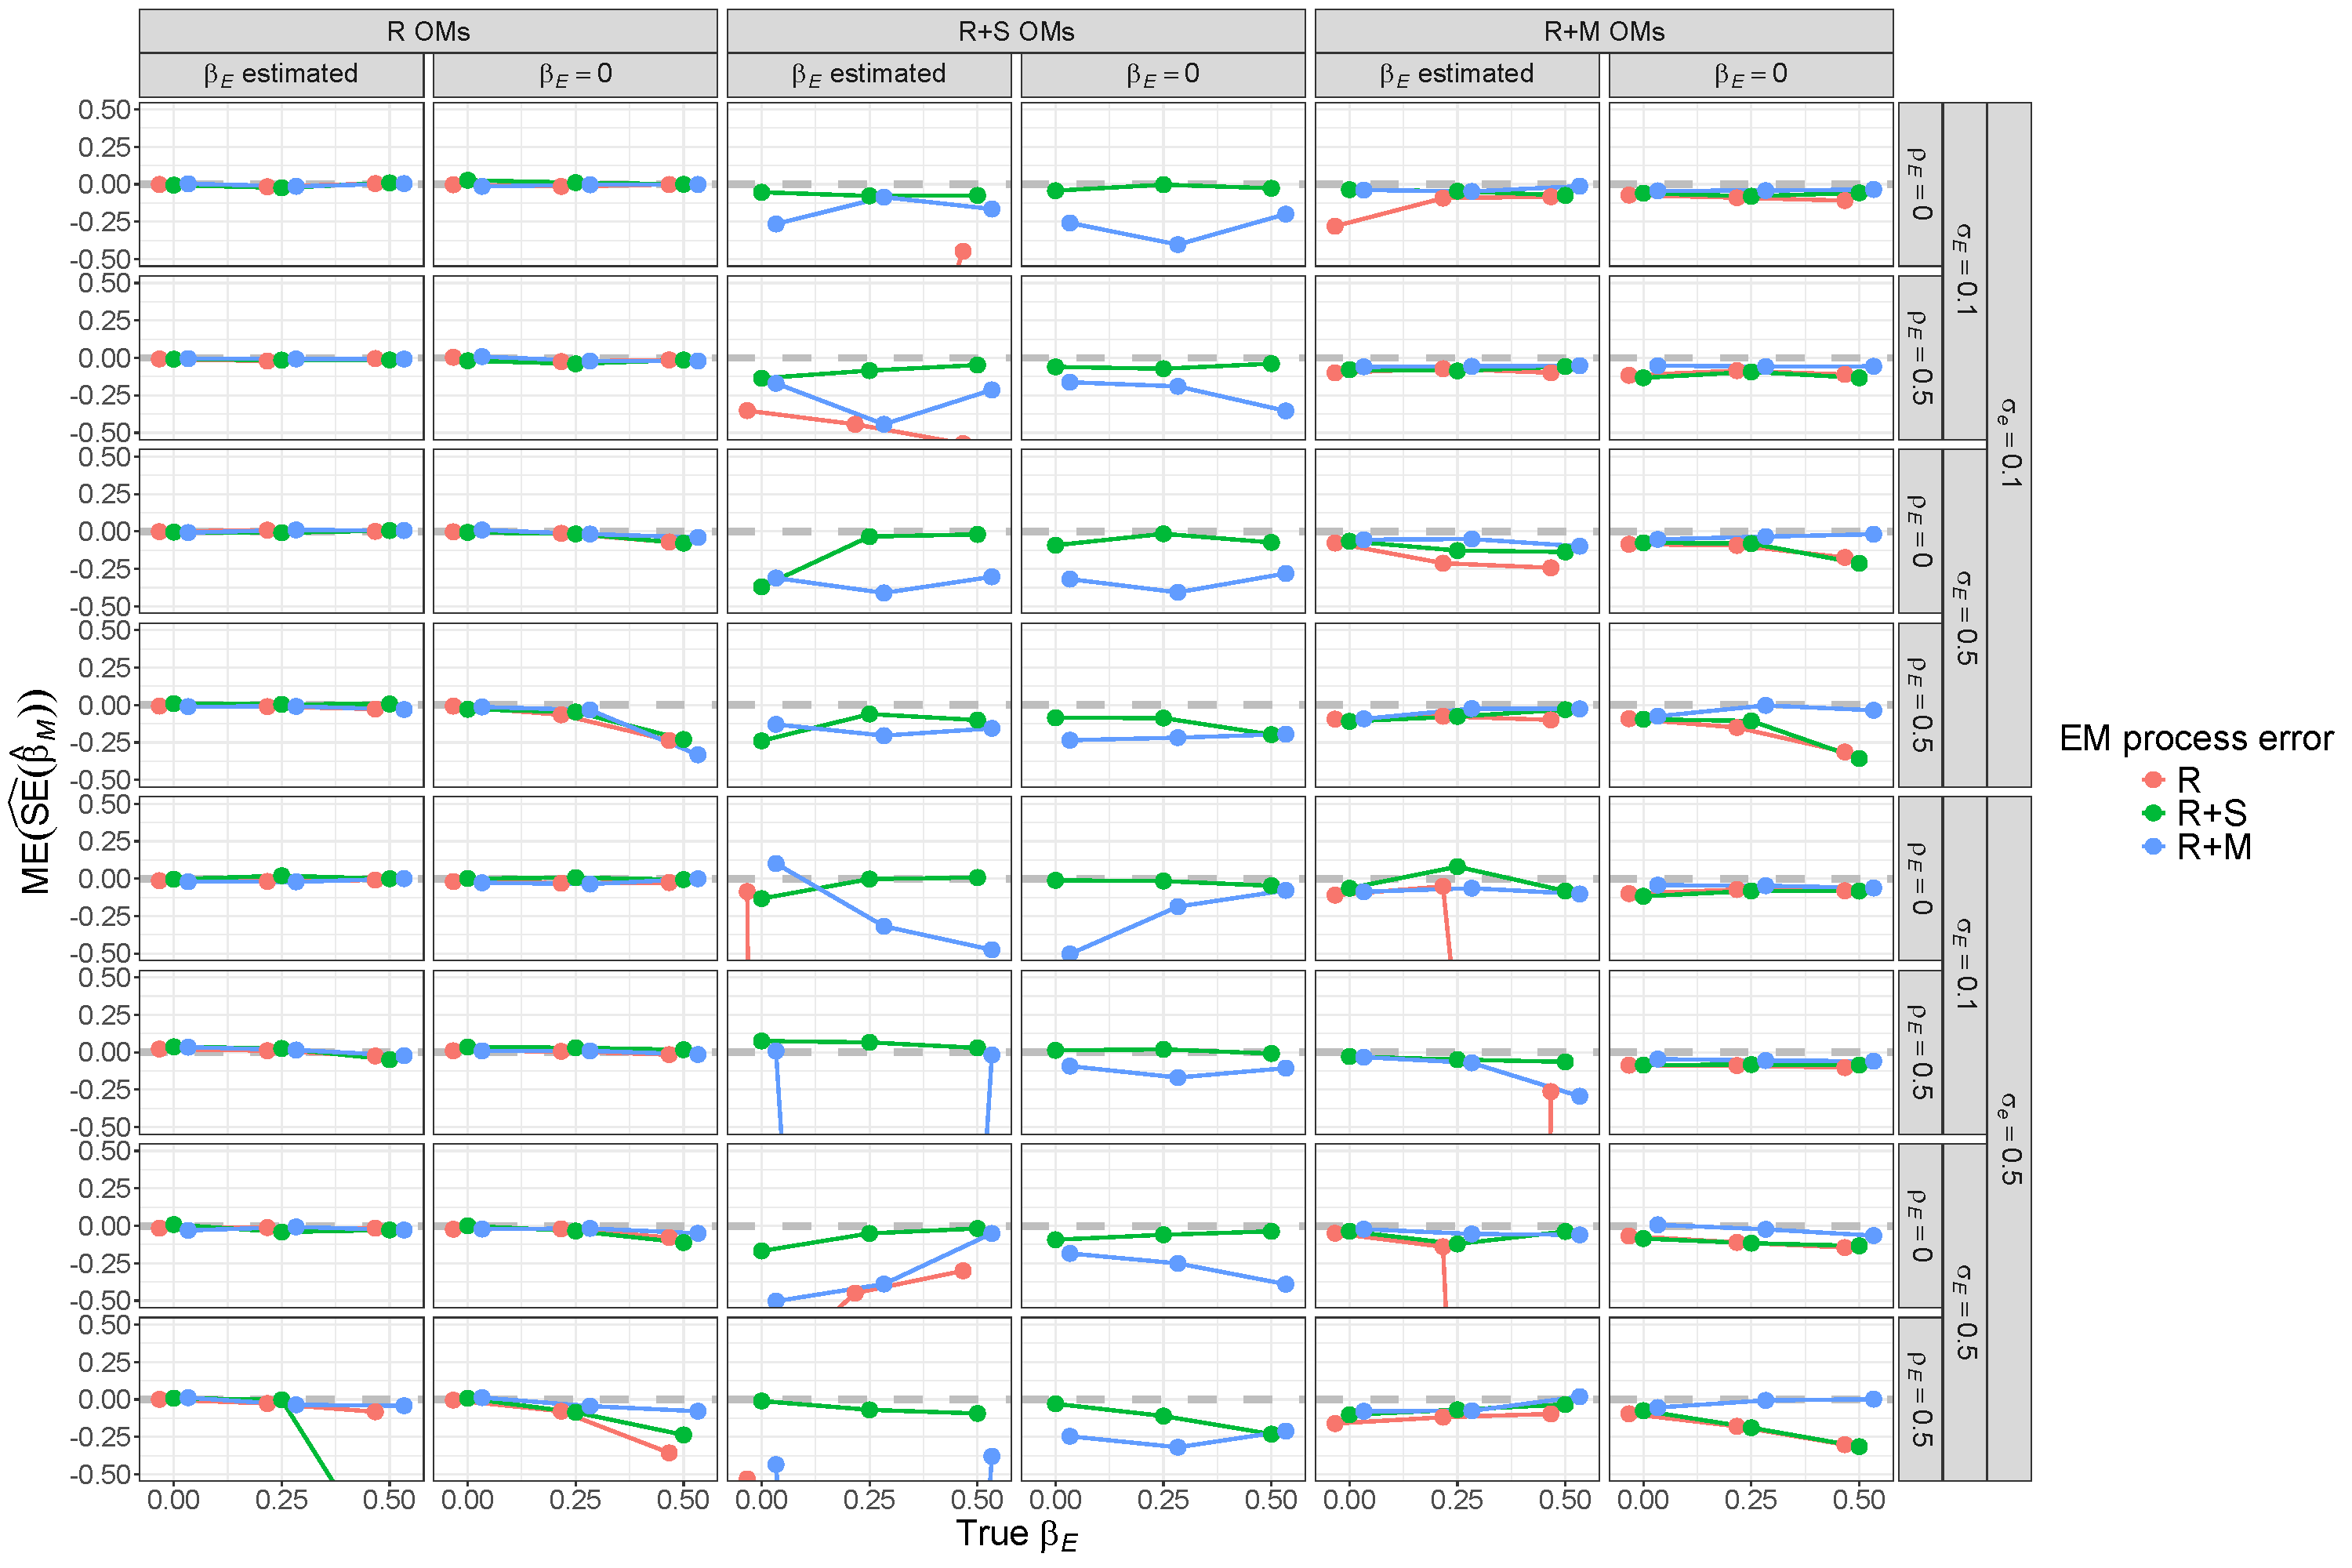
\includegraphics[height = \textheight]{se_beta_M_bias_main}
\end{center}
\caption{Median error (ME) of Hessian-based estimates of standard error for median natural mortality parameter $\beta_M$ from fitting EMs with alternative process error assumptions and treatment of the covariate effect ($\beta_ E= 0$ or estimated). All OMs had low observation error and contrast in fishing mortality. True standard error is defined as the mean of the standard error estimates accross converged fits to simulated data sets for a given OM scenario.}\label{se_beta_M_bias}
\end{figure}
\end{landscape}

\begin{landscape}
\begin{figure}
\begin{center}
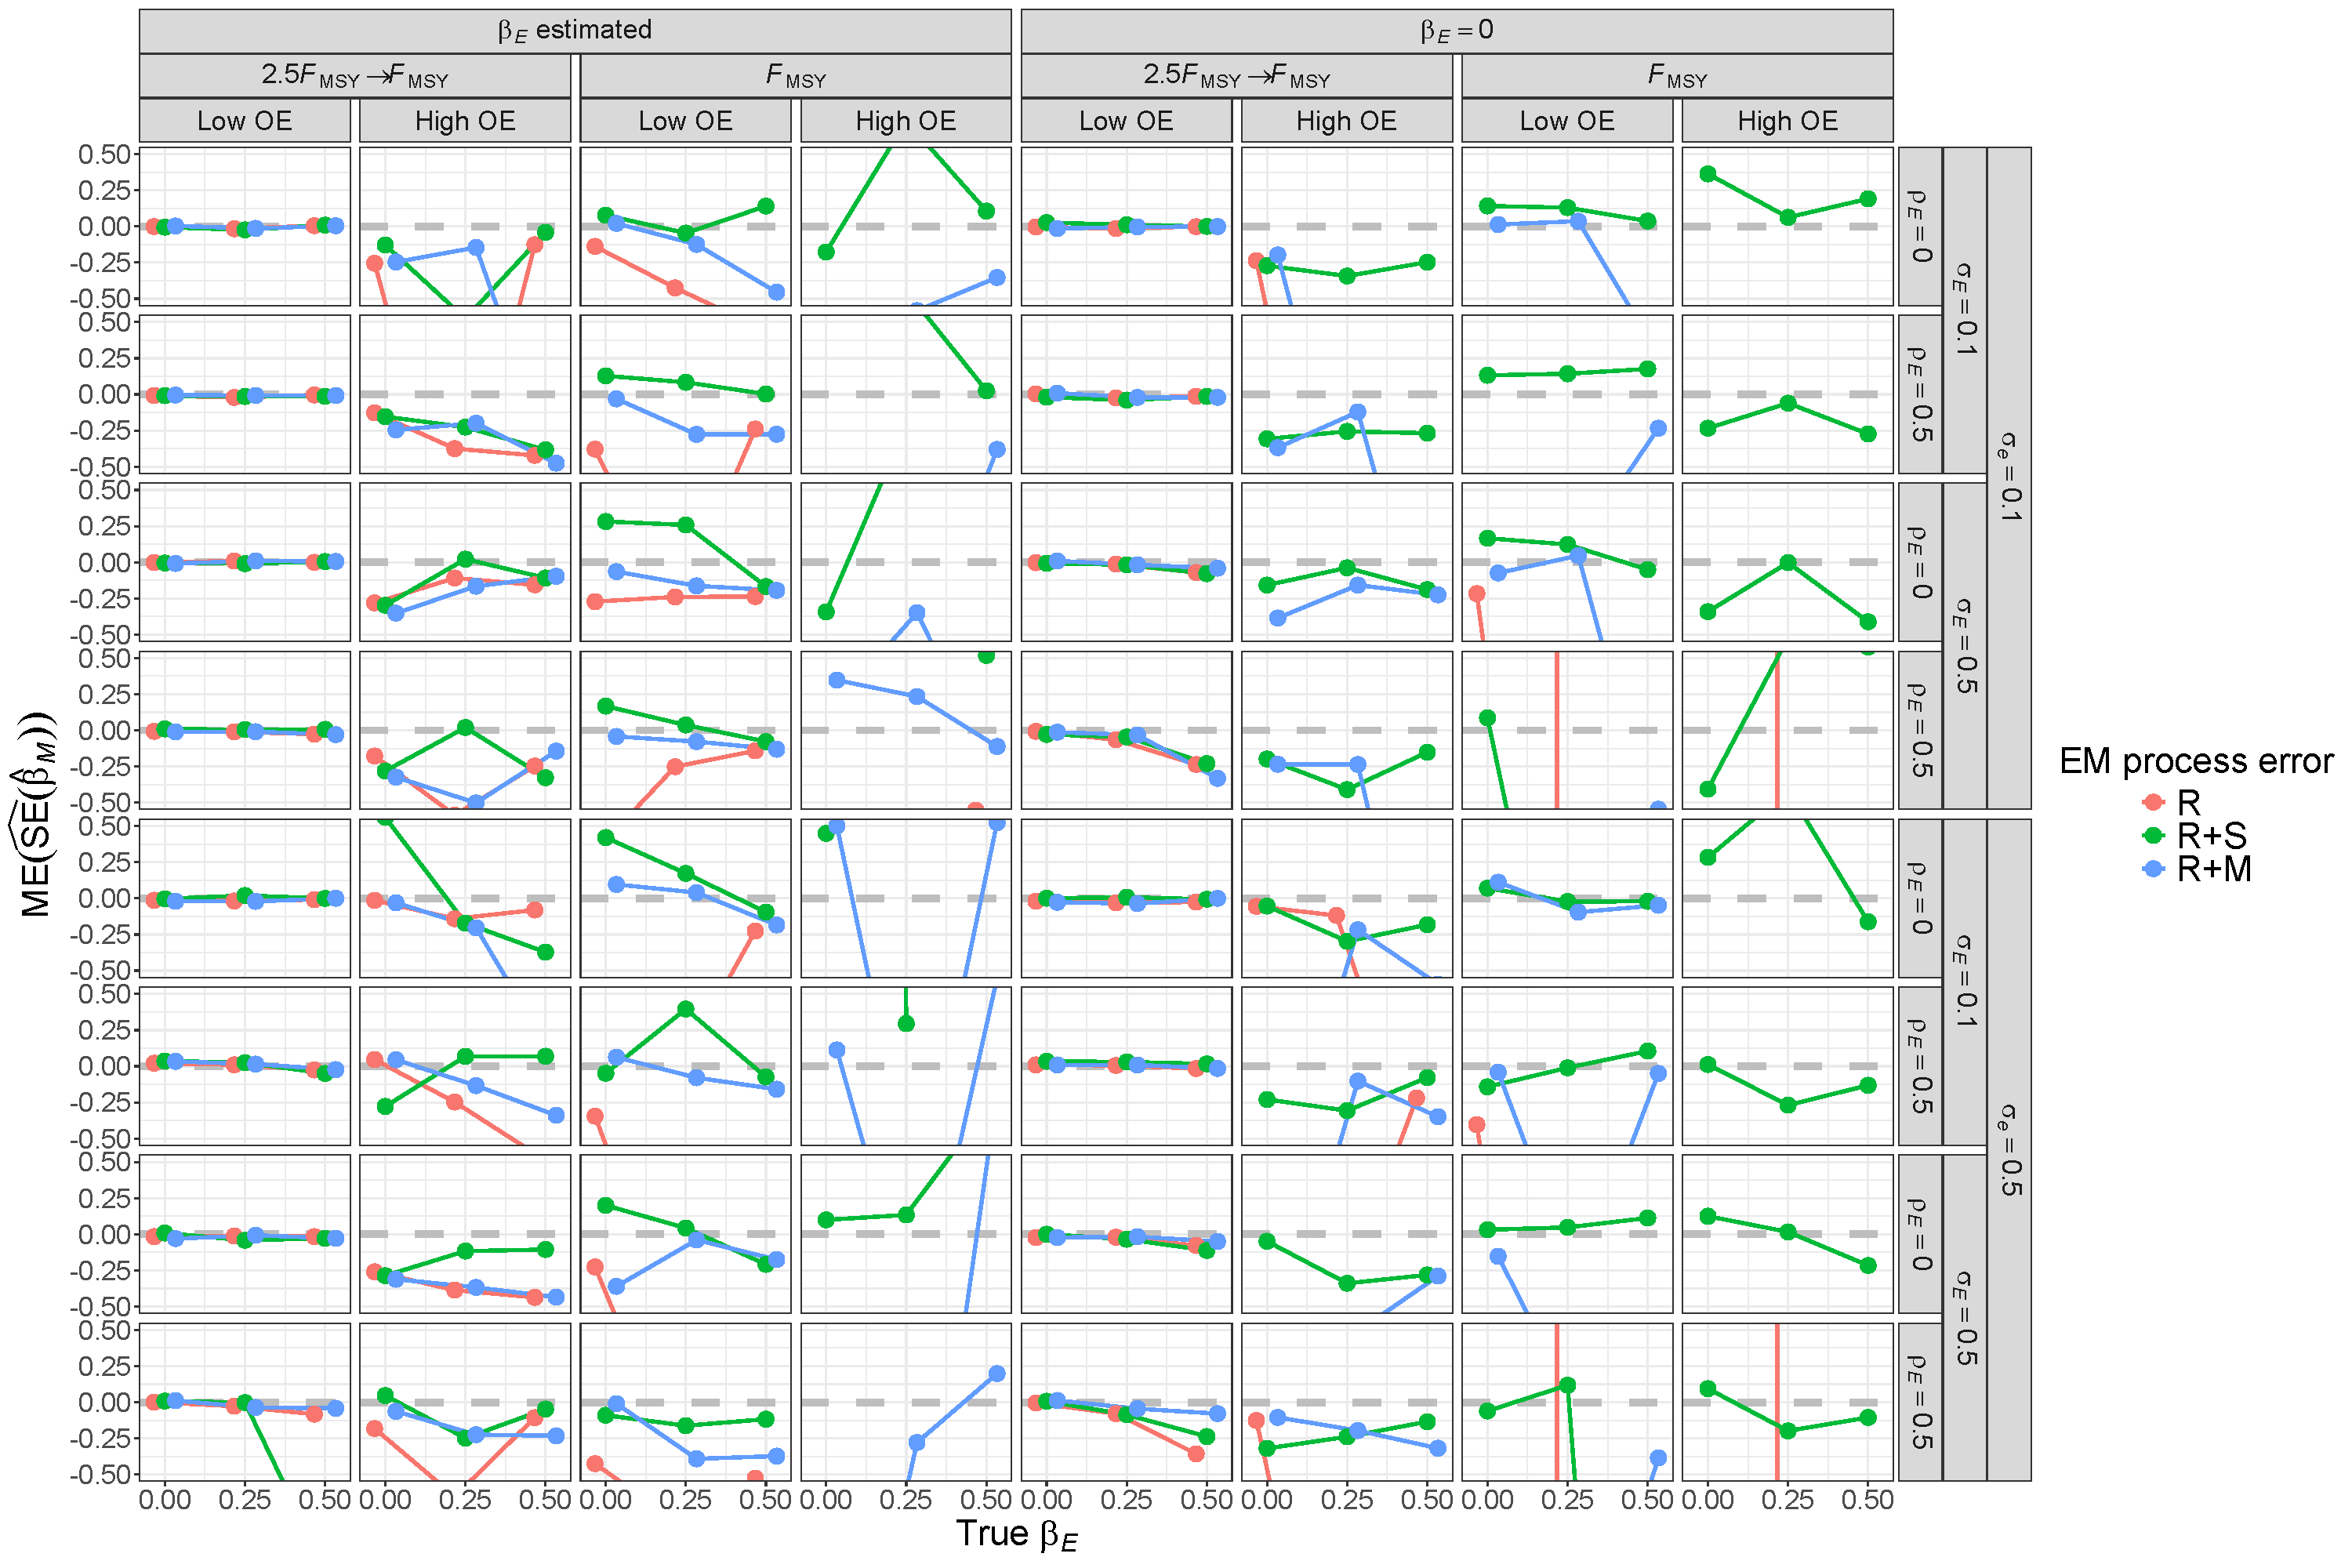
\includegraphics[height = \textheight]{se_beta_M_bias_Rom}
\end{center}
\caption{For R OMs, median error (ME) of Hessian-based estimates of standard error for median natural mortality parameter $\beta_M$ from fitting EMs with alternative process error assumptions and treatment of the covariate effect ($\beta_ E= 0$ or estimated). True standard error is defined as the mean of the standard error estimates accross converged fits to simulated data sets for a given OM scenario.}\label{se_beta_M_bias_Rom}
\end{figure}
\end{landscape}

\begin{landscape}
\begin{figure}
\begin{center}
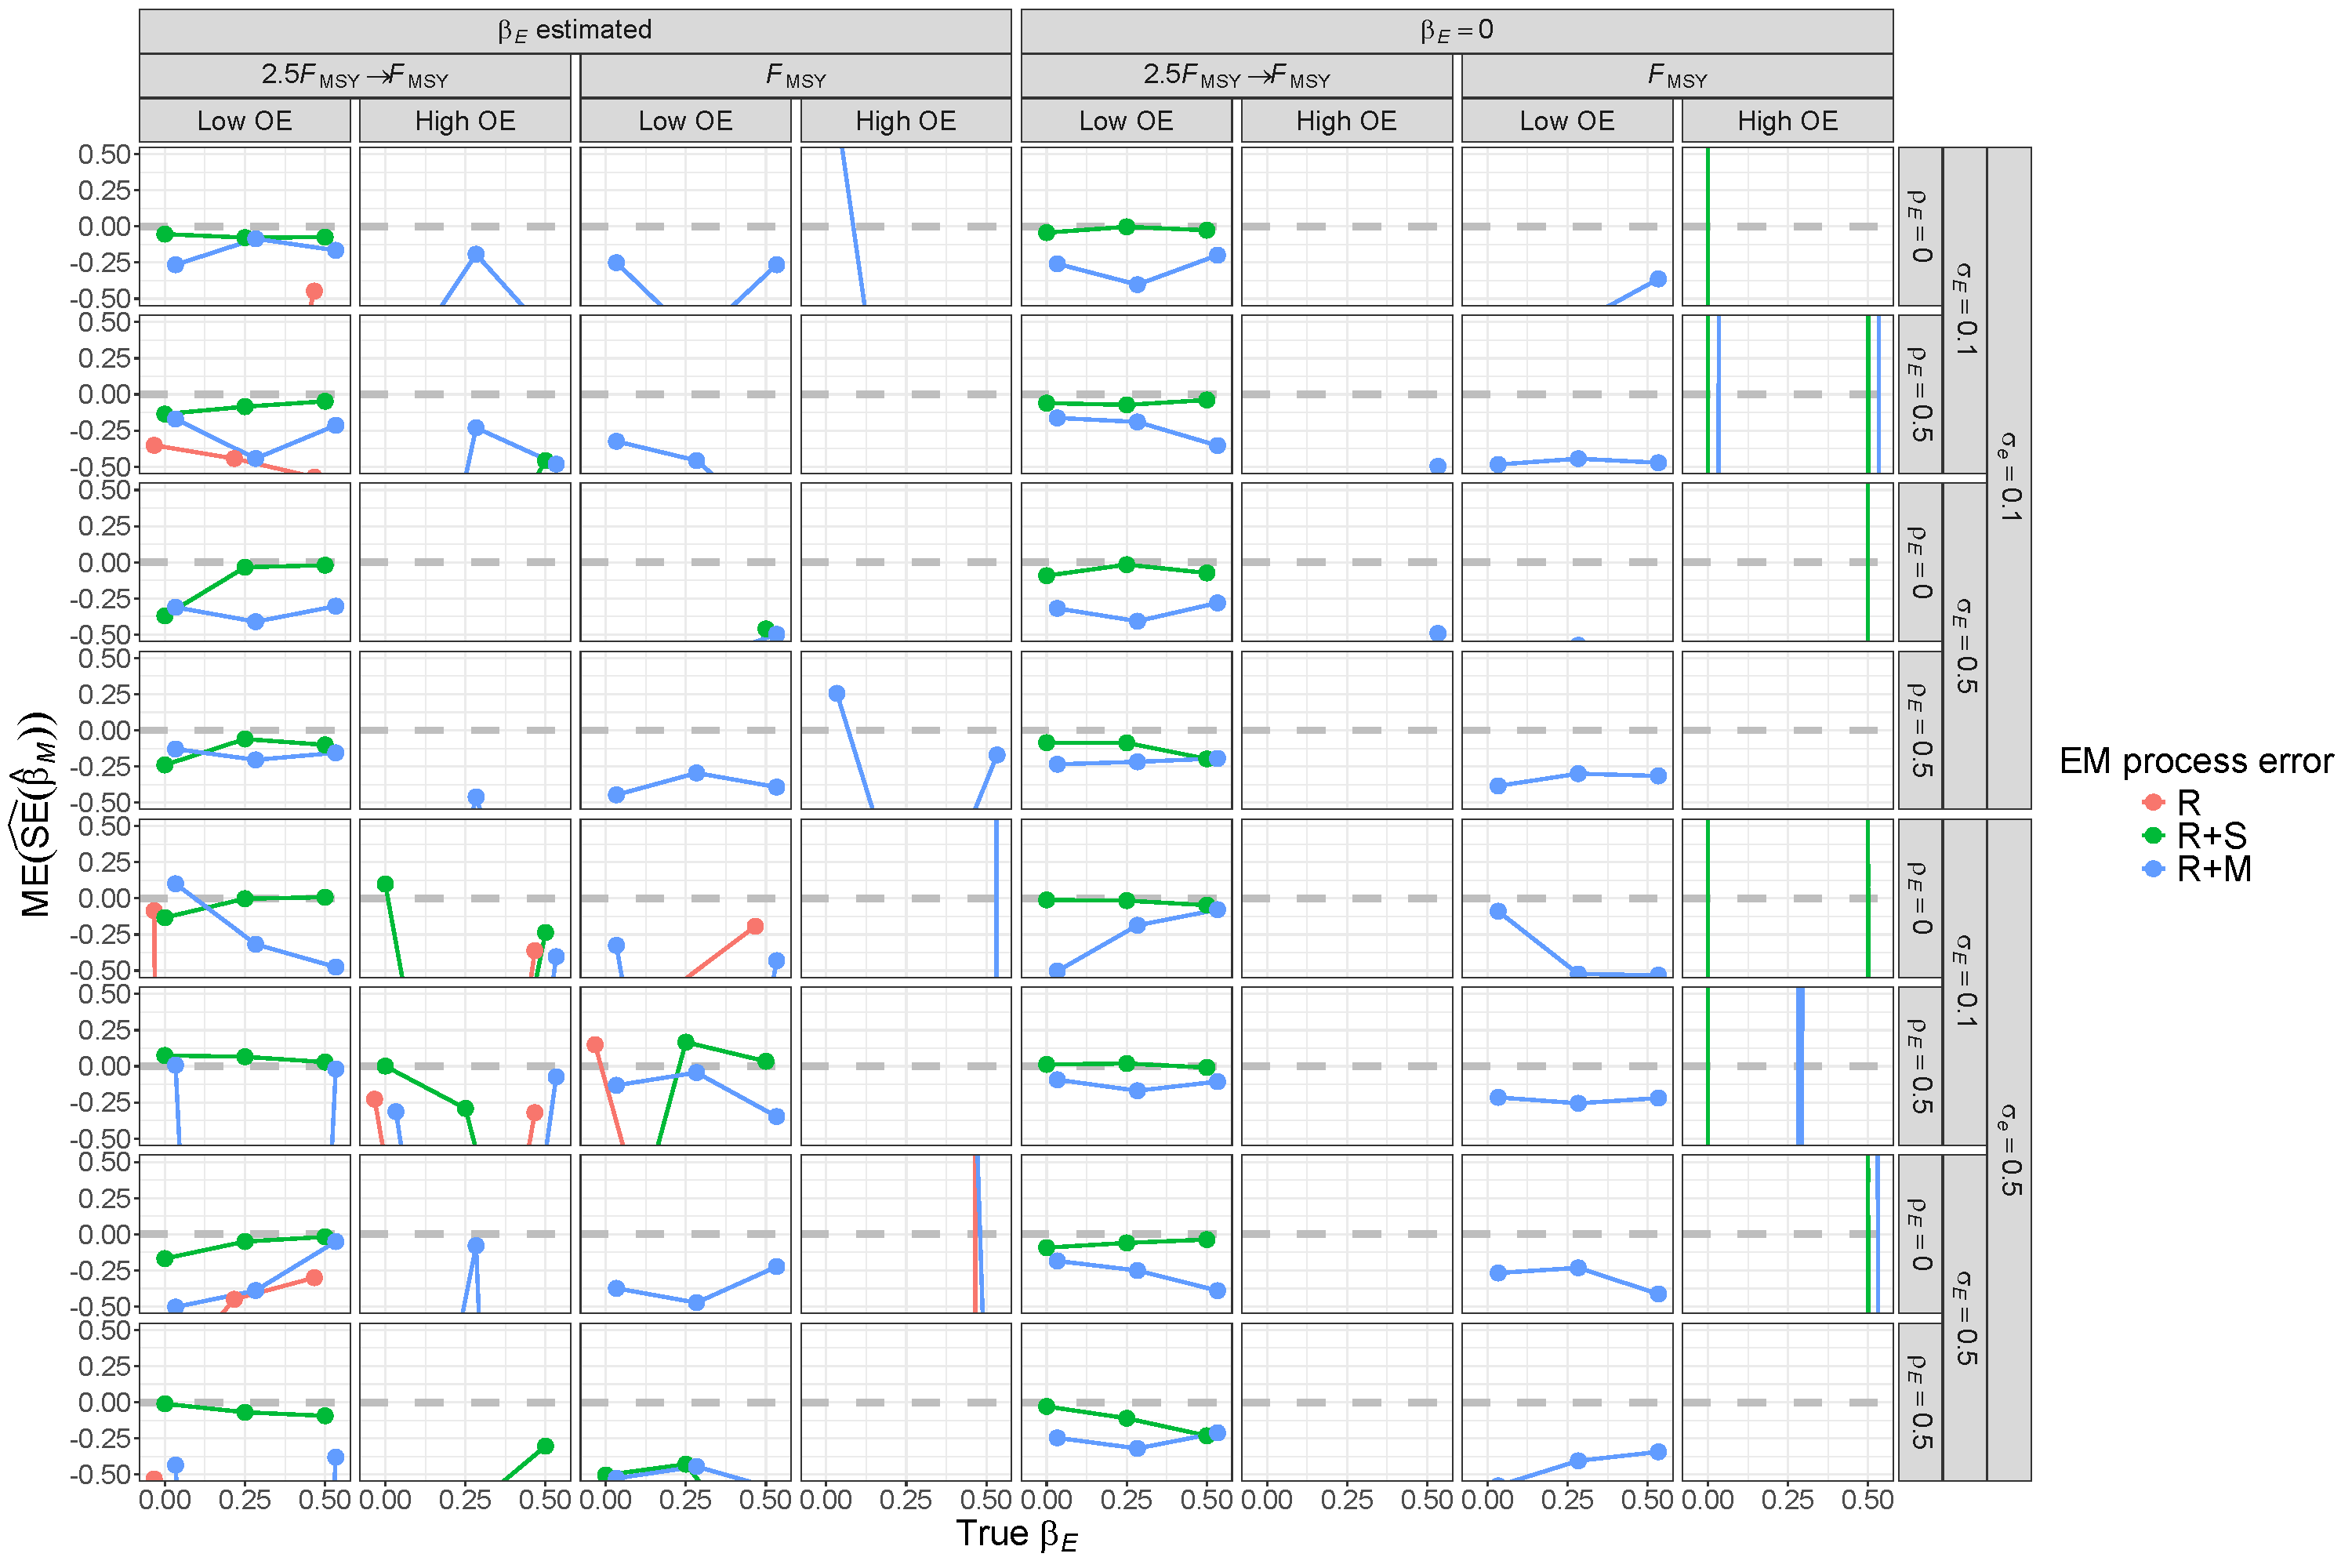
\includegraphics[height = \textheight]{se_beta_M_bias_RSom}
\end{center}
\caption{For R+S OMs, median error (ME) of Hessian-based estimates of standard error for median natural mortality parameter $\beta_M$ from fitting EMs with alternative process error assumptions and treatment of the covariate effect ($\beta_ E= 0$ or estimated). True standard error is defined as the mean of the standard error estimates accross converged fits to simulated data sets for a given OM scenario.}\label{se_beta_M_bias_RSom}
\end{figure}
\end{landscape}

\begin{landscape}
\begin{figure}
\begin{center}
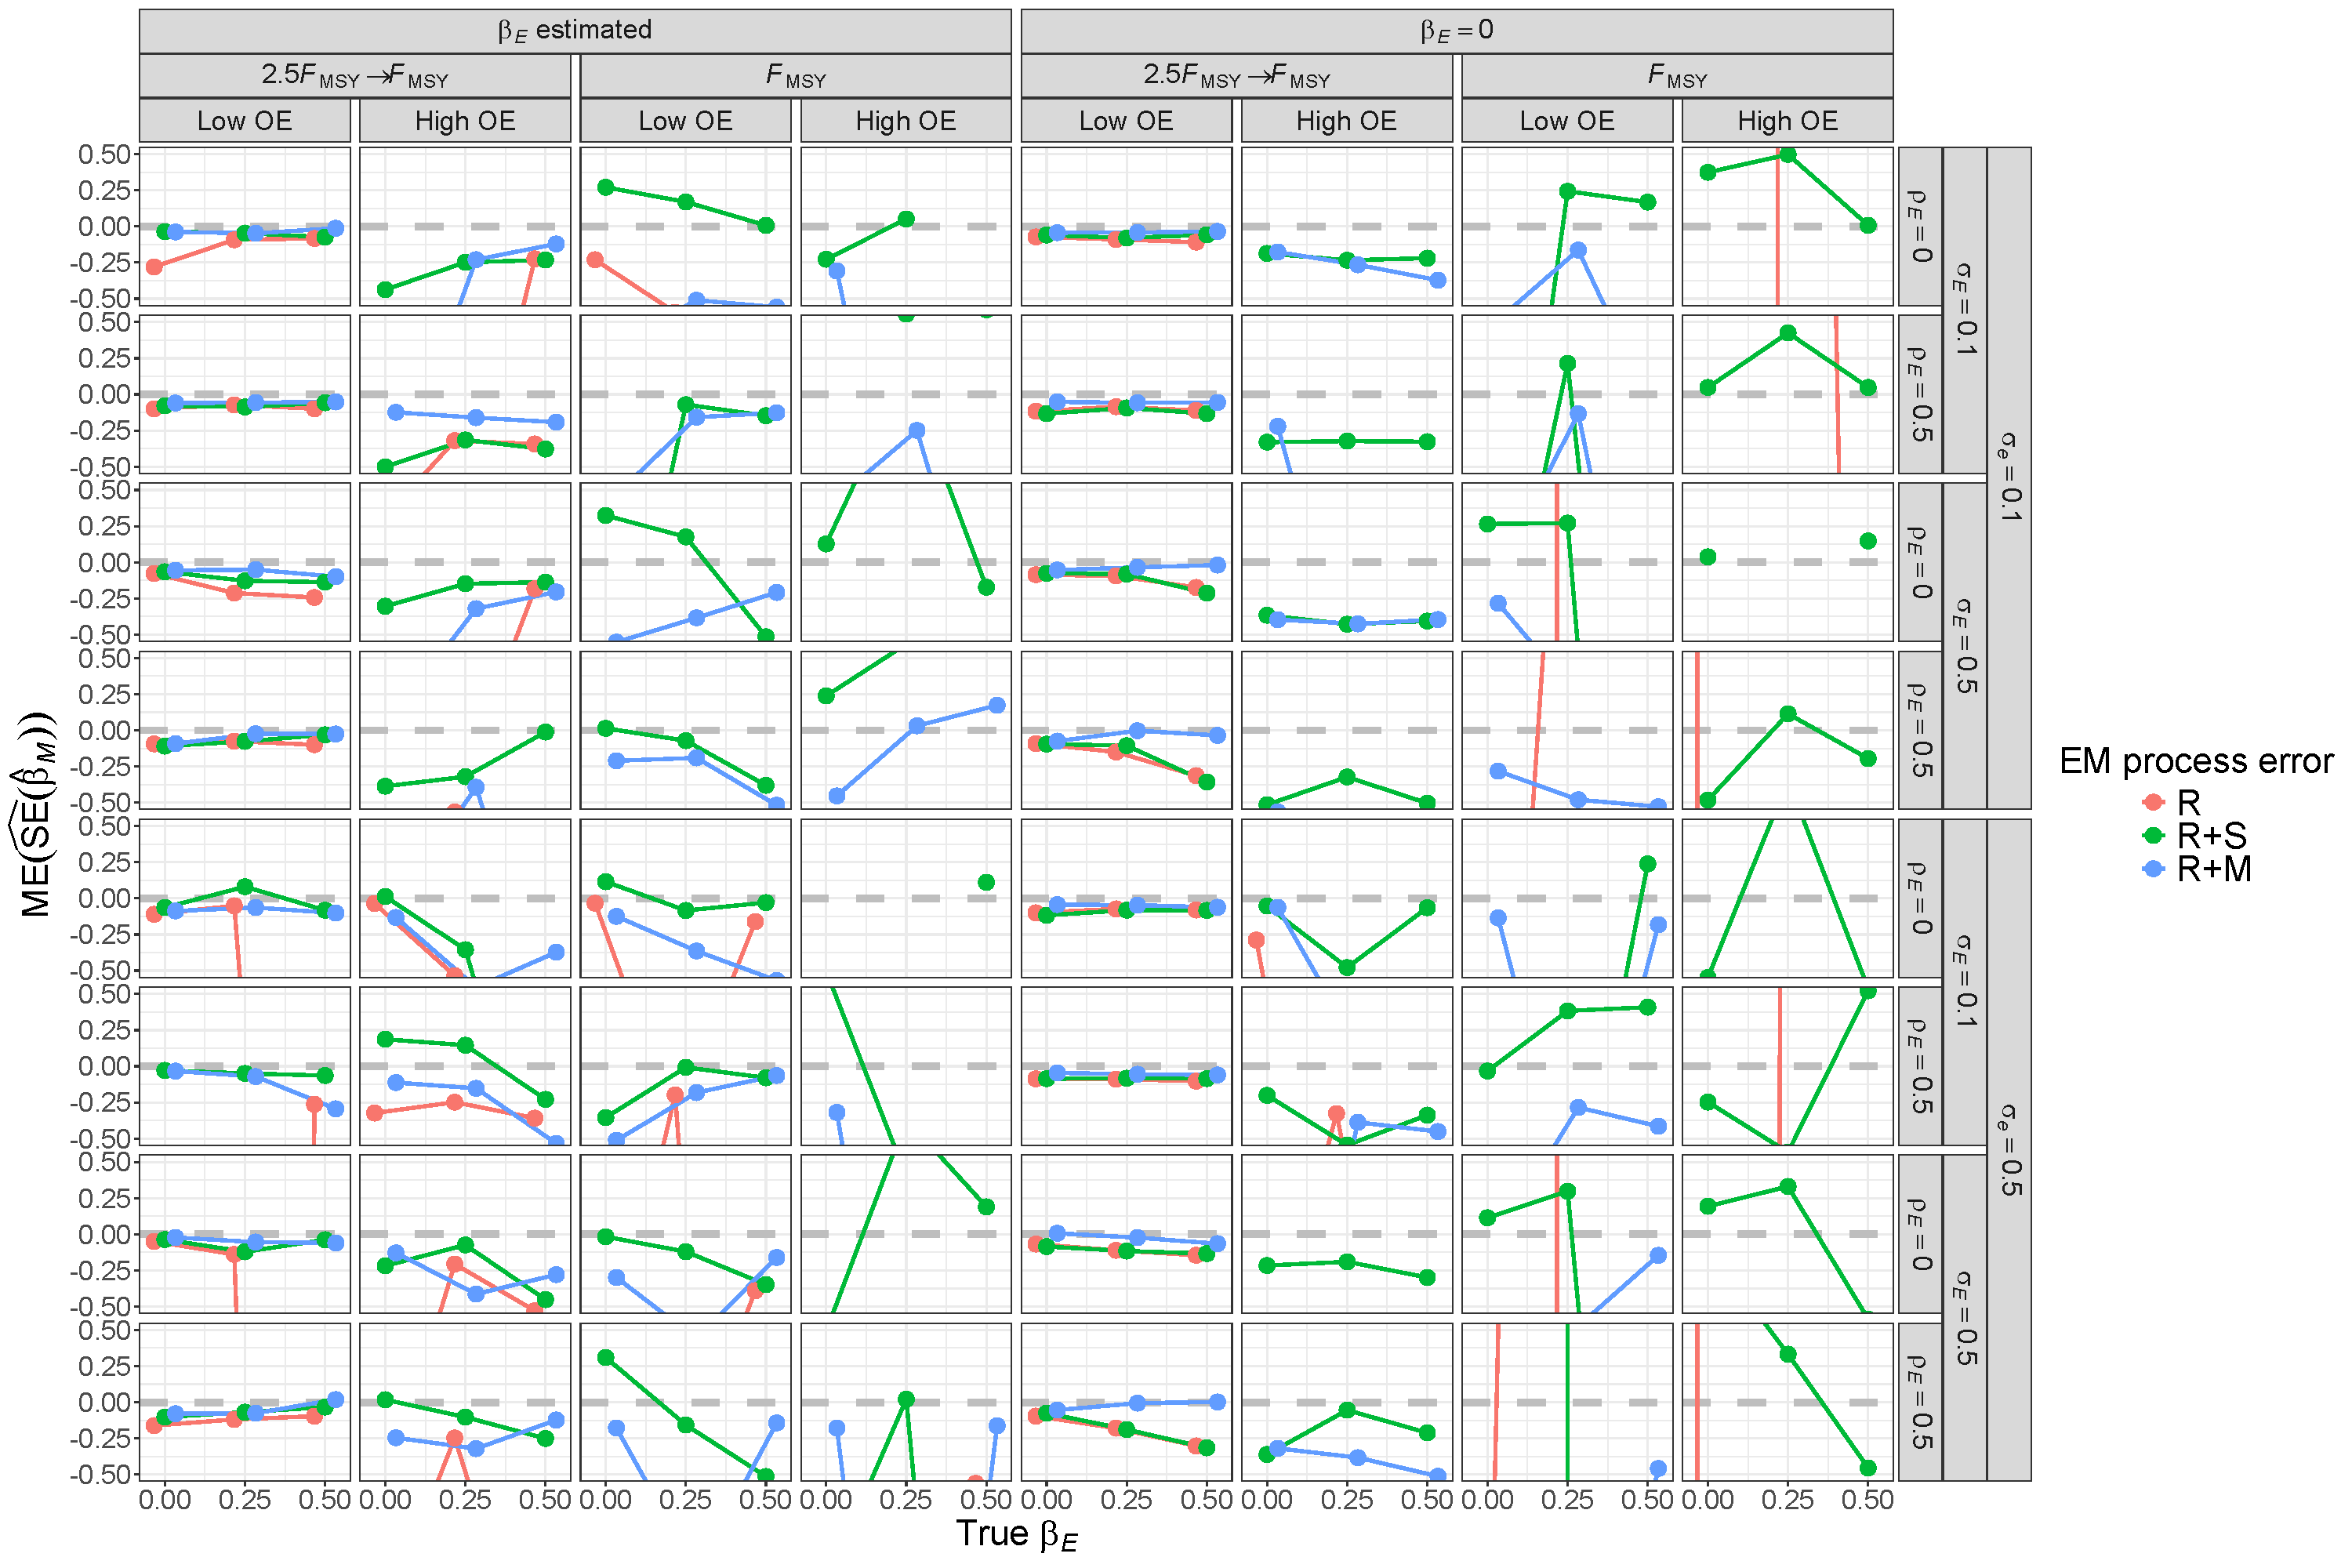
\includegraphics[height = \textheight]{se_beta_M_bias_RMom}
\end{center}
\caption{For R+M OMs, median error (ME) of Hessian-based estimates of standard error for median natural mortality parameter $\beta_M$ from fitting EMs with alternative process error assumptions and treatment of the covariate effect ($\beta_ E= 0$ or estimated). True standard error is defined as the mean of the standard error estimates accross converged fits to simulated data sets for a given OM scenario.}\label{se_beta_M_bias_RMom}
\end{figure}
\end{landscape}

\hypertarget{median-natural-mortality-parameter-confidence-interval-coverage}{%
\subsection*{Median Natural mortality parameter confidence interval coverage}\label{median-natural-mortality-parameter-confidence-interval-coverage}}
\addcontentsline{toc}{subsection}{Median Natural mortality parameter confidence interval coverage}

\begin{landscape}
\begin{figure}
\begin{center}
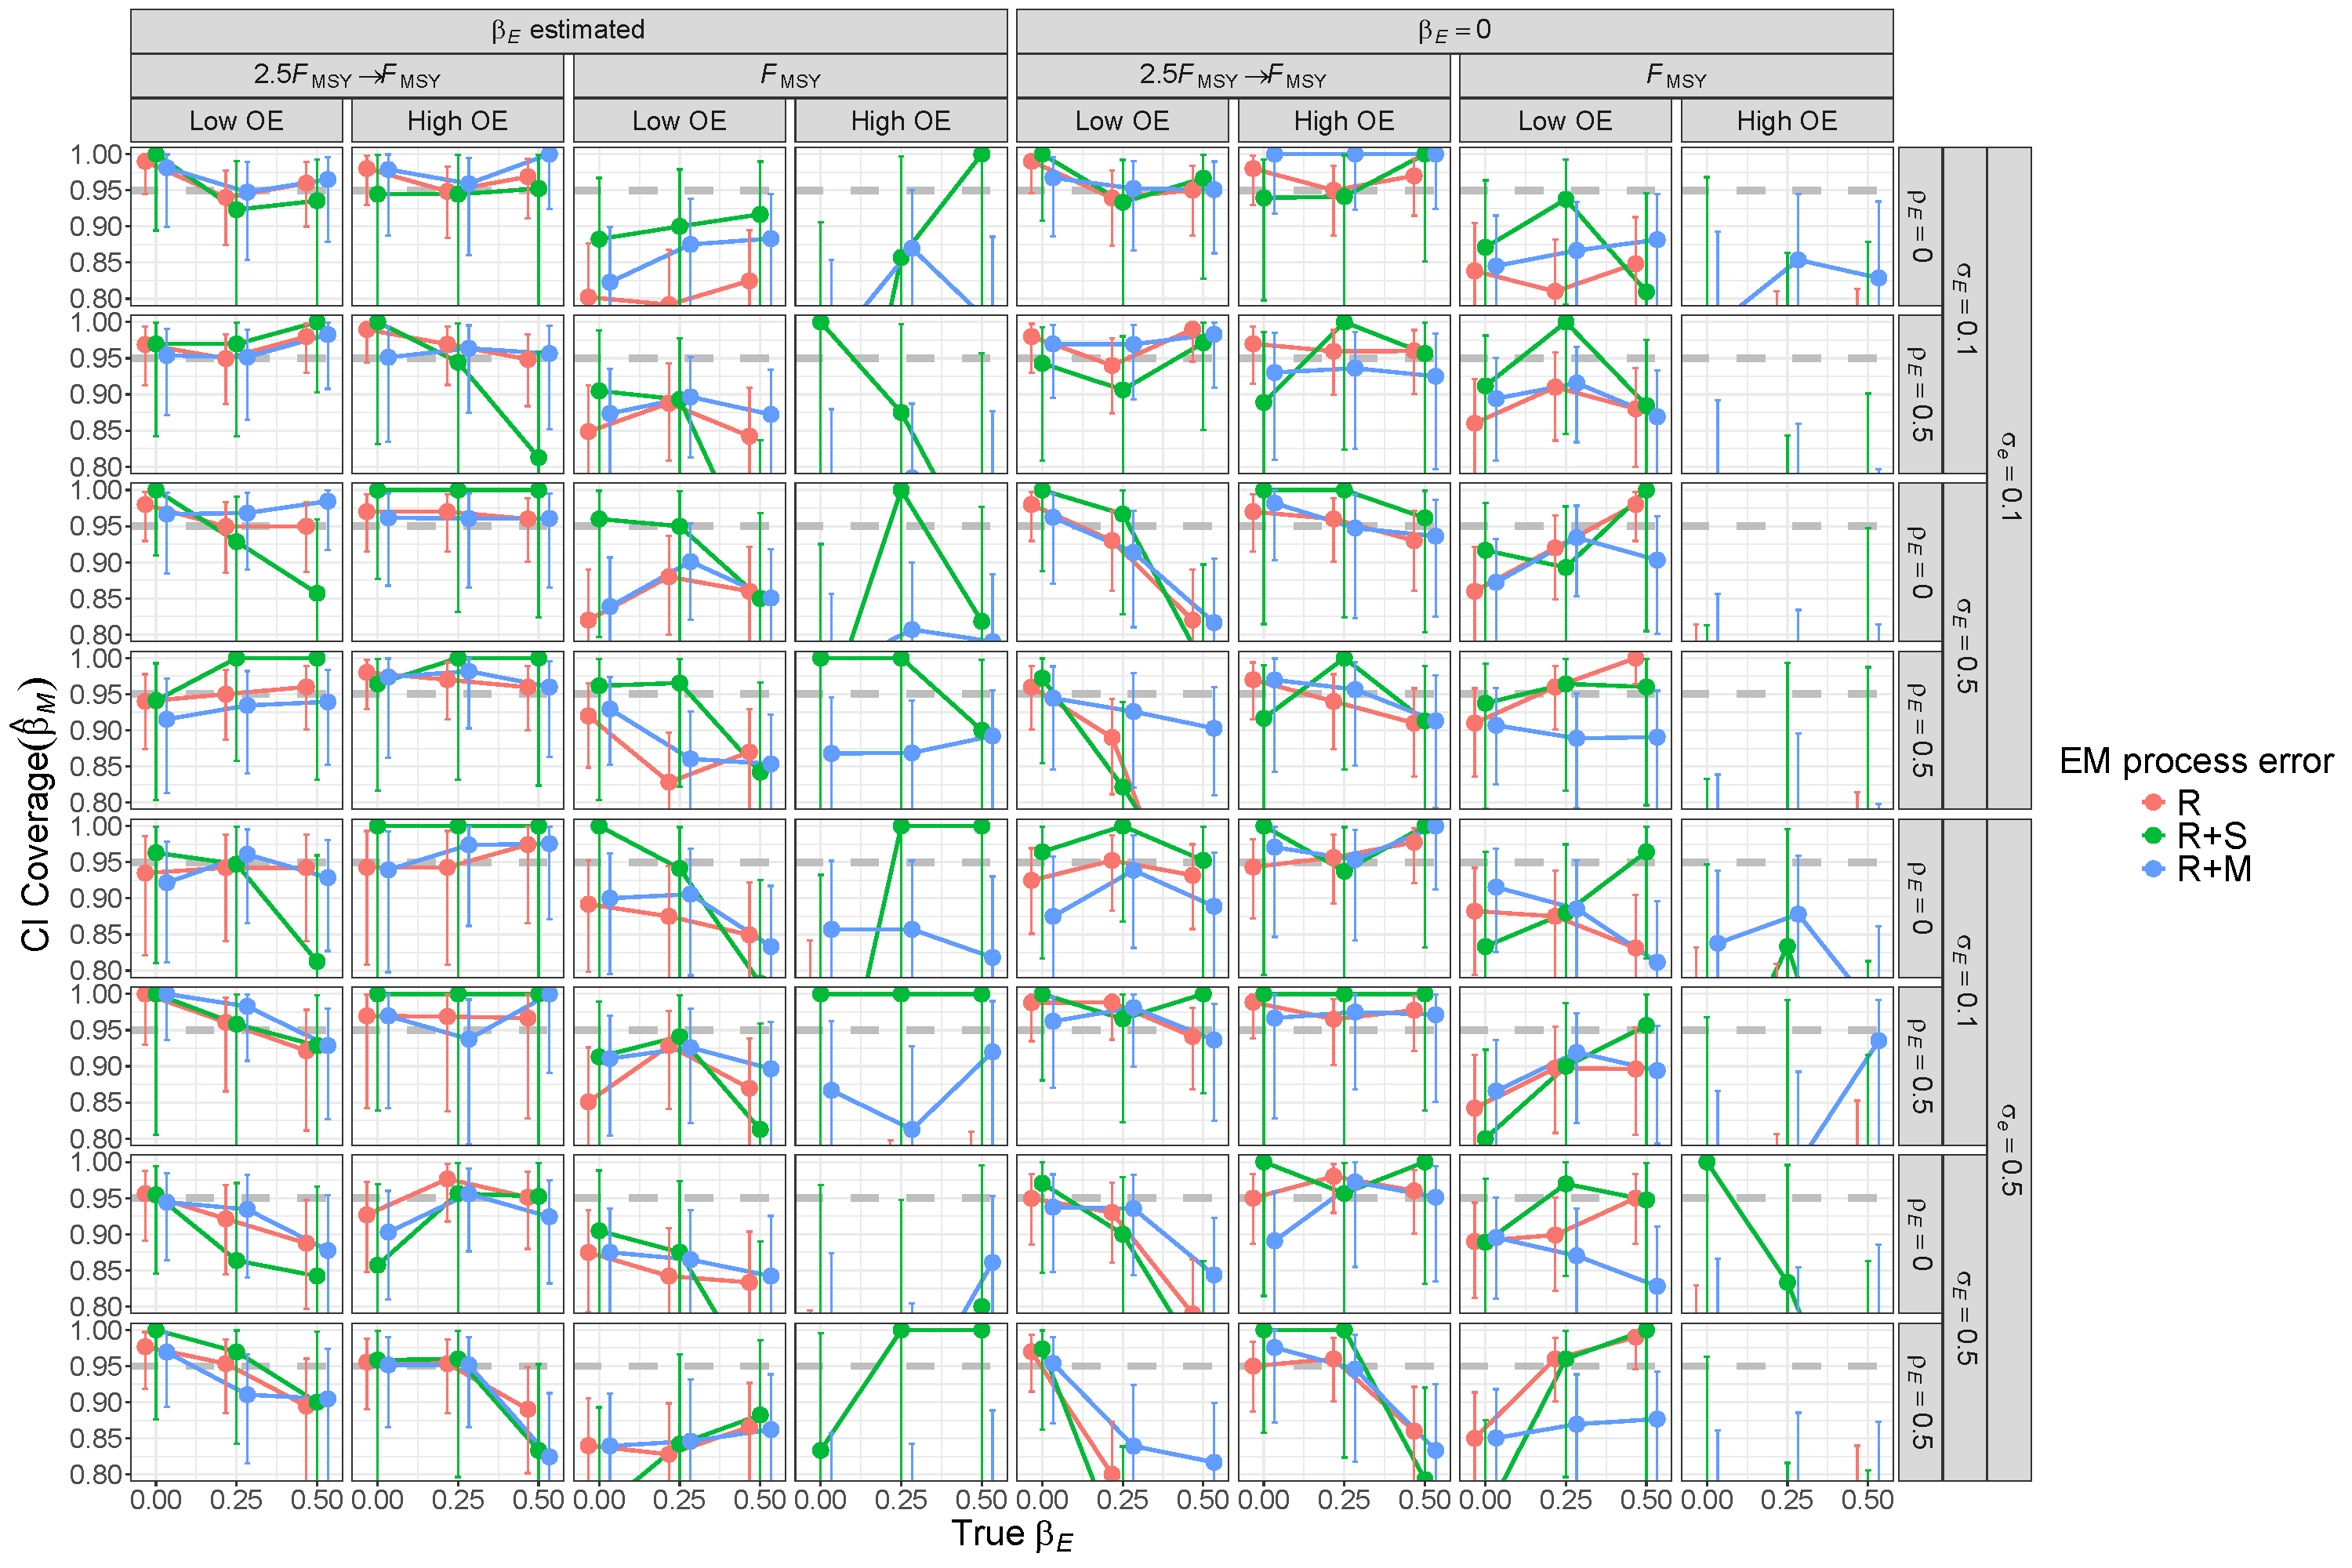
\includegraphics[height = \textheight]{beta_M_CI_coverage_Rom}
\end{center}
\caption{For R OMs, probability of 95\% confidence interval for $\beta_M$ containing the true value for EMs with alternative process error assumptions and treatment of covariate effect ($\beta_E = 0$ or estimated). Vertical lines represent 95\% confidence intervals.}\label{beta_M_CI_coverage_Rom}
\end{figure}
\end{landscape}

\begin{landscape}
\begin{figure}
\begin{center}
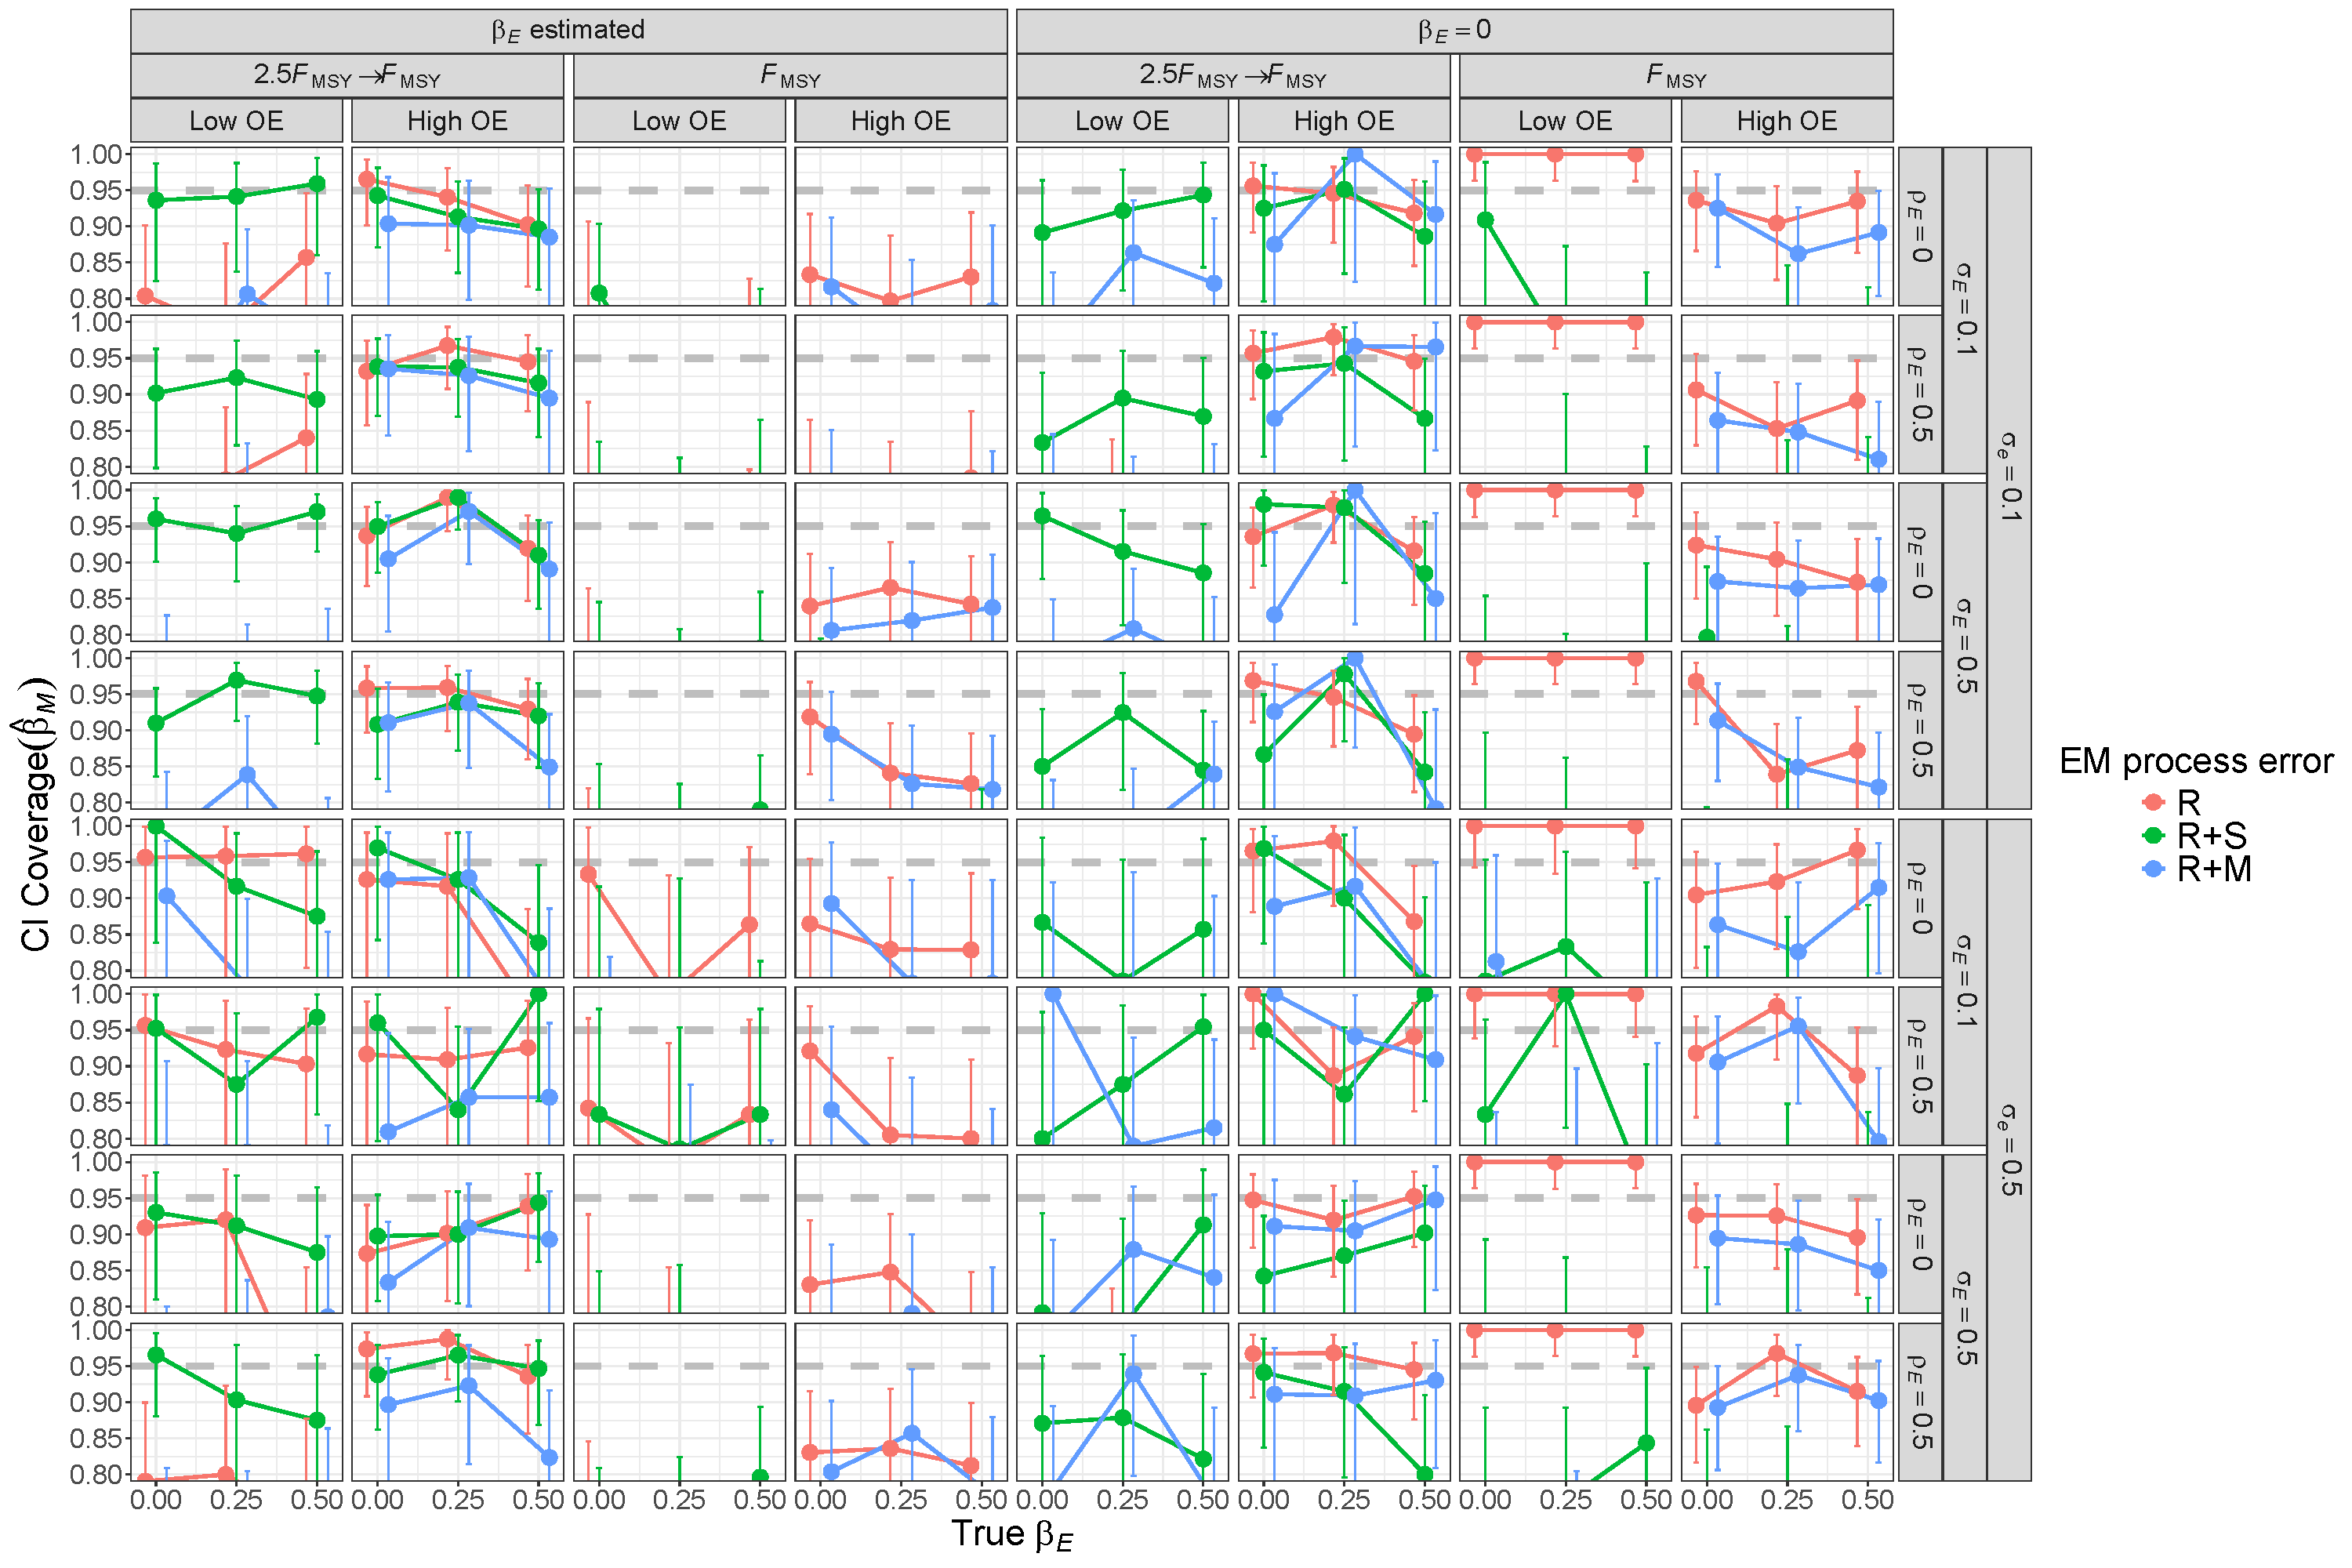
\includegraphics[height = \textheight]{beta_M_CI_coverage_RSom}
\end{center}
\caption{For R+S OMs, probability of 95\% confidence interval for $\beta_M$ containing the true value for EMs with alternative process error assumptions and treatment of covariate effect ($\beta_E = 0$ or estimated). Vertical lines represent 95\% confidence intervals.}\label{beta_M_CI_coverage_RSom}
\end{figure}
\end{landscape}

\begin{landscape}
\begin{figure}
\begin{center}
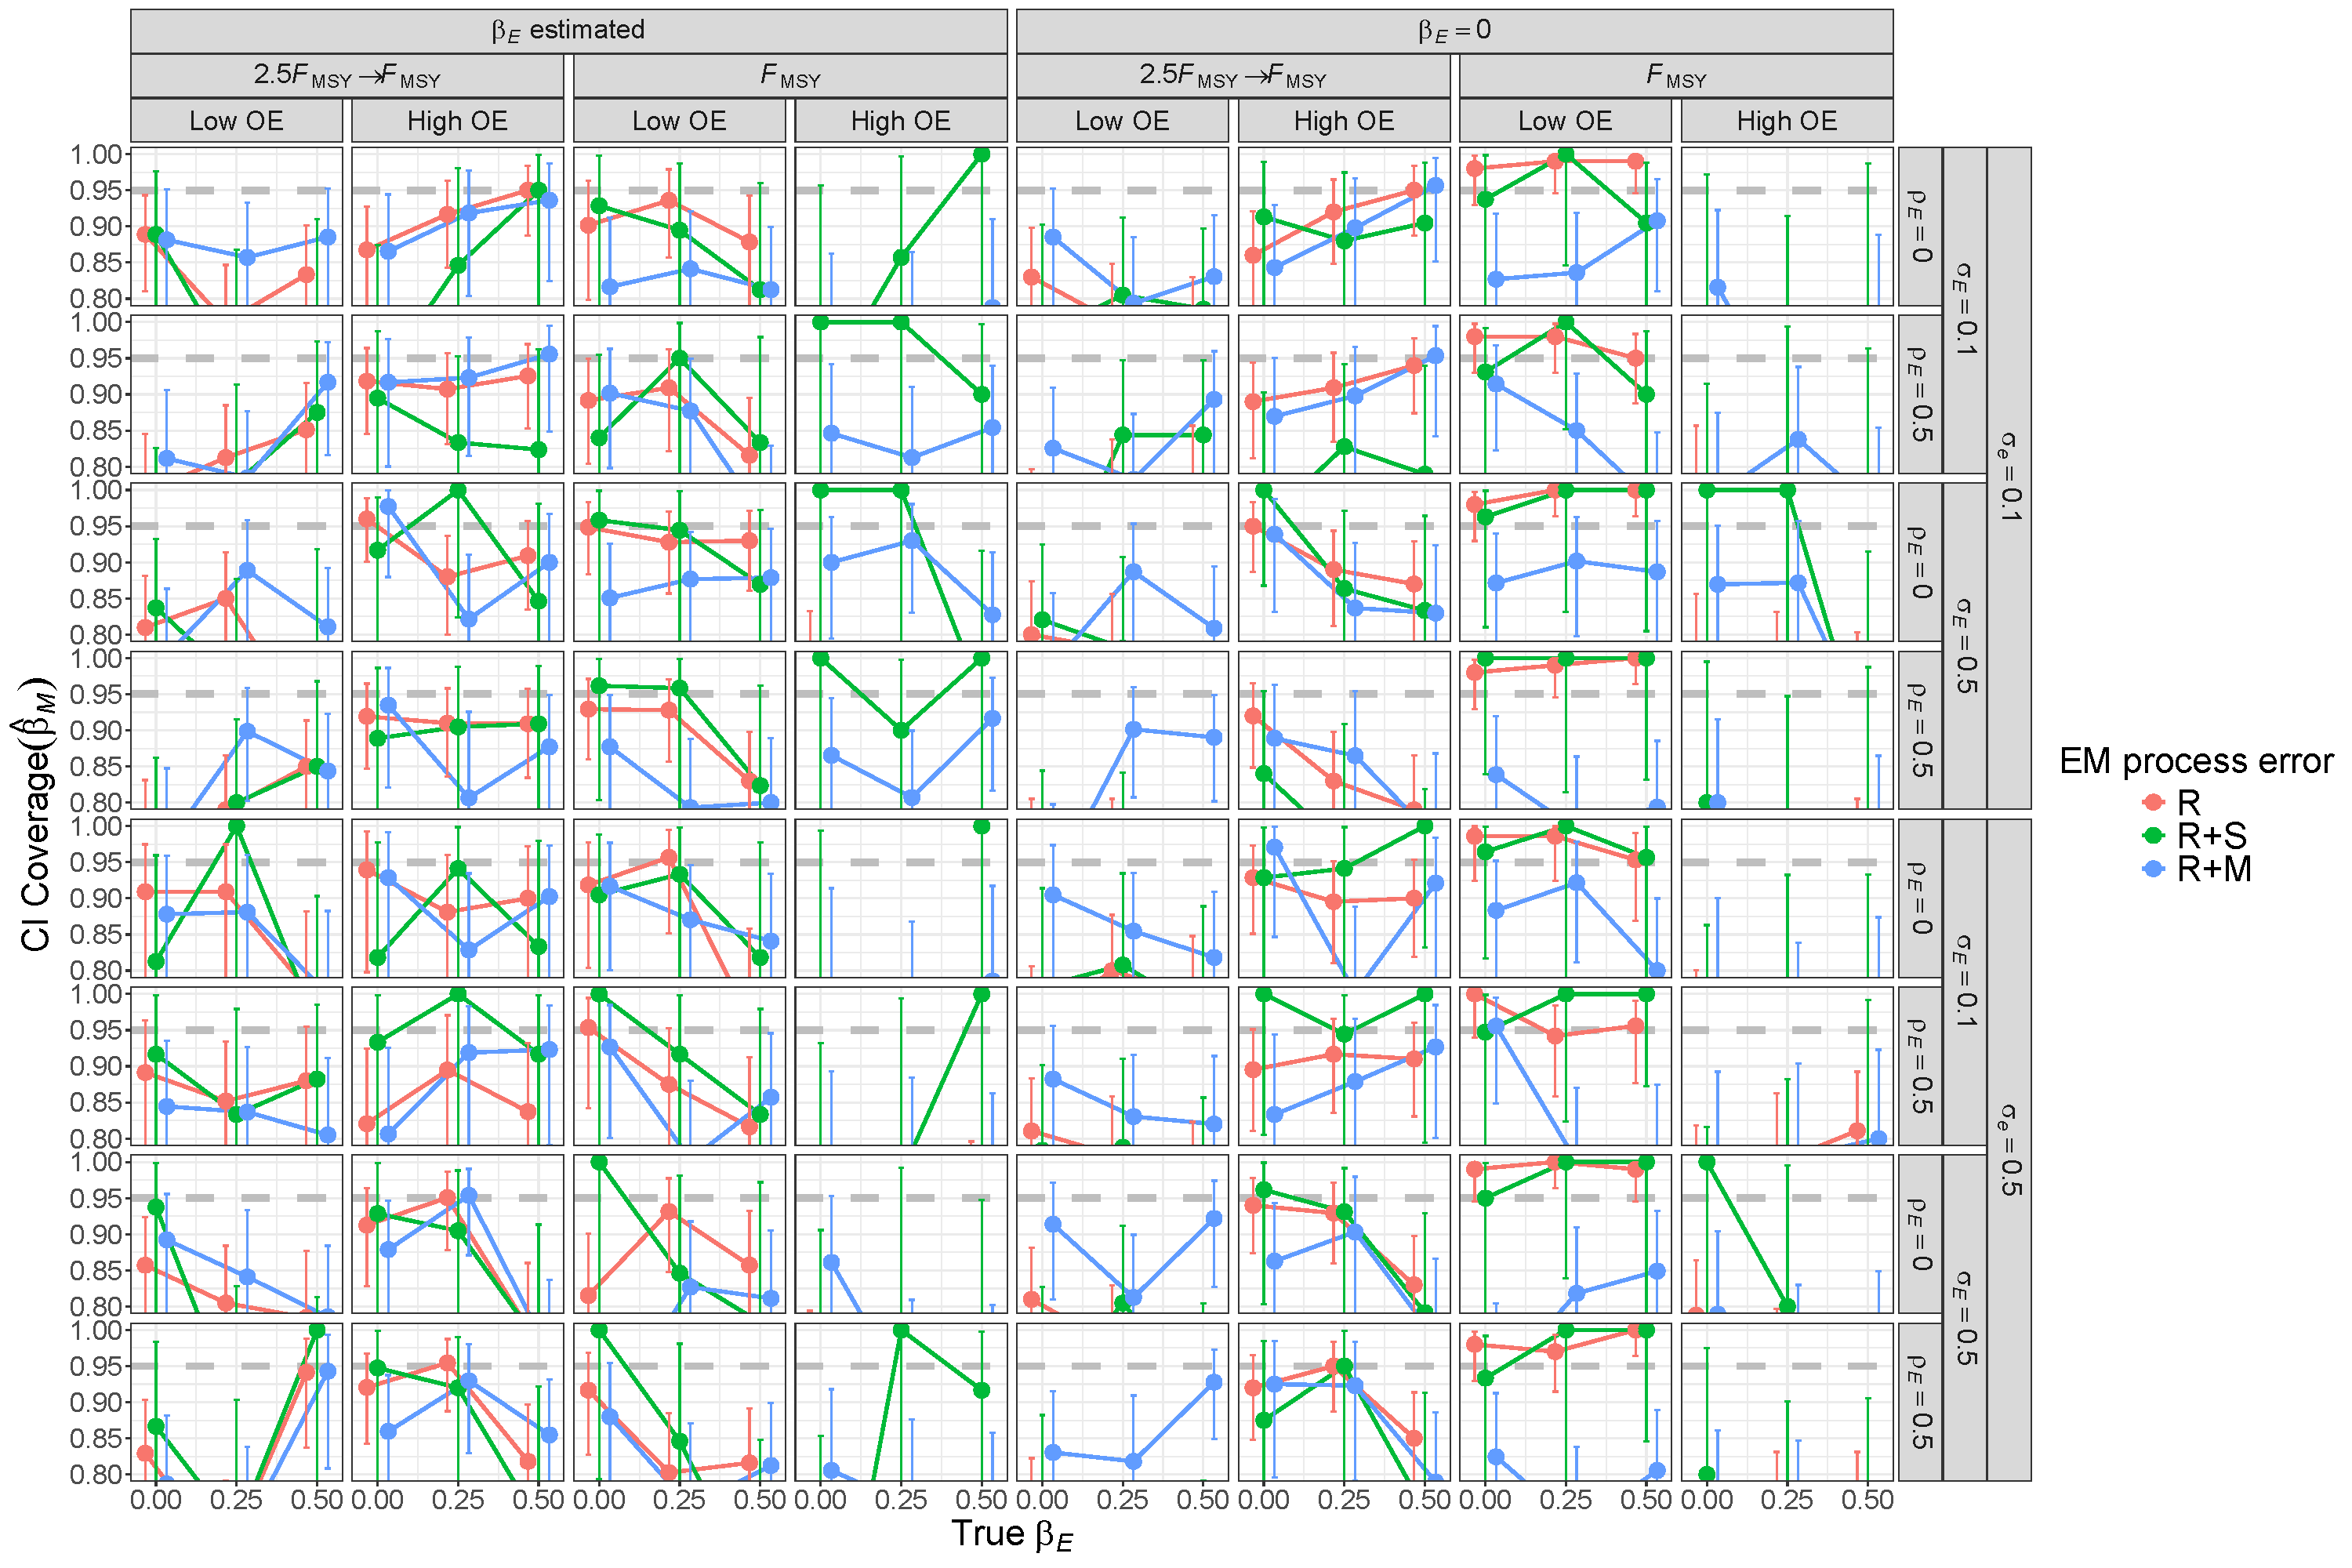
\includegraphics[height = \textheight]{beta_M_CI_coverage_RMom}
\end{center}
\caption{For R+M OMs, probability of 95\% confidence interval for $\beta_M$ containing the true value for EMs with alternative process error assumptions and treatment of covariate effect ($\beta_E = 0$ or estimated). Vertical lines represent 95\% confidence intervals.}\label{beta_M_CI_coverage_RMom}
\end{figure}
\end{landscape}

\hypertarget{median-natural-mortality-parameter-estimate-and-standard-error-example}{%
\subsection*{Median natural mortality parameter estimate and standard error example}\label{median-natural-mortality-parameter-estimate-and-standard-error-example}}
\addcontentsline{toc}{subsection}{Median natural mortality parameter estimate and standard error example}

\begin{landscape}
\begin{figure}
\begin{center}
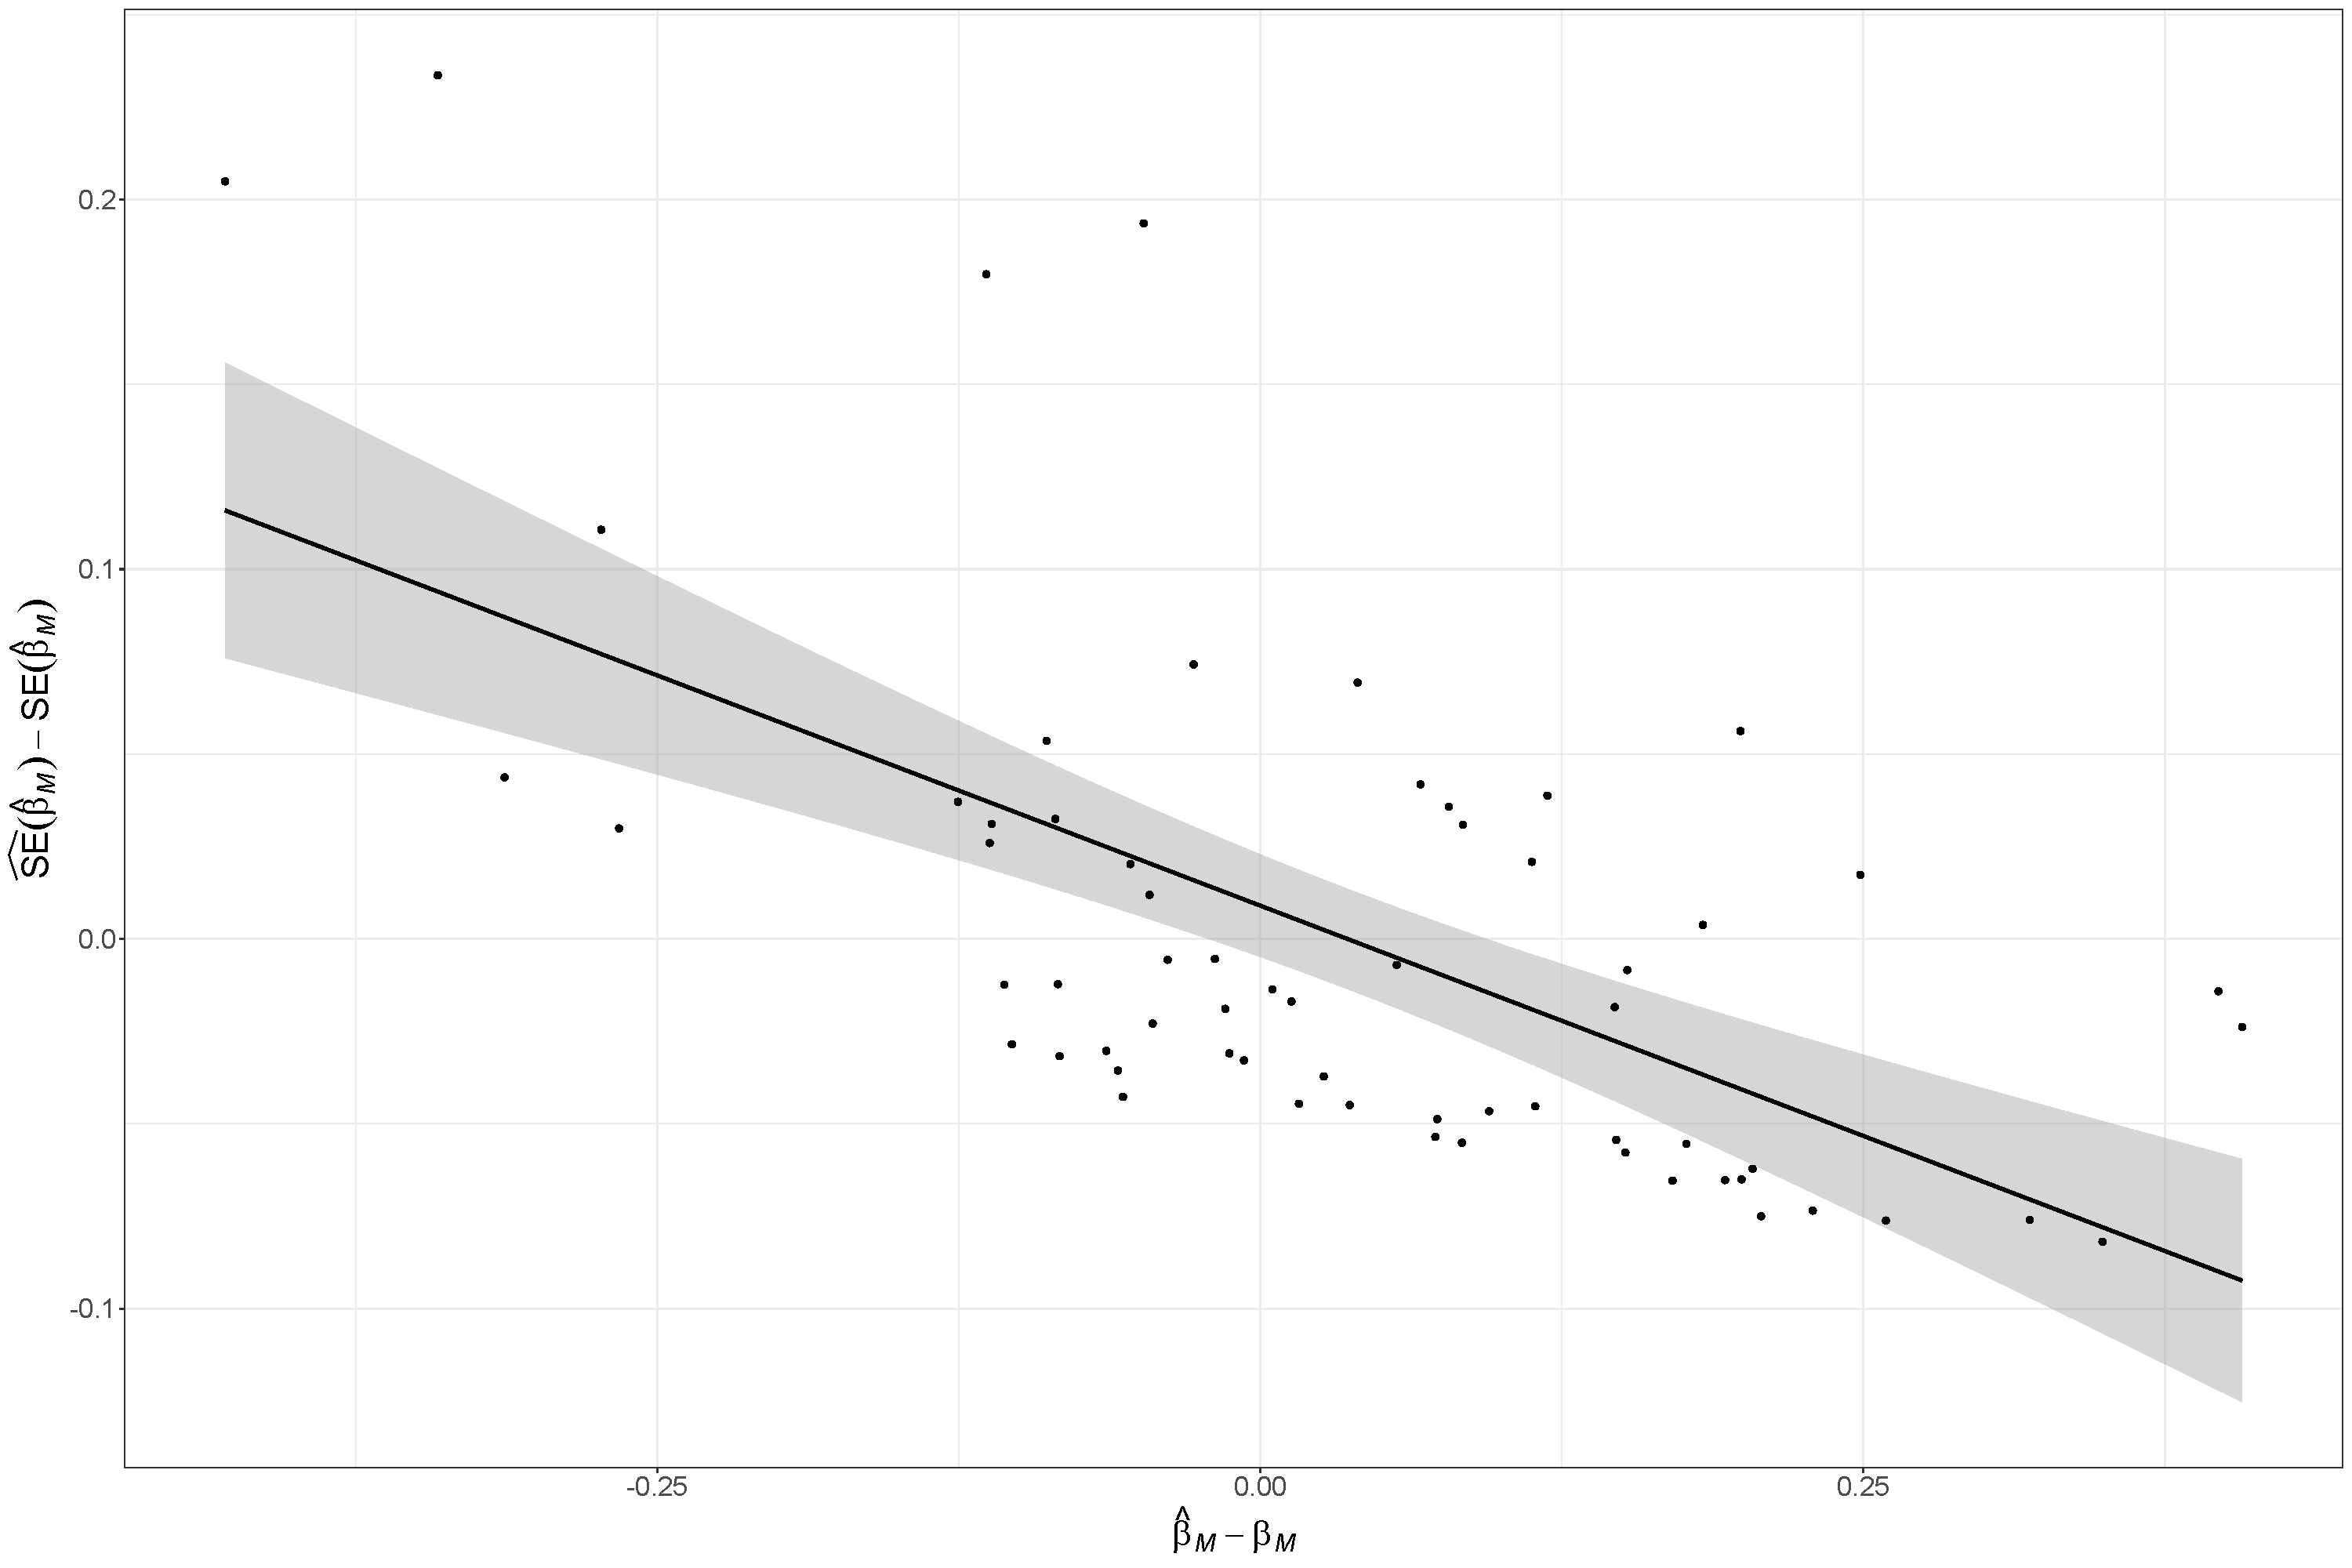
\includegraphics[height = \textheight]{om_69_em_5_beta_M_se_beta_M_lm_plot}
\end{center}
\caption{Negative correlation of $\beta_M$ estimates and Hessian-based standard error estimates for EM that also estimates the covariate effect and has correct R+M process error assumption fitted to simulated data from the OM with R+M process errors, temporal contrast in fishing pressure, low observation uncertainty for both population ($Low OE$) and covariate observations ($\sigma_e = 0.1$), high and uncorrelated temporal variability in the true covariate ($\sigma_E = 0.5$ and $\rho_E = 0$), and the strongest covariate effect on natural mortality ($\beta_E = 0.5$).}\label{ex_lm_beta_M_SE_beta_M}
\end{figure}
\end{landscape}

\hypertarget{median-natural-mortality-parameter-rmse}{%
\subsection*{Median Natural mortality parameter RMSE}\label{median-natural-mortality-parameter-rmse}}
\addcontentsline{toc}{subsection}{Median Natural mortality parameter RMSE}

\begin{landscape}
\begin{figure}
\begin{center}
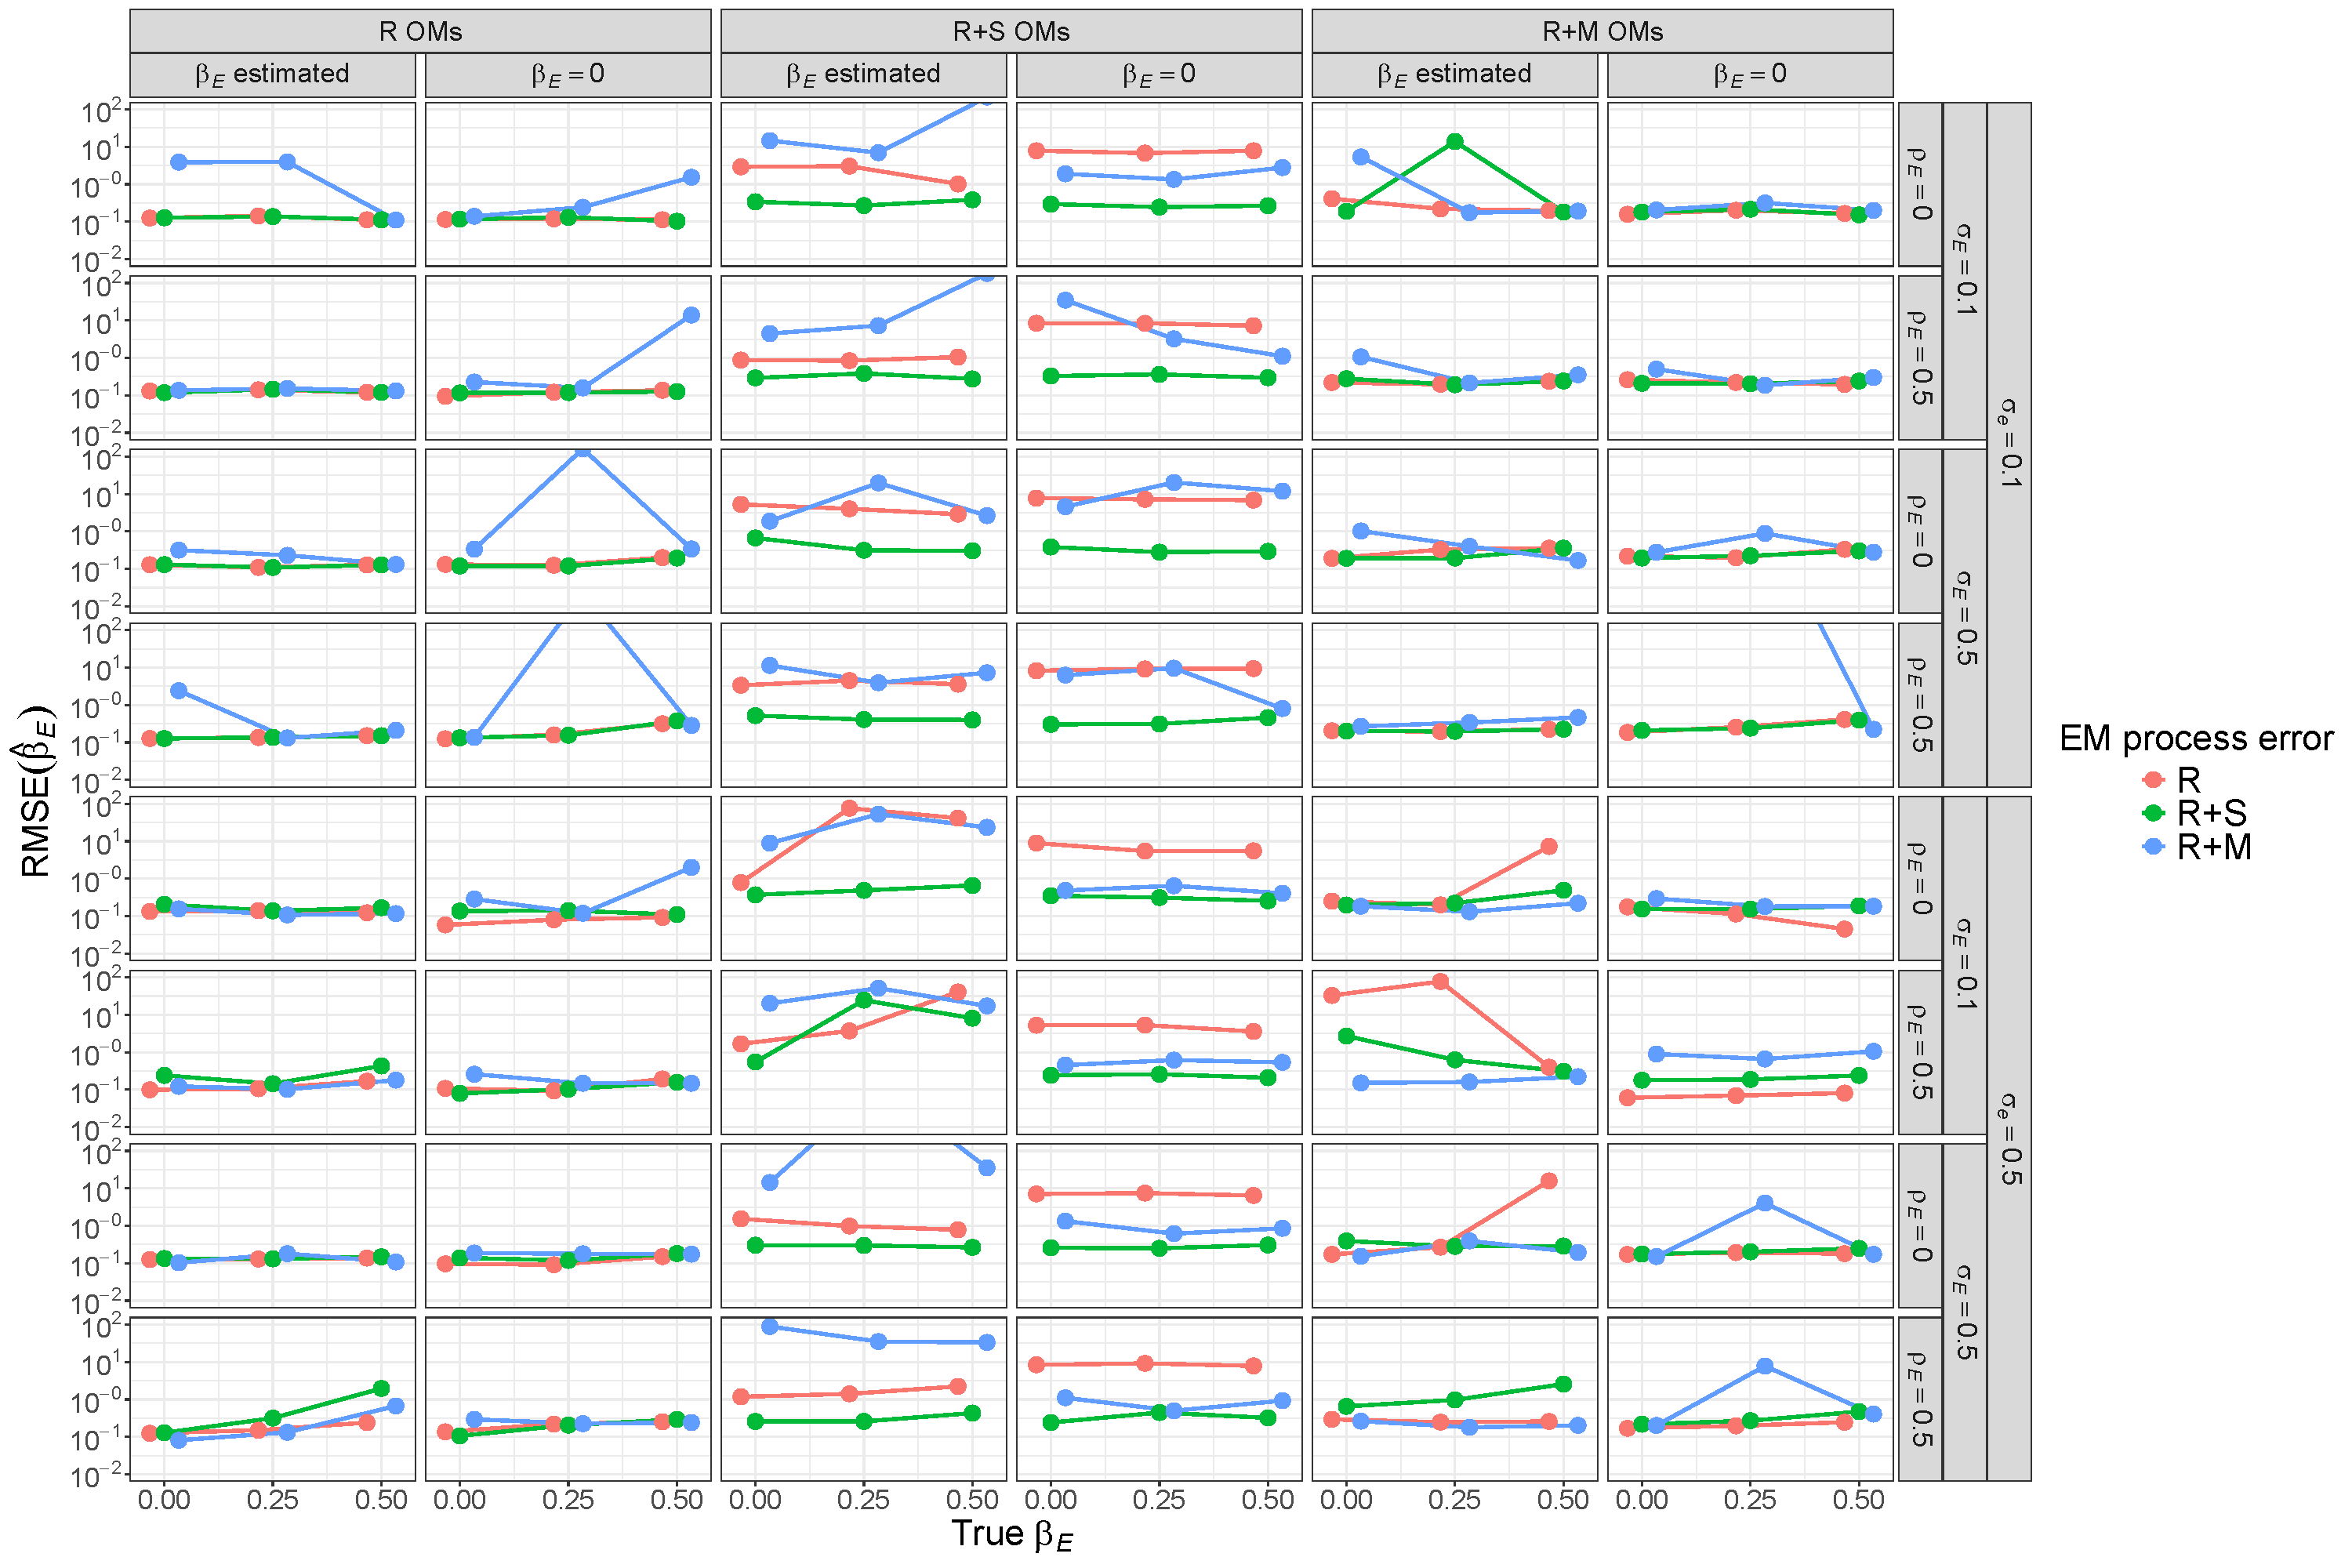
\includegraphics[height = \textheight]{beta_M_rmse_main}
\end{center}
\caption{Root mean square error  (RMSE) of estimates of  $\beta_M$ from fitting EMs with alternative process error assumptions and treatment of covariate effect ($\beta_E = 0$ or estimated). All OMs had low observation error for population observations and contrast in fishing mortality.}\label{beta_M_rmse}
\end{figure}
\end{landscape}

\begin{landscape}
\begin{figure}
\begin{center}
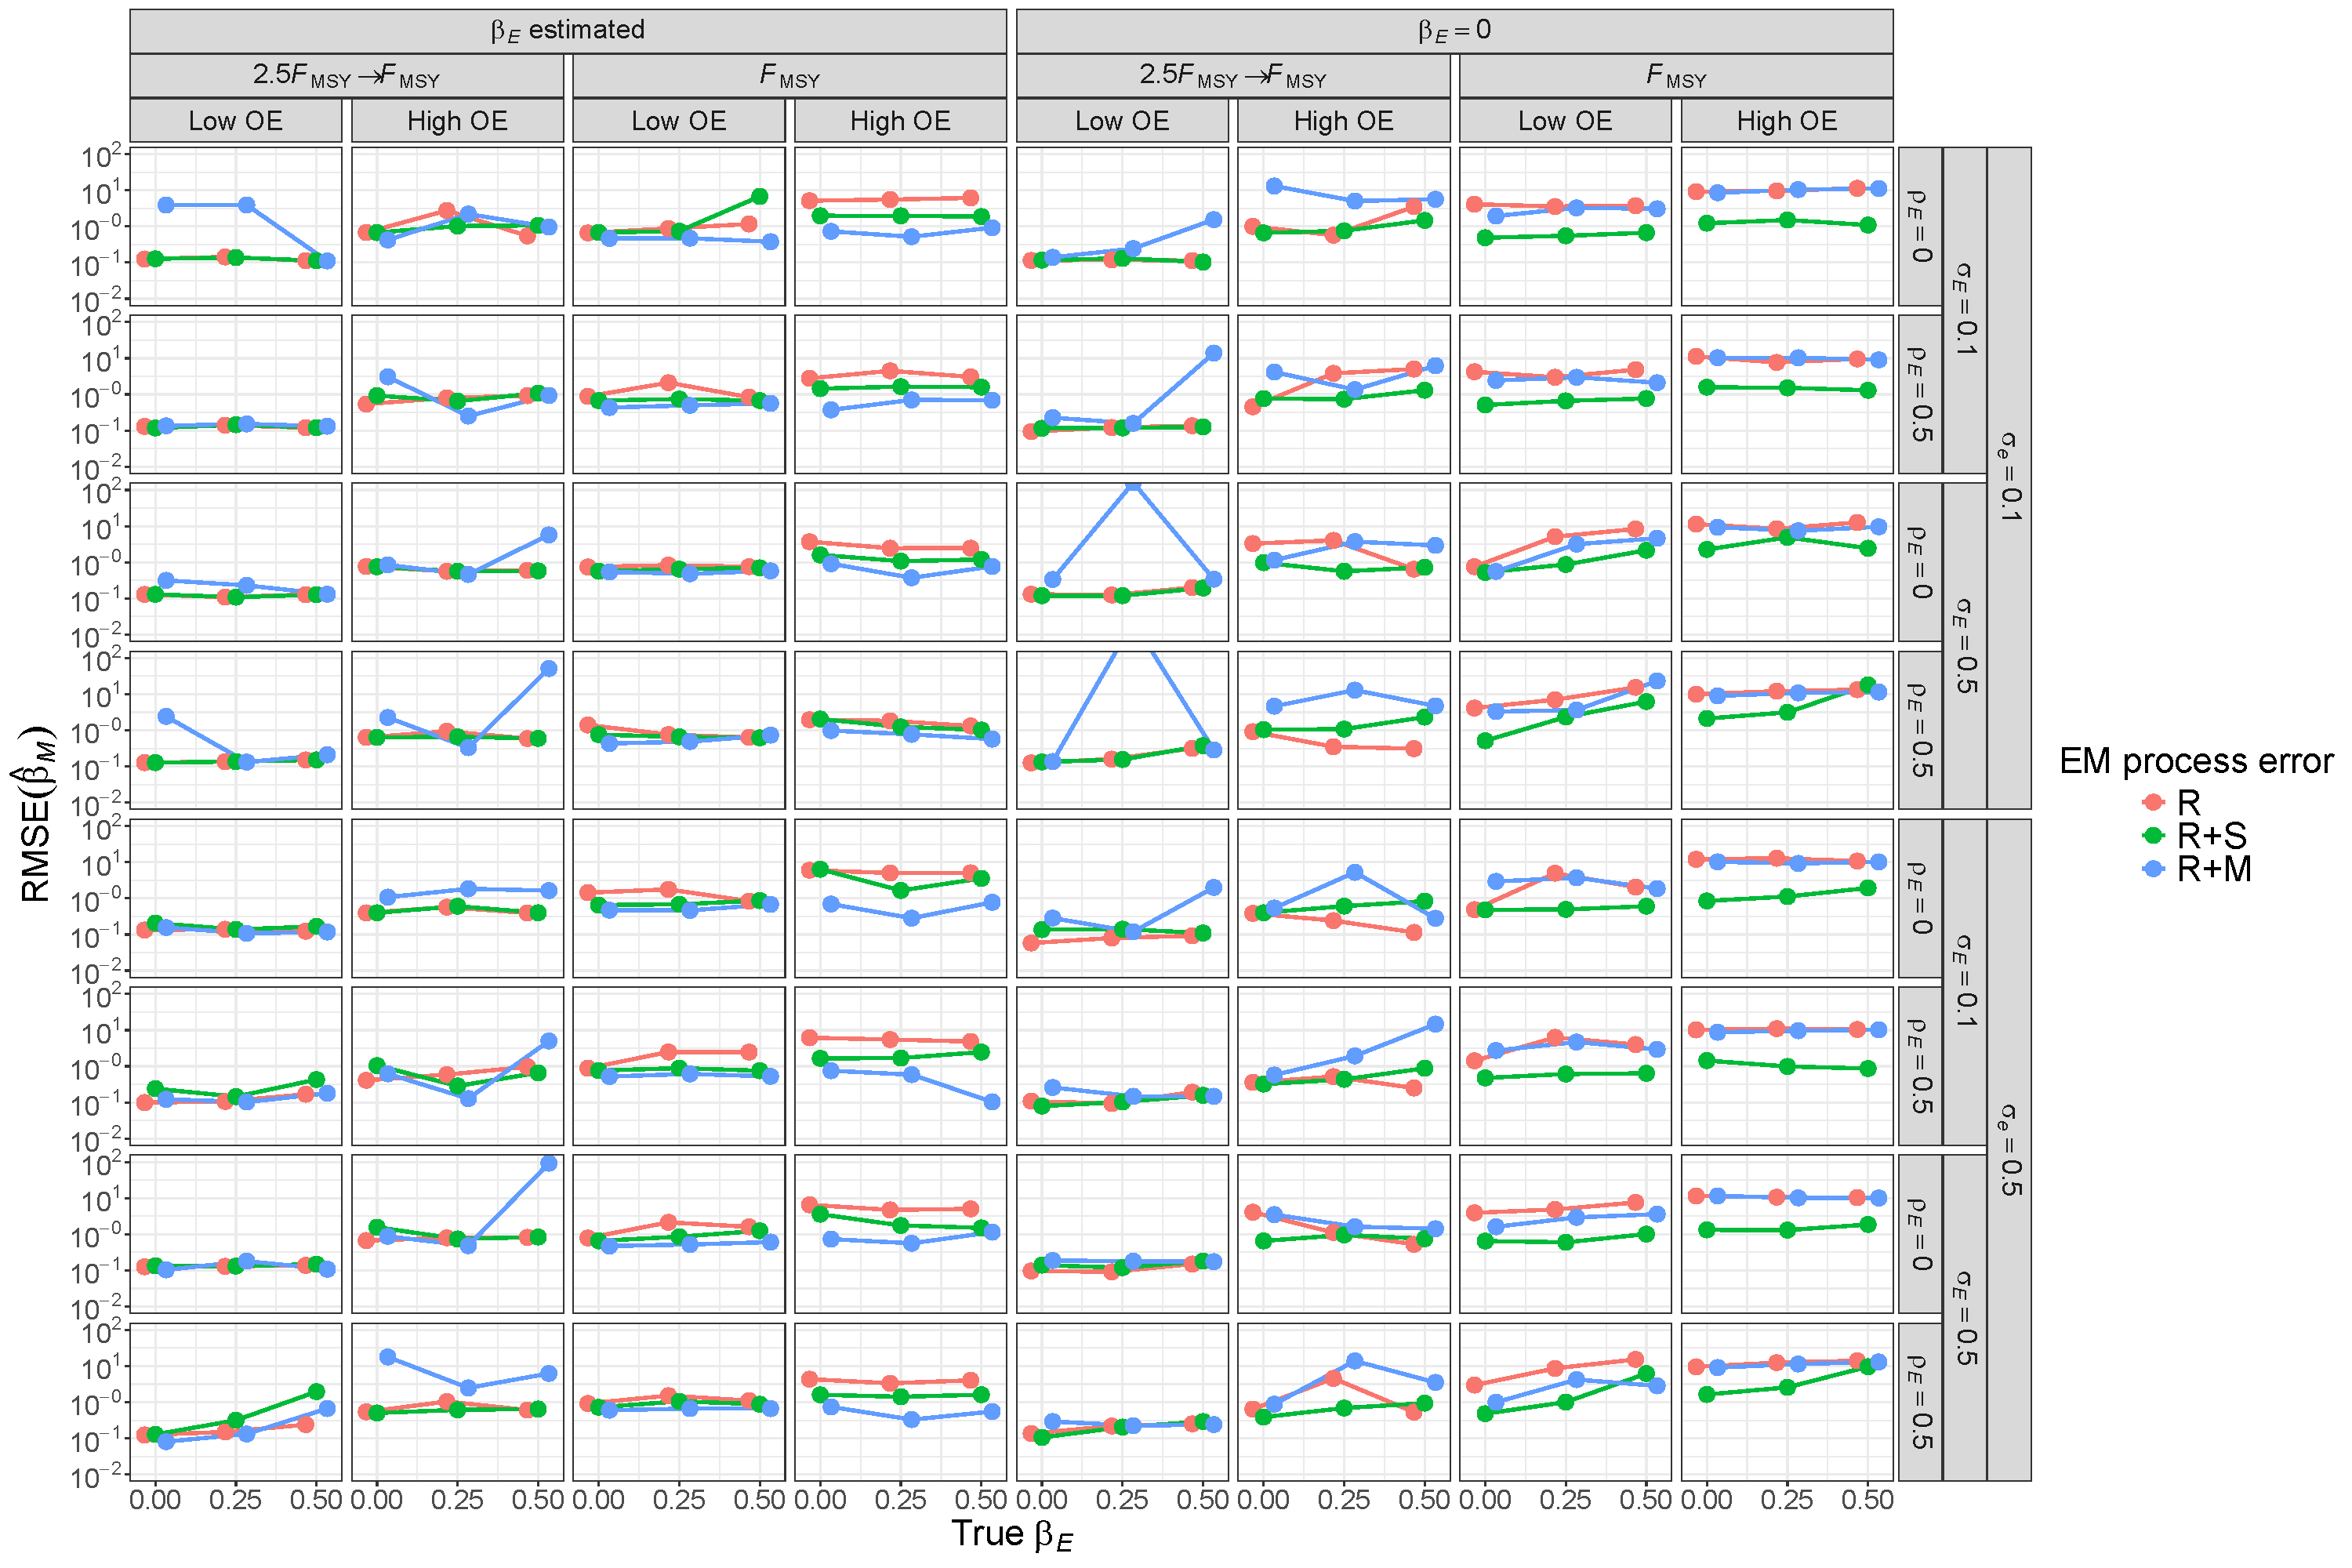
\includegraphics[height = \textheight]{beta_M_rmse_Rom}
\end{center}
\caption{For R OMs, root mean square error (RMSE) of estimates of  $\beta_M$ from fitting EMs with alternative process error assumptions and treatment of covariate effect ($\beta_E = 0$ or estimated).}\label{beta_M_rmse_Rom}
\end{figure}
\end{landscape}

\begin{landscape}
\begin{figure}
\begin{center}
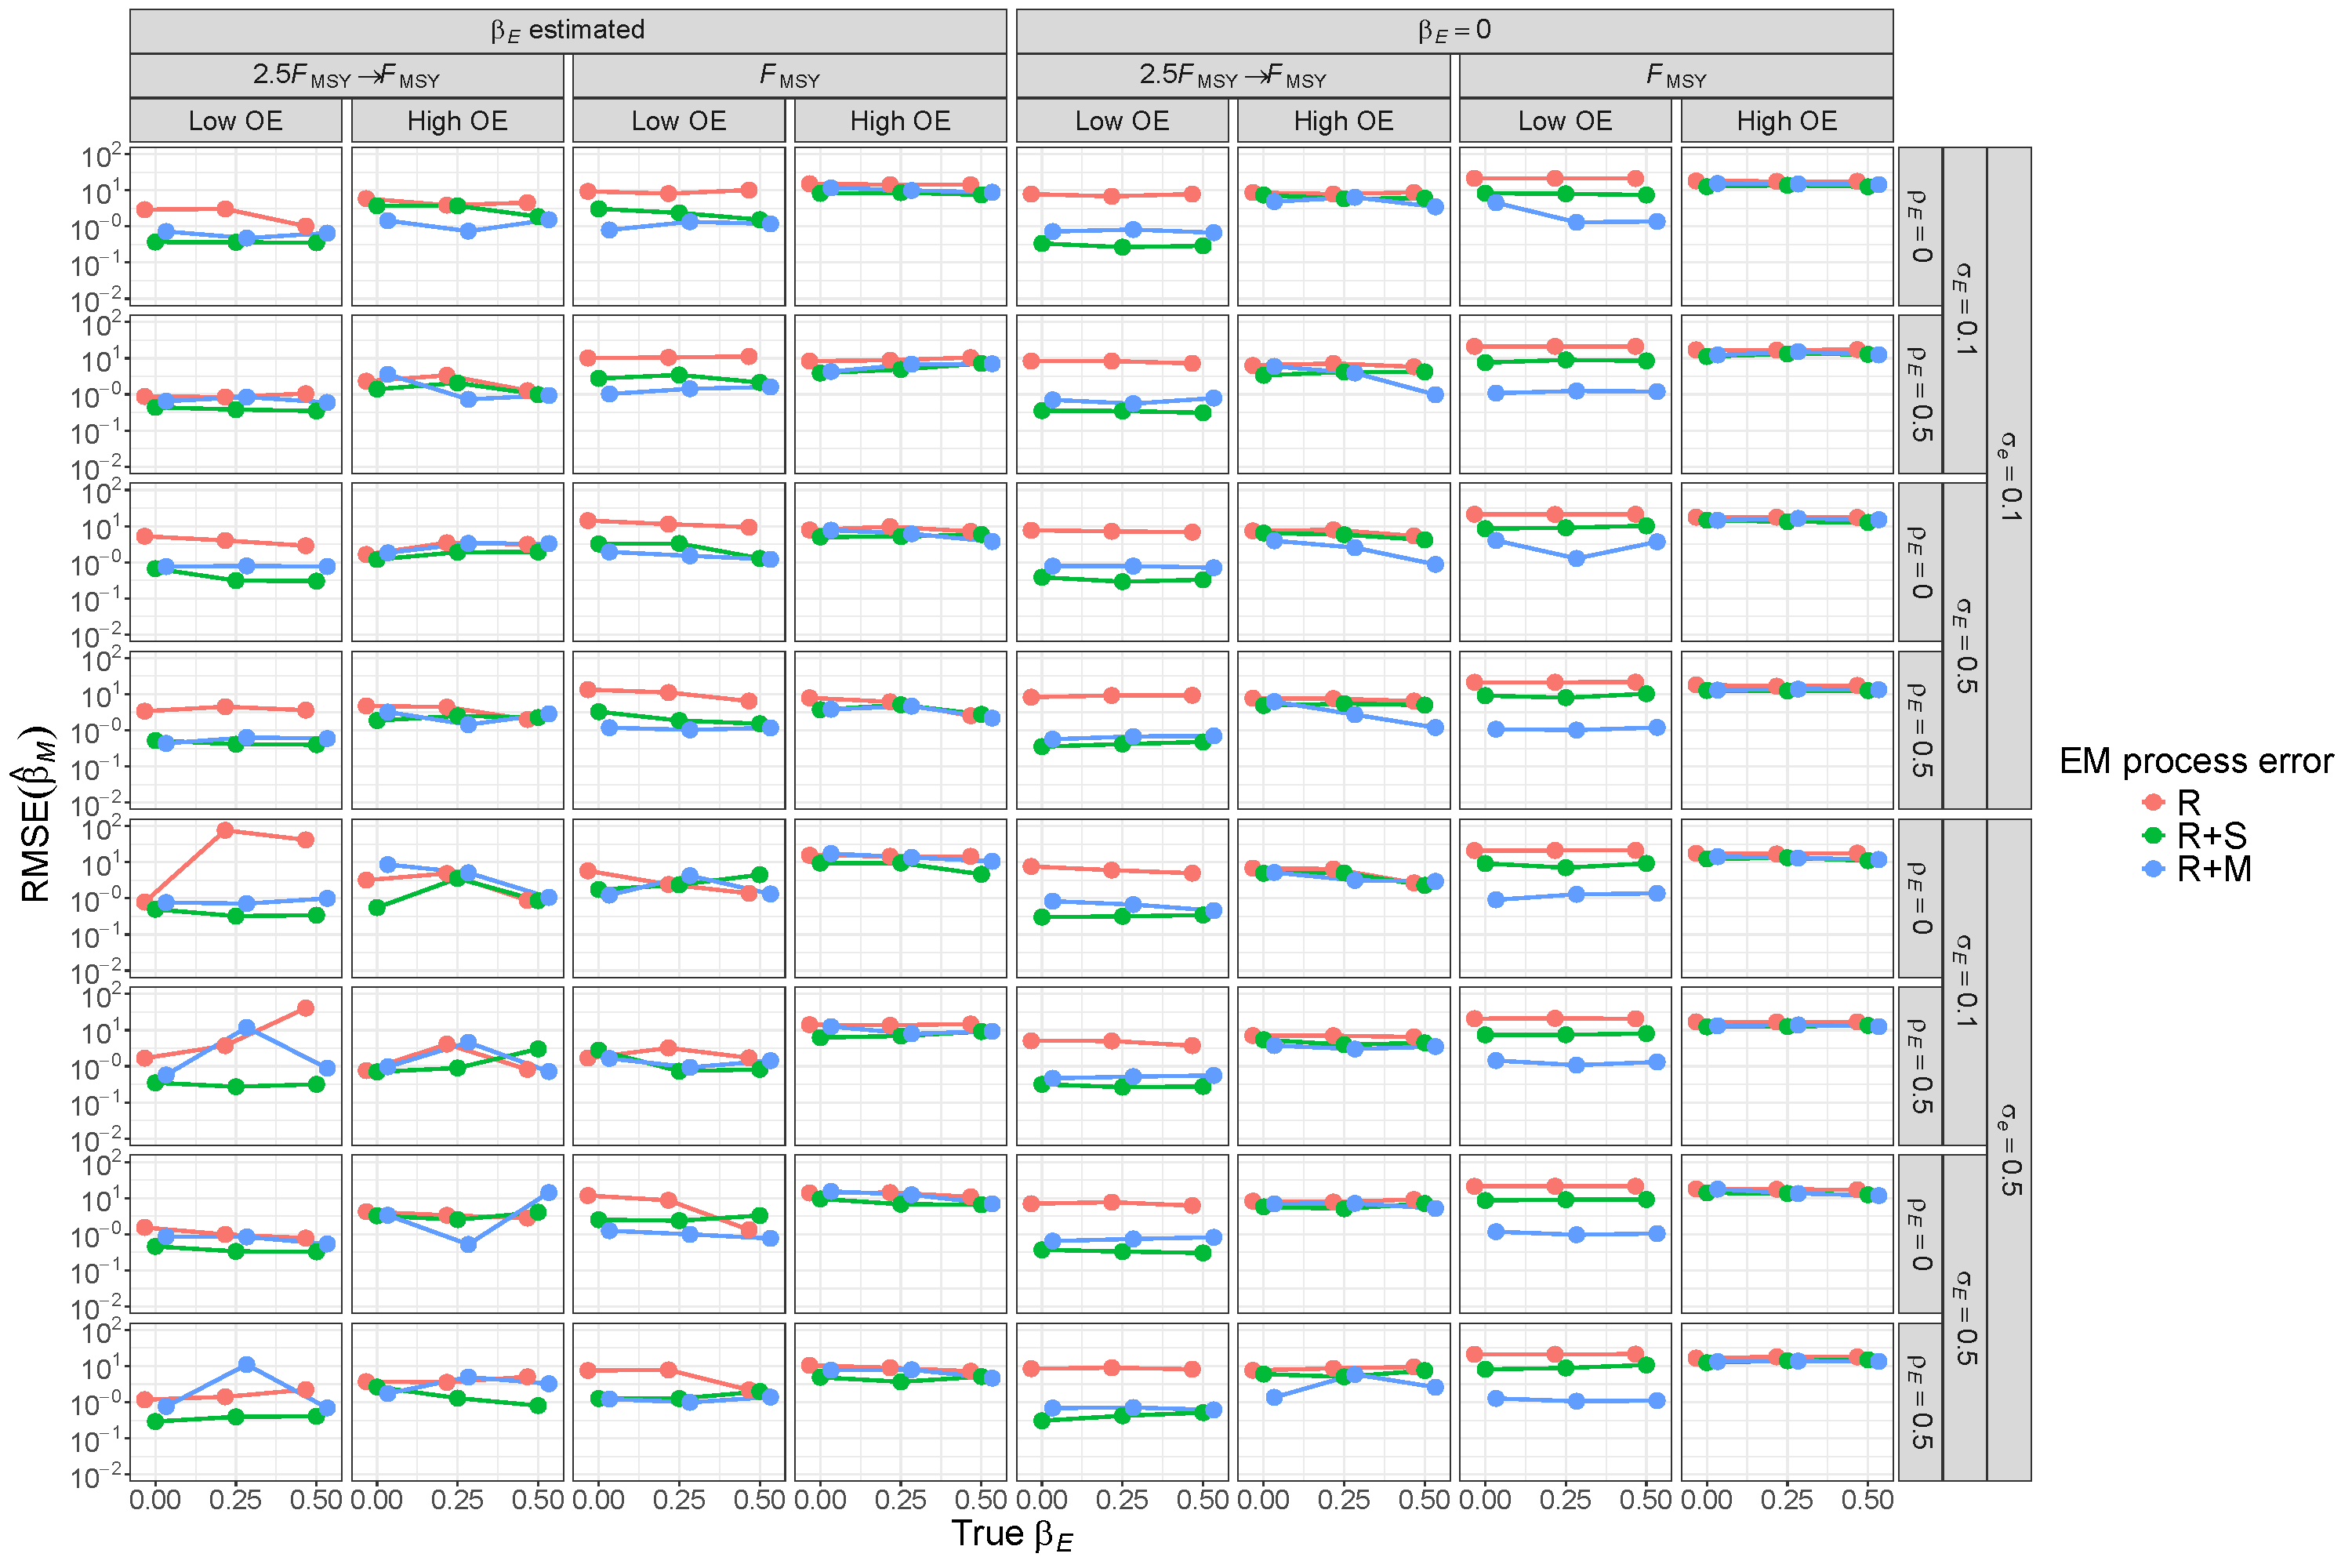
\includegraphics[height = \textheight]{beta_M_rmse_RSom}
\end{center}
\caption{For R+S OMs, root mean square error (RMSE) of estimates of  $\beta_M$ from fitting EMs with alternative process error assumptions and treatment of covariate effect ($\beta_E = 0$ or estimated).}\label{beta_M_rmse_RSom}
\end{figure}
\end{landscape}

\begin{landscape}
\begin{figure}
\begin{center}
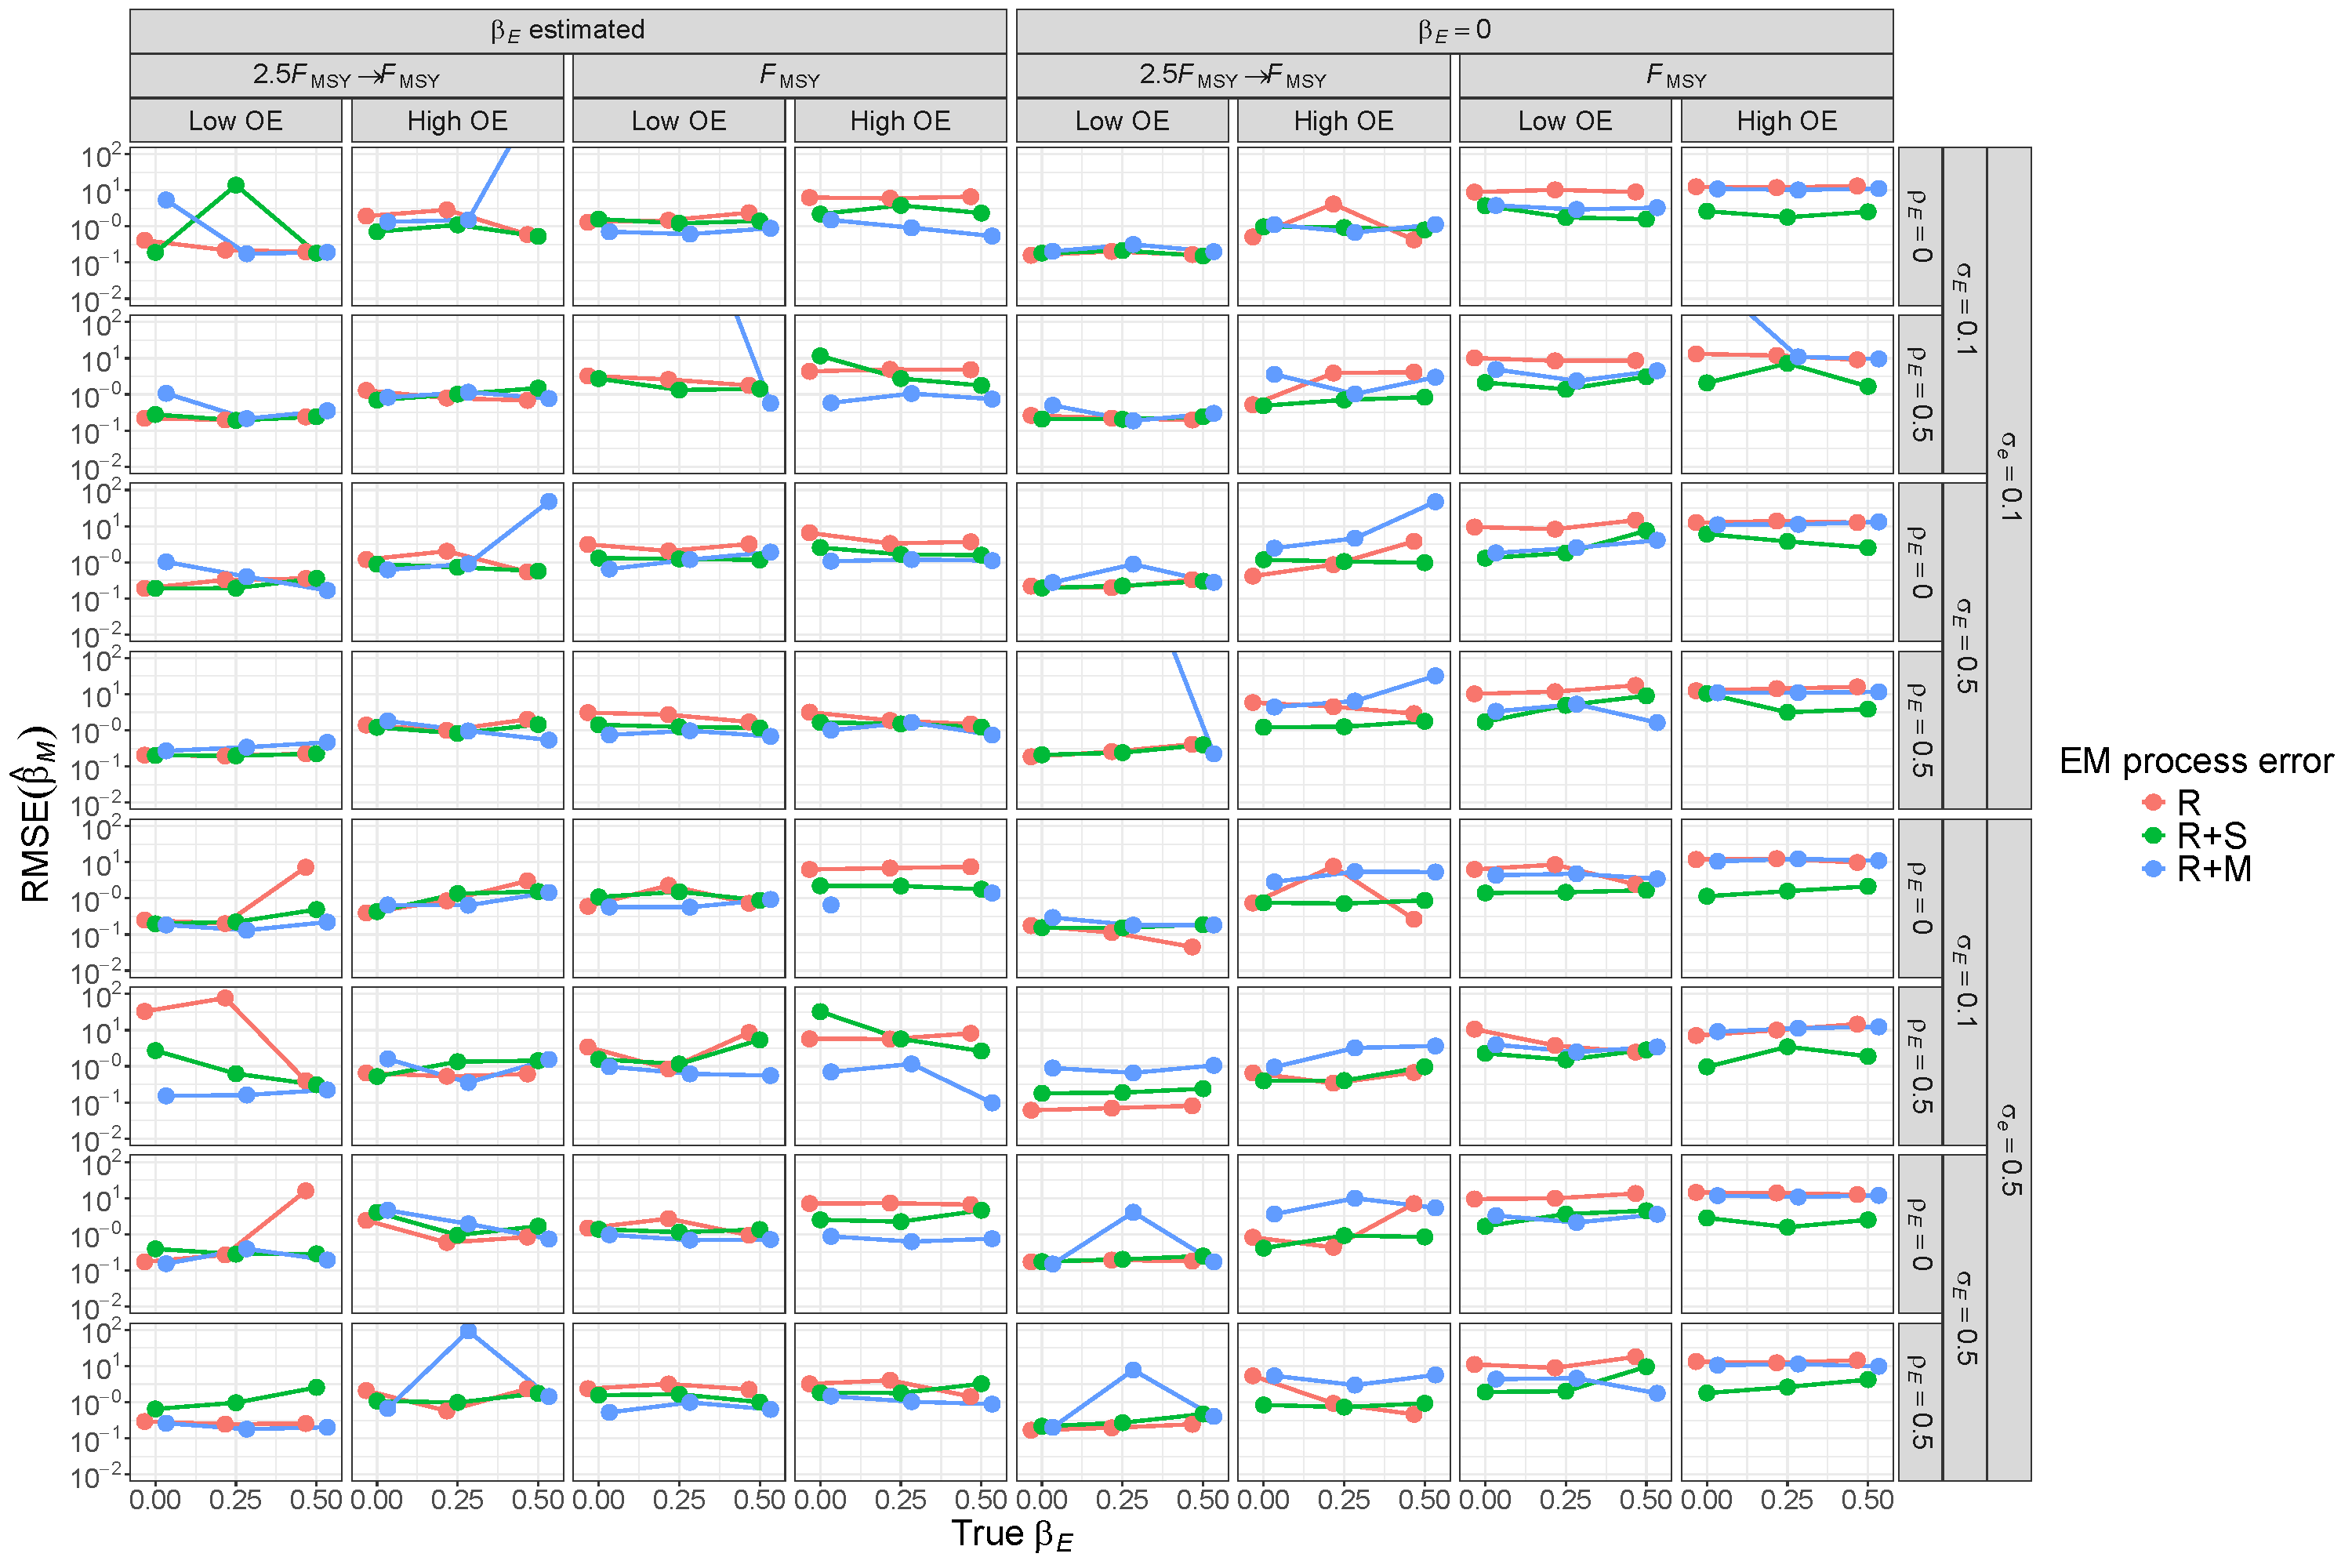
\includegraphics[height = \textheight]{beta_M_rmse_RMom}
\end{center}
\caption{For R+M OMs, root mean square error (RMSE) of estimates of  $\beta_M$ from fitting EMs with alternative process error assumptions and treatment of covariate effect ($\beta_E = 0$ or estimated).}\label{beta_M_rmse_RMom}
\end{figure}
\end{landscape}

\hypertarget{terminal-year-natural-mortality-bias}{%
\subsection*{Terminal year natural mortality bias}\label{terminal-year-natural-mortality-bias}}
\addcontentsline{toc}{subsection}{Terminal year natural mortality bias}

\begin{landscape}
\begin{figure}
\begin{center}
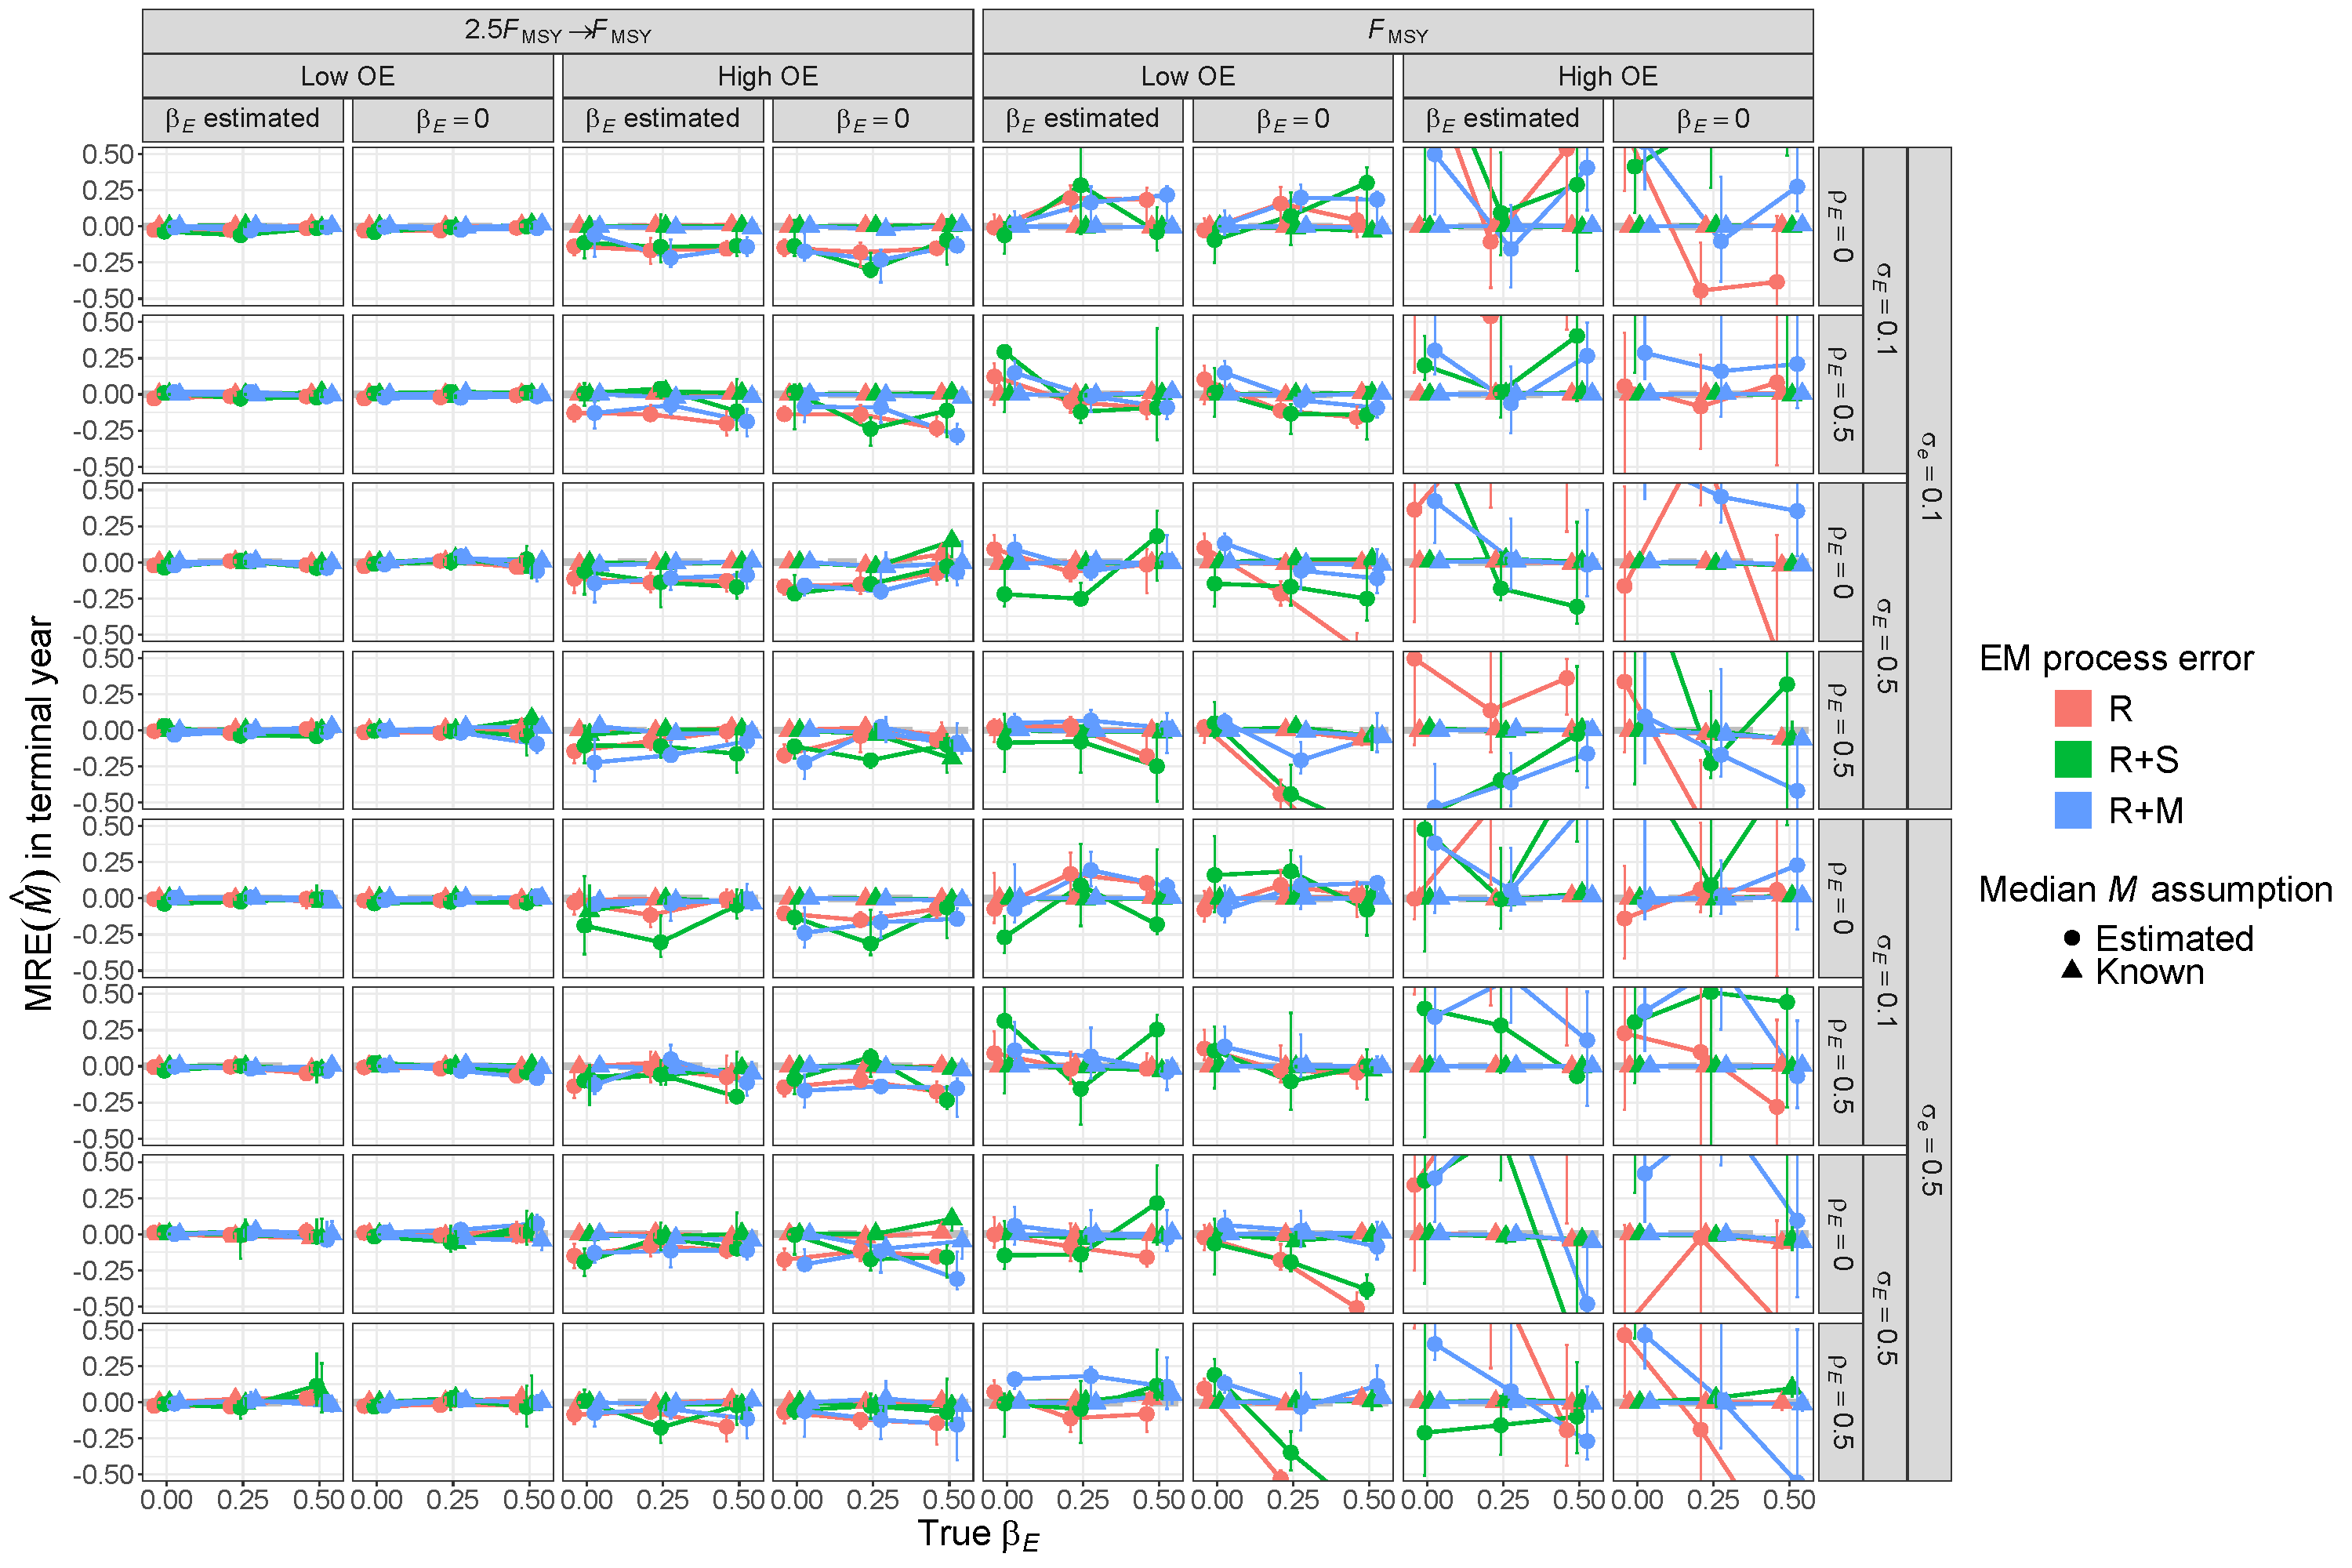
\includegraphics[height = \textheight]{terminal_year_M_bias_Rom}
\end{center}
\caption{For R OMs, median relative error (MRE) of estimates of natural mortality rate in the terminal year for EMs with alternative process error assumptions, treatment of covariate effect ($\beta_E = 0$ or estimated), and treatment of median natural mortality parameter ($\beta_M$ estimated or known).}\label{terminal_M_bias_Rom}
\end{figure}
\end{landscape}

\begin{landscape}
\begin{figure}
\begin{center}
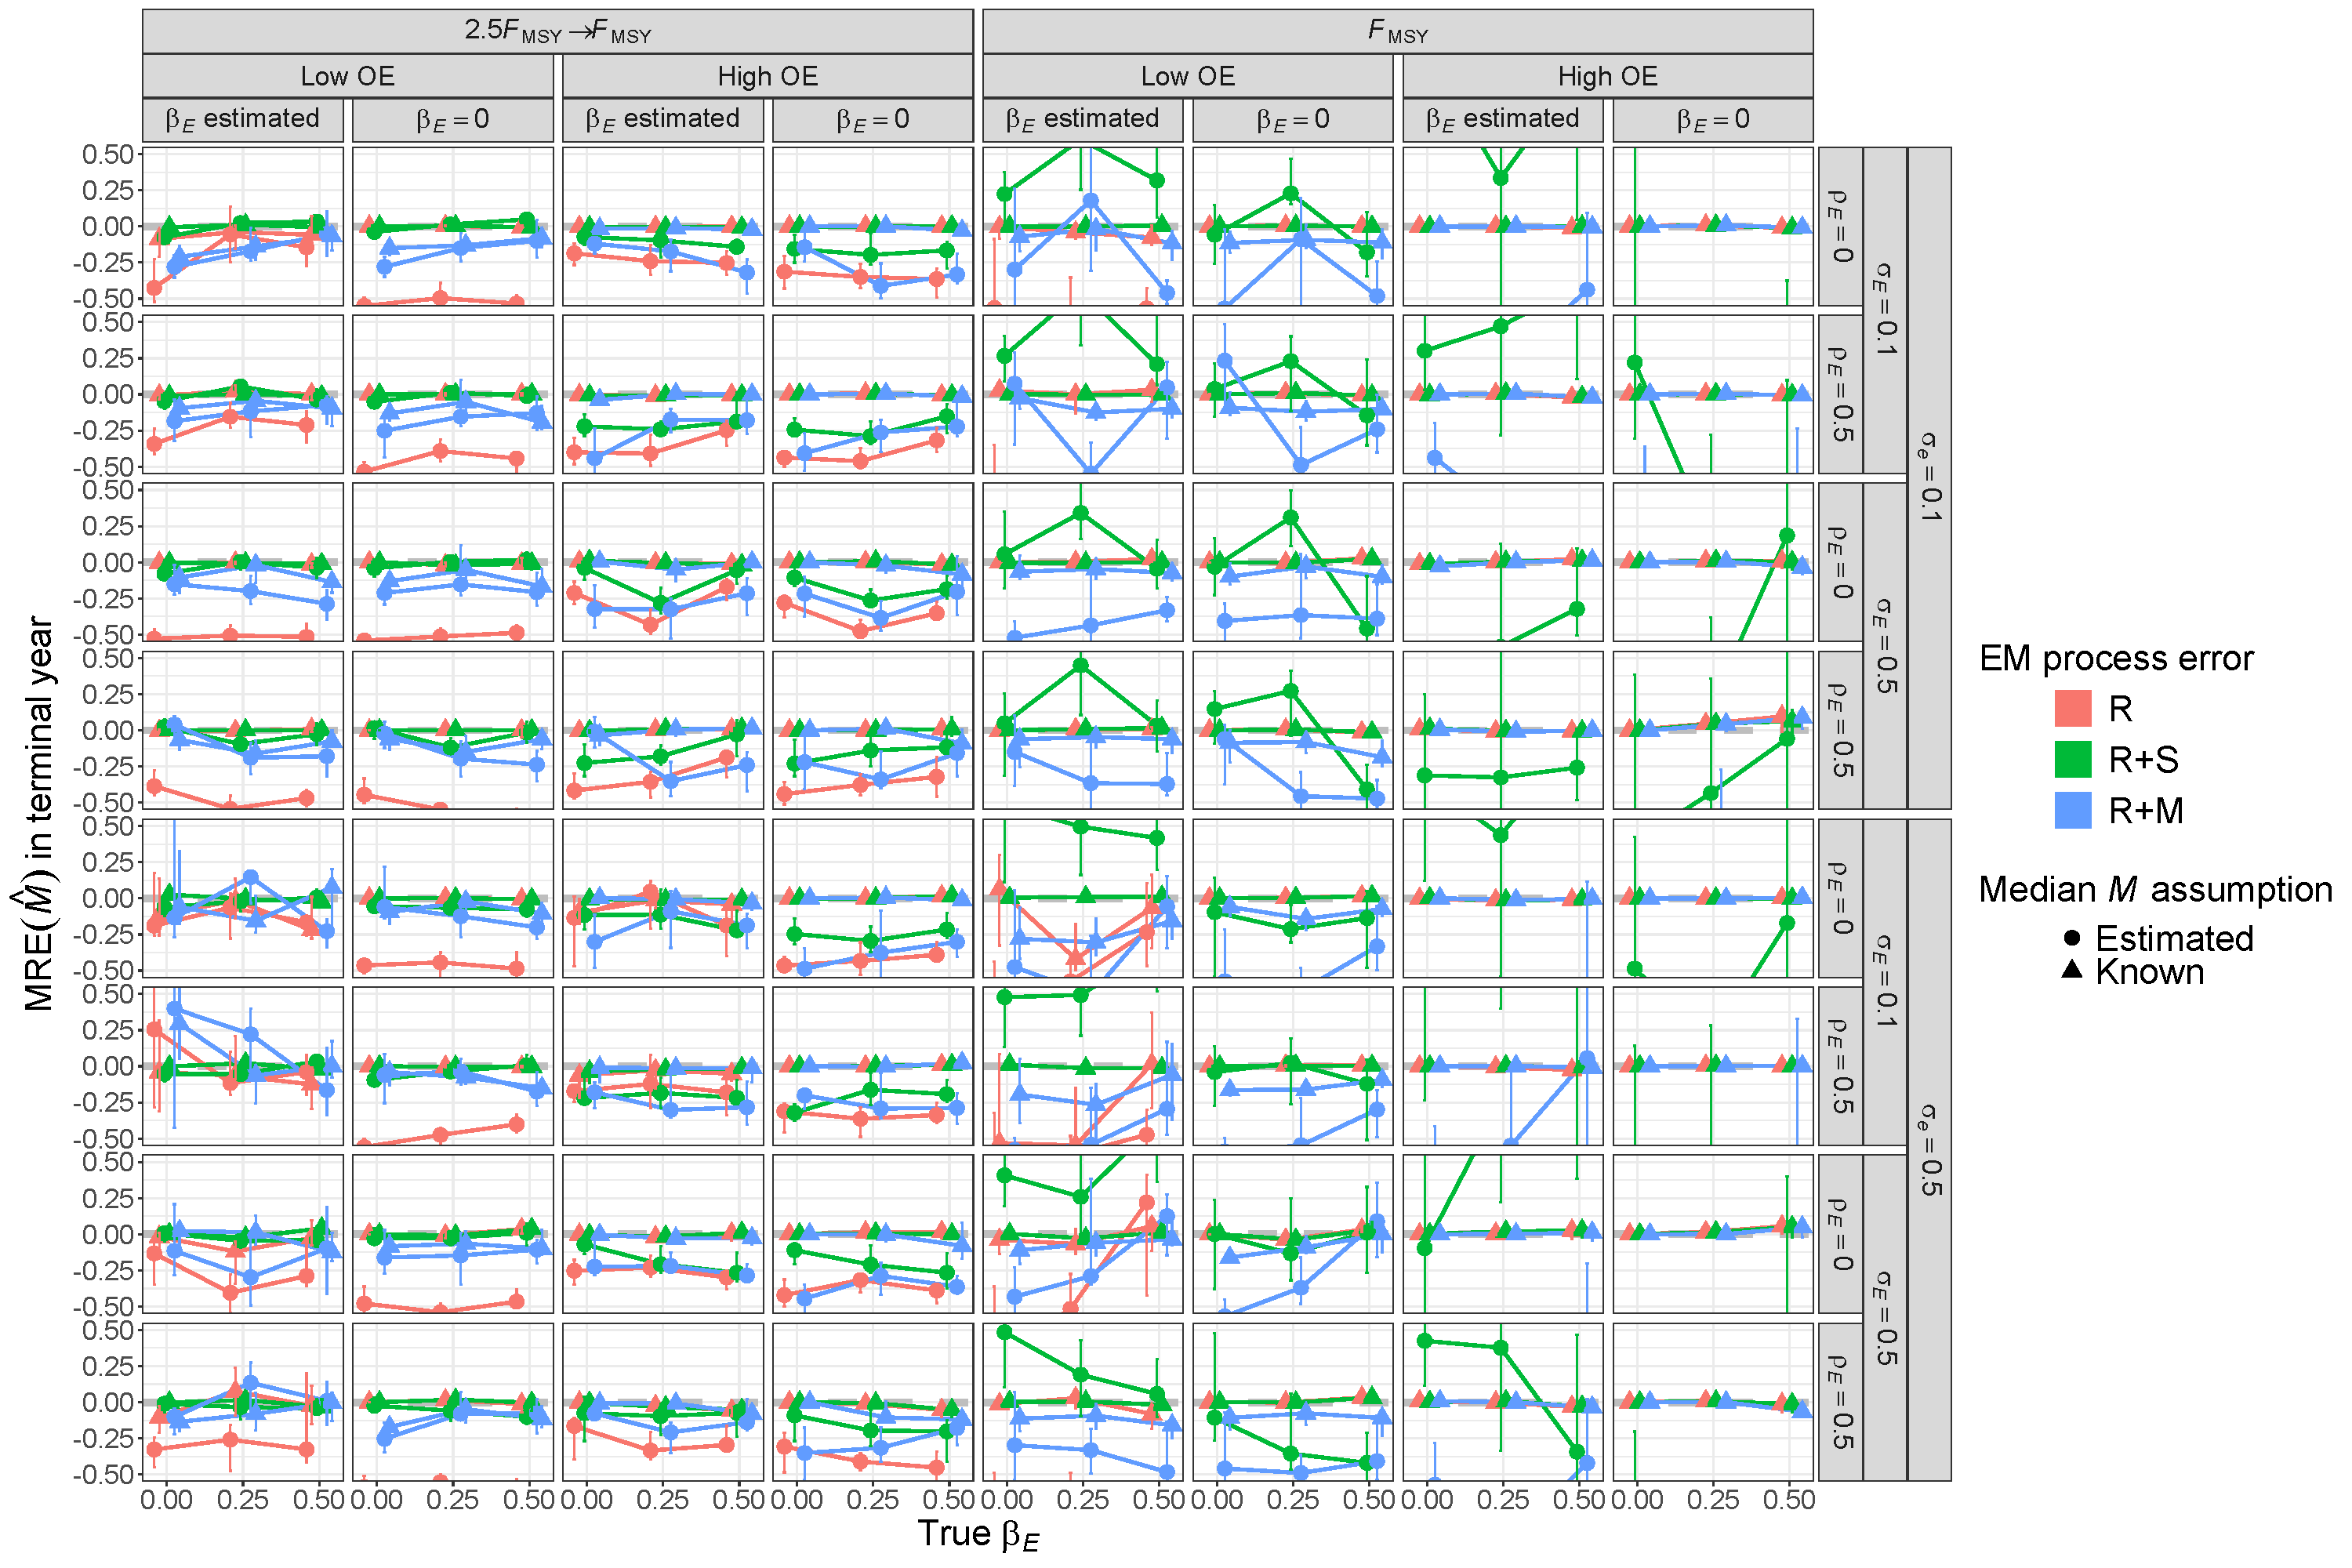
\includegraphics[height = \textheight]{terminal_year_M_bias_RSom}
\end{center}
\caption{For R+S OMs, median relative error (MRE) of estimates of natural mortality rate in the terminal year for EMs with alternative process error assumptions, treatment of covariate effect ($\beta_E = 0$ or estimated), and treatment of median natural mortality parameter ($\beta_M$ estimated or known).}\label{terminal_M_bias_RSom}
\end{figure}
\end{landscape}

\begin{landscape}
\begin{figure}
\begin{center}
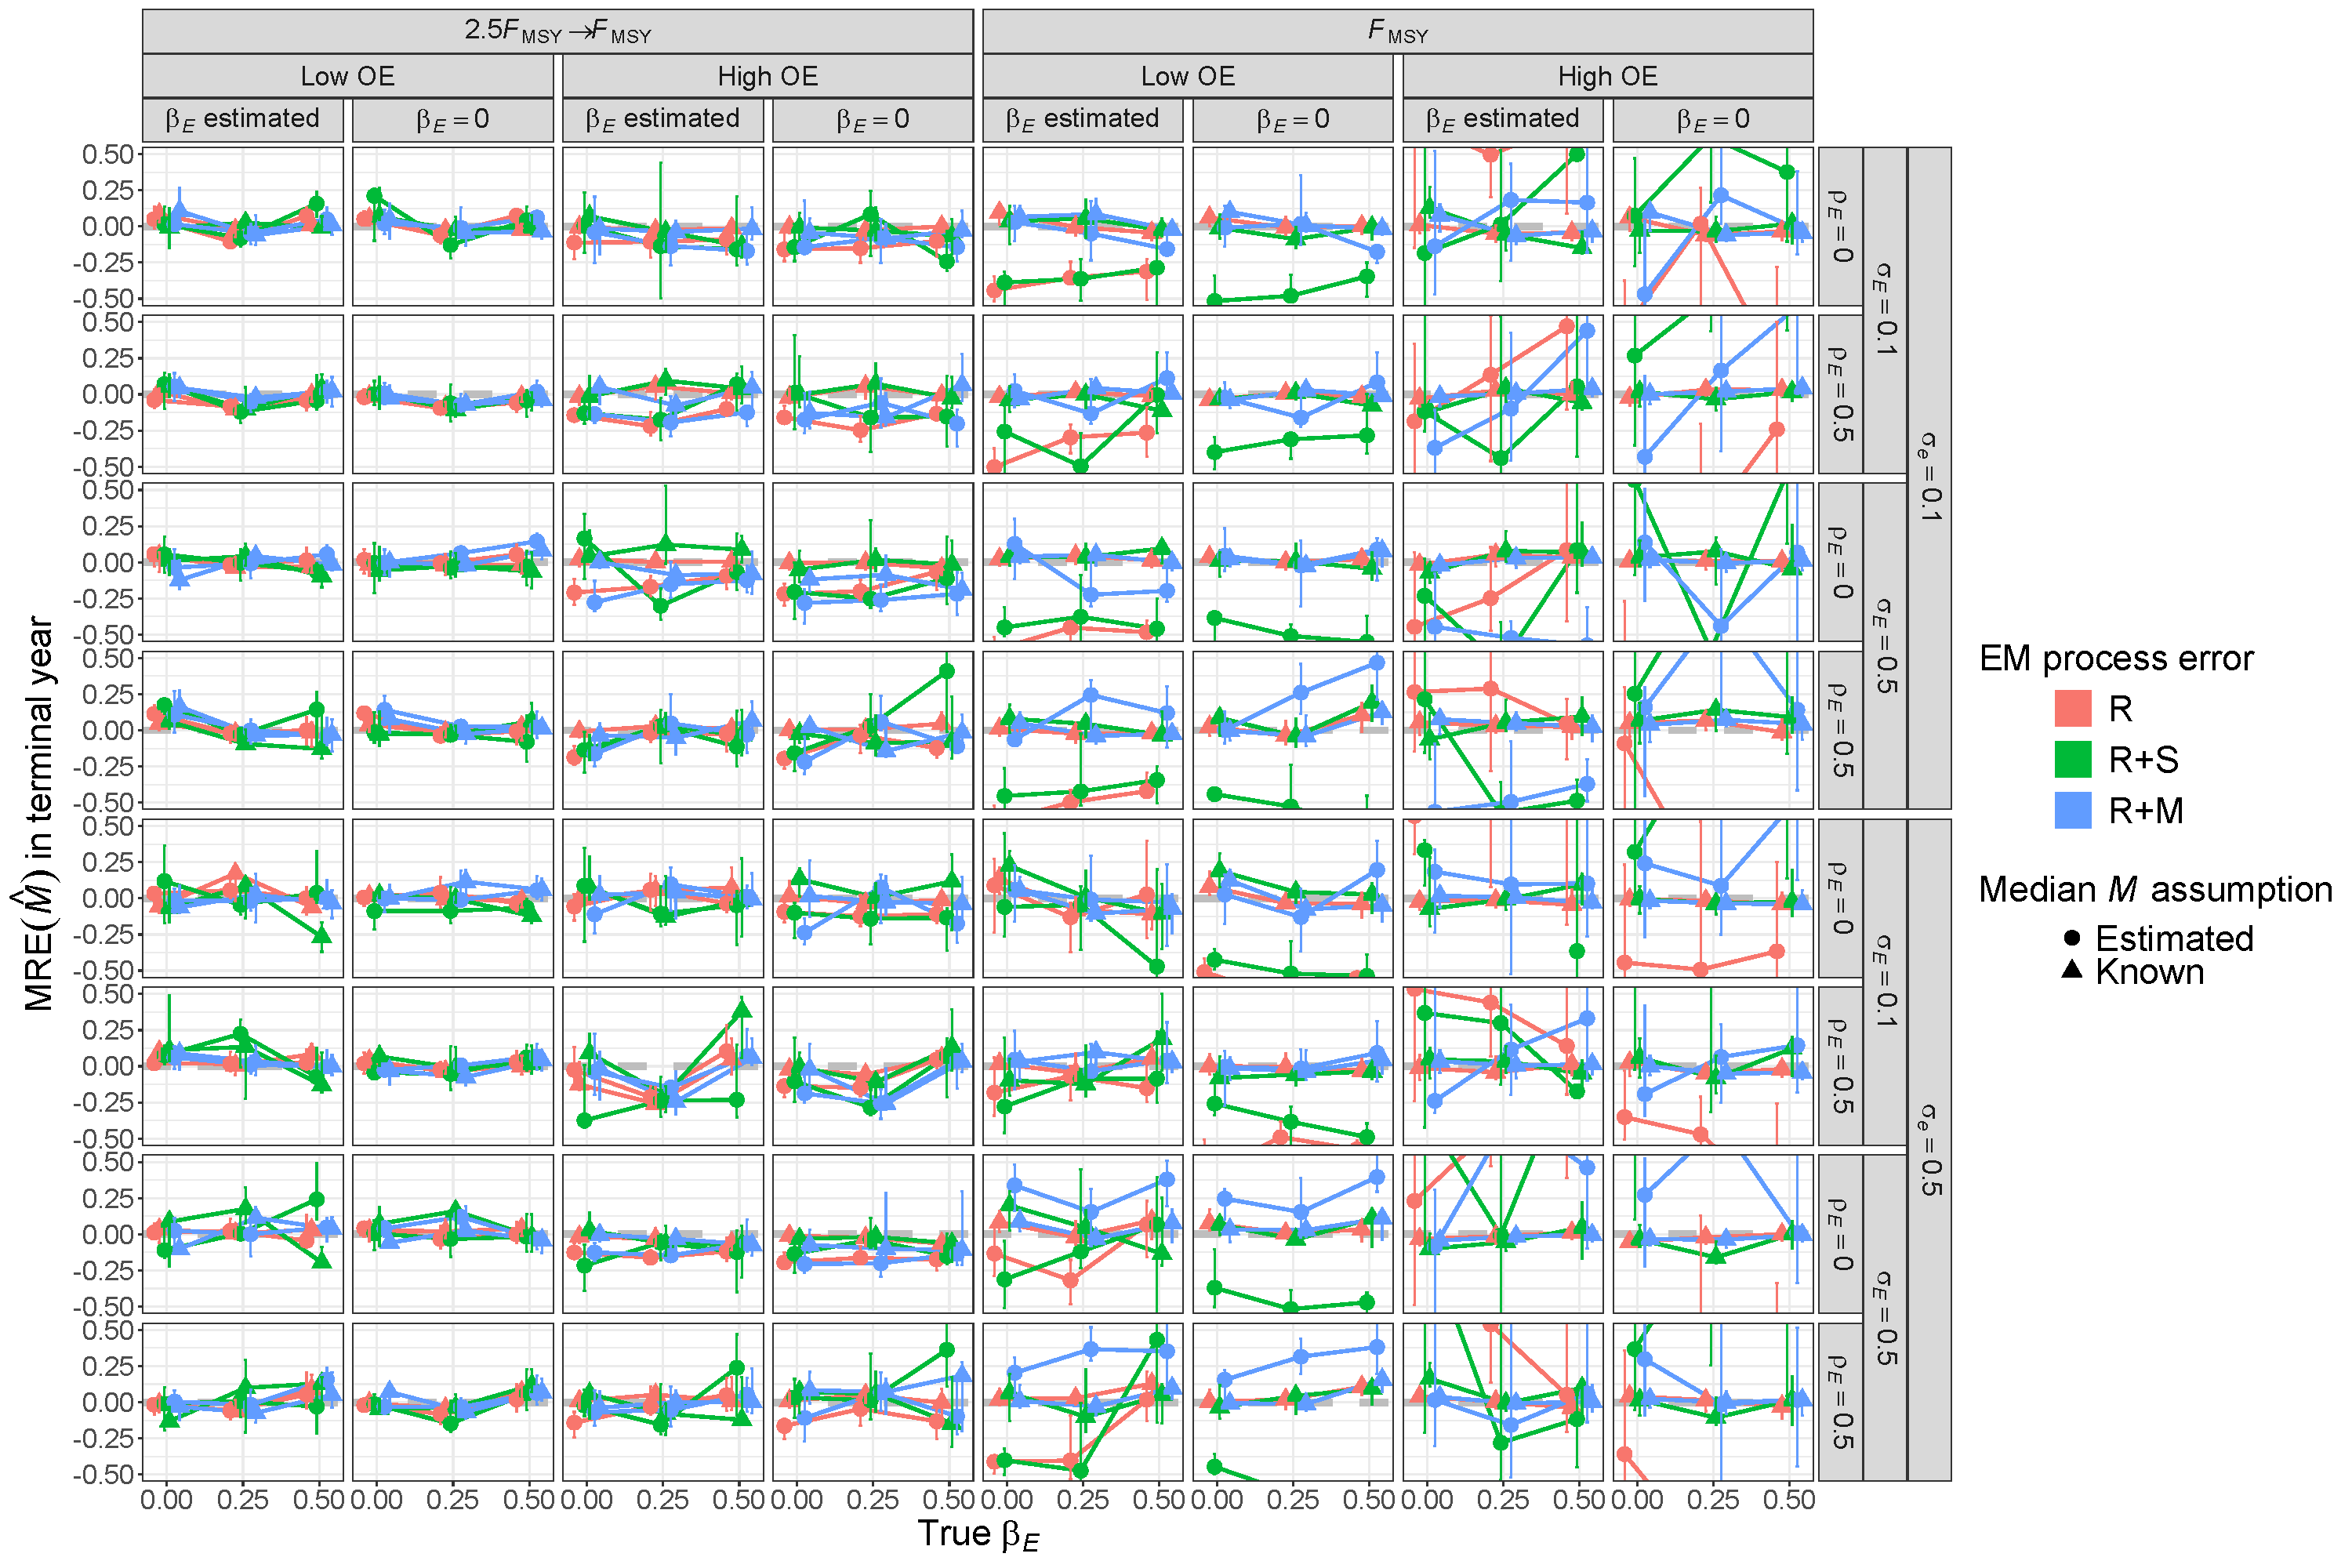
\includegraphics[height = \textheight]{terminal_year_M_bias_RMom}
\end{center}
\caption{For R+M OMs, median relative error (MRE) of estimates of natural mortality rate in the terminal year for EMs with alternative process error assumptions, treatment of covariate effect ($\beta_E = 0$ or estimated), and treatment of median natural mortality parameter ($\beta_M$ estimated or known).}\label{terminal_M_bias_RMom}
\end{figure}
\end{landscape}

\hypertarget{terminal-year-natural-mortality-rmse}{%
\subsection*{Terminal year natural mortality RMSE}\label{terminal-year-natural-mortality-rmse}}
\addcontentsline{toc}{subsection}{Terminal year natural mortality RMSE}

\begin{landscape}
\begin{figure}
\begin{center}
\includegraphics[height = \textheight]{terminal_year_M_rmse_main}
\end{center}
\caption{Root mean square error (RMSE) of estimates of natural mortality rate in the terminal year for EMs with alternative process error assumptions, treatment of covariate effect ($\beta_E = 0$ or estimated), and treatment of median natural mortality parameter ($\beta_M$ estimated or known). All OMs had low population observation error and contrast in fishing mortality.}\label{terminal_M_rmse}
\end{figure}
\end{landscape}

\begin{landscape}
\begin{figure}
\begin{center}
\includegraphics[height = \textheight]{terminal_year_M_rmse_Rom}
\end{center}
\caption{For R OMs, root mean square error (RMSE) of estimates of natural mortality rate in the terminal year for EMs with alternative process error assumptions, treatment of covariate effect ($\beta_E = 0$ or estimated), and treatment of median natural mortality parameter ($\beta_M$ estimated or known).}\label{terminal_M_rmse_Rom}
\end{figure}
\end{landscape}

\begin{landscape}
\begin{figure}
\begin{center}
\includegraphics[height = \textheight]{terminal_year_M_rmse_RSom}
\end{center}
\caption{For R+S OMs, root mean square error (RMSE) of estimates of natural mortality rate in the terminal year for EMs with alternative process error assumptions, treatment of covariate effect ($\beta_E = 0$ or estimated), and treatment of median natural mortality parameter ($\beta_M$ estimated or known).}\label{terminal_M_rmse_RSom}
\end{figure}
\end{landscape}

\begin{landscape}
\begin{figure}
\begin{center}
\includegraphics[height = \textheight]{terminal_year_M_rmse_RMom}
\end{center}
\caption{For R+M OMs, root mean square error (RMSE) of estimates of natural mortality rate in the terminal year for EMs with alternative process error assumptions, treatment of covariate effect ($\beta_E = 0$ or estimated), and treatment of median natural mortality parameter ($\beta_M$ estimated or known).}\label{terminal_M_rmse_RMom}
\end{figure}
\end{landscape}

\hypertarget{terminal-year-spawning-stock-biomass-bias}{%
\subsection*{Terminal year spawning stock biomass bias}\label{terminal-year-spawning-stock-biomass-bias}}
\addcontentsline{toc}{subsection}{Terminal year spawning stock biomass bias}

\begin{landscape}
\begin{figure}
\begin{center}
\includegraphics[height = \textheight]{terminal_year_ssb_bias_Rom}
\end{center}
\caption{For R OMs, median relative error (MRE) of estimates of spawning stock biomass (SSB) in the terminal year for EMs with alternative process error assumptions, treatment of covariate effect ($\beta_E = 0$ or estimated), and treatment of median natural mortality parameter ($\beta_M$ estimated or known).}\label{terminal_ssb_bias_Rom}
\end{figure}
\end{landscape}

\begin{landscape}
\begin{figure}
\begin{center}
\includegraphics[height = \textheight]{terminal_year_ssb_bias_RSom}
\end{center}
\caption{For R+S OMs, median relative error (MRE) of estimates of spawning stock biomass (SSB) in the terminal year for EMs with alternative process error assumptions, treatment of covariate effect ($\beta_E = 0$ or estimated), and treatment of median natural mortality parameter ($\beta_M$ estimated or known).}\label{terminal_ssb_bias_RSom}
\end{figure}
\end{landscape}

\begin{landscape}
\begin{figure}
\begin{center}
\includegraphics[height = \textheight]{terminal_year_ssb_bias_RMom}
\end{center}
\caption{For R+M OMs, median relative error (MRE) of estimates of spawning stock biomass (SSB) in the terminal year for EMs with alternative process error assumptions, treatment of covariate effect ($\beta_E = 0$ or estimated), and treatment of median natural mortality parameter ($\beta_M$ estimated or known).}\label{terminal_ssb_bias_RMom}
\end{figure}
\end{landscape}

\hypertarget{terminal-year-spawning-stock-biomass-rmse}{%
\subsection*{Terminal year spawning stock biomass RMSE}\label{terminal-year-spawning-stock-biomass-rmse}}
\addcontentsline{toc}{subsection}{Terminal year spawning stock biomass RMSE}

\begin{landscape}
\begin{figure}
\begin{center}
\includegraphics[height = \textheight]{terminal_year_ssb_rmse_main}
\end{center}
\caption{Root mean square error (RMSE) of estimates of spawning stock biomass in the terminal year for EMs with alternative process error assumptions, treatment of covariate effect ($\beta_E = 0$ or estimated), and treatment of median natural mortality parameter ($\beta_M$ estimated or known). All OMs had low population observation error and contrast in fishing mortality.}\label{terminal_ssb_rmse}
\end{figure}
\end{landscape}

\begin{landscape}
\begin{figure}
\begin{center}
\includegraphics[height = \textheight]{terminal_year_ssb_rmse_Rom}
\end{center}
\caption{For R OMs, root mean square error (RMSE) of estimates of spawning stock biomass in the terminal year for EMs with alternative process error assumptions, treatment of covariate effect ($\beta_E = 0$ or estimated), and treatment of median natural mortality parameter ($\beta_M$ estimated or known).}\label{terminal_ssb_rmse_Rom}
\end{figure}
\end{landscape}

\begin{landscape}
\begin{figure}
\begin{center}
\includegraphics[height = \textheight]{terminal_year_ssb_rmse_RSom}
\end{center}
\caption{For R+S OMs, root mean square error (RMSE) of estimates of spawning stock biomass in the terminal year for EMs with alternative process error assumptions, treatment of covariate effect ($\beta_E = 0$ or estimated), and treatment of median natural mortality parameter ($\beta_M$ estimated or known).}\label{terminal_ssb_rmse_RSom}
\end{figure}
\end{landscape}

\begin{landscape}
\begin{figure}
\begin{center}
\includegraphics[height = \textheight]{terminal_year_ssb_rmse_RMom}
\end{center}
\caption{For R+M OMs, root mean square error (RMSE) of estimates of spawning stock biomass in the terminal year for EMs with alternative process error assumptions, treatment of covariate effect ($\beta_E = 0$ or estimated), and treatment of median natural mortality parameter ($\beta_M$ estimated or known).}\label{terminal_ssb_rmse_RMom}
\end{figure}
\end{landscape}

\hypertarget{terminal-year-fishing-mortality-bias}{%
\subsection*{Terminal year fishing mortality bias}\label{terminal-year-fishing-mortality-bias}}
\addcontentsline{toc}{subsection}{Terminal year fishing mortality bias}

\begin{landscape}
\begin{figure}
\begin{center}
\includegraphics[height = \textheight]{terminal_year_F_bias_main}
\end{center}
\caption{Median relative error (MRE) of estimates of fully-selected fishing mortality ($F$) in the terminal year for EMs with alternative process error assumptions, treatment of covariate effect ($\beta_E = 0$ or estimated), and treatment of median natural mortality parameter ($\beta_M$ estimated or known). All OMs had low population observation error and contrast in fishing mortality.}\label{terminal_F_bias}
\end{figure}
\end{landscape}

\begin{landscape}
\begin{figure}
\begin{center}
\includegraphics[height = \textheight]{terminal_year_F_bias_Rom}
\end{center}
\caption{For R OMs, median relative error (MRE) of estimates of fully-selected fishing mortality ($F$) in the terminal year for EMs with alternative process error assumptions, treatment of covariate effect ($\beta_E = 0$ or estimated), and treatment of median natural mortality parameter ($\beta_M$ estimated or known). All OMs had low observation error and contrast in fishing mortality.}\label{terminal_F_bias_Rom}
\end{figure}
\end{landscape}

\begin{landscape}
\begin{figure}
\begin{center}
\includegraphics[height = \textheight]{terminal_year_F_bias_RSom}
\end{center}
\caption{For R+S OMs, median relative error (MRE) of estimates of fully-selected fishing mortality ($F$) in the terminal year for EMs with alternative process error assumptions, treatment of covariate effect ($\beta_E = 0$ or estimated), and treatment of median natural mortality parameter ($\beta_M$ estimated or known). All OMs had low observation error and contrast in fishing mortality.}\label{terminal_F_bias_RSom}
\end{figure}
\end{landscape}

\begin{landscape}
\begin{figure}
\begin{center}
\includegraphics[height = \textheight]{terminal_year_F_bias_RMom}
\end{center}
\caption{For R+M OMs, median relative error (MRE) of estimates of fully-selected fishing mortality ($F$) in the terminal year for EMs with alternative process error assumptions, treatment of covariate effect ($\beta_E = 0$ or estimated), and treatment of median natural mortality parameter ($\beta_M$ estimated or known). All OMs had low observation error and contrast in fishing mortality.}\label{terminal_F_bias_RMom}
\end{figure}
\end{landscape}

\hypertarget{terminal-year-fishing-mortality-rmse}{%
\subsection*{Terminal year fishing mortality RMSE}\label{terminal-year-fishing-mortality-rmse}}
\addcontentsline{toc}{subsection}{Terminal year fishing mortality RMSE}

\begin{landscape}
\begin{figure}
\begin{center}
\includegraphics[height = \textheight]{terminal_year_F_rmse_main}
\end{center}
\caption{Root mean square error (RMSE) of estimates of fully-selected fishing mortality ($F$)  in the terminal year for EMs with alternative process error assumptions, treatment of covariate effect ($\beta_E = 0$ or estimated), and treatment of median natural mortality parameter ($\beta_M$ estimated or known). All OMs had low population observation error and contrast in fishing mortality.}\label{terminal_F_rmse}
\end{figure}
\end{landscape}

\begin{landscape}
\begin{figure}
\begin{center}
\includegraphics[height = \textheight]{terminal_year_F_rmse_Rom}
\end{center}
\caption{For R OMs, root mean square error (RMSE) of estimates of fully-selected fishing mortality ($F$)  in the terminal year for EMs with alternative process error assumptions, treatment of covariate effect ($\beta_E = 0$ or estimated), and treatment of median natural mortality parameter ($\beta_M$ estimated or known).}\label{terminal_F_rmse_Rom}
\end{figure}
\end{landscape}

\begin{landscape}
\begin{figure}
\begin{center}
\includegraphics[height = \textheight]{terminal_year_F_rmse_RSom}
\end{center}
\caption{For R+S OMs, root mean square error (RMSE) of estimates of fully-selected fishing mortality ($F$)  in the terminal year for EMs with alternative process error assumptions, treatment of covariate effect ($\beta_E = 0$ or estimated), and treatment of median natural mortality parameter ($\beta_M$ estimated or known).}\label{terminal_F_rmse_RSom}
\end{figure}
\end{landscape}

\begin{landscape}
\begin{figure}
\begin{center}
\includegraphics[height = \textheight]{terminal_year_F_rmse_RMom}
\end{center}
\caption{For R+M OMs, root mean square error (RMSE) of estimates of fully-selected fishing mortality ($F$)  in the terminal year for EMs with alternative process error assumptions, treatment of covariate effect ($\beta_E = 0$ or estimated), and treatment of median natural mortality parameter ($\beta_M$ estimated or known).}\label{terminal_F_rmse_RMom}
\end{figure}
\end{landscape}

\end{document}
